%==================================================================================================
%   Nuno de Sousa Template 1.0
%   -------------------------
%   This template is based on Luke template.
%
%   -------------------------
%   Last Updated: 2014-01-28
%   Contact: nuno.teixeira@uam.es
%==================================================================================================
%
%==================================================================================================
% DOCUMENT SETUP
%==================================================================================================
\documentclass[10pt,twoside]{book}
%
%
%Set to 'print' for printed version, use 'net' for online version
\def\thesisversion{print}
%
%==================================================================================================
% PACKAGES
%==================================================================================================
\usepackage{NunoThesis}                             %Import Thesis base style
%input{PhDMacros}                                   %Thesis specific macros
%
%==================================================================================================
% THESIS PROPERTIES (Modifiy these fields with your details)
%==================================================================================================
\def\thesisauthor{Nuno de Sousa}                     %Author
\def\thesistitle{Light scattering in disordered and nonreciprocal media}               %Title
\def\thesishandin{September 2014}                        %Submission date (Day-Month}
\def\thesisdegree{PhD}                              %Degree ('B.Eng', 'B.Sc.', 'M.Sc.' or 'PhD')
\def\thesisyear{2014}                               %Submission year
\def\thesisnumber{}                             %Serial number (do not include year)
\def\thesisISSN{}                                   %ISSN number
\def\thesiskeywords{Keywords are, comma separated}  %PDF keywords
\derivethesisprops                                  %Derive dependent properties
%
%==================================================================================================
% SECTION NUMBERING SETUP
%==================================================================================================
\setcounter{tocdepth}{2}                            %2 adds sections up to subsections
\setcounter{secnumdepth}{3}                         %Subsubsections get a number when this is 3
%
%==================================================================================================
% THESIS STRUCTURE  (Modify to include more chapters etc)
%==================================================================================================
\begin{document}
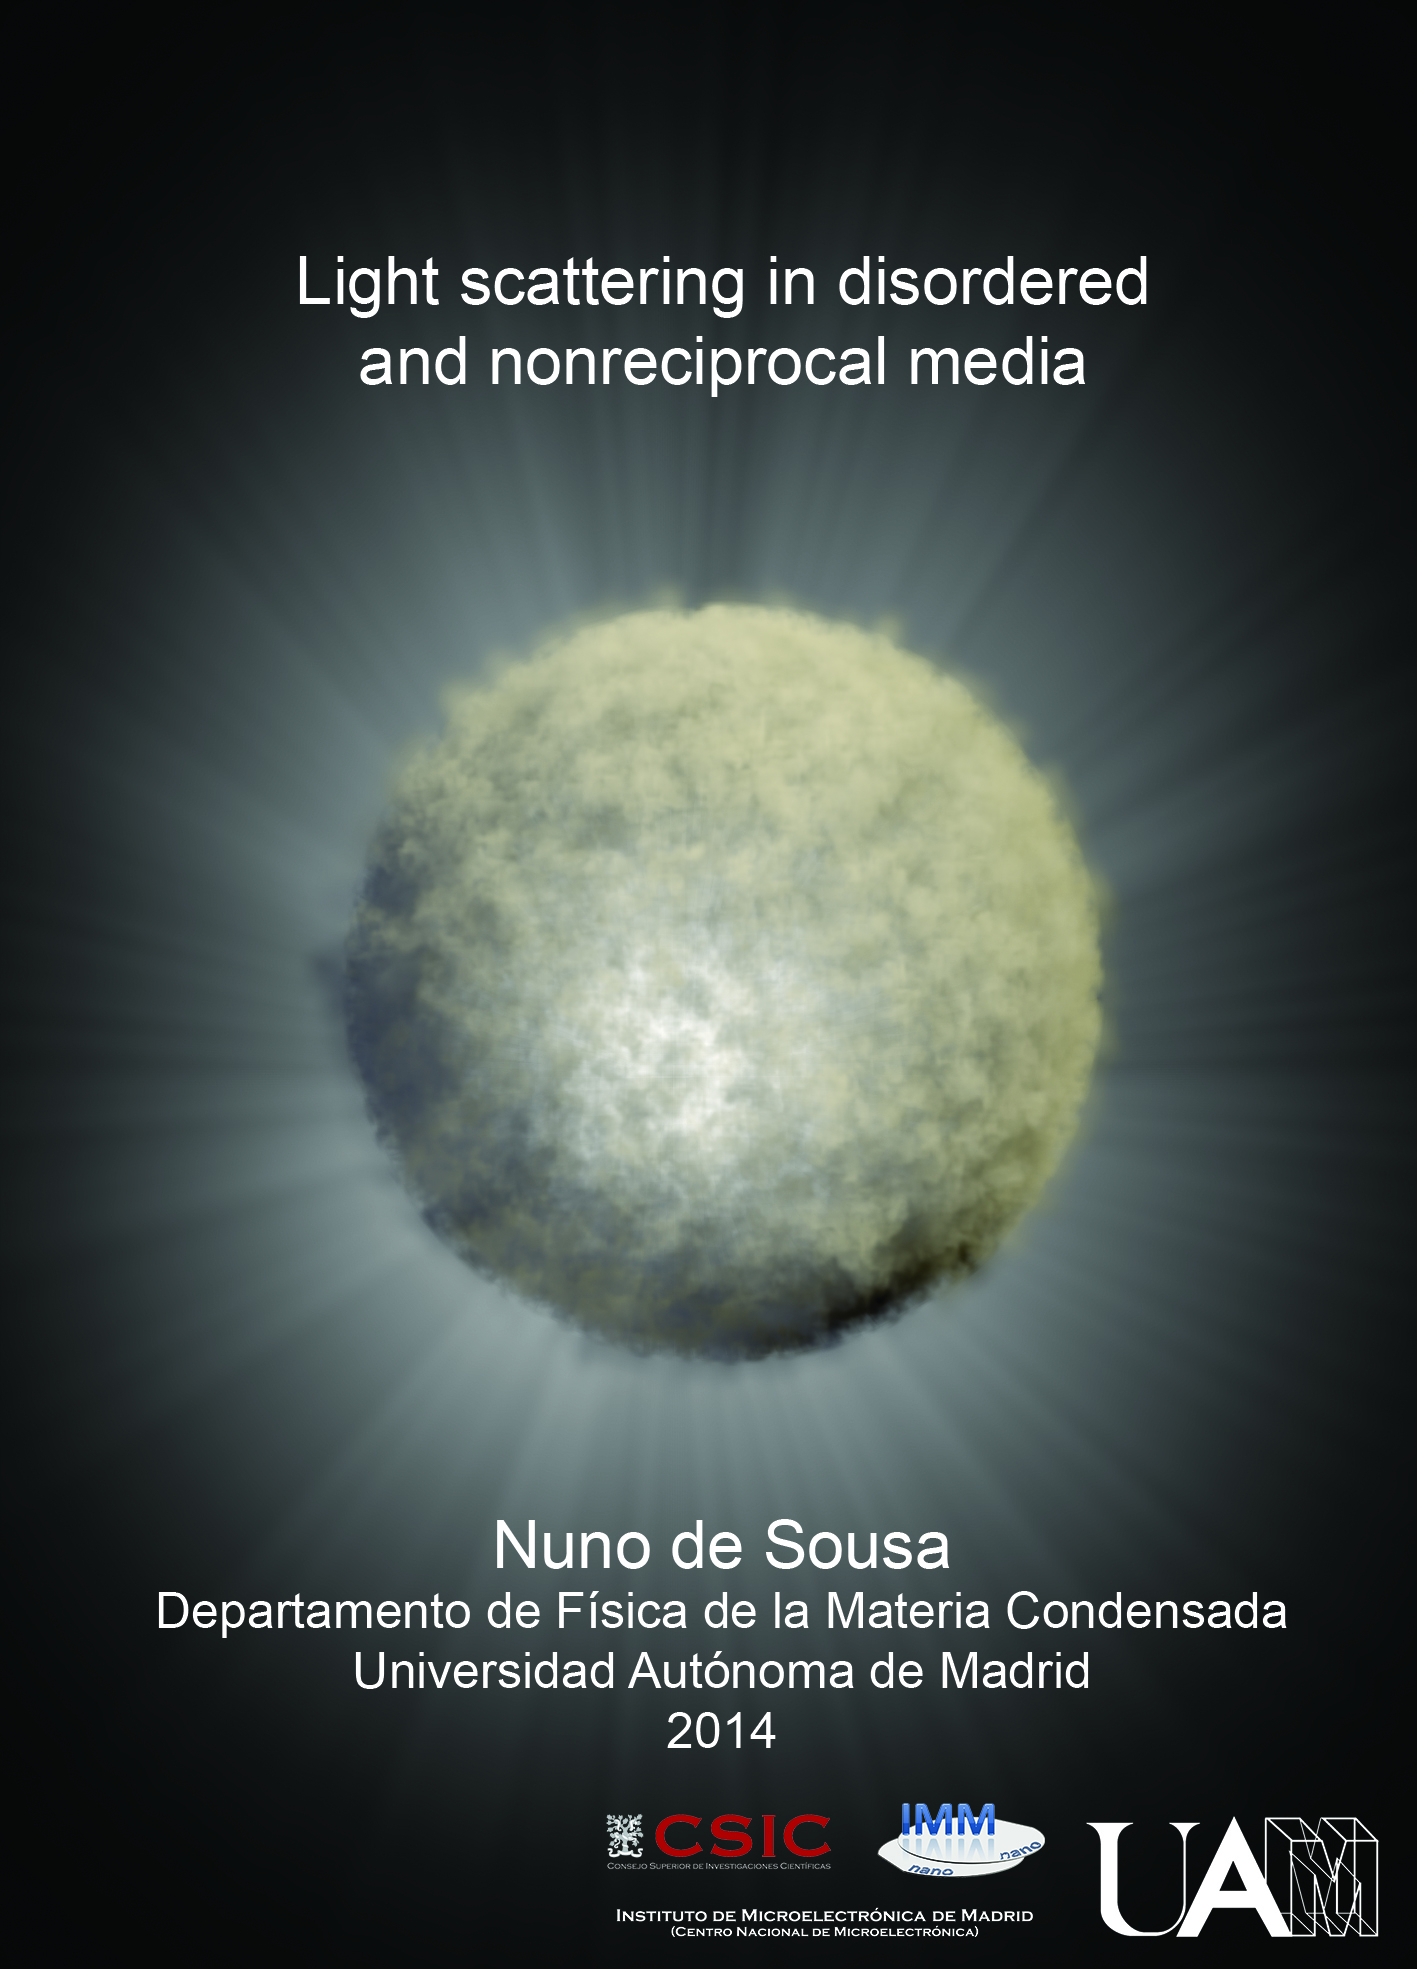
\includepdf{figures/cover.pdf}
\newpage\null\thispagestyle{empty}
\newpage\null\thispagestyle{empty}
%------------------------
%Pre-frontmatter material
%------------------------
\prefrontmatter
%--------------------
%Frontmatter material
%--------------------
\frontmatter
\pagenumbering{roman}                               %Set frontmatter numbering style
\newpage\null\thispagestyle{empty}
\newpage\null\thispagestyle{empty}
\chapter{Foreword}


The work of this thesis is focused on the study of light scattering in random correlated systems, on one side, and in magneto-optical media, on the other.\\
Since the foundations of the electromagnetic theory, efforts have been made to understand how light interacts with complex environments. Until now, most works are centred in either perfectly ordered or disordered systems. In these extreme cases a rich phenomenology was found, such as the existence of photonic bandgaps in photonic crystals or weak and strong localisation in disordered systems. Between these two limits, perfectly ordered and disordered systems, are the random correlated systems. Although it is known that correlations in disordered media can play an important role in the wave transport properties, these random correlated systems remain largely unexplored. Examples such as the conductivity of liquid metals in solid state physics, or light transport properties in photonic systems governed by short-range structural correlations, like in cornea, demonstrate the importance of these media.\\
Being dominated by multiple light scattering, light transport and emission are closely related phenomena. However, much more attention has been given to the first over the second. In recent years a small number of works have shown the importance of light emission by point sources for the study of correlations in random systems. In particular, these take advantage of the proportionality of the single emitter decay rate fluctuations with the local density of states fluctuations. Because short-range correlations can alter the single emitter decay rate statistics, light scattering in the near field is crucial for the understanding of correlated random systems.\\
The lack of completeness in the study of emission dynamics extends from simple geometry systems to complex structures. An interesting example is the inclusion of reciprocity symmetry breaking in well known structures, like in emitter-antenna systems. A way of introducing nonreciprocity effects is by applying an external magnetic field and considering the magnetisation properties of the materials that form the system. The effect that involves the modification of the optical properties by the application of a magnetic field is known as magneto-optical effect. 
This is of special importance in hybrid metallic systems that support at the same time plasmon excitations (magnetoplasmonic systems), giving rise to plasmon enhanced magneto-optical activity. 
These structures are particularly interesting because can be applied in biology, sensing and telecommunications. Due to the available fabrication and characterisation technology, it is possible to design and implement complex structures that take into account this magneto-optical effect. Nevertheless, the optimisation processes are directly related to the modelling ability of such systems.\\
The aim of this thesis is to clarify some open questions in magnetoplasmonic systems and random correlated systems. The thesis is organised in two parts.\\
In the first part, we want to understand, through simple physical models, the rich phenomenology obtained in hybrid magnetoplasmonic systems. In particular, we are interested in determine the exact role of interactions between forming elements of the systems and their contribution to the global magneto-optical response.\\
We will also address the antenna effect in the presence of magneto-optical activity. The considered model is an emitter-antenna system in which the antenna supports a plasmon resonance and shows magneto-optical activity.\\
In the second part of this thesis we study the emission lifetime in thin layers of strongly scattering media with non-trivial correlations: search for evidences of peculiar statistical distributions in lifetime statistics (long tail distributions, multimodal, etc). The objective is trying to prove that not only the parameters governing the statistical distributions of lifetimes are non-universal, but also the nature of the distributions themselves depend on the details of the system. \\
Finally, we focus our attention on the light emission dynamics (lifetimes or emission rate statistics) in three-dimensional systems with strong structural correlations undergoing structural phase transitions. The objective is trying to link the statistical properties of emission dynamics with the thermodynamics of the system and prove that there are fundamental differences between lifetime statistics and transport properties.\\





                                   %English summary of Thesis
\markboth{}{}                                       %Set headings (left)(right)
\chapter{Pr�logo}

El trabajo de esta tesis se centra en el estudio del scattering de luz en sistemas aleatorios correlacionados, por un lado, y en medios magneto-�pticos, por el otro. 
Desde los inicios de la teor�a electromagn�tica, se han hecho esfuerzos para entender c�mo interact�a la luz con entornos complejos. Hasta ahora, la mayor�a de los estudios se basan en sistemas perfectamente ordenados o completamente desordenados. En estos casos se encontraron fen�menos muy relevantes del punto de vista cientifico, tales como la existencia de bandgaps en cristales fot�nicos o la localizaci�n d�bil y fuerte en sistemas desordenados. Entre estos dos l�mites, sistemas perfectamente ordenados y desordenados, se encuentran los sistemas aleatorios correlacionados. Aunque se sabe que las correlaciones en medios desordenados pueden jugar un papel importante en las propiedades de transporte de ondas, estos sistemas aleatorios correlacionados no han sido estudiados en detalle. Ejemplos tales como la conductividad en metales l�quidos, o las propiedades de transporte de luz en sistemas fot�nicos regidas por correlaciones estructurales de corto alcance, demuestran la importancia de estos medios. \\
Al ser governados por el scattering m�ltiple de la luz, el transporte y emisi�n de luz son fen�menos estrechamente relacionados. Sin embargo, se ha prestado m�s atenci�n al primero sobre el segundo. En los �ltimos a�os un peque�o n�mero de trabajos han demostrado la relevancia de la emisi�n de luz por fuentes puntuales para el estudio de las correlaciones en sistemas aleatorios. En particular, estos se aprovechan de la proporcionalidad de la tasa de decaimiento radiativo de un solo emisor con las fluctuaciones de la densidad local de estados para estudiar el efecto de las correlaciones. Debido a que las correlaciones de corto alcance pueden alterar la tasa de decaimiento radiativo de un solo emisor, el scattering de la luz en el campo cercano es un elemento crucial para la comprensi�n de los sistemas aleatorios correlacionados.\\
La falta de exhaustividad en el estudio de la din�mica de emisi�n se extiende desde sistemas geom�tricos simples hasta estructuras complejas. Un ejemplo interesante es la ruptura de reciprocidad en estructuras conocidas, como en los sistemas emissor-antenna. Una forma de introducir efectos no rec�procos es mediante la aplicaci�n de un campo magn�tico externo y teniendo en cuenta las propiedades de magnetizaci�n de los materiales que conforman el sistema. El efecto que involucra la modificaci�n de las propiedades �pticas mediante la aplicaci�n de un campo magn�tico se conoce como efecto magneto-�ptico. Esto es de especial importancia en sistemas met�licos h�bridos que presentan al mismo tiempo excitaciones de plasmones (sistemas magnetoplasm�nicos), dando lugar a una mayor actividad magneto-�ptica debido a la excitaci�n del plasm�n. Estas estructuras son particularmente interesantes porque pueden tener aplicaciones en biolog�a, sistemas de detecci�n y telecomunicaciones. Debido a los avances en fabricaci�n y tecnolog�as de caracterizaci�n, es posible dise�ar e implementar estructuras complejas que hacen uso del efecto magneto-�ptico. Sin embargo, los procesos de optimizaci�n est�n directamente relacionados con la capacidad de simular estos sistemas.\\ 
Esta tesis tiene como objetivo esclarecer algunas cuestiones abiertas acerca de sistemas magnetoplasm�nicos y sistemas aleatorios correlacionados. La tesis se estructura en dos partes. En la primera, se pretende explicar a trav�s de modelos f�sicos simples, los fen�menos que ocurren en sistemas magnetoplasm�nicos h�bridos. En particular, estamos interesados en determinar el papel de las interacciones entre los elementos que forman los sistemas y su contribuci�n a la respuesta magneto-�ptica global. 
Ademas, estudiaremos el efecto de la antena en presencia de actividad magneto-�ptica. El modelo considerado es un sistema emissor-antena en el que la antena presenta una resonancia de plasm�n y muestra la actividad magneto-�ptica. \\
En la segunda parte de esta tesis se estudia el tiempo de vida de un emisor en capas delgadas formadas por part�culas fuertemente dispersoras con correlaciones no triviales: la b�squeda de evidencias de distribuciones peculiares en la estad�stica de tiempo de vida (distribuciones de cola larga, \textit{i.e.}, que tiene muchos eventos raros, multimodales, etc). El objetivo es tratar de demostrar que no s�lo los par�metros que rigen las distribuciones estad�sticas de tiempo de vida son no universales, sino tambi�n que la naturaleza de las distribuciones en s� mismas dependen de detalles del sistema. 
Por �ltimo, nos centramos en la din�mica de emisi�n de luz (tiempo de vida o estad�stica de tasa de emisi�n de radiaci�n) en sistemas tridimensionales con fuertes correlaciones estructurales sometidos a transiciones de fase. El objetivo es tratar de vincular las propiedades estad�sticas de la emisi�n din�mica con las propiedades termodin�micas del sistema y demostrar que existen diferencias fundamentales entre la estad�stica de tiempo de vida y las propiedades de transporte.
                                   %Spanish summary of Thesis
%\markboth{}{}                                       %Set headings (left)(right)
%\chapter{Preface}

This thesis was prepared at the department of Informatics and Mathematical Modelling at the Technical University of Denmark in fulfilment of the
requirements for acquiring an M.Sc. in Informatics.

The thesis deals with ...

The thesis consists of ...
%==================================================================================================
% SIGNATURE AREA
%==================================================================================================
                                     %Preface
\markboth{}{}                                       %Set headings (left)(right)
\chapter{Acknowledgements}

%\vspace*{0}
Ao longo destes anos muitas pessoas e institui��es contribu�ram directa ou indirectamente para esta tese.\\
Come�o por quem foi crucial para este trabalho, os meus directores de tese, Antonio Garc�a e Luis Froufe, e meu tutor da Universidade Aut�noma de Madrid, Juan Jos� Saenz. Antes de tudo, agrade�o-vos por me terem aceite como vosso aluno, terem acreditado em mim e por fazerem com que esta tese seja uma realidade. Agrade�o-vos por toda a paci�ncia (e que n�o foi pouca), dedica��o e persist�ncia. Por partilharem o encanto menos evidente da f�sica, por me terem mostrado e ensinado tanto, mais do que algum dia pude imaginar. Devo real�ar a vossa capacidade de trabalho, dom�nio das ferramentas e a vossa intui��o, que s�o realmente impressionantes. Sabeis fazer arte como poucos. Deste per�odo n�o me posso esquecer da amizade constru�da, das reuni�es de "Viernes", dos meses que passamos ao quadro discutindo ou das bonitas e floreadas express�es castelhanas que me ensinaram!
Poderia perder-me em um sem-fim de palavras, mas nunca conseguiria expressar a dimens�o do meu agradecimento. Assim, muito obrigado.\\
Quero agradecer ao departamento de F�sica da Mat�ria Condensada, e em particular � Elsa e � Luisa, pela forma como me acolheram e acompanharam, por facilitarem as melhores condi��es para trabalhar.\\
Ao grupo do Cefe Lopez do Instituto de Ci�ncia dos Materiais de Madrid e ao grupo de Jos� Antonio S�nchez-Gil do Instituto de Estrutura da Mat�ria, pelo per�odo enriquecedor que me proporcionaram (estive quase um ano em cada instituto) e por fazerem com que a minha est�ncia fosse t�o agrad�vel. \\
%\vfill % equivalent to \vspace{\fill}
%\clearpage
%\vspace*{0.5cm}
Ao Instituto de Microelectr�nica de Madrid, em particular aos elementos do Grupo de Magnetoplasm�nica, a Gaspar Armelles, a Alfonso Cebollada, a Maria Uju�, a Jos� Miguel Garc�a Mart�n e a David Menezes pela oportunidade de poder trabalhar e colaborar convosco.\\
Tamb�m quero agradecer a David Schmool, a Hamid Kachkachi e a Fran�ois Vernay por me terem recebido em Perpignan, especialmente pelas discuss�es interessantes que proporcionaram.\\
Quero agradecer � Scixel pela fant�stica capa que realizou para esta tese. Tamb�m foram v�rias as vezes que recorri � sua ajuda para criar imagens usadas nos v�rios trabalhos, tendo sempre encontrado total disponibilidade e um servi�o incompar�vel. "You do the Science, we arrange the pixels". \\
Bom, vamos � parte mais pessoal. Agrade�o �s pessoas que mais pr�ximo estiveram durante este per�odo. Porque foram tantos s�tios por onde passei e tantas pessoas que conheci, espero que entendam alguma omiss�o. \\
Come�o pelo meu grupo: aos seniores, a Pedro e a Manuel, por estarem permanentemente dispon�veis para ajudar e por tornarem os almo�os muito mais interessantes. \\
Ao Kike, agora CEO/CAO/etc. da Scixel, por ser um dos gajos mais porreira�os que conheci aqui em Espanha, ser um �ptimo companheiro de gabinete, e ter uma habilidade brutal para ajudar os amigos a fazer imagens. Agrade�o tamb�m a tua dedica��o na hora de partilhares o melhor que o castelhano tem para oferecer. � Silvia, minha irm� cientifica. Sempre bem disposta e com vontade de discutir sobre f�sica. Por ser minha conselheira em todos os assuntos, aguentar as minhas lamenta��es quando estava doente, e ser bastante fixolas! Aos dois, estou grato pela vossa amizade.\\
Aos meus companheiros de gabinete Irene, Laura, Jorge, Carlos e Maria e aos Roldanes, Carlos e Cristina. A todos v�s, agrade�o-vos a disponibilidade e companheirismo. Em todas as recorda��es do gabinete voc�s est�o presentes. Ao Miztli, por ter sido um �ptimo companheiro e extremamente paciente para as minhas d�vidas tensoriais. N�o te esque�as de voltar a Espanha para se dar o combate do s�culo: Ca�oncito Pum Pum Sousa vs Hurracan Dr. Yepez.\\
Ao Jonathan, meu companheiro de armas asturiano, que esteve comigo parte deste percurso, da electr�nica � escrita da tese. Sinto-me afortunado por te ter conhecido.\\
%\vfill % equivalent to \vspace{\fill}
%\clearpage
%\newpage
%\vspace*{0cm}
Aos que conheci por c� e que de alguma forma contribu�ram para este tese. \\
Ao Fermento, que depois de partilhamos casa durante dois anos, passamos de desconhecidos a bons amigos. Por algum motivo, as melhores recorda��es que tenho contigo s�o com uma Guinness na m�o! \\
Ao Jorge, meu tradutor oficial e que me deu a conhecer os tamarindos, por todos os finais de dia que fomos relaxar, bebendo "s� uma cervejinha".\\
� Mariana, ao Chon, Elias, Maki, Filipe e demais piratas que fui conhecendo aos longo dos anos e que preencheram a minha vida de hist�rias e bons momentos.\\
N�o posso deixar de agradecer aos Ranilla-Ziniewicz, Queir�s (irmandade e Co.) e Apolin�rio. �s minhas fam�lias Portuguesas, Santos, Sousa, Carvalho de Matos, Matos Silvestre e Fonseca Matos. A todos v�s, obrigado pelo apoio.\\
Aos que c� n�o est�o, ao Am�rico e ao Torcato. Provavelmente as pessoas que mais me influenciaram e estimularam a minha curiosidade. Sou fruto do seu trabalho e em grande medida esta tese deve-se a eles.\\
Por fim, a fam�lia, o meu irm�o Jo�o e a minha m�e No�mia. Por me apoiarem incondicionalmente, por estarem sempre ao meu lado, suportarem o meu mau humor e as crises de stress. Por me incentivarem sempre a continuar e nunca parar. Pelo amor e carinho de sempre. (Jo�o, a partir de hoje todas as camisas brancas s�o tuas!)\\
A C�tia, sem d�vida a pessoa que de mais perto viveu e sofreu com esta tese. Pela tua paci�ncia, carinho e dedica��o. Pela loucura de deixares tudo e vires para Madrid. Por teres estado ao meu lado em alguns dos piores e melhores momentos. Por quereres que eu esteja ao teu lado.

\vspace{10mm}
\begin{center}
    \hspace{20mm} Madrid, \thesishandin %-\thesisyear
    \vspace{2mm}
    \newline
  %Update signature image file in line below
    
\includegraphics[scale=0.1]{figures/Signature}
\end{center}
%\begin{flushright}
%    \centerline{\thesisauthor}
%\end{flushright}
% % % EOF % % %

%\vfill % equivalent to \vspace{\fill}
%\clearpage           %Acknowledgements
\markboth{}{}                                       %Set headings (left)(right)
%------------------
% Table of contents
%------------------
\newpage\mbox{}\newpage
\chaptermark{Contents}
\pdfbookmark{\contentsname}{toc}
\renewcommand{\sectionmark}[1]{\markright{#1}}
\sectionmark{Contents}
\addtolength{\parskip}{-\baselineskip}
\tableofcontents
\addtolength{\parskip}{\baselineskip}
\renewcommand{\sectionmark}[1]{\markright{\thesection\ #1}}
%-------------
% Main content
%-------------
\mainmatter
\chapter{Introduction \label{chap1}}

Scattering, absorption and emission of light are central problems in science and engineering. Examples of these phenomena can be found, for instance, in earth's atmosphere, such as the colour of the sky or the clouds, in colloidal suspensions such as milk, or in biological tissues such as eyes. Because light scattering is strongly dependent of the particles size, shape and refractive index, scattering measurements are a crucial tool for astrophysics, biology, and engineering.\\
In the last decades, with the advent of nanophotonics, this topic has gain popularity. Nanophotonics or nano-optics is the branch of optics devoted to the study of light interaction with matter at the nanometer scale. The typical wavelength of the electromagnetic radiation lies between the ultraviolet ($300nm$)  and the near-infrared ($1.4\mu m$). This range of the electromagnetic spectrum is of special interest because the photon's energy lies in the range of the electronic transitions of matter. The human vision is adapted to detect radiation at these wavelengths, thus resulting in the diversity of colours. At these dimensions the electromagnetic radiation is well described by the wave picture and the use of classical theory of fields based on Maxwell's equations is suitable. 
%However, the small dimensions of matter require a quantum description of its properties. So, in nanophonics, is usual the use of a semiclassical theory, where classical theory of fields is combined with the quantum picture of matter.\\

%The aim of this thesis is the study of light interaction with nonreciprocal media and disordered systems, both at nanometric scale. In the first part we study emission and transport phenomena in magnetoplasmonic nanostructures, where the influence of an external magnetic field in the global behaviour of the system is analysed. The second part is devoted to the study of emission phenomenon in random correlated systems. 

\section{Light scattering with matter}

The propagation of light in a homogeneous and linear medium is done in straight paths. When inhomogeneities are present in the system, like particles or interfaces, light can be deflected from its straight path and consequently the direction of propagation changes.\\ 
Analysing the scattering systems, two different regimes can be identified: single and multiple scattering. In the single scattering regime, the field resulting from the interaction is described by the sum of the scattered fields (directly scattered, only once) from each of the scatterers in the system. Multiple scattering enters when the previous picture breaks down. In this case, the contributions of "partial waves" that have interacted with several scatterers are relevant. In the multiple scattering there is interplay between density, scattering cross section and dimensionality of the problem.\\
%When scattering occurs due to the presence of only one scatterer, or if in the system are present many scatterers but the scattered light don't interfere again with other scatterers, the system is in the single scattering regime; when light interacts many times with scatterers is called multiple scattering.\\
The treatment of light interaction requires different descriptions, depending of object scale under study. For objects with dimensions much bigger than the wavelength, the interaction can be described by geometrical optics, which considers light propagation in terms of rays.
This simplification is an excellent approximation to address many problems at the macroscale, like reflection or refraction phenomena including optical systems. It is used to describe the geometrical aspects
of imaging, including optical aberrations. However, it fails when  diffraction or interference phenomena are relevant in the system.\\
For objects with dimensions similar to the wavelength, it is common to consider the formal solution of Maxwell's equations with appropriate boundary conditions \cite{hulst1957light, bohren2008absorption}.
This approach is very useful due to the existence of exact solutions, although can only be applied to a small number of simple shapes such as spheres (usually called Mie solution to Maxwell's equations \cite{mie1908beitrage}) cylinders, spheroids, etc. It is appropriate to describe droplets in emulsions like milk, water droplets in the atmosphere, biological cells or interstellar grains.\\
When light is scattered by objects much smaller than the wavelength, like individual atoms, molecules or small particles, it is called Rayleigh scattering \cite{strutt1871lviii, rayleigh1899xxxiv}. Lord Rayleigh, in the end of the XIX century, observed that the scattering cross section of a small particle was dependent of the wavelength, $\propto\lambda^{-4}$. This dependence means that for short wavelengths the scattering is stronger than for long wavelengths. The typical example is the scattering of sunlight in the atmosphere, where the blue radiation (shorter in wavelength) is strongly scattered than red radiation (longer in wavelength). This causes the blue sky during the day and the red colour at sunset. When light is incident over one of these small particles, the oscillating electric field of the wave excites the charges within the particle, causing them to move at the same frequency. A common description of these systems is to consider each particle as a simple radiating dipole, characterised by its polarisability.\\
In the multiple scattering regime, like said above, light interacts many times with scatterers. In order to characterise the scattering strength of a system, the scattering mean free path $l_{s}$ is frequently used. This fundamental quantity determines the average distance travelled by a wave between two scattering events. The mean free path is given by $l_{s} = \left( \rho \sigma_{s} \right)^{-1}$, where $\rho$ is the density of the scatterers and $\sigma_{s}$ is the average scattering cross section, {\it{i.e.}}, the amount of light removed from the incident beam by scattering. Phenomenologically, the multiple scattering is the responsible for the turbid or opaque look of some media, like in a vapour cloud.\\
% In this scattering regime, the scattering mean free path is much smaller than the system dimensions, $l_{s}\ll L$. The multiple scattering is the responsible for the turbid or opaque look of some media, like in a vapour cloud.\\
% where the propagation of light is constantly changing, making part of the radiation towards back to the source.\\
The scattering phenomenon can be classified as elastic or inelastic. The first type, elastic scattering, the interacting light preserves the frequency but alters the propagation direction. The second type, inelastic scattering, alters both the wave frequency and the propagation direction. In this thesis, the systems under study obey to the first type.\\
In complex systems, when the distance between scatterers is sufficiently large or the scattering cross section is too small, the single scattering approximation can be used. However, for reduced distances or big scattering cross sections, the system gets in the multiple scattering regime and the single scattering is no longer valid. Depending on the scatterers positioning, we can categorise the systems in two extreme situations: the crystalline structure on one side and the disordered media on the other.\\
The canonical example of ordered structures are photonic crystals \cite{soukoulis2001photonic, galisteo2011self}. Very similar to the ionic lattices in solids, photonic crystals are periodic nanostructures that affect the propagation of light due to the regular variation of the refraction index. Proposed by E. Yablonovitch \cite{yablonovitch1987inhibited} and S. John \cite{john1987strong}, the multiple scattering due to the periodic variation of the refraction index causes a splitting of the bands at the edges of the Brillouin zone, called stop gap. When a stop gap is independent of the direction is refereed to as full band gap. The propagation of light through a photonic crystal is forbidden for light at the same energy as the band gap. At optical wavelengths, the existence of a photonic crystal full band gap was experimentally demonstrated by Blanco \textit{et al.} \cite{blanco2000large}.\\
Disordered media, in this context, implies a random distribution of the scatterers. The random distribution of the system can result in very different effects when light propagates through them. In next section the subject is discussed in detail.

%To evaluate the scattering strength of a system is common the use of the Ioffe-Regel parameter \cite{ioffe1960non} $\xi_{\textnormal{IR}}=k l_{s}$, where $k$ is the wavenumber in the medium and $l_{s}$ the scattering mean free path that determine the average distance travelled by the wave between two collisions or scattering events. The mean free path is defined by $l_{s} = \left( \rho \sigma_{s} \right)^{-1}$, where $\rho$ is the density of the scatterers and $\sigma_{s}$ is the average scattering cross section, {\it{i.e.}}, the amount of light removed from the incident beam by scattering.
%In a very diluted medium, where the scatterers density is low, and/or the scattering cross section is small, the medium is a weakly-scattering medium and the $\xi_{\textnormal{IR}}\llap 1$. In a compact media, and/or when the scattering cross section is big, the scattering can be strong enough to localise light. In this conditions $\xi_{\textnormal{IR}}\simeq 1$, this being the criterion of localisation \cite{ioffe1960non}.\\


\section{Light scattering in complex media \label{sec:Light_comp_media}}

In nature, the vast majority of interactions between light and matter occur with complex media, {\it{i.e.}}, media that is constituted by many parts. We can find examples almost everywhere, from fruits to vervet monkey skin \cite{vignolini2012pointillist,vukusic2007brilliant,Burresi:cq,price1975control}.\\
In the past, periodicity and spatial order was considered crucial to photonics, where many advances have been made with the goal of minimise and eliminate disorder. The control and reproducibility of ordered structures make them attractive to applications. A clear advantage was the possibility of reproduce the same behaviour when light interacts with them. In particular, photonic crystals have experienced a remarkable growth \cite{galisteo2011self}. However, in recent years researchers understood that disordered structures may be used as a powerful ally to control and manipulate light. \\
When light propagates through a disordered medium, like a white marble wall, it is multiple scattered by the inhomogeneities, resulting in a scrambling of the light. Although the incident light is very different from the transmitted through the medium, if the involved scattering process is elastic, the information is preserved \cite{wiersma1997localization}. The complex output or the transmitted intensity pattern is called speckle pattern and is the result of the interference between randomly scattered waves. An important research line is the identification of the descrambling key to reconstruct the input wave \cite{mosk2012controlling, bertolotti2012non,popoff2010measuring}, in particular through the so-called wavefront-shaping technique. Unfortunately, when the light source is embedded in a random structure this reconstruction seems more difficult. The solution of this problem is a topic of maximum importance due to the possible applications in biological imaging \cite{gibson2005recent}. \\
%Here, the constructive interference between waves coun- terpropagating along a given multiple scattering path enhances the average diffuse intensity reflected from an ensemble of random samples in a narrow angular range around the backscattering direction [6]. Under optimal experimental conditions allowing to apply the reciprocity theorem [7], this two-wave interference enhances the in- tensity exactly by a factor of 2 [8]
The interference and propagation of light in random materials can originate effects like weak localisation and coherent backscattering. In these phenomena waves follow the same path but in opposite directions, where always interference constructively and give rise to a robust wave phenomenon. Let us suppose that a light wave is incident over a finite random structure, and we collect the light in the backscattering direction. In this system, a large number of light paths may exist from the source to the detector, each one following a random trajectory through the media and then being backscattered out. In this case, due to the reciprocity, each trajectory can be followed in two directions, resulting in an enhancement in the backscattering direction. Surrounding this direction the enhancement gradually disappear, generating a cone. The phenomenon was experimentally measured by Albada \textit{et al.} \cite{VanAlbada:1985bx} and observed in biological tissues, in particular breast and lung tissues \cite{Yoo:1990vb}.\\
Another phenomenon with origin in the interference and propagation of light in random materials is the Anderson localisation \cite{Anderson:1958fz}. Proposed by Anderson to explain the metal-insulator transitions in electron transport, it is a wave phenomenon where disorder causes the interruption of transport. Equivalent phenomenon is present in optics, where modes with a high level of spatial confinement are created by multiple scattering, in which light remains in the system for a long time \cite{john1984electromagnetic, anderson1985question}. 
%Similarly to the weak localisation, Anderson localisation can be seen as wave paths that form closed loops, confining light in space.
In optics, efforts have been made in order to experimentally demonstrate this phenomenon \cite{wiersma1997localization,storzer2006observation}, but in three dimensional systems it is still an open problem \cite{wiersma2013disordered}.

Although most of the studies focus on perfectly ordered or disordered systems, between these two limits there is a region with great potential to explore. When the positions of the scatterers are correlated, the optical properties of the system can dramatically change. 
Random correlated structures, can display wide-angle reflection and broad spectral features. Some experiments show that reflection and transmission properties are governed by an interplay between Mie scattering and local order, by modification of the single scattering cross section \cite{reufer2007transport,Rojas_2004, garcia2007photonic}. In the past, relevant studies about conductivity in liquid metals \cite{Ashcroft1966} or light scattering in the cornea \cite{hart1969light} emphasised the importance of the correlated systems.\\
 In nanophotonics, these configurations can be achieved by introducing disorder in ordered systems or vice-versa. The standard approach considers a periodic system in which disorder is introduced by randomly removing elements. The consequent cavities, which are randomly distributed through the system, can couple. 
 %While the randomness of the system leads to a strong multiple scattering, the low density of optical modes within in a certain frequency window is assured by the long-range order. 
 S. John suggested that this combination may form an efficient trapping mechanism to localise light and obtain strong absorption \cite{john1983wave,john1984electromagnetic}.\\
 An alternative approach is based on the modification of a random structure by introducing correlations between positions of scattering elements. This can be done by considering charged particles, where the long-range electrostatic repulsion creates a short-range positional order \cite{john1983wave, Rojas_2004}. This type of manipulation allows the design of structures with a high control of the scattering strength.\\
The quest for the control of correlations was boosted in recent years by the emergence of the hyper-uniform structures \cite{florescu2009designer, wiersma2013disordered}. The design of these structures is based on a mathematical model \cite{torquato2003local} where the density fluctuations of hyper-uniform structures are reduced compared with those of a random system. Photonic crystals, quasicrystals and other disordered systems are included in the set of hyper-uniform structures. Recently Haberko \textit{et al.} \cite{haberko2013fabrication} fabricated the first three-dimensional photonic structures, using direct laser writing, based on a hyper-uniform structure. It was shown that these random structures exhibit a photonic bandgap \cite{florescu2009designer,muller2014silicon}.\\
The illumination of a disordered system with coherent light, as mentioned above, generates a speckle pattern. This pattern has a spatial structure that is usually characterised by the intensity spatial correlation function $ \left\langle I\left(\bold{r}\right)I \left(\bold{r}'\right) \right\rangle$. In transmission, short-range and long-range contributions can be identified in the intensity correlation function, that is function of the sum of three different terms denoted by $C_{1}$ (short-range), $C_{2}$ (intermediate-range) and $C_{3}$ (long-range) \cite{feng1988correlations}.\\
In systems where the source is located inside of a medium, the situation changes and a new type of contribution appears, the $C_{0}$ \cite{shapiro1999new}. This term  has attracted interest because it is very sensitive to the environment where the source is embedded \cite{skipetrov2000nonuniversal}. Also it has been shown that the $C_0$ correlations are equal to the fluctuations of the local density of states (LDOS) at the point source emitter \cite{skipetrov2006dynamics}. Recently was presented a non-diagrammatic approach of $C_{0}$, based on the fluctuations of LDOS and energy conservation \cite{caze2010near}.\\
In nanophotonics (although is a general result), the LDOS fluctuations can be obtained by measuring the decay rate fluctuations of a single emitter \cite{birowosuto2010observation,Sapienza_2011}. The modification of the behaviour of an emitter by the presence of the electromagnetic environment is known as Purcell \cite{Purcell_1946} effect. Experimentally, this phenomenon has been observed in emitters placed close to planar interfaces \cite{Drexhage_1966}, cavities \citep{Goy_1983}, two \cite{Kress_2005, Englund_2005} and three dimensional photonic crystals \cite{Lodahl_2004} and more recently in plasmonic \cite{Carminati_2006, Castanie_2012_distance} and magnetoplasmonic structures \cite{Nikolova_2013}.\\
The interest for the study of disordered systems with emission experiments dates back to the 90's, where Martorell \textit{et al.} \cite{Martorell_1991} studied the lifetime modification of a fluorescent molecule in colloidal suspensions. In this experiment, the concentration of particles in the colloid was varied to control the correlations between scatterers, and consequently a modification of the spontaneous emission was measured. This work directly relates the importance of correlations in the emission phenomenon. 
Recently, Krachmalnicoff \textit{et al.} \cite{krachmalnicoff2010fluctuations} have measured the statistical distribution of the LDOS on disordered semicontinuous gold films. The considered metallic films exhibited ''hot-spots'', \textit{i.e.}, high values of the electric field confined in deeply subwavelength areas. It was shown that LDOS fluctuations were maximum in the regime where the ''hot-spots'' were expected to dominate.
Birowosuto \textit{et al.} \cite{birowosuto2010observation} observed, in three dimensional random photonic media, fluctuations of the LDOS by measuring spontaneous emission of individual fluorescent nanospheres embedded in the structures. Sapienza \textit{et al.} \cite{Sapienza_2011} in a similar experiment, studied the Purcell effect for nano-emitters buried in a three dimensional medium. Making a massive number of measurements, they found that the statistics of Purcell factors presented non-Gaussian long-tailed distributions, that were explained by considering the full near-field multiple scattering.\\
These experiments highlight the importance of the LDOS distribution in applications in sensing or imaging of microscopic structures of complex media. However, it is not clear how sensitive the LDOS is to subtle modifications of the environment, like in phase transitions, or if can be used to monitor structural dynamic processes.

%A better understanding of these systems certainly implies a deeper understanding of the importance of disorder in photonics.

\section{Light scattering in nonreciprocal media}

Non-reciprocity refers to the impossibility of interchange the time harmonic electric current densities and the resulting electromagnetic fields in Maxwell's equations for time-invariant linear media\footnote{The inverse, reciprocity, implies that the dependence between an oscillating current and the generated electric field is unchanged if one interchanges the points where the current is placed and where the field is measured. This is why antennas radiation and receiving patterns are similar, and work equally well as transmitters or receivers.}. Systems with nonsymmetric dielectric tensor $\boldsymbol{\epsilon}$ are nonreciprocal systems \cite{potton2004reciprocity}. In this thesis, part of the work is devoted to the study of magnetoplasmonic systems, where reciprocity does not hold.\\
The beginning of magnetoplasmonics dates back to the 70's, when fundamental studies of the effect of an external magnetic field on the dielectric function of the electron plasmas in semiconductors \cite{chiu1972magnetoplasma, brion1972theory, chiu1972magnetoplasma_2, palik1973surface, hartstein1974observation, hartstein1975investigation} where made. In the following two decades the subject remained active due to the possible application in magnetic recording \cite{betzig1992near}. In the last decade, with the possibility of design nanoscale systems almost at will, the interest in magnetoplasmonic systems was renewed, not only by the possible applications in sensing \cite{sepulveda2006highly} or telecommunications \cite{temnov2010active}, but also to obtain fundamental information about the interaction between magnetic field, magneto-optic properties and surface plasmons. Also we should not ignore that this interest is directly connected to the strong development of the plasmonics in recent years, a branch of nanophotonics that aims the understand and control of light using the surface plasmon resonances sustained in a metal nanostructure \cite{maier2007plasmonics, barnes2003surface}.\\
Surface plasmons are electromagnetic waves coupled to plasmons, that are oscillations of the conduction electrons with respect to the fixed ions in a metal, and mathematically appear as strongly localised solutions of Maxwell's equations. They occur in interfaces that separate two media with different signs in the dielectric function, like in a dielectric, $\Re\left({\epsilon_{\textnormal{diel}}}\right)>0$, and a metal, $\Re\left({\epsilon_{\textnormal{met}}}\right)<0$. Surface plasmons exhibit intense resonances when losses are small, $\Im\left({\epsilon_{\textnormal{met}}}\right)<\Re\left({\epsilon_{\textnormal{met}}}\right)$, and are present in a huge variety of metals such as gold or silver, and structures like thin films or nanoparticles \cite{stockman2011nanoplasmonics}. Its high sensitivity to the optical properties of the surrounding dielectric media make them ideal for sensing applications \cite{anker2008biosensing, homola2008surface,cole2006optimized}.\\
 Surface plasmons can be categorised in two types: surface plasmon polaritons (SPP) and localised surface plasmons (LSP). SPP, also called propagating surface plasmons \cite{zayats2003near}, are those sustained by planar interfaces, like in continuous films, and are able to confine the electromagnetic field is nanoscopic volumes, below the diffraction limit. SPP have a propagating character in the parallel direction to the interface, decay exponentially in the direction perpendicular to the surface and their propagation is restricted to a finite distance due to ohmic losses.\\
LSP or particle plasmons are plasmons that are sustained by elements with volume of the order or smaller than the exciting radiation wavelength \cite{pelton2008metal}. Due to their isolated character, these plasmons are not propagating. The LSP excitations are identified by a well defined peak in the optical absorption spectra. The position of these peaks are very sensitive to the optical surrounding environment, as well as shape, size and composition of the nanostructure \cite{link1999spectral,kelly2003optical,aizpurua2003optical,lee2006gold,rodriguez2012gold}.\\
Plasmonic systems have been employed in a vast range of fields, that goes from condensed matter to biology \cite{Stockman:2011ja}. We must highlight the promising applications is cancer treatment \cite{lal2008nanoshell, boisselier2009gold, huang2009gold}, sensing \cite{becker2010optimal,cobley2009shape,stewart2008nanostructured,homola1999surface,teo2010gold} and solar energy conversion \cite{atwater2010plasmonics, schuller2010plasmonics}.\\
An important step forward in plasmonic systems is the control of the plasmon properties using external parameters, called active plasmonics. Some developments have been made in this direction, where electric field \cite{dicken2008electrooptic, dionne2009plasmostor, agrawal2011integrated}, temperature \cite{nikolajsen2004surface, gosciniak2010thermo} or electromagnetic waves \cite{pacifici2007all, pala2008nonvolatile, macdonald2008ultrafast, temnov2009femtosecond} have been used as external agents. An interesting alternative is the use of an external magnetic field \cite{temnov2010active, belotelov2011enhanced, banthi2012high, armelles2013magnetoplasmonics, chin2013nonreciprocal}.\\
The modification of the optical properties by the presence of magnetic fields where initially observed by Faraday \cite{faraday1846experimental} and Kerr \cite{Jkerr1877, Jkerr1878} in the XIX century. Faraday, in transport experiments in glasses, detected a rotation of the polarisation plane that was linearly proportional to the applied magnetic field in the propagation direction.  Kerr, in reflection experiments, observed a rotation of the polarisation plane in a magnetised material. In recent years, magneto-optics have received attention recently due to the possible applications, such as nonreciprocal optical isolators \cite{van2006transverse,dotsch2005applications,espinola2004magneto}, sensors \cite{sepulveda2006highly}, plasmonic interferometry \cite{martin2010enhancement, martin2013plasmonic}, random-lasers \cite{pinheiro2008statistics}, etc. With the goal of increase the magneto-optical response and reduce the size of the devices, magnetic have been combined with plasmonic materials to take advantage of the electromagnetic field enhancement. Also new structures, materials and geometries have been explored \cite{armelles2013magnetoplasmonics}.\\
In this thesis we focus our attention in the modification of the optical properties of complex systems formed by interacting nanoparticles that sustain LSP, when in the presence of a magnetic field.

\section{Thesis structure}

%This thesis consists in two parts, preceded by a general and a technical introduction.\\
%In Part (\ref{part1}) we study light scattering phenomena in systems with few number of scattering elements, but with rich geometry and presenting magneto-optical activity. We study hybrid magnetoplasmonic systems, where we study the importance of interactions between the forming elements. Also we investigate the properties of a emitter-antenna system when the antenna is magneto-optically active.\\
%In Part (\ref{part2}) we study the scattering of light by a large number of elements that are randomly correlated. We investigate the relation between structural correlations with the statistical properties of emission dynamics.\\
%In the end we present the most relevant conclusion gathered from this thesis.

The structure of this thesis is as follows:\\
%In chapter (\ref{chap1}) we make a short overview of light scattering with matter, in particular we focus our attention in complex systems as well as magneto-optical ones.\\
In chapter (\ref{chap:2}) we present the fundamental tools used in the thesis, such as the Green function concept and the fields generated by a point source, the Discrete Dipole Approximation, the polarisability of a small anisotropic particles or the dielectric tensor of a scattering element in the presence of a magnetic field, among others.\\

After the introductory chapters, we present the main research results in two parts, each one with three chapters.\\
In Part (\ref{part1}) we study light scattering phenomena in systems with a few number of scattering elements, but with a rich geometry and presenting magneto-optical activity. \\
In chapter (\ref{chap3}) and chapter (\ref{chap4}) we use a simple, yet comprehensive, model based on the discrete dipole approximation, to study hybrid magnetoplasmonic systems. 
%  where is analysed the influence of a magneto-optical activity over a plasmonic system. 
The considered systems are formed by two nanodisks. In chapter (\ref{chap3}) one of the nanodisks is plasmonic and the other magnetoplasmonic, and we analyse the importance of the interactions between elements of the system and their contribution to the global magneto-optical response. %Due to the coupling and the existence of a magnetoplasmonic element, we study the induced magneto-optical activity in the plasmonic nanodisk by the magnetoplasmonic element.
In chapter (\ref{chap4}) we present a detailed study of the interaction effects when plasmonic and magnetoplasmonic nature of the nanodisk components is changed. \\
In chapter (\ref{chap5}) we study the properties of an emitter-antenna system when the antenna is magneto-optically active. We study two different configurations, where we explore the modifications of the decay rate and the radiated pattern fields with the application of the external magnetic field.\\

In Part (\ref{part2}) we study the statistical properties of light emission in strongly scattering systems with random but correlated structures. \\
In chapter (\ref{chap6}) we study the statistical decay rate dependence in a bi-dimensional strongly scattering system as a function of the particles correlations. We relate the presence of long-range correlations with large fluctuations of the decay rates. We show that not only the parameters governing the statistical distributions of lifetimes are non-universal, but also that the nature of the distributions themselves depend on the details of the system.\\
% as well as short-range correlations with non-Gaussian long-tailed behaviour.
%Here we try to prove that non-universality is richer than expected, because not only the parameters governing the statistical distributions of lifetimes are non-universal, but also the nature of the distributions themselves depend on the details of the system.
In chapter (\ref{chap7}) and chapter (\ref{chap8}) we study the emission decay rate statistics in three-dimensional systems with structural correlations. 
In chapter (\ref{chap7}) we present and analyse the structural model. We consider a cluster of strongly confined particles interacting through a Lennard-Jones potential. We perform a thermodynamical study of the system and, in particular, we focus our attention in the solid-liquid phase transition. In chapter (\ref{chap8}) we consider the same structural system, where we perform light emission calculations at the phase transition. The goal in this chapter is to link the statistical properties of emission dynamics with the thermodynamics of the system, and show that there are fundamental differences between lifetime statistics and transport properties.\\
In chapter (\ref{chap9}) we present the most relevant conclusions of this thesis.

Part of the work developed in this thesis consisted in the implementation of the Discrete Dipole Approximation numerical method for a $\mathcal{N}$ dipole system. The software was designed to make transport and emission calculations, with particles characterised by their corresponding dielectric tensor, shape and volume. Also we implemented the structural program used to generate and analyse clusters.\\
The experimental work, presented in chapter (\ref{chap3}) and chapter (\ref{chap4}), was made in collaboration with \textit{Magnetic Nanostructures and Magneto-Plasmonics} group from Instituto de Microelectr�nica de Madrid.\\

\begin{comment}

\section{Historical overview}

 Although modern studies about interaction of light with matter exhibit a high degree of complexity, the initial questions about light where about its deepest nature.\\
The understanding of the nature of light is intrinsically connected to the human quest for God. From Ancient Egypt to middle ages, religion and belief was behind the efforts for the light comprehension. Greek scholars, arab philosophers and catholic scholars, during 18 centuries, slowly initiates a separation between religion, divinity and God from the scientific interpretation of light's nature. From XIII century, the scientific method was the used technique for the light comprehension. During this period a number of individuals have distinguished themselves by their outstanding works, redefining and changing the knowledge barriers.\\
Empedocles (490 - 430 BC), author of the first comprehensive theory of light and vision, proposed that visual perception where accomplished by rays of light emitted by the eyes, called emission theory. Euclid (mid-4th century BC - mid-3rd century BC) based on Empedocles' work, realises that light travels in straight line and connects mathematics, in particular geometry, with the light theory. Al Hazen (965 - 1040), an arab polymath, refutes the emission theory and proposes the intromission theory, which states that visual perception comes from something representative of the object (later established to be rays of light reflected from it) entering the eyes. Also was the author of several fundamental texts about light and vision, studies about laws of refraction and various physical phenomena such as the rainbow, shadows, eclipses. Al Hazen represents a cornerstone between classical and modern optics, where light leaves the abstract and get into the real world, being converted in laws and mathematical rules.
To the occidental world, the scientific revolution arrives with Roger Bacon (1214 - 1294), an english catholic scholar. Inspired by the legacy of Al Hazen, Bacon studies the physiology of eyesight, the anatomy of the eye and the brain. Describes with scientific rigour the operation of many optical tools, like mirrors and lenses and create the basis for the invention of instruments such as the telescope and the microscope. Bacon, an advocator of the modern scientific method and considered the first occidental scientist, is the biggest responsible for the separation of light from religion.\\
In the XVII century the nature of light was a subject of speculation and research by nearly all great scientists. Snell's law, Newton's ring, Huygens' principle and Fermat's principle date from that time. At same time two theories ruled the scientific stage about the nature of light. The first, supported by Isaac Newton (1642 - 1727), argued that light was composed of particles or corpuscles, which were refracted by accelerating into a denser medium. On the other side was Huygens (1629 - 1695), defending the idea that light was something in the ether as sound is in air. This wave theory of light had difficulties in being accepted principally due to the inexplicable polarisation phenomenon.\\
Only in the XIX century decisive steps where taken. Thomas Young (1773 - 1829) studied diffraction phenomena and justify the obtained pattern of maxima and minima in the shadow space behind a hair was caused by interference of waves, coming from both sides of  hair. Young also suggested that polarisation phenomena was obtained by transverse vibrations of the ether. Augustin-Jean Fresnel (1788 - 1827), using Young's idea of transverse vibration was able to derive these intensity rules theoretically.\\
The climax was reached in the XIX century with James C. Maxwell (1831 - 1879). Maxwell describes, from the experimental laws of Coulomb, Amp�re and Faraday, how electric and magnetic fields are generated and altered by each other and by charges and currents. Also unifies the electric and optical phenomena into the electromagnetic theory. The experimental evidence came 15 years later by the hand of Heinrich Hertz ( 1857 - 1894), where he detected the signal of oscillating charges through an antenna. This crucial moment was accompanied by important developments in mathematics perpetrated by Poisson, Cauchy, Green, Kirchhoff, among others. \\
From this moment, scattering problems start to be faced with more powerful tools. John Strutt (1842 - 1919), also known as Lord Rayleigh, studied the elastic scattering of light by particles much smaller than the wavelength of the light. Of special importance because describes systems whose size is similar to the wavelength, Gustav Mie (1869 - 1957) formulated and presented the full solution of the scattering of light by an homogeneous sphere.\\
This period came to an end with the beginning of the XX with the rise of quantum mechanics. Albert Einstein (1879 - 1955) dismantle the ether hypothesis and shows that light don't need a material medium to propagate. Plank's quantised energy, Einstein explanation of the photoelectric effect, Lewis introduction of the "photon" term, slowly gives form to the new way of understand light. In the end of 1920's Paul Dirac (1902 - 1984), Wolfgang Pauli (1900 - 1958), Victor Weisskopf (1908 - 2002) and P. Jordan (1902 - 1980) applied the fresh quantum mechanics to fields instead of single particles, resulting in the quantum field theories. This area of research culminated with quantum electrodynamics formulation by Richard Feynman (1918 - 1988), Freeman Dyson (1923 -), Julian Schwinger (1918 - 1994) and Shin'ichir\={o} Tomonaga (1906 - 1979).\\
In the last four decades there have been a comeback to the XIX's century classical problems, in particular scattering by small particles and wave propagation in complex media. Developments in astrophysics, chemistry, biology or general condensed matter physics are some of the sources from this new interest. The arise of fabrication technics at nanoscale made nanotechnology a reality. The increase of computing power turned unsolvable into solvable problems.

This brief and oversimplified history of the subject it aims to frame historically the thesis. Interesting approaches to history of optics and science can be found in textbooks such as those by Luis Bernardo \cite{bernardo2005historias, bernardo2007historias, bernardo2010historias} or Geroge Sarton \cite{sarton1968introduction}.


\end{comment}







                                   %Chapter 1
\chapter{Topics in scattering theory \label{chap:2}}

Light is in range of the electromagnetic spectrum where the wave-particle duality is most significant. This is the region where low energy radiation, described like waves, and high energy radiation, described like particles, come together. \\
Its interaction with matter is a complex phenomenon that can be addressed in different ways. Although the most precise description is given by the quantum electrodynamics, in nano-optics a big number of problems can be tackle by considering a semi-classical approach.\\
Usually is mostly sufficient the adoption of a wave picture to describe the optical radiation, allowing the use of classical field theory based on Maxwell equations.\\

In this chapter we start by presenting the Green function concept, Sec. (\ref{sec:chap2_dyadic_green_function}), which is the field generated by a point source, and the scattering of waves by small particles, in Sec. (\ref{sec:Wave_scatt_small_part}).\\
 In Sec. (\ref{chap:chap2_DDA}) introduce the Discrete Dipole Approximation to solve complex systems like irregular and big size particles or random structures.\\
In Sec. (\ref{sec:Pol_small_part}) we calculate the polarisability of small particles, in particular, small anisotropic spherical particles and its absorption.\\
In Sec. (\ref{sec:chap2_dielectric_tensor}) we discuss the properties of the dielectric tensor in the presence of a magnetic field and the formalism used to tackle magneto-optical problems.\\
Finally, in Sec. (\ref{chap2:Dipole_radiation}) is discussed the Purcell effect, by presenting some techniques to calculate the influence of the environment on an emitter.

\section{The Dyadic Green function\label{sec:chap2_dyadic_green_function}}

Maxwell's equations together with constitutive relations describe the fields generated by currents and charges in matter, as well as the behaviour of matter under the influence of fields \cite{Jackson_CE}.

In the frequency domain, for a non-magnetic medium, $\mu=1$, described by the dielectric permittivity $\varepsilon\left(\mathbf{r},\omega\right)$ and the sources by their current density $\mathbf{j}_{s}\left(\mathbf{r},\omega\right)$, the electric field in a linear, isotropic and inhomogeneous media should satisfy the wave equation:

\begin{equation}
\nabla\times\nabla\times\mathbf{E}\left(\mathbf{r},\omega\right) - k^2 \varepsilon\left(\mathbf{r},\omega\right)\mathbf{E}\left(\mathbf{r},\omega\right) = i\omega \mu_{0}\mathbf{j}_{s}\left(\mathbf{r},\omega\right),\label{eq:chap_2_wave_eq}
\end{equation}
where $k=\omega/c$ denotes the wavenumber in vacuum. The above equation carries information about the scattering elements in the system, which is represented by the second term of the left-hand side, while of the right-hand side term carries information about the sources.\\
Eq. (\ref{eq:chap_2_wave_eq}) is particularly difficult to solve for any type of source. An interesting case is the point dipole source, that can be seen as an oscillating current positioned at $\mathbf{r}'$. Mathematically, the point source can be defined by $\delta\left(\mathbf{r}-\mathbf{r}'\right)$, where it is zero everywhere, except at $\mathbf{r} = \mathbf{r}'$ where it diverges.\\
For this equation and for each component of $\mathbf{j}_{s}$ is possible to define a Green function as solution of Eq. (\ref{eq:chap_2_wave_eq}):

\begin{equation}
\nabla\times\nabla\times\mathbf{G}_{i}\left(\mathbf{r},\mathbf{r}',\omega\right) - k^2 \varepsilon\left(\mathbf{r},\omega\right)\mathbf{G}_{i}\left(\mathbf{r},\mathbf{r}',\omega\right) = \delta\left(\mathbf{r}-\mathbf{r}'\right)\mathbf{n}_{i},\label{eq:2}
\end{equation}
where $\mathbf{n}_{i}$ is the unit vector in the $i$ direction.
A general definition, in a compact form, of the Green function for the electric field is given by:

\begin{equation}
\nabla\times\nabla\times\mathbf{G}\left(\mathbf{r},\mathbf{r}',\omega\right) - k^2 \varepsilon\left(\mathbf{r},\omega\right)\mathbf{G}\left(\mathbf{r},\mathbf{r}',\omega\right) = \mathbb{I}\delta\left(\mathbf{r}-\mathbf{r}'\right),\label{eq:chap2_eq3}
\end{equation}
where $\mathbb{I}$ is the unit dyad. Each column of the $\mathbf{G}$ tensor corresponds to the field generated by a point source oriented along the cartesian axes. The first column corresponds to the field due to an emitter oriented in the $x-$direction, the second column corresponds to the $y-$direction and the third to the $z-$direction.

A source current with a complex shape can be constructed as a superposition of point currents. If we know the Green function $\mathbf{G}$, a particular solution of Eq. (\ref{eq:chap_2_wave_eq}) is:

\begin{equation}
\mathbf{E}\left(\mathbf{r},\omega\right) = i\omega \mu_{0}\int_V^{}\mathbf{G}\left(\mathbf{r},\mathbf{r}',\omega\right)\mathbf{j}_{s}\left(\mathbf{r}',\omega\right) dV'.
\end{equation}
Adding the homogeneous solutions $\mathbf{E}_{0}$, the general solution, called volume integral equation, is given by:

\begin{equation}
\mathbf{E}\left(\mathbf{r},\omega\right) = \mathbf{E}_{0}\left(\mathbf{r}\right) +  i\omega \mu_{0}\int_V^{}\mathbf{G}\left(\mathbf{r},\mathbf{r}',\omega\right)\mathbf{j}\left(\mathbf{r}',\omega\right) dV' \qquad \mathbf{r} \notin V,
\end{equation}
and the corresponding magnetic field:

\begin{equation}
\mathbf{H}\left(\mathbf{r},\omega\right) = \mathbf{H}_{0}\left(\mathbf{r},\omega\right) +  \int_V^{}\left[\nabla \times \mathbf{G}\left(\mathbf{r},\mathbf{r}',\omega\right)\right]\mathbf{j}\left(\mathbf{r}',\omega\right) dV' \qquad \mathbf{r} \notin V.
\end{equation}
To avoid the singularity, the volume integral equations are limited to outside of the source.\\
%These are the fundamental equations that lies behind of coupled dipole method or the Lippmann-Schwinger equation.\\
For the three dimensional space, the dyadic Green function $\mathbf{G}$ reads:

\begin{equation}
\mathbf{G}\left(\mathbf{r},\mathbf{r}',\omega\right) = \frac{e^{ikR}}{4\pi R}\left[\left(1+\frac{ikR-1}{k^2R^2}\right)\mathbb{I}+\frac{3-3ikR-k^2R^2}{k^2R^2}\frac{\mathbf{R} \otimes\mathbf{R}}{R^2}\right],\label{Green_tensor}
\end{equation}
where $\mathbf{R} = \mathbf{r} - \mathbf{r}'$ and $R$ is its modulus.\\
In the Green function $\mathbf{G}$ it is possible to identify three different terms, $\left(kR\right)^{-1}$, $\left(kR\right)^{-2}$ and $\left(kR\right)^{-3}$. In the near field, when $R\ll\lambda$, the term $\left(kR\right)^{-3}$ dominates. In the far field, for which $R\gg\lambda$, the dominant term is $\left(kR\right)^{-1}$. For the intermediate field, when $R\approx\lambda$, the three elements are relevant.

Physically the Green tensor $\mathbf{G}$  connects the field $\mathbf{E}$ at some position $\mathbf{r}$, generated by a point dipole emitter $\boldsymbol{\mu}$ at position $\mathbf{r}'$. The current density that generates such a source is
$\mathbf{j}\left(\mathbf{r}\right) = -i\omega \boldsymbol{\mu} \delta \left(\mathbf{r}-\mathbf{r}'\right)$, and the electric field can be mathematically expressed as:

\begin{equation}
\mathbf{E}\left(\mathbf{r},\omega\right) = \frac{k^2}{\epsilon_{0}}\mathbf{G}\left(\mathbf{r},\mathbf{r}',\omega\right)\boldsymbol{\mu}.\label{eq:EM_source}
\end{equation}

\section{Wave scattering by small particles\label{sec:Wave_scatt_small_part}}

When light propagates through an inhomogeneous medium, some constituent elements, like particles, can be excited and behave like secondary sources. The new sources, with size much smaller than the incident wavelength, get polarised when illuminated.\\
In general, it is possible to define the electromagnetic field over a particle as a sum of two excitation fields, the incident field, $\mathbf{E}_{0}$, and the scattered field, $\mathbf{E}_s$:

\begin{equation}
\mathbf{E}\left(\mathbf{r},\omega\right) = \mathbf{E}_{0}\left(\mathbf{r},\omega\right) + \mathbf{E}_s\left(\mathbf{r},\omega\right). \label{eq:fields}
\end{equation}

In free space and in the absence of any particle, the electric field obeys the free-space propagation equation:

\begin{equation}
\nabla \times \nabla \times \mathbf{E}_{0}\left(\mathbf{r,\omega}\right) - k^2 \mathbf{E}_{0}\left(\mathbf{r,\omega}\right) = 0. \label{eq:wa_eq_totfield}
\end{equation}

We can describe the particle as a modification of the dielectric tensor at some position. It can be written as  $\boldsymbol{\epsilon}\left(\mathbf{r},\omega\right) = 1+\Theta\left(a-\left|\mathbf{r}-\mathbf{r}_p\right|\right)\left[\boldsymbol{\epsilon}\left(\omega\right)-1\right]$, being $\Theta$ the Heaviside step function which is $0$ everywhere except inside of the particle. For the sake of brevity we going to write $\Theta\left(a-\left|\mathbf{r}-\mathbf{r}_p\right|\right)$ only as $\Theta$.\\
The total electric field can be obtained by solving the wave equation:

\begin{equation}
\nabla \times \nabla \times \mathbf{E}\left(\mathbf{r,\omega}\right) - k^2 \left\{ \mathbb{I} + \Theta \right[\boldsymbol{\epsilon}\left(\omega\right) - \mathbb{I}\left]\right\}\mathbf{E}\left(\mathbf{r}, \omega\right) = 0,\label{eq:wa_eq_incfield}
\end{equation}

%To obtain the propagation equation of the scattered field, we subtract Eq. (\ref{eq:wa_eq_totfield}) to Eq. (\ref{eq:wa_eq_incfield}):
which can be expressed in the form:


\begin{equation}
\nabla \times \nabla \times \mathbf{E}\left(\mathbf{r,\omega}\right) - k^2 \mathbf{E}\left(\mathbf{r}, \omega\right) = k^2\Theta\left[\boldsymbol{\epsilon}-\mathbb{I}\right]\mathbf{E}\left(\mathbf{r},\omega\right).\label{eq:wa_eq_finfield}
\end{equation}

%Eq. (\ref{eq:wa_eq_finfield}) is a propagation equation in vacuum, where the source term is proportional to the total electric field. This equation is very similar with Eq. (\ref{eq:chap2_eq3}), where the source element is a point in space. 
The solution of this equation can then be expressed in terms of the Green function $\mathbf{G}$:

%\begin{equation}
%\mathbf{E}_{s}\left(\mathbf{r},\omega\right) =  k^{2}\left[\boldsymbol{\epsilon}\left(\omega\right) -\mathbb{I}\right] \int_{V'}{\mathbf{G}\left(\mathbf{r},\mathbf{r}',\omega\right)}\mathbf{E}\left(\mathbf{r}',\omega\right)dV', \label{eq:wa_sca}
%\end{equation}
%
%where the prime in $V'$ indicates that the integration refers to $\mathbf{r}'$.
%
%The total field at position $\mathbf{r}$ is obtained by substituting Eq. (\ref{eq:wa_sca}) in Eq. (\ref{eq:fields}):

\begin{equation}
\mathbf{E}\left(\mathbf{r},\omega\right) =  \mathbf{E}_{0}\left(\mathbf{r},\omega\right) + k^{2}\left[\boldsymbol{\epsilon}\left(\omega\right) -\mathbb{I}\right] \int_{V'}{\mathbf{G}\left(\mathbf{r},\mathbf{r}_{p},\omega\right)}\mathbf{E}\left(\mathbf{r}_p,\omega\right)dV', \label{eq:lipschw}
\end{equation}
obtaining the so-called Lippmann-Schwinger equation \cite{Martin_1994}.\footnote{Usually referred in literature as volume integral equation.}

Here we should note that Eq. (\ref{eq:wa_eq_finfield}) as the same form as Eq. (\ref{eq:chap_2_wave_eq}) with the source term:

\begin{equation}
\mathbf{j}_s\left(\mathbf{r},\omega\right) = -\frac{i}{\omega \mu_{0}\mu}k^3\Theta\left[\boldsymbol{\epsilon}-\mathbb{I}\right]\mathbf{E}\left(\mathbf{r},\omega\right).
\end{equation}


\section{Discrete Dipole Approximation\label{chap:chap2_DDA}}

An important problem in nanophotonics is the modification of the electromagnetic field distributions and the associated radiation properties by complex structures. Due to the complexity of such problems, it is not possible to obtain analytical solutions of Maxwell's equations. Different approaches can be considered, that can go from pure numerical (like finite-difference time-domain or finite-element methods) to semi-analytical techniques (like volume integral method). We consider the semi-analytical approach, a particular implementation of the volume integral method is called Discrete Dipole Approximation\footnote{Also called Coupled Dipole Approximation.} (DDA).\\
Introduced by DeVoe \cite{devoe1964optical} in 1964 and improved by Purcell and Pennypacker \cite{Purcell_1973} in 1973, the DDA has been applied in many different problems, that go from interstellar dust grains \cite{draine1988discrete} to biological tissues \cite{yurkin2005experimental}. Roughly speaking, the DDA is an approximation of the continuum target by a finite number of polarisable points. The dipoles interact with one another via their electric field.\\
The method is a flexible and powerful technique to compute the scattering and absorption by irregular and relatively big size particles \cite{draine1988discrete, draine1994discrete, draine2008discrete} or complex structures like random systems \cite{Froufe_PRA_2007}. It allow us to solve Maxwell's equations exactly, taking into account retardation and near-field interactions, the multiple scattering and the polarisation.\\
For big and irregular particles, the volume is discretised into point dipoles, schematically presented in Fig. (\ref{fig:chap2_DDA_scheme})(a). The only approximation is the replacement of the continuum target by an array of point dipoles. In random systems each particle is described as a single dipole, that interacts with all others present in the system, as shown in Fig. (\ref{fig:chap2_DDA_scheme})(b). In this case the approximation is in the description of the particle as a single dipole. Both cases can be mixed, \textit{i.e.}, we can describe particles formed by many dipoles that interact with other particles with the same formalism.  
For its application, a fundamental condition has to be fulfilled: the point dipoles represent volume elements or particles sufficiently small to neglect any variation of the electromagnetic field inside its volume.

\begin{figure}[h]
\begin{centering}
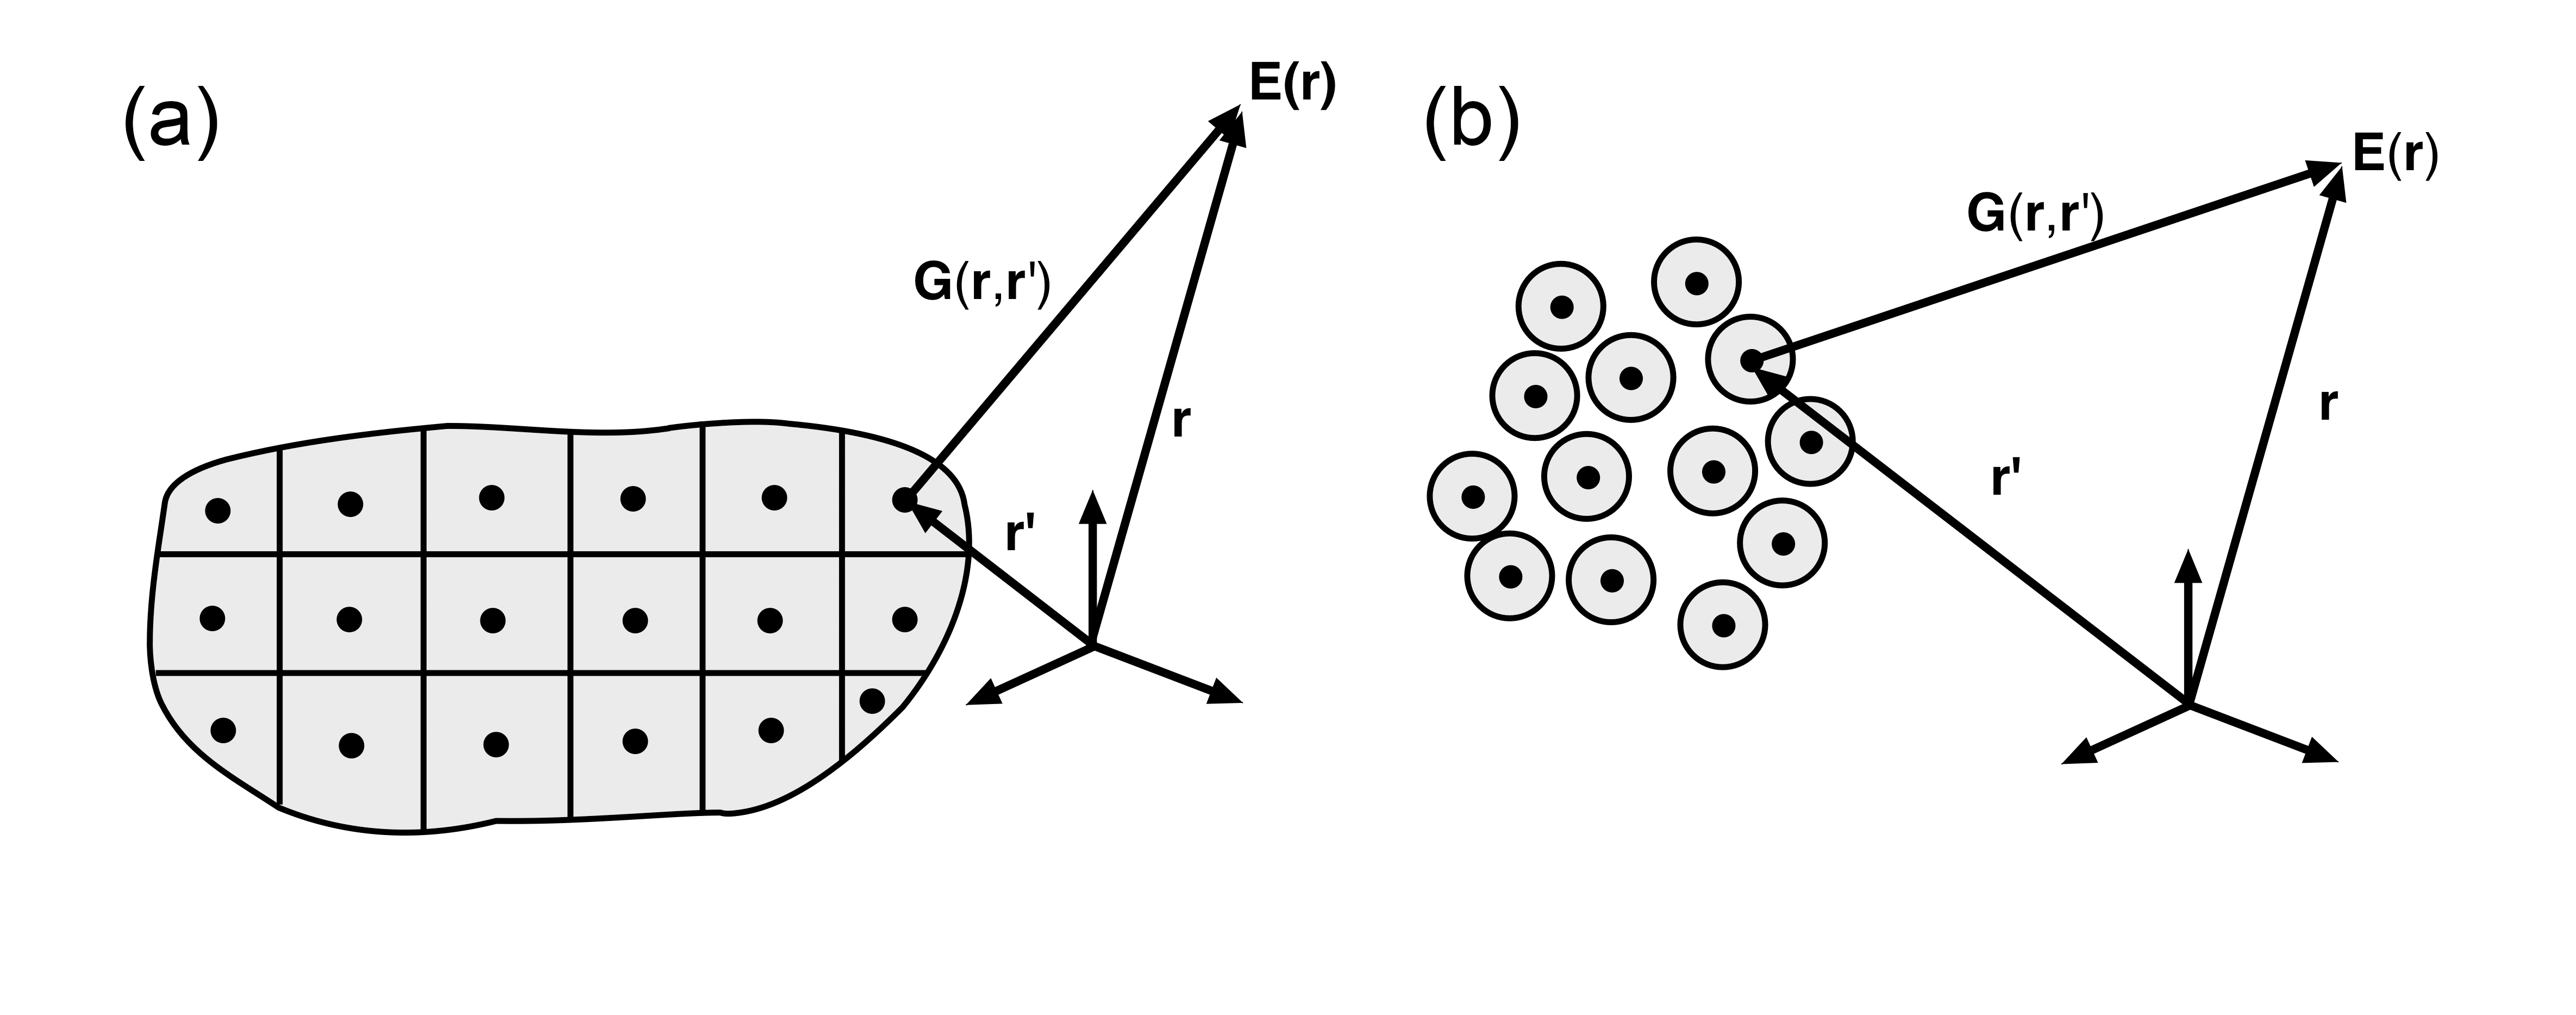
\includegraphics[width=10cm]{chapter_2/figures/DDA.png} 
\par\end{centering}
\caption{Schematic representation of: (a) a discretised object into dipoles (black points); (b) a random systems where each particle is described by a single dipole. The electric field $\mathbf{E}$ at point $\mathbf{r}$, in both situations, is obtained from the sum of the field from each dipole. \label{fig:chap2_DDA_scheme}}
\end{figure}
For a set of $\mathcal{N}$ dipoles which form a system, the excitation field over each dipole can be obtained by considering Eq. (\ref{eq:lipschw}) in the discrete form:

\begin{equation}
\mathbf{E}_{i} =  \mathbf{E}_{0}\left(\mathbf{r}_i,\omega\right) + \frac{k^2}{\epsilon_{0}}\sum_{i\neq j}{\mathbf{G}\left(\mathbf{r}_i,\mathbf{r}_j,\omega\right)}\epsilon_{0}\boldsymbol{\alpha}\mathbf{E}_{j},\label{eq:chap2_DDA}
\end{equation}
where $\mathbf{p}_i=\epsilon_{0}\boldsymbol{\alpha}\mathbf{E}_i$ is the induced dipole moment or the polarisation\footnote{We describe the polarisation of particles in chapter (\ref{chap2:pol_of_small_particles}).} of the $i-$element. Eq. (\ref{eq:chap2_DDA}) is a set of $3\mathcal{N}$ linear equations with $3\mathcal{N}$ unknowns, representing the exciting fields at the scatterer's position. Solving the system of equations, it is possible to know the polarisation of each dipole, which in turn allows us to obtain the electric field at any position in the space:

\begin{equation}
\mathbf{E}\left(\mathbf{r},\omega\right) =  \mathbf{E}_{0}\left(\mathbf{r},\omega\right) + \frac{k^2}{\epsilon_{0}}\sum_{i=1}^{\mathcal{N}}{\mathbf{G}\left(\mathbf{r},\mathbf{r}_{i},\omega\right)}\epsilon_{0}\boldsymbol{\alpha}\mathbf{E}_{i}.
\end{equation}

\section{Polarisability of small particles\label{sec:Pol_small_part}}

The result of light interaction with matter depends not only of light properties (frequency, intensity, etc.) but also the matter properties (dielectric response, shape, etc.).\\
This section is devoted to the study of the electromagnetic response of small particles, when compared with the incident wavelength, when illuminated. 
Small particles get polarised when excited, exhibiting an induced dipole. This behaviour allow us to regard each particle as a new source of radiation, commonly referred as a secondary source (see Sec. \ref{sec:Wave_scatt_small_part}). 

Let us consider a small particle in vacuum with volume $V$ and with dielectric tensor $\boldsymbol{\epsilon}\left(\omega\right)$. The particle is positioned at $\mathbf{r}_p$ and the incident electric field that excites the particle is $\mathbf{E}_{0}\left(\omega\right)$. The polarisability $\boldsymbol{\alpha}$ of the particle relates the incident electric field $\mathbf{E}_{0}\left(\omega\right)$ with the polarisation $\mathbf{p}\left(\omega\right)$. Mathematically, can be represented as:

\begin{equation}
\mathbf{p}\left(\omega\right) = \epsilon_{0}\boldsymbol{\alpha}\left(\omega\right) \mathbf{E}_{0}\left(\omega\right).
\end{equation}

The polarisability takes into account the shape and dimensions as well as the electromagnetic response of the particle material. Its anisotropic nature implies that the induced dipole can have an orientation which is different from the incident electric field.
% a different orientation of the incident electric field. 
In the following subsection we calculate the polarisability for small anisotropic spherical particles.

\subsection{Polarisability of small anisotropic spherical particles\label{chap2:pol_of_small_particles}}

Let us consider a single spherical particle with radius $a$, much smaller than the wavelength, where the electric field does not vary inside of its volume. \\
From the Lippmann-Schwinger equation, we can approximate the total electric field for a point $\mathbf{r}$ outside of the particle:

\begin{equation}
\mathbf{E}\left(\mathbf{r}\right) \approx \mathbf{E}_{0}\left(\mathbf{r}\right) + k^{2}\left[\boldsymbol{\epsilon}-\mathbb{I}\right]V\mathbf{G}\left(\mathbf{r},\mathbf{r}_{p}\right)\mathbf{E}_{ins}\label{eq:chap2:E_tot_comp},
\end{equation}
where $\mathbf{E}_{ins}$ is the electric field inside the particle. Because the particle is the only scatterer present in the system, the electric field that illuminates the particle is $\mathbf{E}_{0}\left(\mathbf{r}_{p}\right)$. The particle's dipole can be written as:

\begin{equation}
\mathbf{p}=\epsilon_0\boldsymbol{\alpha}\mathbf{E}_{0}\left(\mathbf{r}_{p}\right).
\end{equation}
Eq. (\ref{eq:chap2:E_tot_comp}) can be rewritten in a more compact way:

\begin{equation}
\mathbf{E}\left(\mathbf{r}\right) \approx \mathbf{E}_{0}\left(\mathbf{r}\right) + \frac{k^2}{\epsilon_{0}}\mathbf{G}\left(\mathbf{r},\mathbf{r}_{p}\right)\mathbf{p}.
\end{equation}
In this approximation we can use Eq. (\ref{eq:lipschw}) to obtain the self-consistent solution for $\mathbf{E}_{ins}$:

\begin{eqnarray}
\mathbf{E}_{ins} & = & \mathbf{E}_{0}\left(\mathbf{r}_{p}\right)+k^{2}\left[\boldsymbol{\epsilon}-\mathbb{I}\right]\left(\int \mathbf{G}\left(\mathbf{r},\mathbf{r}_{p}\right)dV'\right)\cdot\mathbf{E}_{ins}\nonumber \\
 & = & \mathbf{E}_{0}\left(\mathbf{r}_{p}\right)+k^2\left[\boldsymbol{\epsilon}-\mathbb{I}\right]V\left<\mathbf{G}\right>\cdot\mathbf{E}_{ins},
\end{eqnarray}
where $\left<\mathbf{G}\right>$  is the average value of the Green tensor in the volume of the particle $V$ which came from the volume integral.\\
The internal self-consistent field is given by:

\begin{equation}
\mathbf{E}_{ins} = \left\{\mathbb{I}-k^2V\left<\mathbf{G}\right>\left[\boldsymbol{\epsilon}-\mathbb{I}\right]\right\}^{-1}\mathbf{E}_{0}\left(\mathbf{r}_{p}\right).
\end{equation}

For small spherical particles, the average Green tensor is given by \cite{Bladel_1961, Yaghjian_1980,Wang_1991,Carminati_2006}:

\begin{equation}
\lim_{v\rightarrow 0}\left<\mathbf{G}\right>\simeq \left(-\frac{1}{3k^2V}+i\frac{k}{6\pi}\right)\mathbb{I},
\end{equation}
where $\Im\left\{\mathbf{G}\left(0\right)\right\}=\frac{k}{6\pi}\mathbb{I}$.
So, we have:

\begin{equation}
\mathbf{E}_{ins} = \left[\mathbb{I}+\left(\frac{1}{3}-\frac{ik^3V}{6\pi}\right)\mathbb{I}\left(\boldsymbol{\epsilon}+2\mathbb{I}\right)\right]^{-1}\mathbf{E}_{0}\left(\mathbf{r}_{p}\right).
\end{equation}


Defining $\boldsymbol{\alpha}_0 = 3V\left\{\boldsymbol{\epsilon}-\mathbb{I}\right\}\left\{\boldsymbol{\epsilon}+2\mathbb{I}\right\}^{-1}$ as the static polarisability, it is possible to express the field inside as:

\begin{equation}
\mathbf{E}_{ins}=3\left(\boldsymbol{\epsilon}+2\mathbb{I}\right)^{-1}\left\{\mathbb{I}-i\frac{k^3}{6\pi}\boldsymbol{\alpha}_{0}\right\}^{-1}\mathbf{E}_{0}\left(\mathbf{r}_{p}\right).\label{eq:field_inside_particle}
\end{equation}
The total field outside of the particle can be expressed as:

\begin{eqnarray}
\mathbf{E}\left(\mathbf{r}\right) & = & \mathbf{E}_{0}\left(\mathbf{r}\right)+k^{2}\int\mathbf{G}\left(\mathbf{r},\mathbf{r}_{p}\right)\left(\boldsymbol{\epsilon}-\mathbb{I}\right)\mathbf{E}\left(\mathbf{r}'\right)dV' \nonumber \\
 & = & \mathbf{E}_{0}\left(\mathbf{r}\right)+k^{2}V\mathbf{G}\left(\mathbf{r},\mathbf{r}_{p}\right)\left(\boldsymbol{\epsilon}-\mathbb{I}\right)\mathbf{E}_{ins}\nonumber \\
 & = & \mathbf{E}_{0}\left(\mathbf{r}\right)+k^{2}V\mathbf{G}\left(\mathbf{r},\mathbf{r}_{p}\right)\left(\boldsymbol{\epsilon}-\mathbb{I}\right)3\left(\boldsymbol{\epsilon}+2\mathbb{I}\right)^{-1}\left\{\mathbb{I}-i\frac{k^3}{6\pi}\boldsymbol{\alpha}_{0}\right\}^{-1}\mathbf{E}_{0}\left(\mathbf{r}_{p}\right)\nonumber\\
 & = & \mathbf{E}_{0}\left(\mathbf{r}\right) + \frac{k^2}{\epsilon_{0}}\mathbf{G}\left(\mathbf{r},\mathbf{r}_{p}\right)\cdot \mathbf{p} \label{eq:chap2_poleq2}.
\end{eqnarray}
The induced dipole  $\mathbf{p}$ is obtained from the previous equations:

\begin{equation}
\boldsymbol{\alpha}\mathbf{E}_{0}\left(\mathbf{r}_{p}\right) = V\left(\boldsymbol{\epsilon}-\mathbb{I}\right)3\left(\boldsymbol{\epsilon}+2\mathbb{I}\right)^{-1}\left\{\mathbb{I}-i\frac{k^3}{6\pi}\boldsymbol{\alpha}_{0}\right\}^{-1}\mathbf{E}_{0}\left(\mathbf{r}_{p}\right),
\end{equation}
Substituting $\boldsymbol{\alpha}_0= 3V\left(\boldsymbol{\epsilon}-\mathbb{I}\right)\left(\boldsymbol{\epsilon}+2\mathbb{I}\right)^{-1}$ we obtain:

\begin{equation}
\boldsymbol{\alpha}=\boldsymbol{\alpha}_{0}\left\{\mathbb{I}-i\frac{k^3}{6\pi}\boldsymbol{\alpha}_{0}\right\}^{-1}\label{eq:chap2_radiative_correction}.
\end{equation}
Eq. (\ref{eq:chap2_radiative_correction}) is the expression of the polarisability with the radiative correction, that is valid for any permittivity tensor $\boldsymbol{\epsilon}$.

\subsection{Polarisability of resonant particles\label{sec:chap2_resonant}}

Resonant point dipoles are special particles because they have the ability of maximise the scattering of light. Is frequently used in theoretical models where phenomena are critical with the amount of scattering.\\
For a resonant particle, is considered a diagonal dielectric tensor only with real part, \textit{i.e.}, without absorption, where the static polarisability is maximum. The diagonal elements of the dielectric tensor assume the value of $\epsilon = -2$ for a given frequency. Thus, the resonant polarisability with radiative corrections for a spherical particle is given by:

\begin{equation}
\alpha_{res} = i\frac{6\pi}{k^3}.
\end{equation}

\subsection{Absorption of small particles\label{sec:chap2_abs_small_part}}

When light is incident over a particle, a fraction of the incident beam can be absorbed and transformed into internal energy, usually in thermal energy \cite{Baffou_2009}.
In this section we evaluate the absorbed power by a small particle.\\
The mean of energy absorbed, over a period, within the volume $V$ is given by:

\begin{equation}
\left<\frac{dW_{abs}}{dt}\right>=\frac{1}{2}\int_{V}\Re\left\{\mathbf{j}^{*}\cdot\mathbf{E}_{ins}\right\}dV,\label{eq:mean_energy_absorbed}
\end{equation}
where $\mathbf{j}=-i\omega \mathbf{p}\delta\left(\mathbf{r}-\mathbf{r}'\right)$ is the current induced by the field inside the particle $\mathbf{E}_{ins}$. Eq. (\ref{eq:mean_energy_absorbed}) can be written as:

\begin{equation}
\left<\frac{dW_{abs}}{dt}\right>=P_{abs}=-\frac{\omega}{2} \Im\left\{\mathbf{p}^{*}\cdot\mathbf{E}_{ins}\right\}.
\end{equation}
The electric field inside of the particle is defined by Eq. (\ref{eq:field_inside_particle}) and the dipole moment of the particle can be expressed as:

\begin{equation}
\mathbf{p} = V\epsilon_{0}\left(\boldsymbol{\epsilon}-\mathbb{I}\right)\cdot\mathbf{E}_{ins},
\end{equation}
where can we get the absorbed power by the particle:

\begin{equation}
P_{abs} = -V\frac{\omega \epsilon_0}{2}\Im{\left\{\left(\boldsymbol{\epsilon}\cdot\mathbf{E}_{ins}\right)^{*}\cdot\mathbf{E}_{ins}\right\}}.\label{eq:abs_gen}
\end{equation}
For the special case where the dielectric tensor is diagonal, $\boldsymbol{\epsilon}=\epsilon\mathbb{I}$, Eq. (\ref{eq:abs_gen}) can be simplified:

\begin{equation}
P_{abs} = V\frac{\omega \epsilon_0}{2}\Im{\left\{\epsilon\right\}}\left|\mathbf{E}_{ins}\right|^2.\label{eq:Pabs_diel_cnst}
\end{equation}
To obtain the expression involving the polarisability, we substitute Eq. (\ref{eq:field_inside_particle}) into Eq. (\ref{eq:Pabs_diel_cnst}):

\begin{equation}
P_{abs} = 3V\frac{\omega \epsilon_{0}}{2}\frac{3\Im\left(\epsilon\right)}{\left|\epsilon+2\right|^2}\left|1-i\frac{k^3}{6\pi}3V\frac{\epsilon-1}{\epsilon + 2}\right|^{-2}\left|\mathbf{E}_{0}\left(\mathbf{r}_{p}\right)\right|^2.\label{eq:abs_eps_cst2}
\end{equation}
Considering the identity $ \frac{3\Im{\left(\epsilon\right)}}{\left|\epsilon+2\right|^2}=\Im{\left(\frac{\epsilon-1}{\epsilon + 2}\right)}$, we can rewrite Eq. (\ref{eq:abs_eps_cst2}):

\begin{equation}
P_{abs}= \frac{\omega\epsilon_0}{2}\frac{\Im{\left(\alpha_{0}\right)}}{\left|1-ik^3/\left(6\pi\right)\alpha_0\right|^2}\left|\mathbf{E}_{0}\left(\mathbf{r}_{p}\right)\right|^2,
\end{equation}
and the polarisability equation can be written as:

\begin{equation}
\frac{\Im{\left(\alpha_{0}\right)}}{\left|1-ik^3/\left(6\pi\right)\alpha_0\right|^2}=\Im{\left(\alpha\right)}-\frac{k^3}{6\pi}\left|\alpha\right|^2,
\end{equation}
or considering Eq. (\ref{eq:chap2_radiative_correction}), the absorbed power can be expressed as:

\begin{equation}
P_{abs} = \frac{\omega\epsilon}{2}\left(\Im{\left(\alpha\right)}-\frac{k^3}{6\pi}\left|\alpha\right|^2\right)\left|\mathbf{E}_{0}\left(\mathbf{r}_{p}\right)\right|^2.
\end{equation}

For a non-absorbing particle, $\Im\left(\alpha\right)=\frac{k^3}{6\pi}\left|\alpha\right|^2$, which is a form of the optical theorem.

\section{Dielectric tensor\label{sec:chap2_dielectric_tensor}}

The influence of an electric field $\mathbf{E}$ over a material is represented by the electric displacement field $\mathbf{D}$, that characterises the electron organisation in the material, the changes migration and electric dipole orientation. Both fields are related through the dielectric tensor:

\begin{equation}
\mathbf{D} = \boldsymbol{\epsilon}\mathbf{E}.
\end{equation}
A material characterised by a diagonal tensor, when in the presence of a magnetic field, becomes asymmetric. Materials with this behaviour are magneto-optical materials and are a primary topic in this thesis. The elements of the tensor are dependent of the magnetic field, $\epsilon_{ij}\left(H\right)=\epsilon_{ji}\left(-H\right)$, and the tensor reads:

\begin{equation}
\boldsymbol{\epsilon} = \left(\begin{array}{ccc}
\epsilon_{xx} & \epsilon_{xy} & \epsilon_{xz}\\
-\epsilon_{xy} & \epsilon_{yy} & -\epsilon_{yz}\\
-\epsilon_{xz} & \epsilon_{yz} & \epsilon_{zz}
\end{array}\right),
\end{equation}
where $\epsilon_{ii}$ represents the optical properties of the materials and $\epsilon_{ij}$ the magneto-optical properties. The elements of the dielectric tensor can be described as \cite{sepulveda2003linear}:

\begin{equation}
\epsilon_{ij} = \epsilon_{ij}^{0}+\sum_{k}a_{ijk}H_{k}+\sum_{k}\sum_{l}b_{ijkl}H_{k}H_{l}+...,
\end{equation}
with $\epsilon_{ij}^{0}$ the dielectric constants in absence of the magnetic field, $a_{ijk}$ the coefficients of the third rank order and $b_{ijkl}$ the coefficients of fourth rank that describes the linear and quadratic dependence respectively with the magnetic field $H_{i}$. We should note that for ferromagnetic materials the dielectric tensor depends on the material magnetisation $M_{i}$ instead of the magnetic field. Since the small relevance of the quadratic elements, we only consider the linear dependence with the magnetic field. So, the dielectric tensor adopts the form:

\begin{equation}
\boldsymbol{\epsilon} = \left(\begin{array}{ccc}
\epsilon & aH_{z} & aH_{y}\\
-aH_{z} & \epsilon & -aH_{x}\\
-aH_{z} & aH_{x} & \epsilon
\end{array}\right).
\end{equation}
The dielectric tensor form is strongly dependent of the relative orientation of the applied magnetic field. For example, when the applied magnetic field is perpendicularly aligned with the sample plane, as shown in Fig. (\ref{fig:chap2_kerr_config})(a), the dielectric tensor assumes the form:

\begin{equation}
\boldsymbol{\epsilon} = \left(\begin{array}{ccc}
\epsilon & aH_{z} & 0\\
-aH_{z} & \epsilon & 0\\
0 & 0 & \epsilon
\end{array}\right),
\end{equation}

that corresponds to the polar Kerr configuration \cite{armelles2013magnetoplasmonics}, where the $x-$ and  $y-$ components are coupled. A direct consequence of the tensor form is the conversion of the $x-$polarisation into $y-$polarisation when an incident beam is reflected through the scatterer. To evaluate the conversion, two magnitudes are used: the magnetic field induced rotation, $\theta$, and the elliptically, $\phi$. These two numbers constitute the magneto-optical activity magnitude:

\begin{equation}
\Phi=\theta+i\phi.
\end{equation}
There are three possible magneto-optical configurations, that are defined by the relative orientation between the magnetic field and the plane of incidence: the polar, longitudinal and transversal configurations. These are schematically represented if  Fig. (\ref{fig:chap2_kerr_config}).

\begin{figure}[h]
\begin{centering}
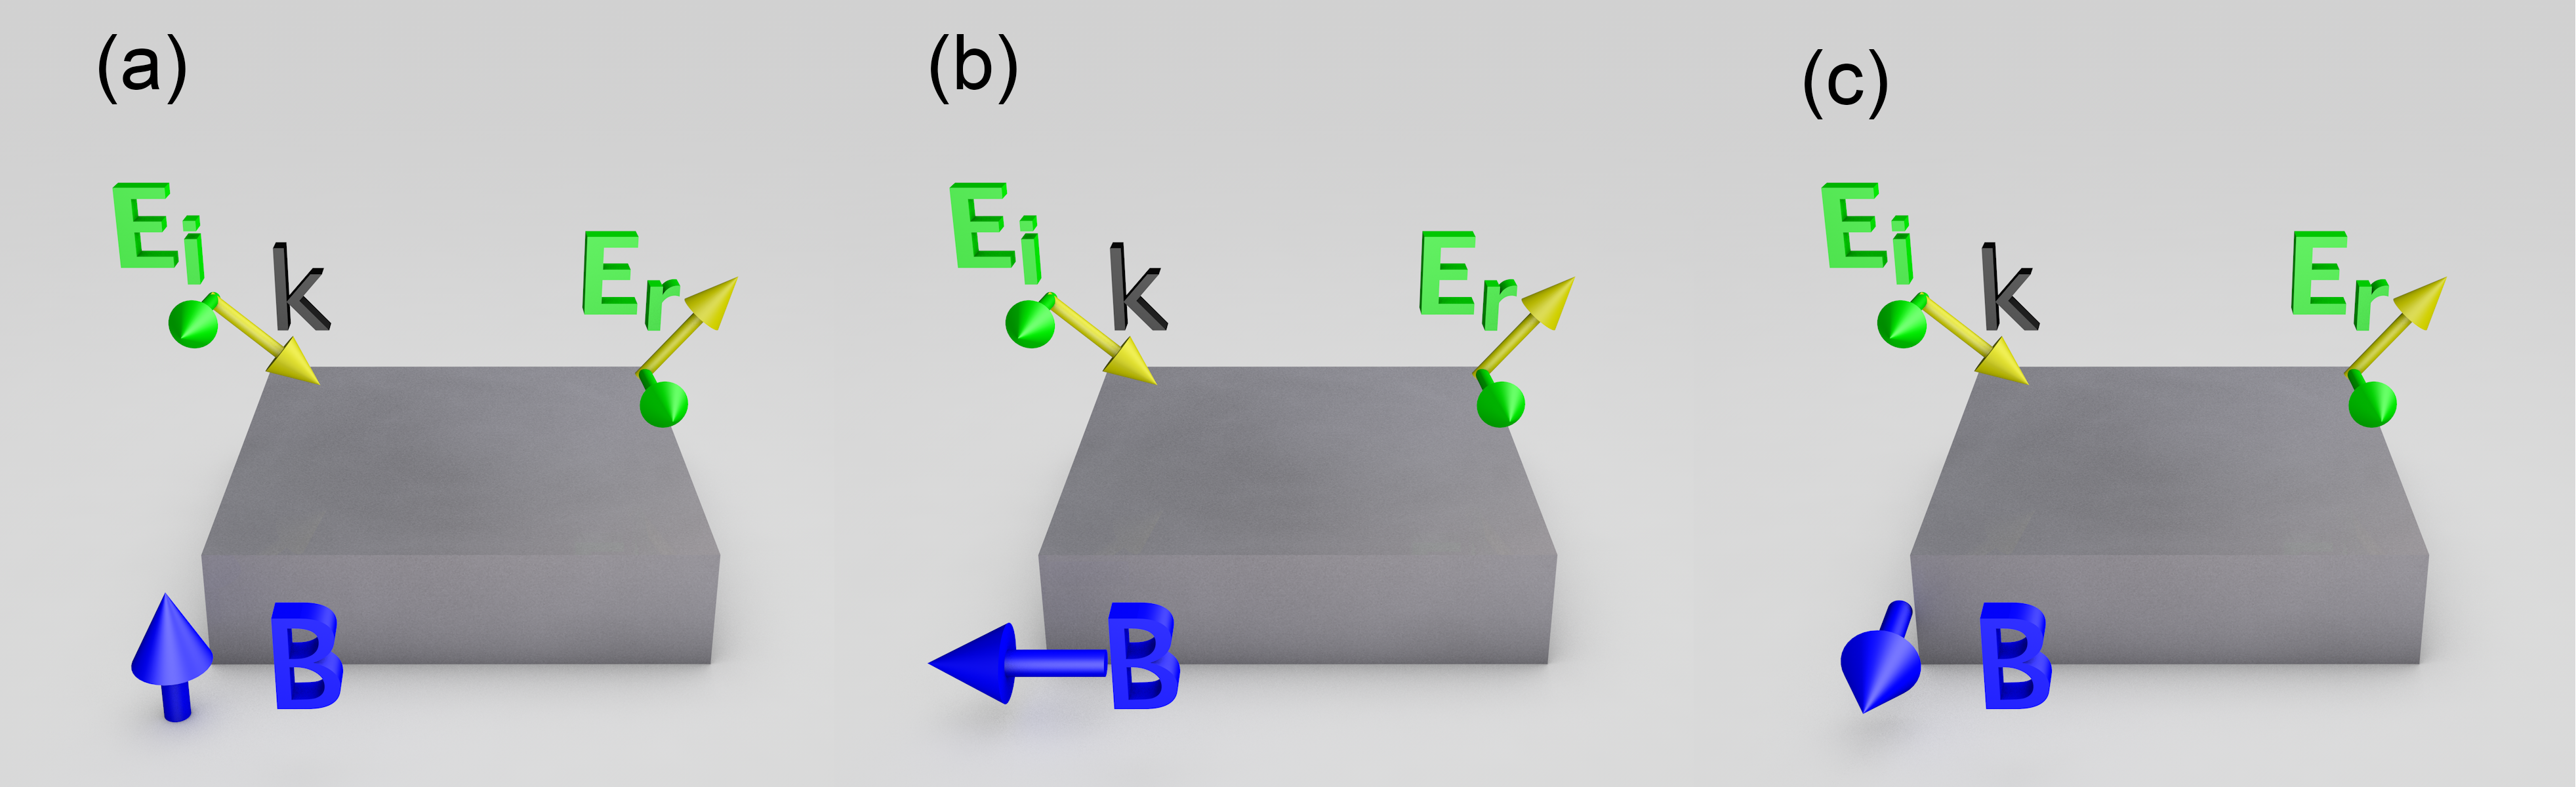
\includegraphics[width=12cm]{chapter_2/figures/kerr_configurations.png} 
\par\end{centering}
\caption{Schematic representation of the magneto-optical Kerr effect. In configuration: (a) is represented the polar configuration; (b) the longitudinal configuration; and (c) the transversal configuration. Each configuration is defined by the relative orientation between the magnetic field and the plane of incidence. \label{fig:chap2_kerr_config}}
\end{figure}



\section{Dipole radiation\label{chap2:Dipole_radiation}}

%In nature, many different types of structures, like atoms, molecules or quantum dots to name a few, radiate like dipoles. Such structures can be modelled as three level systems, with $\ket{e_{1}}$ and $\ket{e_{2}}$ two unstable vibrational levels of an excited electronic state and $\ket{g}$ the ground state. The system is excited with radiation at frequency $\omega_{e_{1}}$ to state $\ket{e_{1}}$ and instantly decay to the $\ket{e_{2}}$ state. At this point, it takes a time $\tau$ (lifetime) to jump to the fundamental state $\ket{g}$. This transition is followed by the emission of a photon at frequency $\omega_{e_{2}}$, called fluorescent frequency. \\

%\subsection{Purcell effect}

Since Purcell work in 1946 \cite{Purcell_1946}, it is known that the decay rate $\gamma$ (and consequently the lifetime $\gamma=\frac{1}{\tau}$) of an emitter is not only function of the intrinsic properties of atoms and molecules, but also of the environment where the emitter is placed.\\ 
 This phenomenon has been observed in emitters placed close to planar interfaces \cite{Drexhage_1966} and cavities \citep{Goy_1983}. Also it was theoretically predicted \cite{yablonovitch1987inhibited} and experimentally verified in two \cite{Kress_2005, Englund_2005} and three dimensional photonic crystals \cite{Lodahl_2004} and more recently in plasmonic \cite{Carminati_2006, Castanie_2012_distance, esteban2014strong} and magnetoplasmonic structures \cite{Nikolova_2013}.\\
A first approach to the understanding of this phenomenon can be made by evaluation the power radiated by an emitter when it is placed in different environments. Usually the modification of the radiated power is compared with the radiated power of the emitter in vacuum, \textit{i.e.}, in the absence of any scattering object.\\
In the following subsections we give a introduction to the analytical techniques to evaluate the radiated power, starting by calculate in free space and then in the presence of an inhomogeneous environment.

\subsection{Radiation in free space}

In the electromagnetic field, the representation of the energy flux density is given by the Poynting vector $\mathbf{S}$. This vector carries the information about the direction of propagation of the electromagnetic energy and is mathematically defined by:
\begin{equation}
\mathbf{S}\left(t\right)=\mathbf{E}\left(t\right)\times\mathbf{H}\left(t\right),
\end{equation} 
where the electric and magnetic field are in the time domain. For an electric point dipole $\boldsymbol{\mu}$, the radiated power can be determined by integrating the Poynting vector $\mathbf{S}\left(t\right)$ over a infinitesimally closed surface that surrounds the source. The average radiated power for an harmonically oscillating dipole is:

\begin{equation}
P_{0}=\frac{\left|\mathbf{\boldsymbol{\mu}}\right|^2}{4\pi\epsilon_{0}}\frac{k^4c}{3}.
\end{equation}
This equation indicates that the radiated power is proportional to the fourth power of the wavenumber.\\
An alternative way of evaluate the radiated power of a dipole in free space is presented in Appendix (\ref{App:eval_green_source}).
%As alternative, it could be calculated by integrating the time averaged P.

\subsection{Dipole radiation in inhomogeneous environments: \\ method I \label{subch:Dip_inh_envi}}

The behaviour of a dipole emitter embedded in an inhomogeneous environment can be characterised by the emitter radiated power. According with Poynting's theorem \cite{Jackson_CE}, the radiated power of a time harmonic current distribution is identical to the rate of energy dissipation:

\begin{equation}
\frac{dW}{dt}=-\frac{1}{2}\int_V^{} \Re\left\{\mathbf{j}^{*}\cdot\mathbf{E}\right\} dV.
\end{equation}
where $\mathbf{j}$ is not the total current density but instead represents the source current that generates the fields or the loss currents corresponding to the thermal losses and $V$ is the volume of the current distribution. If we consider the source like the one described in Eq. (\ref{eq:EM_source}), we obtain:


\begin{equation}
\left<\frac{dW}{dt}\right>=\frac{\omega}{2} \Im\left\{\boldsymbol{\mu}^{*}\cdot\mathbf{E}\left(\mathbf{r}_{0}\right)\right\},\label{eq:Radiated_power}
\end{equation}
being $\mathbf{E}\left(\mathbf{r}_{0}\right)$ the electric field at dipole position at $\mathbf{r}_0$.\\
In an inhomogeneous environment the field at dipole position $\mathbf{E}\left(\mathbf{r}_{0}\right)$ can be separated in two components. One is the dipole field in its own position $\mathbf{E}_{0}\left(\mathbf{r}_0\right)$ and the other is the scattered field  $\mathbf{E}_{s}\left(\mathbf{r}_0\right)$ by the surrounding environment. This can be expressed as:

\begin{equation}
\mathbf{E}\left(\mathbf{r}_{0}\right) = \mathbf{E}_{0}\left(\mathbf{r}_{0}\right) + \mathbf{E}_{s}\left(\mathbf{r}_{0}\right). \label{eq:E_source_inh}
\end{equation}
The total radiated power by the emitter can be evaluated by integrating the Poynting vector over the infinitesimal surface that surrounds the source. An alternative is to evaluate Eq. (\ref{eq:Radiated_power}) with an adequate field like Eq. (\ref{eq:E_source_inh}), \textit{i.e.}, the total electric field at the emitter position.\\
So, the total power radiated can be written as:

\begin{equation}
P_{tot}=\frac{\left|\mathbf{\boldsymbol{\mu}}\right|^2}{4\pi\epsilon_{0}}\frac{k^4c}{3} + \frac{kc}{2}\Im\left\{{\boldsymbol{\mu}^{*}\cdot \mathbf{E}_{s}\left(\mathbf{r}_{0}\right)}\right\}, 
\end{equation}
or normalized by the radiated power in free space:

\begin{equation}
\frac{P_{tot}}{P_{0}}=1 + \frac{6\pi\epsilon_{0}}{k^{3}\left|\boldsymbol{\mu}\right|^2}\Im\left\{{\boldsymbol{\mu}^{*}\cdot \mathbf{E}_{s}\left(\mathbf{r}_{0}\right)}\right\}\label{eq:norm_decay_rate}.
\end{equation}
From this equation we can see that the modification of the radiated power only depends of the scattered field, \textit{i.e.}, the field that returns after interfering with surroundings.

\subsection{Dipole radiation in inhomogeneous environments: \\ method II}

In an inhomogeneous environment like represented in Fig. (\ref{fig:inh_envir}), we can calculate the radiated power by an emitter in an alternative way to the one presented in Sec. (\ref{subch:Dip_inh_envi}).\\
The total radiated power by an emitter is obtained by evaluation of the radiated power in far field, which is called radiative power, and the absorbed power by the inhomogeneous environment. The first one, the radiated power in far field takes into account all the fields generated by the principal and secondary sources, formed by the emitter and the scattering particles respectively. The second one, the absorbed radiation by the inhomogeneous environment can be calculated by evaluating the absorbed power for all particles, like discussed in Sec. (\ref{sec:chap2_abs_small_part}). \\
Thus, due to the energy conservation:

\begin{equation}
P_{tot} = P_{rad} + P_{abs},
\end{equation}
where $P_{tot}$ is the total radiated power by the emitter, $P_{rad}$ is the radiated power by the entire system in far field and $P_{abs}$ the absorbed power by the environment. 

\begin{figure}[h]
\begin{centering}
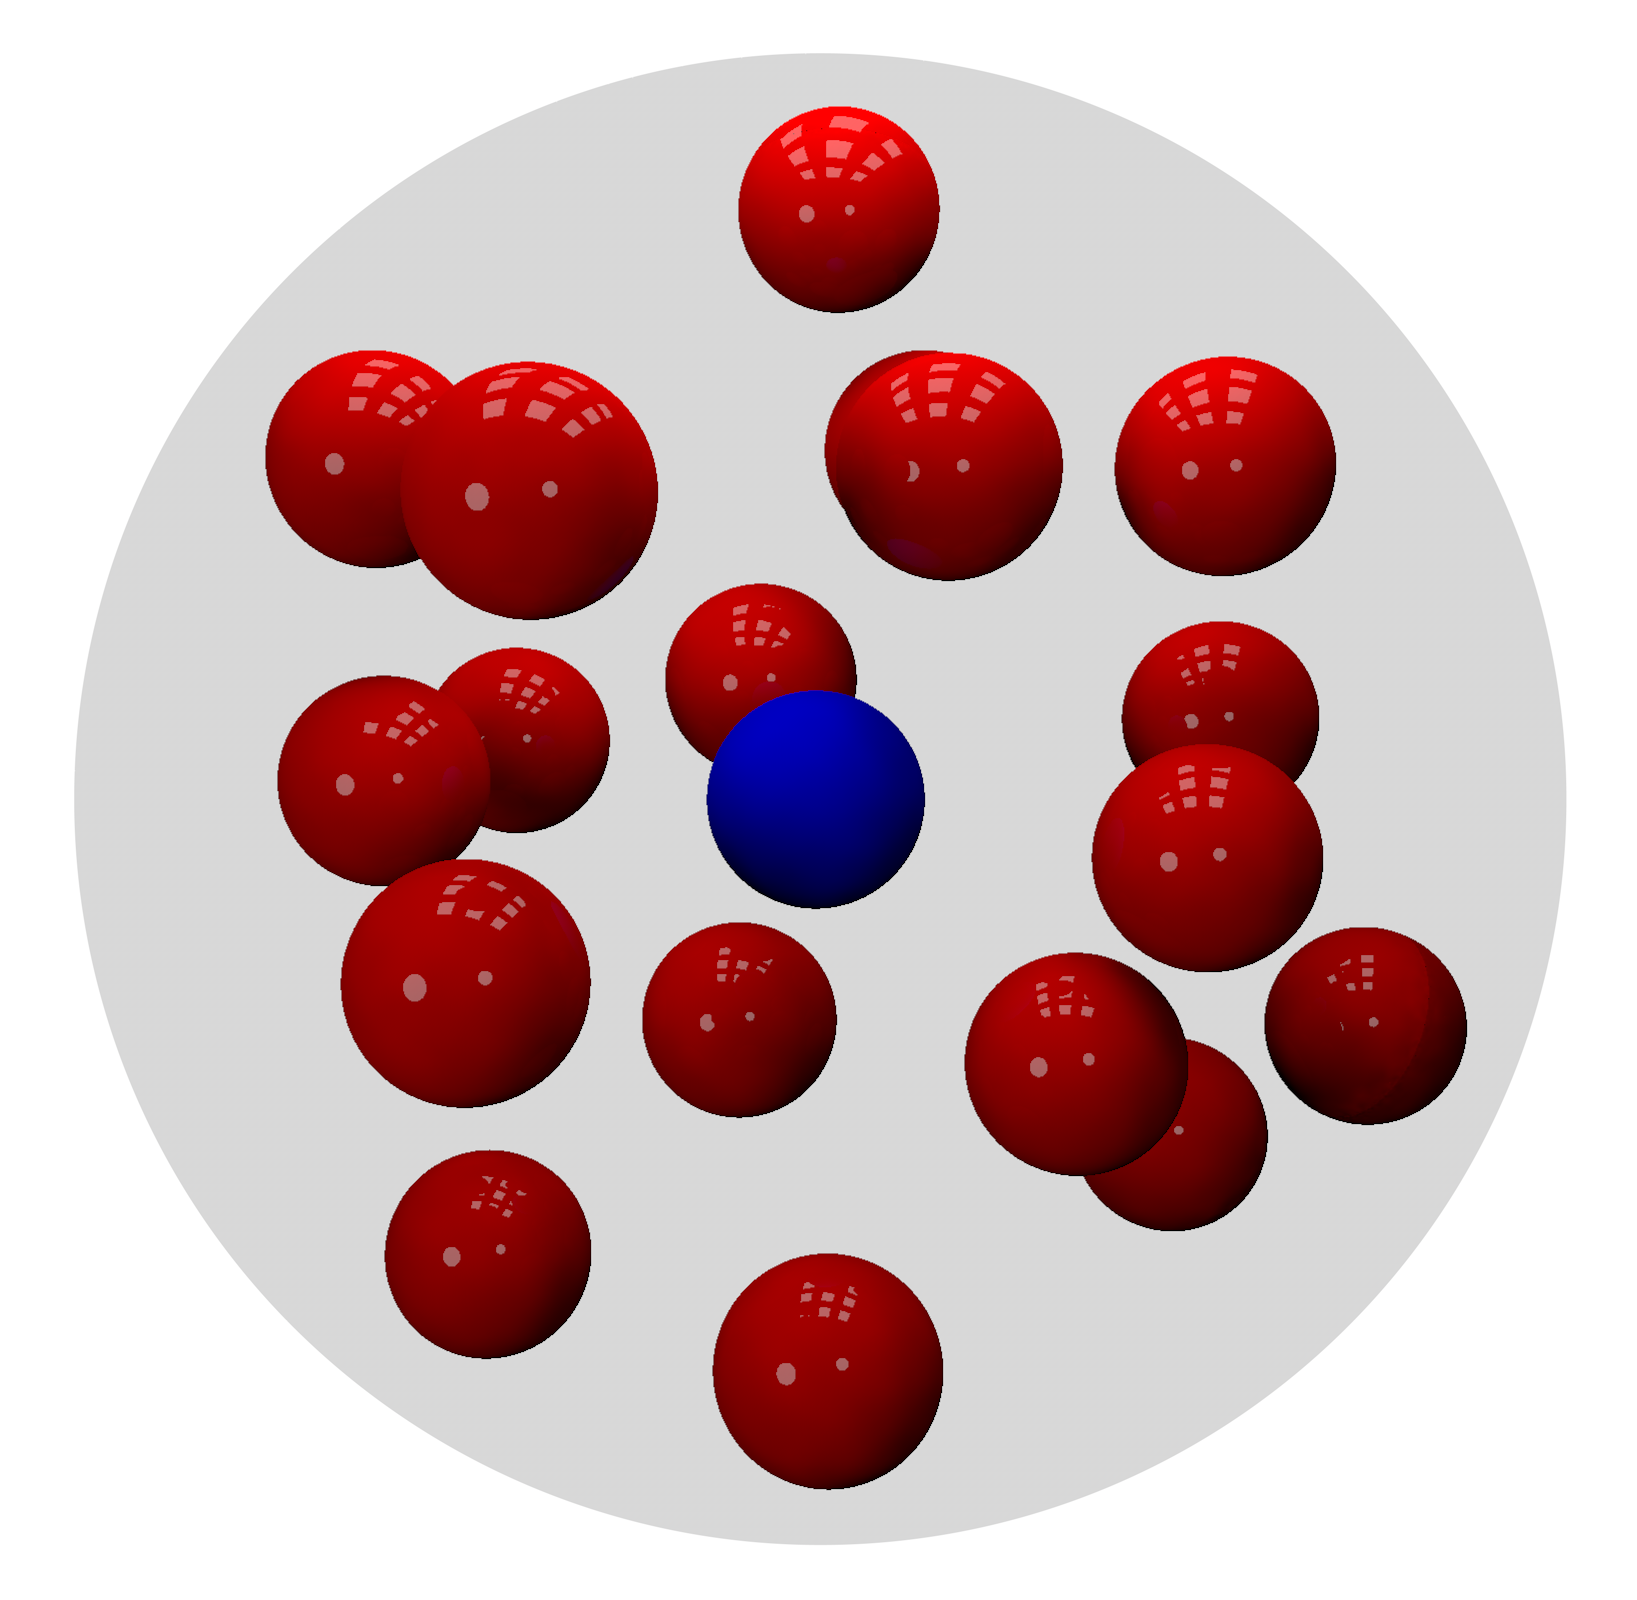
\includegraphics[width=6cm]{chapter_2/figures/inh_envirnm.png} 
\par\end{centering}
\caption{Schematic representation of an emitter $\boldsymbol{\mu}$ (blue sphere) in an inhomogeneous environment (represented by red spheres). The transparent sphere represents the shell that involves the entire system in far field.\label{fig:inh_envir}}
\end{figure}


Let us consider an emitter $\boldsymbol{\mu}$ located at $\mathbf{r} = \mathbf{r}_{0}$ surrounded by $\mathcal{N}$ dipolar particles $\mathbf{p}_n$ located at $\mathbf{r} = \mathbf{r}_{n}$ ($n = 1,...,\mathcal{N}$).

Considering the superposition principle, the total field at position $\mathbf{r}$ is given by:

\begin{equation}
\mathbf{E}\left(\mathbf{r}\right) = \frac{k^2}{\epsilon_{0}}\left[\mathbf{G}\left(\mathbf{r},\mathbf{r}_{0}\right)\cdot \boldsymbol{\mu} + \sum_{n=1}^{\mathcal{N}}\mathbf{G}\left(\mathbf{r},\mathbf{r}_{n}\right)\cdot \mathbf{p}_{n} \right].
\end{equation}

In far field, \textit{i.e.}, making the asymptotic expansion of the Green tensor $R = \left|\mathbf{r}\right| \gg \left|\mathbf{r}_{n}\right|$, and $\mathbf{k}$ the wave vector defined by $\mathbf{k}=k \mathbf{u}_{r}$ with $\mathbf{u}_{r}={\mathbf{r}}/{\left|\mathbf{r}\right|}$, the electric and magnetic field can be written as:

\begin{eqnarray}
\mathbf{E}_{n}\left(\mathbf{r}\right) & = & \frac{k^{2}}{\epsilon_{0}}\mathbf{G}\left(\mathbf{r},\mathbf{r}_{n}\right)\cdot\mathbf{p}_{n}\approx\frac{e^{ikR}}{4\pi\epsilon_{0}} R \left\{ \left(\mathbf{k}\times\mathbf{p}_{n}\right)\times\mathbf{k}\right\} e^{-i\mathbf{k}\cdot\mathbf{r}_{n}}\\
\mathbf{H}_{n}\left(\mathbf{r}\right) & = & \frac{1}{k}\sqrt{\frac{\epsilon_{0}}{\mu_{0}}}\left(\mathbf{k}\times\mathbf{E}_{n}\right).
\end{eqnarray}


With the electric and magnetic field is defined the Poynting vector. Integrating over a spherical surface that contains the entire system (see App. (\ref{App1:eval_dip_inh_env})), the total radiated power will be given by:
\begin{equation}
P = \frac{k^3}{2}\frac{1}{\epsilon_{0}\sqrt{\epsilon_{0} \mu_{0}}} \sum_{mn}\Re \left\{ \mathbf{p}_{m}^{*}\cdot \Im \left[ \mathbf{G} \left(\mathbf{r}_{m},\mathbf{r}_{n}\right)\right]\cdot \mathbf{p}_{n} \right\}.
\end{equation} 


\subsection{Local Density of states (LDOS)}

When an emitter is embedded in an inhomogeneous environment, the radiated power is a function of its position, orientation and frequency. It also possess an angular distribution determined by the modal structure and the number of available electromagnetic fields at the position of the emitter, the so called density of electromagnetic states. Due to the nature of some problems, in particular the ones addressed in this thesis, the density of states is evaluated depending on the position, called local density of states (LDOS).

Experimentally it can be evaluated by measuring the lifetime of an emitter positioned at the point under study.
In cases where the orientation of the transition dipole is not well defined, the decay rate is averaged over the various orientations.

The local density of states is obtained by the imaginary part of the Green tensor:

\begin{equation}
\rho\left(\mathbf{r},\omega\right) = \frac{2\omega}{\pi c^2}\Im{\left\{Tr\left[\mathbf{G}\left(r,r,\omega\right)\right]\right\}}.
\end{equation}

This quantity is directly related with the spontaneous decay rate of an emitter averaged over its dipole orientation $\mathbf{n}$:

\begin{equation}
\left<\Gamma\right>_{\mathbf{n}}=\frac{\omega\pi}{3\epsilon_{0}\hbar}\left|\mathbf{p}\right|^2\rho\left(\mathbf{r},\omega\right).
\end{equation}

where $\left<.\right>_{\mathbf{n}}$ is the average over the dipole orientation, $\mathbf{p}$ is the transition dipole of the emitter and $\hbar$ is the reduced Planck constant.




%To understand the behavior of a dipole emitter embedded in an inhomogeneous environment we should look carefully to the rate of energy dissipation given by \cite{Jackson_CE}:


\section{Summary}

In this chapter we summarise the fundamental tools used in the following chapters.\\ 
We have introduced a classical formalism that describes the interaction of nanosystems characterised by their polarisabilities and an electromagnetic field. \\
Detailed discussions of the electromagnetic theory can be found in general textbooks \cite{Jackson_CE,stratton2007electromagnetic,landau1975classical,born1999principles, van2007electromagnetic}. More oriented books on scattering theory can be found in references \cite{bohren2008absorption, nieto2006scattering,Ping:2006kn}. A recent book with an interesting approach to nano-optics can found in reference \cite{Novotny_PNO_2012}.


%
%
%
%
%
%
%
%End of chapter
%
%

                                   %Chapter 2
\include{part_1/part1}                                         %Part 1
\chapter{Mimicking electromagnetically induced transparency in the magneto-optical activity of magnetoplasmonic nanoresonators \label{chap3}}

\section{Introduction}

In complex optical nanostructures, the electromagnetic interactions between the constituent elements strongly determine the response of the whole system. In plasmonic systems it is possible to find examples of this fact with a variety of complex architectures including core-shell particles \cite{prodan2003hybridization}, nanoantennas \cite{muhlschlegel2005resonant,fromm2004gap, ghenuche2008spectroscopic} dimers \cite{su2003interparticle, Rechberger_2003, dmitriev2007gold, wadell2012optical, brown2010heterodimers}, oligomers \cite{hentschel2010transition, lassiter2010fano}, periodic arrays \cite{zou2004silver, auguie2008collective}, etc. The control and manipulation of the interactions can give rise to strong enhancement of the electromagnetic field in subwavelength spatial regions \cite{aizpurua2005optical, sundaramurthy2005field}, the building up of bright and dark modes \cite{dolling2005cut, verellen2009fano, yang2011fano} or the Fano resonances exhibited in the optical signal \cite{luk2010fano, francescato2012plasmonic, gallinet2011influence}. These results have direct consequences in different areas and allow the development of new devices such as nanoantennas \cite{cubukcu2008plasmonic}, high sensitivity sensors \cite{cetin2012fano, anker2008biosensing} or novel telecommunication architectures/devices \cite{schuller2010plasmonics}, among others. The modification of the geometry, the spatial arrangement and the material composition of the constituting elements allow the control and even boost at will such optical responses. These morphological and configurational factors determine how the whole entity interacts with an electromagnetic field. In this scenario, the incorporation of magneto-optical character into the plasmonic system by adding a ferromagnetic component, to form the so-called magnetoplasmonic (MP) structures, introduces an additional degree of freedom. 
%Examples of the potentiality of magnetoplasmonics are the development of active plasmonic configurations whose properties can be externally tuned by the application of a magnetic field or structures with enhanced magneto-optical activity \cite{temnov2010active, belotelov2011enhanced, banthi2012high, armelles2013magnetoplasmonics, chin2013nonreciprocal}.\\
In order to study the influence of the magneto-optical (MO) activity over a plasmonic system, a very simple model is considered, where the elements of the system are described by point-like dipoles. This description is valid when the spatial field variation inside the elements is negligible, implying that these elements are considerably smaller than the wavelength. A point dipole in the presence of an external, steady, magnetic field, experiences a modification of its dipole moment that depends on the relative dipole-magnetic field orientation. In particular, if they are perpendicularly oriented, the dipole rotates due to the Lorentz force \cite{sepulveda2010plasmon}, and this rotation can be seen as a new degree of freedom for the interactions in plasmonic structures. Moreover, the Lorentz force depends on the material, being stronger for ferromagnetic components. This makes it possible to design structures where this force is spatially different by selecting different materials in its interior, therefore enriching the interaction pattern.

In this chapter we study the influence of the magneto-optical activity over a nanostructure. In Sec. (\ref{sec:chap3_coupledoscillators}) we show a mechanical equivalent to the electromagnetic (EM) problem by considering two coupled masses, where one of the mass is charged and over the system is applied a magnetic field. The results, from the phenomenological point of view, are similar to the electromagnetic case and are used to develop a more intuitive understanding of the problem. In Sec. (\ref{sec:chap3_nanoresonators}) nanodisk dimers consisting of a magnetoplasmonic and a plasmonic unit are considered, where the electromagnetic coupling is controlled via the distance between them. It is shown that, due to the electromagnetic interaction, a pronounced dip in the spectral dependence of the magneto-optical activity is observed, exhibiting a characteristic Fano shape. This reduction of the magneto-optical activity is similar to the electromagnetically induced transparency effects observed in numerous physical systems \cite{harris1990nonlinear,xu2006EIT, zhang2008plasmon, papasimakis2008metamaterial, liu2009plasmonic}.
In Sec. (\ref{sec:chap3_discussion}) and (\ref{sec:chap3_conclusions})  are presented the discussion and conclusions respectively.
%allows a clearer understanding of the electromagnetic problem.

\section{Coupled oscillators: mechanical and dipolar models\label{sec:chap3_coupledoscillators}}

Let us consider a simplified model system that assumes the plasmonic components, from a classical point of view, as masses coupled by springs (coupled spring resonators). This model has been already employed to give a simple picture for systems with two interacting plasmonic modes \cite{wadell2012optical, lassiter2010fano, joe2006classical, antosiewicz2012absorption}. It is possible to introduce in this mechanical model effects like those of a MO activity in the materials by considering charged masses in a static magnetic field. The presence of the magnetic field and a charged element give rise to the appearance of a Lorentz force $\mathbf{F}_{l} = q \dot{\mathbf{r}}\times\mathbf{B}$. In the case considered here, the static magnetic field is applied perpendicularly to the driving, external force, therefore the Lorentz force will be perpendicular to both an thus define a plane of movement. Let us say that the external force is in the $x-$direction and the magnetic field in the $z-$direction, then the Lorentz force will be in the $y-$direction, (see Fig. (\ref{fig:scheme_springsdipoles})(a), right side) and the plane of movement of the masses will be the $x-y$ plane.\\
\begin{figure}[h] %h!
\begin{centering}
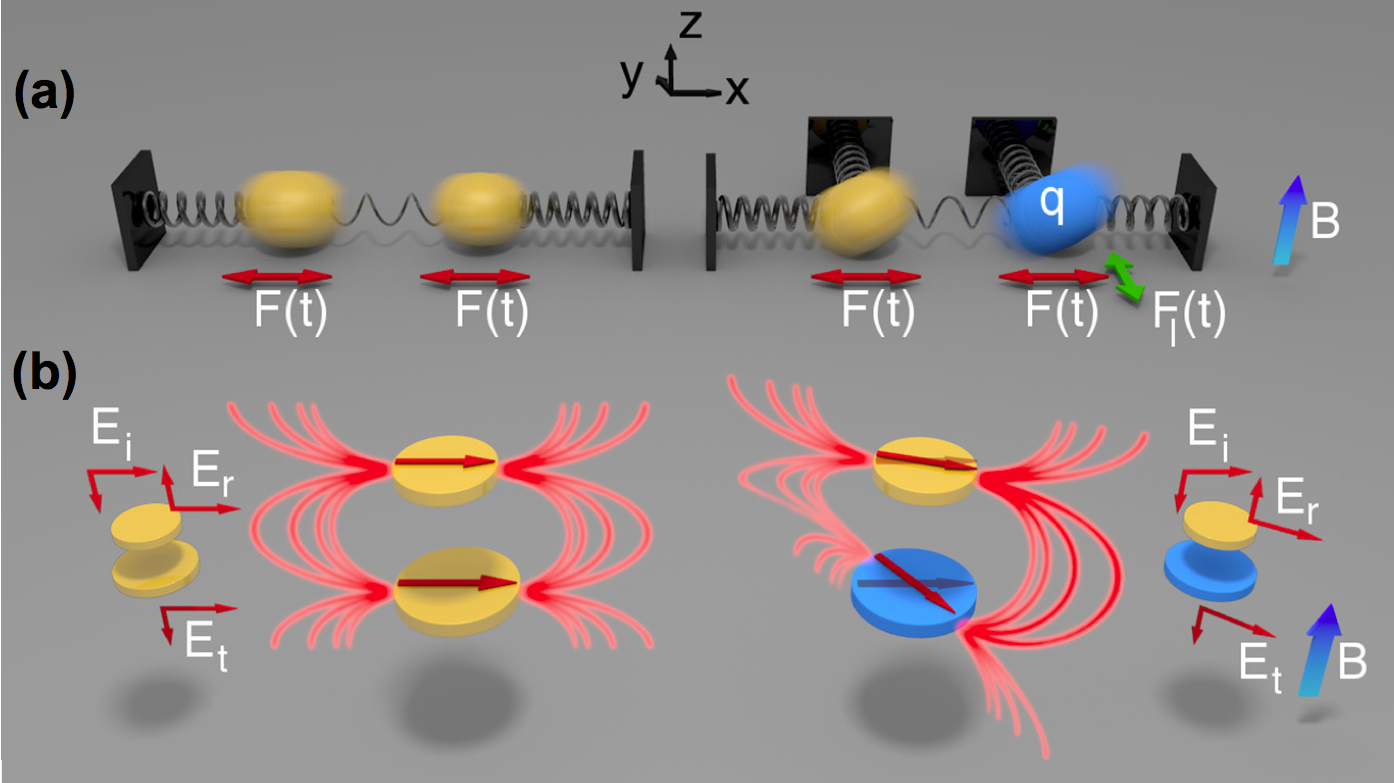
\includegraphics[width=12cm]{chapter_3/schemes/Fig_1.png} 
\par\end{centering}
\caption{ (a) Spring model representing a two coupled masses system excited by an harmonic force, $F\left(t\right)$, along $x$ axis. Left side: uncharged masses. Right side: one of the masses (blue) is charged $\left(q\right)$ and a static magnetic field $\left(\mathbf{B}\right)$ is applied along the $z-$direction, inducing a Lorentz force, $F_{1}\left(t\right)$, along the $y-$direction. The $y-$movement is transferred to the other mass through the coupling.\\
(b) Two interacting electric dipoles, representing two metallic disks, excited by an incident beam polarised along the $x$ axis. Left side: No disk has magneto-optical activity and the reflected $\left(E_{r}\right)$ and transmitted  $\left(E_{t}\right)$ light have the same polarisation direction than the incident  $\left(E_{i}\right)$ light. Right side: one of the disks (blue) has magneto-optical activity and a static magnetic field  $\left(\mathbf{B}\right)$ applied along the $z-$direction induces a rotation of its electric dipole, which is transferred to the other dipole through the interaction. The rotation modifies the polarisation direction of the reflected  $\left(E_{r}\right)$ and transmitted  $\left(E_{t}\right)$ light.\label{fig:scheme_springsdipoles}}
\end{figure}
The equations of motion are defined by:

\begin{eqnarray}
m_{1}\ddot{\mathbf{r}}_{1} & = & \mathbf{F}_{1}-k_{1}\mathbf{r}_{1}-k_{12}\left(\mathbf{r}_{1}-\mathbf{r}_{2}\right)-\mathbb{B}_{1}\dot{\mathbf{r}}_{1}, \nonumber \\
m_{2}\ddot{\mathbf{r}}_{2} & = & \mathbf{F}_{2}-k_{2}\mathbf{r}_{2}-k_{12}\left(\mathbf{r}_{2}-\mathbf{r}_{1}\right)-\mathbb{B}_{2}\dot{\mathbf{r}}_{2},
\end{eqnarray}
where the particle positions $\mathbf{r}_{i}$ are restricted to the $x-y$ plane and referred to its equilibrium
state, $k_{i}$ are spring constants, $k_{12}$ is the interaction between the particles, $m_{i}$ are their masses and, more importantly, the damping terms $\mathbb{B}_{i}$ are tensors:

\begin{eqnarray}
\mathbb{B}_{i} & = & b_{i}+F_{l}^{i}\\
 & = & \left[\begin{array}{cc}
b_{i} & 0\\
0 & b_{i}
\end{array}\right]+\left[\begin{array}{cc}
0 & -qB_{i}\\
qB_{i} & 0
\end{array}\right],
\end{eqnarray}
arising from the Lorentz force:

\begin{equation}
\mathbf{F}_{l}^{i} = qB_{i}\left[\begin{array}{cc}
0 & 1\\
-1 & 0
\end{array}\right]\left(\begin{array}{c}
\dot{r}_{x}\\
\dot{r}_{y}
\end{array}\right).
\end{equation}
It is easy to see that in the absence of a magnetic field, and considering only the friction force in a homogeneous medium, $\mathbb{B}$ can be regarded as a scalar term (diagonal with equal eigenvalues) $b$. In this case, the simple plasmonic structure without external magnetic field would be two point masses coupled in one dimension (Fig. (\ref{fig:scheme_springsdipoles})(a), left side). This system is characterised by two resonant eigenmodes, symmetric and anti-symmetric in character.\\
Is considered, without losing generality, that $m_{1} = m_{2} = m$ and that the external driving force has a harmonic temporal dependence $e^{-i\omega t}$. Thus, using the following definition:
\begin{eqnarray}
\omega_{i}^2 & = & {k_{i}}/{m} \nonumber \\
\omega_{12}^2 & = & {k_{12}}/{m}\nonumber \\
\Gamma_{i} & \equiv & \frac{\mathbb{B}_{i}}{m}\equiv \left(\begin{array}{cc}
\gamma_i & -\omega_{c,i}\\
\omega_{c,i} & \gamma_{i}
\end{array}\right),
\end{eqnarray}
the equations of motion in the frequency space become:

\begin{eqnarray}
-\mathcal{F}_{1} = \left(\omega^2 - \omega_{1}^{2} + i\omega\Gamma_{1} - \omega_{12}^{2}\right)\bold{r}_{1}+\left(\omega_{12}^2\right)\mathbf{r}_{2}\\
-\mathcal{F}_{2} = \left(\omega^2 - \omega_{2}^{2} + i\omega\Gamma_{2} - \omega_{12}^{2}\right)\bold{r}_{2}+\left(\omega_{12}^2\right)\mathbf{r}_{1},
\end{eqnarray}
where $\mathcal{F}_{i}$ is the corresponding Fourier component of the external force, $F_{i}/m\equiv\mathcal{F}_{i}$.\\
In the matrix form, this reads as:

\begin{eqnarray}
\mathbf{M}\left(\begin{array}{c}
\mathbf{r}_{1}\\
\mathbf{r}_{2}
\end{array}\right) & \equiv & \left[\begin{array}{cc}
\left(\left(\Omega_{1}^{2}-\omega_{12}^{2}\right)\mathbb{\mathbb{I}}+\omega\omega_{c,1}\sigma_{2}\right) & \omega_{12}^{2}\mathbb{I}\\
\omega_{12}^{2}\mathbb{I} & \left(\left(\Omega_{2}^{2}-\omega_{12}^{2}\right)\mathbb{\mathbb{I}}+\omega\omega_{c,2}\sigma_{2}\right)
\end{array}\right]\left(\begin{array}{c}
\mathbf{r}_{1}\\
\mathbf{r}_{2}
\end{array}\right)\nonumber \\
 & = & \left(\begin{array}{c}
-\mathcal{F}_{1}\\
-\mathcal{F}_{2}
\end{array}\right),\label{eq:chap3_mecsystem}
\end{eqnarray}
where $\mathbb{I}$ is a $2\times2$ unit matrix, $\sigma_{2}$ is the $2\times2$ Pauli matrix $\left(\sigma_{2}\equiv \left(\begin{array}{cc}
0 & -i\\
i & 0
\end{array}\right)\right)$ and $\Omega_{i}^2\equiv \omega^2 -\omega_{i}^2 + i\omega \gamma_{i}$.\\
In the problem addressed here, only one of the particles has MO activity, which is the same as to say that either $\omega_{c,1}$ or $\omega_{c,2}$ is zero (we have chosen $\omega_{c,1}$ to be zero). In order to
mimic the photonic case, the external driving force is also special, and is applied to both particles along the $x-$direction only. The solution is then:

\begin{equation}
\begin{cases}
x_1 & = - \frac{\mathcal{F}_{x}}{\cal{D}} \left[\left[\Omega_{1}^2\Omega_{2}^2-\omega_{12}^2\left(\Omega_{1}^{2}+\Omega_{2}^2\right)\right]\left(\Omega_{2}^2-2\omega_{12}^2\right)-\omega^{2}\omega_{c}^2\left(\Omega_{1}^2-\omega_{12}^2\right)\right]
\\
y_{1} & = - \frac{\mathcal{F}_{x}}{\cal{D}}\left[i\omega \omega_{c} \omega_{12}^2\left(\Omega_{1}^2-2\omega_{12}^2\right)\right] \\
x_2 & = - \frac{\mathcal{F}_{x}}{\cal{D}} \left[\left[\Omega_{1}^2\Omega_{2}^2-\omega_{12}^2\left(\Omega_{1}^{2}+\Omega_{2}^2\right)\right]\left(\Omega_{1}^2-2\omega_{12}^2\right)\right]\\
y_{2} & = - \frac{\mathcal{F}_{x}}{\cal{D}}\left[-i\omega \omega_{c} \left(\Omega_{1}^2-\omega_{12}^2\right)\left(\Omega_{1}^2-2\omega_{12}^2\right)\right],
\end{cases}\label{eq:chap3_amplitudes}
\end{equation}
where ${\cal{D}} = \omega_{12}^8 - 2\left(\Omega_{1}^2-\omega_{12}^2\right)\omega_{12}^4\left(\Omega_{2}^2-\omega_{12}^2\right) + \left[\left(\Omega_{2}^2-\omega_{12}^2\right)^2-\omega^{2}\omega_{c}^2\right]\left(\Omega_{1}^2-\omega_{12}^2\right)^2$. Details of the calculation are presented in Appendix (\ref{app:coupled_masses}).\\
In Fig. (\ref{fig:mechanicalresult}) we show the results obtained from Eq. (\ref{eq:chap3_amplitudes}), using $\mathcal{F}_x = 1 m/s^2$, $\omega_{1} = 0.9\omega_{2}$, $\gamma_{1} = 0.02\omega_2$, $\gamma_2 = 0.05\omega_{2}$, $\omega_{12} = 0.25\omega_2$, $\omega_c = 0.01\omega_{2}$.\\
Although the force is only applied in the $x-$direction and only one of the masses is charged, due to the coupling between  masses, both exhibit movement in the $y-$direction, \textit{i.e.}, from the excitation in the $x-$direction, part of the energy is converted into movement in the $y-$direction.

\begin{figure}[h!]
\begin{centering}
\par\end{centering}
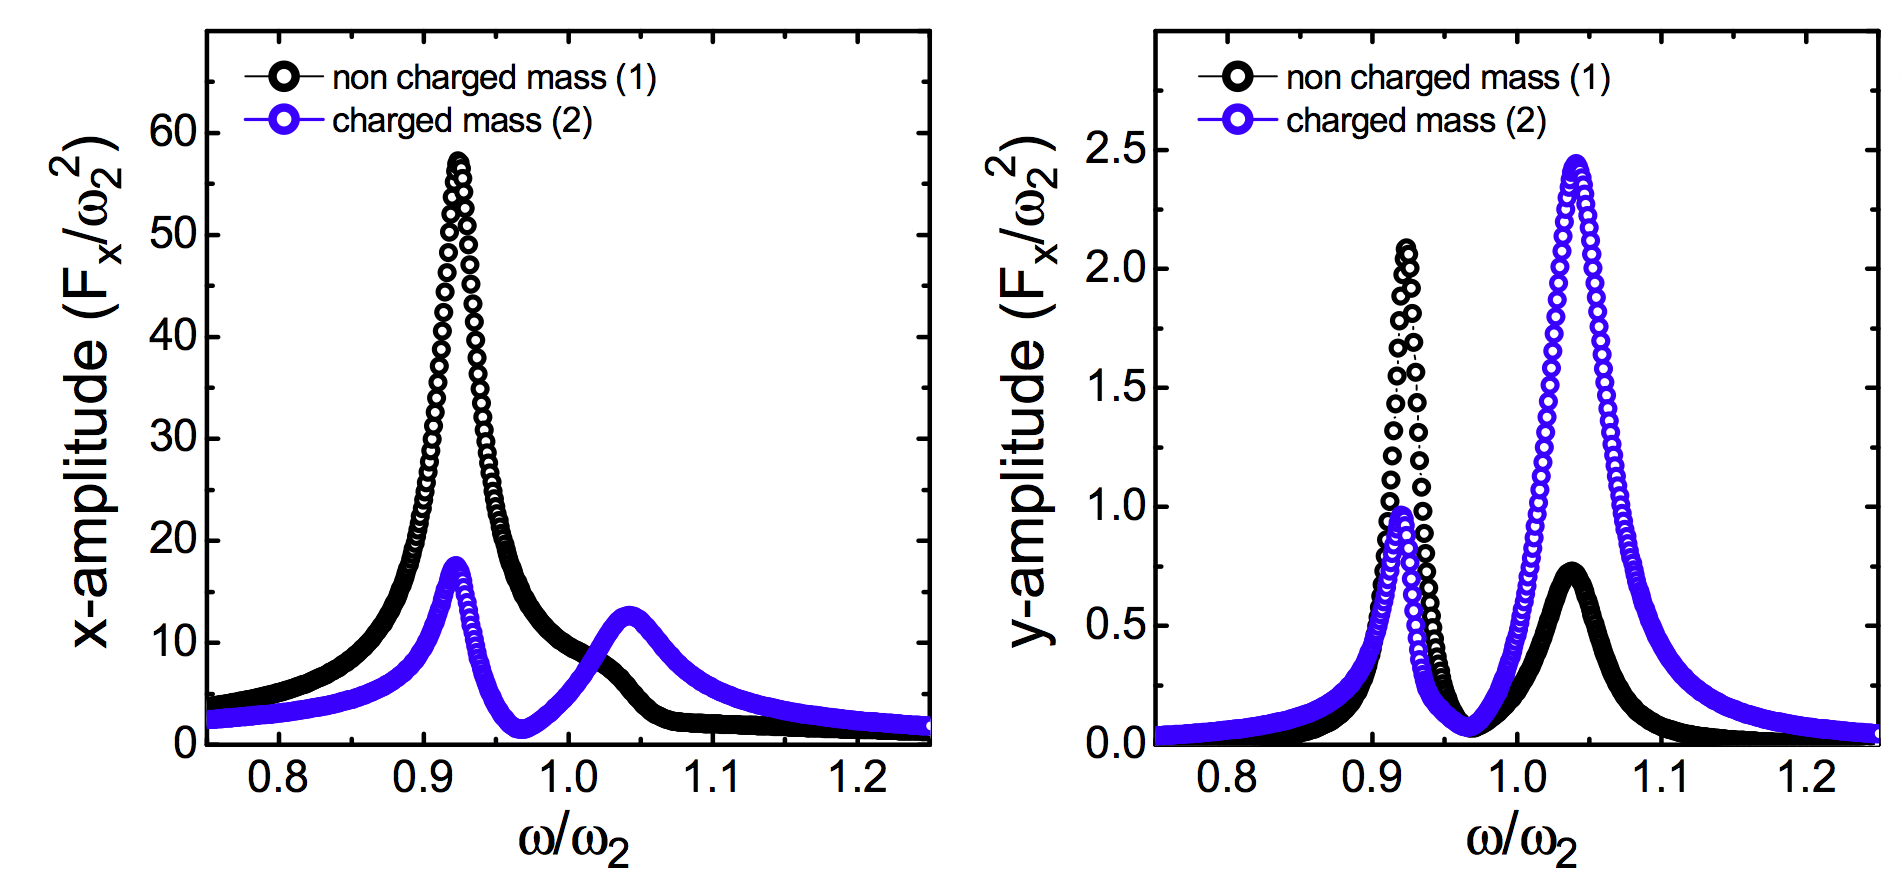
\includegraphics[width=12cm]{chapter_3/graphics/Fig_6.png} 
\caption{Oscillation amplitude as a function of the frequency of masses $1$ (uncharged) and $2$ (charged) along $x-$ (left panel) and $y-$ (right panel) direction by using a simple spring-mass model.\label{fig:mechanicalresult}}
\end{figure}

Going now to the real plasmonic case, simple structures that resemble this two coupled spring resonators system are metallic disks dimers spatially separated by a dielectric.\\
This problem can also be tackle with a simple model that substitute the disks by point dipoles, see Fig. (\ref{fig:scheme_springsdipoles})(b). These dipoles must reflect the characteristics introduced by the geometrical aspect ratio, thus the static polarisability $\boldsymbol{\alpha}_{0}$ is given by that of an oblate spheroid \cite{bohren2008absorption}:

\begin{equation}
\boldsymbol{\alpha}_{0} = \nu \left[\boldsymbol{\epsilon}-\mathbb{I}\right]\left[\mathbb{I}+\mathbb{L}\left(\boldsymbol{\epsilon - \mathbb{I}}\right)\right]^{-1}, \label{eq:chap3_polarizability}
\end{equation}
 and we take into account that the dielectric tensor is not diagonal, and consider radiative corrections \cite{albaladejo2010radiative}:

\begin{equation}
\boldsymbol{\alpha} = \boldsymbol{\alpha}_{0}\left[\mathbb{I}-i\frac{k^3}{6\pi}\boldsymbol{\alpha}_{0}\right]^{-1},\label{eq:chap3_radiative_correction}
\end{equation}
where $\nu$ is the volume of the spheroid, $\mathbb{L}$ is a diagonal matrix that takes care of the geometrical aspect (see Appendix (\ref{App:pol_oblate_sphe})), and the environment is vacuum.\\
The interaction between the two dipoles is given by the Green tensor:

\begin{equation}
\mathbf{G}\left(\mathbf{r},\mathbf{r}'\right) = \frac{e^{ikR}}{4\pi R}\left[\left(1+\frac{ikR-1}{k^2R^2}\right)\mathbb{I}+\frac{3-3ikR-k^2R^2}{k^2R^2}\frac{\mathbf{R} \otimes\mathbf{R}}{R^2}\right],\label{chap3_Green_tensor}
\end{equation}
where $\mathbf{R} = \mathbf{r} - \mathbf{r}'$ and $R$ is the absolute value. \\
With these definitions the incident electric field on a particle $i$ originated from an ensemble of ${\cal{N}}$ particles is given by:

\begin{equation}
\mathbf{E}\left(\mathbf{r}_i\right) = \mathbf{E}_{0}\left(\mathbf{r}_i\right) + \frac{k^2}{\epsilon_{0}}\sum_{i \neq j}^{\cal{N}}\mathbf{G}\left(\mathbf{r}_i,\mathbf{r}_j\right) \mathbf{p}_j,
\end{equation}
where $\mathbf{p}_j = \epsilon_{0}\boldsymbol{\alpha}_i\mathbf{E}\left(\mathbf{r}_j\right)$ is the polarisation of particle $j$. Since the incident wave $\mathbf{E}_{0}\left(\bold{r}\right)=E_{0}e^{-ikz}\bold{u}_x$ is polarised along the $x-$axis and its wavevector is parallel to the $z-$axis (short axis of the particles), the polarisation of the particles lies in the $x-y$ plane:

\begin{equation}
\boldsymbol{\alpha}\left(\omega\right)=\left[\begin{array}{ccc}
\alpha_{i,xx} & \alpha_{i,xy} & 0\\
-\alpha_{i,xy} & \alpha_{i,xx}& 0\\
0 & 0 & \alpha_{i,zz}
\end{array}\right],\label{eq:chap3_polarizabilitytensor}
\end{equation}
and the Green tensor that describes the interaction of the two particles (placed along $z-$axis) is diagonal and its given by:

\begin{equation}
\mathbf{G}\left(\mathbf{r}_1,\mathbf{r}_2\right) = \mathbf{G}\left(\mathbf{r}_2,\mathbf{r}_1\right) = \mathcal{G}\mathbb{I}=\frac{e^{ikd}}{4\pi d}\frac{\left(kd\right)^2+ikd-1}{\left(kd\right)^2}\mathbb{I},\label{eq:chap3_greenf}
\end{equation}
being $d$ the distance between the particles. One has to take into account that with the geometry described above the $z-$direction plays no role and can be excluded. The equations to deal with are:

\begin{equation}
\begin{cases}
\frac{\boldsymbol{\alpha}_{1}^{-1}}{\epsilon_0} \bold{p}_1 & = \bold{E}_0\left(\bold{r}_1\right) + \frac{k^2}{\epsilon_0}\mathcal{G}\bold{p}_2 =  \bold{E}_{0,1x}+\frac{k^2}{\epsilon_0}\mathcal{G}\bold{p}_2\\
\frac{\boldsymbol{\alpha}_{2}^{-1}}{\epsilon_0} \bold{p}_2 & = \bold{E}_0\left(\bold{r}_2\right) + \frac{k^2}{\epsilon_0}\mathcal{G}\bold{p}_1 =  \bold{E}_{0,1x}e^{i\delta}+\frac{k^2}{\epsilon_0}\mathcal{G}\bold{p}_1,
\end{cases}\label{eq:app_syspol}
\end{equation}
where $\boldsymbol{\alpha}_i$ is the $2\times2$ $x-y$ part of the tensor described in Eq. (\ref{eq:chap3_polarizabilitytensor}), and $\delta = -kd$ is the phase difference on the incoming wave due to the separation distance $d$ (normally $\delta \ll 1$).\\
With that is easy to see that we end with the following set of equations:

\begin{equation}
\mathbf{M}\left[\begin{array}{c}
\mathbf{p}_{1}\\
\mathbf{p}_{2}
\end{array}\right]\equiv\left[\begin{array}{cc}
\frac{\boldsymbol{\alpha}_{1}^{-1}}{\epsilon_{0}} & -\frac{k^2}{\epsilon_{0}}\mathcal{G}\mathbb{I}\\
-\frac{k^2}{\epsilon_{0}}\mathcal{G}\mathbb{I} & \frac{\boldsymbol{\alpha}_{2}^{-1}}{\epsilon_0}
\end{array}\right]\left(\begin{array}{c}
\mathbf{p}_{1}\\
\mathbf{p}_{2}
\end{array}\right)=\left(\begin{array}{c}
\mathbf{E}_{0,1}\\
\mathbf{E}_{0,1}e^{i\delta}
\end{array}\right),
\end{equation}
which as the same structure of Eq. (\ref{eq:chap3_mecsystem}) for only one MO dipole (dipole 2).
The solution is now straightforward:

\begin{equation}
\begin{cases}
p_{1x} & = \epsilon_{0}\frac{E_{0,1x}}{\cal{D}} \alpha_1 \left[1+k^2\mathcal{G}\alpha_{2xx}\left(e^{i\delta}-k^2\mathcal{G}\alpha_1\right)-k^6\mathcal{G}^3\alpha_1\left(\alpha_{2xx}^2+\alpha_{2xy}^2\right)e^{i\delta}\right]
\\
p_{1y} & = -\epsilon_{0}\frac{E_{0,1x}}{\cal{D}} k^2\mathcal{G}\alpha_1 \alpha_{2xy}\left[e^{i\delta}+k^2\mathcal{G}\alpha_{1}\right] \\
p_{2x} & = \epsilon_{0}\frac{E_{0,1x}}{\cal{D}} \left[\alpha_{2xx}-k^4\mathcal{G}^2\alpha_1 \left(\alpha_{2xx}^2+\alpha_{2xy}^2 \right)\right]\left[e^{i\delta}+k^2\mathcal{G}\alpha_1\right]\\
p_{2y} & = -\epsilon_{0}\frac{E_{0,1x}}{\cal{D}} \alpha_{2xy}\left[e^{i\delta}+k^2\mathcal{G}\alpha_1\right],
\end{cases}\label{eq:chap3_polarizations_solution}
\end{equation}
where $\mathcal{D} = 1 - 2k^4\mathcal{G}^2\alpha_{1}\alpha_{2xx}+k^8\mathcal{G}^4\alpha_1^2\left(\alpha_{2xx}^2+ \alpha_{2xy}^2\right)$. The detailed calculations are done in Appendix (\ref{App:coupled_oscillators}).

\begin{figure}[h!]
\begin{centering}
\par\end{centering}
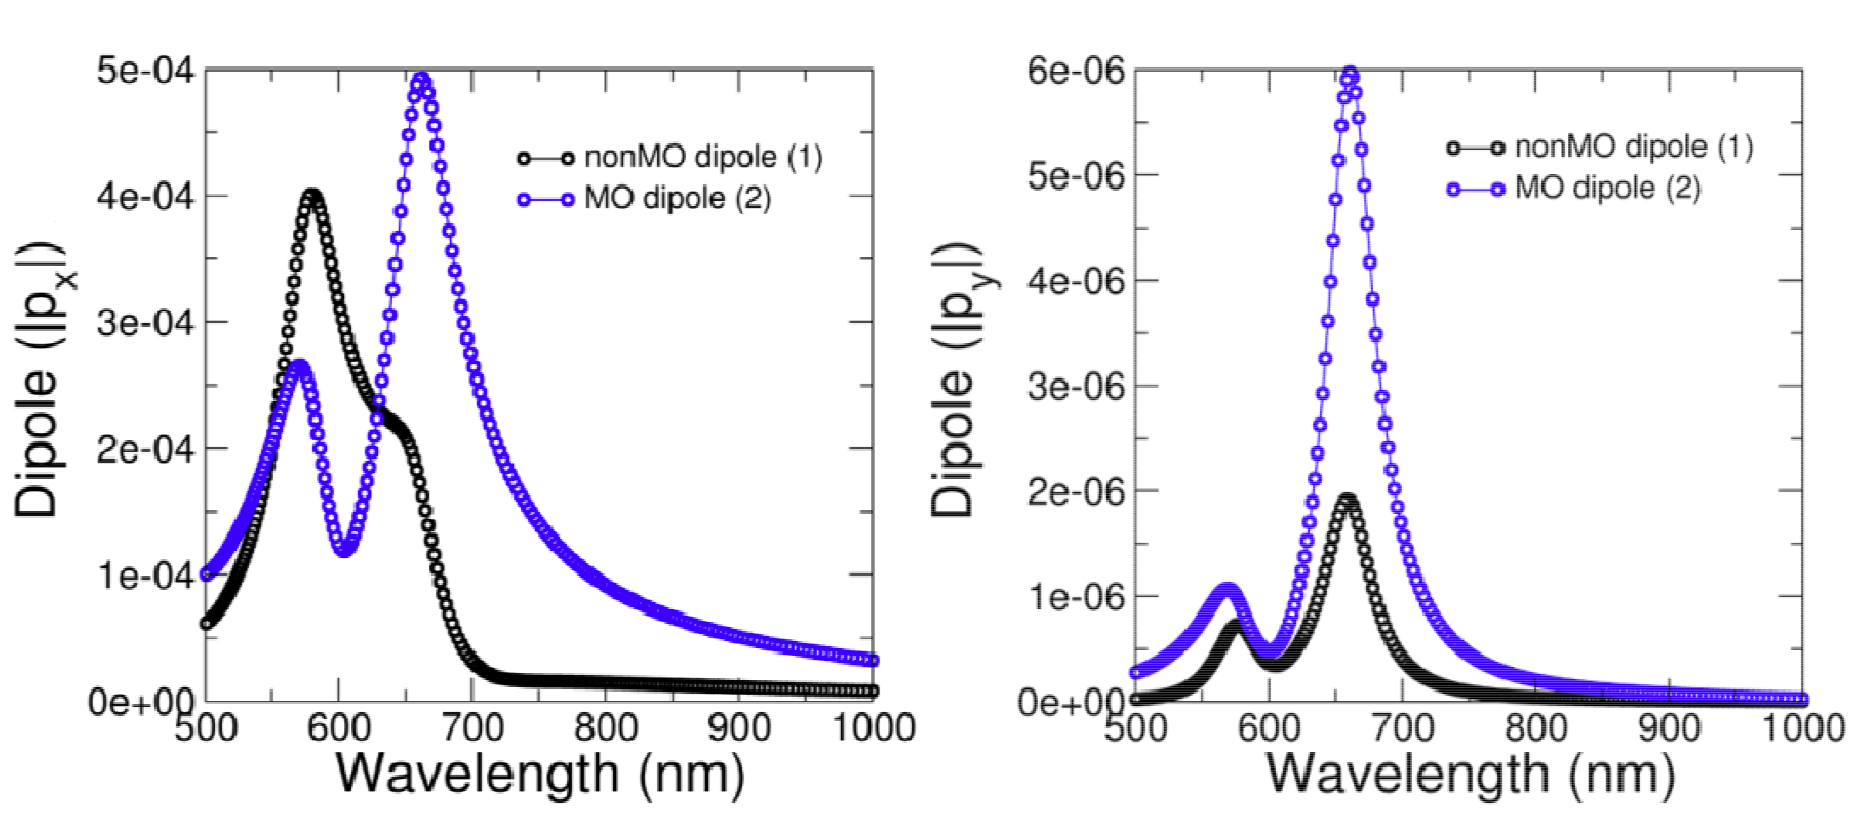
\includegraphics[width=12cm]{chapter_3/graphics/Fig_7.png} 
\caption{Wavelength dependence of the normalized dipole magnitudes along the $x-$ (left panel) and $y-$ (right panel) directions obtained using a point dipole model.\label{fig:dip_result}}
\end{figure}

In Fig. (\ref{fig:dip_result}) is shown the results obtained from Eq. (\ref{eq:chap3_polarizations_solution}) for intermediate interaction. Like in the mechanical case, the electric field is applied in the $x-$direction and only one of the dipoles is MO. Due to the electromagnetic coupling, both exhibit polarisation in the $y-$component.

The interaction between the electric dipoles gives rise to bright and dark modes (or more precisely, superradiant and subradiant modes), whose spectral position and character can be tuned by the thickness of the separating dielectric \cite{dmitriev2007gold, pakizeh2008structural, ekinci2008electric}. In the simple model presented here and schematically shown in Fig. (\ref{fig:scheme_springsdipoles})(b), left side, the bright mode corresponds to the configuration in which the electric dipoles are oriented parallel to each other (symmetric mode), while in the dark case the dipoles are oriented antiparallel (anti-symmetric mode). In both cases the electric dipoles are along x axis (parallel to the electric field of the incoming light). If one of the disks has ferromagnetic character, the application of a magnetic field along $z-$direction will induce a rotation of its associated dipole about this axis (Fig. (\ref{fig:scheme_springsdipoles})(b), right side). Extrapolating what it is obtained in the spring-mass case, the transverse oscillation induced in the uncharged mass will manifest here as an induced rotation of the dipole of the non-ferromagnetic metallic disk. The combined rotation of both dipoles will cause polarisation conversion effects. In this sense, magneto-optics is the appropriate tool to explore this new degree of freedom, since it provides a direct measurement of the magnetic field induced polarisation conversion.

\section{Optical and magneto-optical response of nanoresonators \label{sec:chap3_nanoresonators}} 

In order to confirm the previous results, we analyse structures that consist of a pure $\textnormal{Au}$ nanodisk separated by a $\textnormal{SiO}_{2}$ spacer from a $2nm\textnormal{Co}/4nm\textnormal{Au}$ multilayer nanodisk. The presence of $\textnormal{Au}$ in the bottom magnetoplasmonic disk reduces its optical losses as compared to a pure ferromagnetic metal disk \cite{armelles2013magnetoplasmonics}. The disks were fabricated using hole-mask colloidal lithography and evaporation (electron beam evaporation for $\textnormal{Co}$ and $\textnormal{SiO}_{2}$ layers and thermal evaporation for $\textnormal{Au}$ layers) \cite{banthi2012high, fredriksson2007hole}. In Fig. (\ref{fig:SEM_disk})(a) we show a sketch of the internal structure of each disk with the characteristic individual layer thickness. The $\textnormal{Au}/\textnormal{Co}$ multilayer disk exhibits perpendicular magnetic anisotropy, reducing the magnetic field required to achieve saturation in polar configuration, Fig. (\ref{fig:SEM_disk})(b). Fig. (\ref{fig:SEM_disk})(c) presents a cross section Scanning Electron Microscopy image of the same structure showing the truncated nanocone shape of the obtained nanoresonators, whose typical lower and upper disk diameters are $110-120nm$ and $70-90nm$ respectively. In this cross section image, both the metallic and dielectric components of the nanodisks are clearly distinguishable. Additionally, in Fig. (\ref{fig:SEM_disk})(d) a top view image of a representative structure, showing the homogeneous distribution of the disks over large areas, is presented.

\begin{figure}[h!]
\begin{centering}
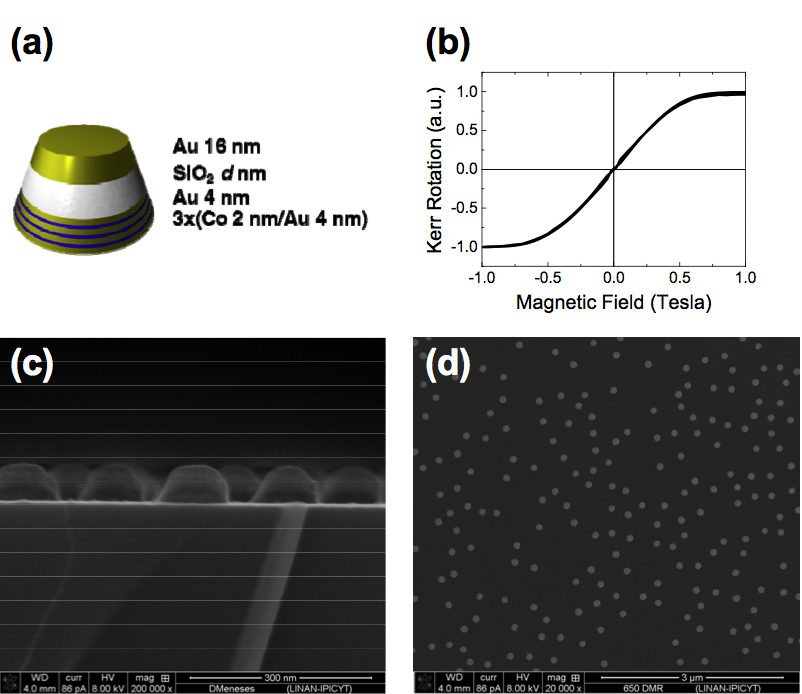
\includegraphics[width=10cm]{chapter_3/graphics/Fig_2.png} 
\par\end{centering}
\caption{(a) Schematic drawing of the nanoresonators composed of a purely plasmonic $\textnormal{Au}$ disk and a magnetoplasmonic $\textnormal{Au}/\textnormal{Co}$ superlattice disk separated by a dielectric spacer. (b) Polar Kerr loop of a characteristic sample. The presence of multiple $\textnormal{Co}/\textnormal{Au}$ interfaces reduces the value of the magnetic field needed to saturate the nanodisks in the direction perpendicular to the sample plane. (c), (d) Cross section and planar view SEM pictures, respectively, of a representative sample. The images show the homogeneous and random distribution of nanoresonators and their truncated conical shape and internal structure.\label{fig:SEM_disk}}
\end{figure}

In the left column of Fig. (\ref{fig:exp_extintion}) is shown the measured extinction spectra as a function of the $\textnormal{SiO}_{2}$ spacer thickness. As it can be seen, the spectral dependence of the extinction strongly varies as a function of the dielectric thickness, {\it{i.e.}}, with the inter-disk interaction. For the extreme case of thick $\textnormal{SiO}_{2}$ $\left(50 nm\right)$, both metallic disks interact weakly, and as a consequence two peaks corresponding to the individual disk resonances are observed. Thus, the high-energy peak can be identified with the resonance of the top metallic disk (smaller diameter) and the low energy one with that of the bottom one (larger diameter). As the $\textnormal{SiO}_{2}$ spacer gets thinner, the position and relative intensity of both resonances changes. In this situation, both modes become hybridised \cite{prodan2003hybridization, dmitriev2007gold} and we can no longer talk of individual modes but of complex modes of symmetric and anti-symmetric character. The symmetric mode, occurring at higher energies, strongly couples to the incident light and as a consequence has a larger extinction (bright or superradiant mode). On the other hand, the anti-symmetric mode, occurring at lower energies, couples weakly to the light, resulting in a lower extinction peak (dark or subradiant mode). Qualitatively, the symmetric mode is clearly observed for all the structures, while the anti-symmetric one gradually decreases in intensity, shifting to lower energies as the spacer becomes thinner, becoming practically unobservable for ${2}$ thickness below $15 nm$.\\

\begin{figure}[h!]
\begin{centering}
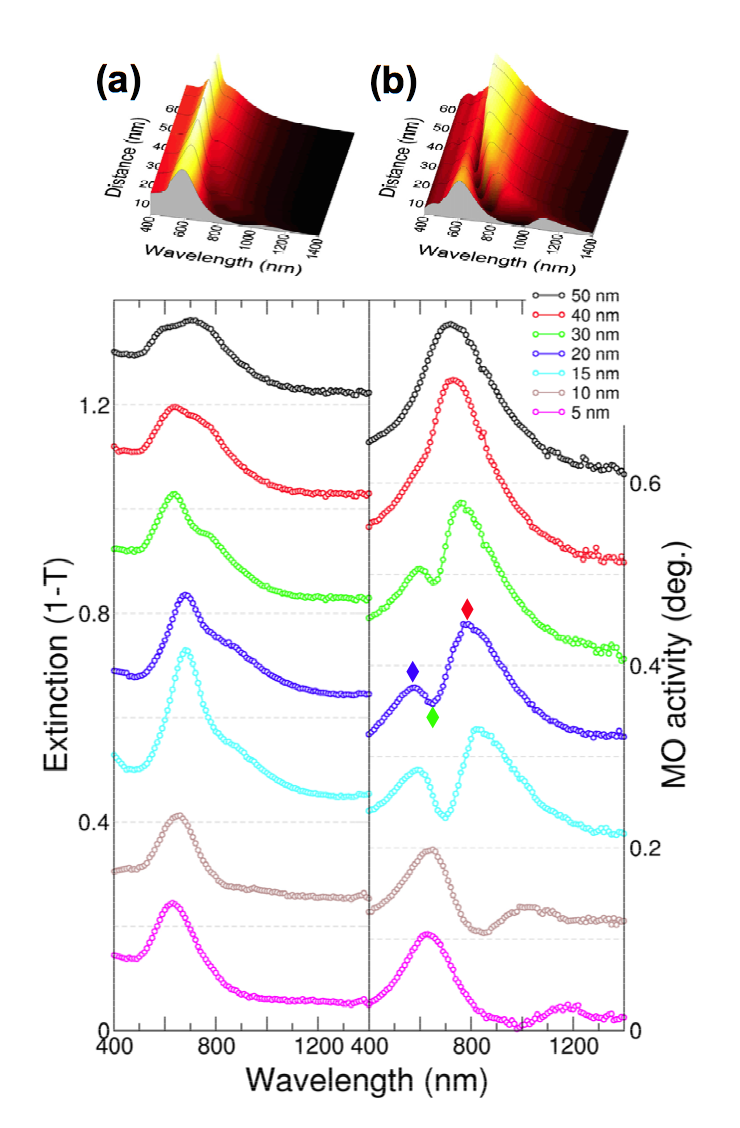
\includegraphics[width=8cm]{chapter_3/graphics/Fig_3.png} 
\par\end{centering}
\caption{(a) Extinction and (b) MO activity spectra of the nanoresonators as a function of $\textnormal{SiO}_{2}$ thickness. The different dashed horizontal lines indicate the zero value for each spectrum above the line. The 3D graphs on top of each panel show the results obtained from theoretical calculations of the same structures. The blue, green and red diamonds appearing in the experimental MO response for $20 nm$ $\textnormal{SiO}_{2}$ correspond to the spectral positions where the $E_{z}$ field distributions are calculated (see Fig. (\ref{fig:colormaps})).\label{fig:exp_extintion}}
\end{figure}

The right hand column of Fig. (\ref{fig:exp_extintion}) shows the spectral dependence of the MO activity of the same nanostructures, corresponding to the modulus of the complex Polar Kerr rotation, $\Phi$ (where $\Phi = \theta + i\phi$, being $\theta$ and $\phi$ the Polar Kerr rotation and ellipticity respectively, as presented in Sec. (\ref{sec:chap2_dielectric_tensor})), measured at normal incidence and magnetic saturation. Unlike simple fully metallic $\textnormal{Au}/\textnormal{Co}/\textnormal{Au}$ nanodisks where MO activity and extinction spectra are directly related \cite{gonzalez2008plasmonic}, the spectra of our nanodisk dimers exhibit a strong dependence on the spacer thickness but with distinctive differences with respect to the extinction spectra. For example, for thick spacer layers only one peak is observed, contrary to the double peaked spectral dependence of the extinction. This peak corresponds to the MO activity of the bottom disk, which actually is the only one with a ferromagnetic constituent. The upper disk, made up of pure $\textnormal{Au}$, does not contribute to the MO activity of the structure. However, as the $\textnormal{SiO}_{2}$ becomes thinner and the electromagnetic (EM) interaction between both metallic disks increases, a new peak appears at higher energy, whose position hardly depends on the spacer thickness. On the other hand, the low energy MO peak gradually red shifts and loses intensity as the spacer thickness is reduced. Additionally, and contrary to what was observed in the extinction measurements, this low-energy peak is observed all the way down to the thinnest dielectric spacer in the MO case. Special mention deserves the specific MO peak shapes for intermediate spacer thickness (between $15$ and $30 nm$), where the two MO peaks are energetically close. In this regime the MO spectra are clearly not the result of the convolution of two peaks that would originate from independent modes, but rather exhibit a typical Fano resonance shape, which on the other hand is absent in the extinction spectra.\\
To further link the experimental results with the dipole model, we have performed rigorous simulations for both the extinction and MO response, based on scattering matrix techniques \cite{garcia2005light, caballero2012generalized} and FDTD \cite{lumericalcite} as well as FEM \cite{comsolcite} codes. The three methods provide equivalent results. The evolution of the spectra as a function of the $\textnormal{SiO}_{2}$ thickness is depicted as 3D graphs on top of the corresponding columns in Fig. (\ref{fig:exp_extintion}), exhibiting a very good agreement with the experimental results, both regarding the intensity, spectral shape, and peak position evolution. In addition to the mentioned extinction and MO activity, the performed simulations allow also obtaining the EM field distribution in regions around the nanodisks. As an example we present in Fig. (\ref{fig:colormaps}) the near field distribution of the $z-$component of the electric field, for the sample with $20nm$ $\textnormal{SiO}_{2}$ spacer, in two planes at $10 nm$ above the top and below the bottom disks respectively, both in the absence of an external magnetic field and as the difference for magnetic saturations along opposite directions. These distributions have been calculated for the three wavelengths corresponding to the two maxima and the minimum of the MO activity (labelled with red, green and blue diamonds in Fig. (\ref{fig:exp_extintion})).\\
The $E_{z}$ component without external magnetic field (extinction measurements situation) is presented in the left panel of Fig. (\ref{fig:colormaps}). There, for the low energy position (red framed) the EM distribution for each metallic disk resembles that of a point dipole oscillating along the $x-$direction, with similar $E_{z}$ intensity for both upper and lower disk, and with the individual dipoles (represented by the black arrows in Fig. (\ref{fig:colormaps})) oriented antiparallel (note that the $E_{z}$ field of a dipole changes sign when it is seen from above or from below). This situation therefore corresponds to the aforementioned anti-symmetric configuration. On the other hand, for the high energy position (blue framed) the EM distribution for each metallic disk corresponds also to a dipole-like distribution along the $x-$direction but now the individual dipoles corresponding to the disks are oriented parallel to each other (symmetric mode). As it can be seen, the intensity of the $E_z$ component for both disks is, again, similar, but larger than that for the low energy case. This is consistent with the higher extinction value obtained for the symmetric mode respect to the anti-symmetric one. Finally, at the intermediate energy (green framed), the distribution is still dipolar-like and would correspond to a symmetric-like mode, but the intensity distribution is not equally distributed, with a larger value of the $E_z$ component in the upper disk than for the lower one.

\begin{figure}[h!]
\begin{centering}
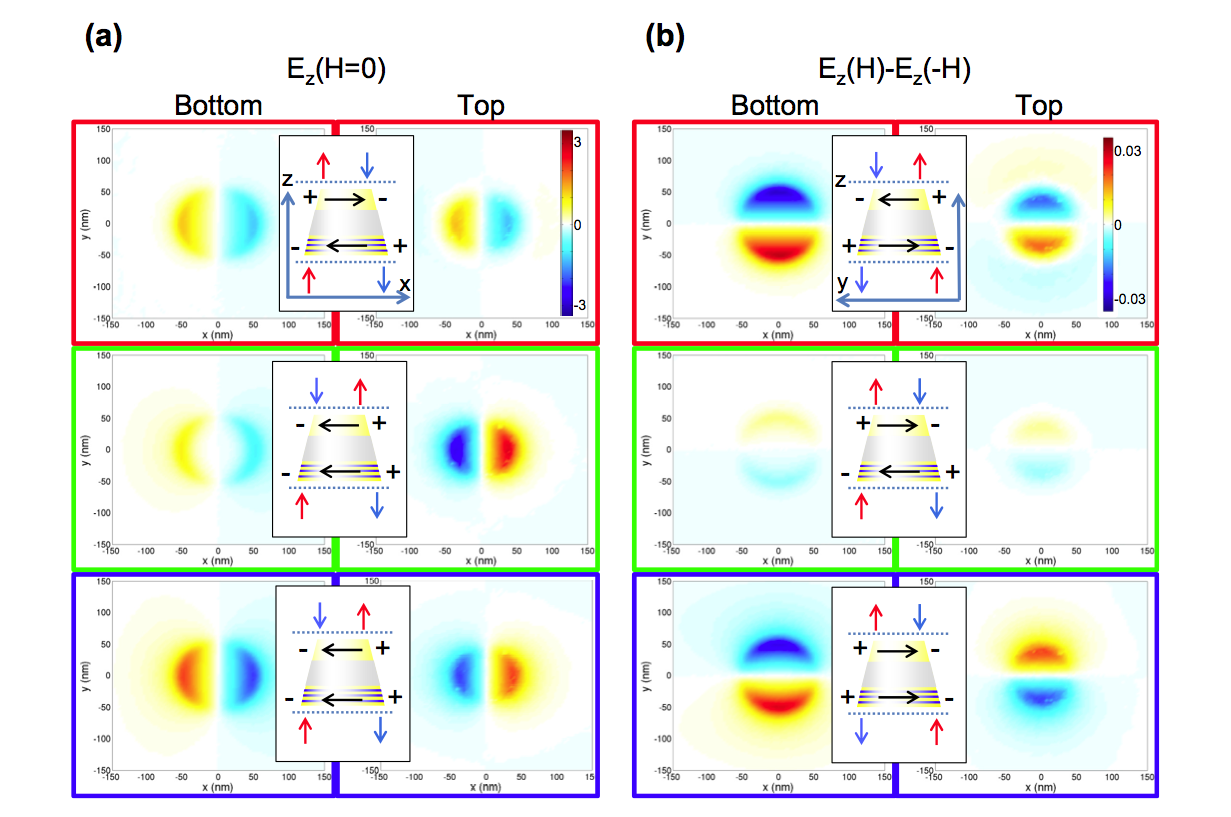
\includegraphics[width=12cm]{chapter_3/graphics/Fig_4.png} 
\par\end{centering}
\caption{(a) Calculated near field intensity of the $E_z$ component for a nanoresonator with $20$ nm $\textnormal{SiO}_2$ spacer in two planes above the top disk and below the bottom one, with the incident field polarised along the $x$ direction and in the absence of an external magnetic field. This distribution reflects the excitation of two dipoles along the $x$ direction. The insets indicate the corresponding charges and dipole orientations (indicated by the black arrows) according to the $E_z$ distribution for the different cases. The red (blue) arrows in the insets represent the positive (negative) values of the $E_z$ field component. (b) Difference of the $E_z$ components for magnetic saturation along opposite directions in the same planes and for the same structure. This difference accounts for the effect of the applied magnetic field: The appearance of a dipole along the $y-$direction for both the magnetoplasmonic (intrinsic dipole) and the plasmonic (induced dipole) disks. In both cases, the components for three different wavelengths labelled as diamonds in Fig. (\ref{fig:exp_extintion}) are shown.\label{fig:colormaps}}
\end{figure}

Next, in the right panel of Fig. (\ref{fig:colormaps}) we show the difference between $E_z$ components at magnetic saturation along opposite directions, $E_{z}(H)-E_{z}(-H)$ (MO measurements situation) which reflects the magnetic field effect on the field distributions of the system eliminating the purely optical contribution. For the three energies, a dipolar-like distribution is still observed, but the resulting balance between magnetic saturation along opposite directions is an $E_{z}$ component corresponding to a point dipole oscillating along the $y-$direction. In other words, the effect of the magnetic field is to induce a "dipole" along the $y-$direction that is two orders of magnitude smaller in intensity than the dipole generated along the $x-$direction.\\
On the other hand, regarding the symmetry character of the resulting modes, it is maintained for high and low energies with respect to the case of no magnetic field applied: anti-symmetric and symmetric for low and high energy respectively. Regarding the intensities of the $E_{z}$ fields, it is similar for top and bottom disks and for both energies. The induction by the magnetic field of a dipole along $y-$direction is pretty intuitive for the bottom disk, since it is simply due to the presence of ferromagnetic material in it. What is in principle not as intuitive is the presence of the same component in the upper disk, since it has no ferromagnetic nature. This $y-$component in the upper disk is induced by the "dipole" of the bottom disk, reaching a sizeable magnitude. More interestingly, the situation for the intermediate energy, corresponding to the minimum of the MO activity, is quite different. In this case both lower and upper disks, regardless the presence of a ferromagnetic component in its interior, exhibit almost zero MO-induced "dipoles".

\section{Discussion\label{sec:chap3_discussion}}

From the observation of the resulting $E_{z}$ components, one can conclude that the application of a magnetic field has three main effects: first, it generates a "dipolar" component along the $y-$direction not present without magnetic field; second, mediated by the interaction between the disks, the bottom disk, which has a ferromagnetic component, induces a "dipole" along the $y-$direction in the upper disk, in other words it generates a MO activity in a disk which has no ferromagnetic nature; third, there is a spectral region were both "dipoles" vanish almost completely, and therefore, the MO activity is strongly reduced.\\
To understand the physical origin of this phenomenology, let us consider the field distributions obtained for the intermediate energy region shown in the left panel of Fig. (\ref{fig:colormaps}). In that region, the intensity of the field at the bottom disk clearly decreases with respect to the other two energies considered. This suggests that the electric field induced by the upper disk destructively interferes with the incoming electric field. This can be understood from the simple model based on two interacting point dipoles. From the solution of the dipole model, Eq. (\ref{eq:chap3_polarizations_solution}), is identified a common term $\left[e^{i\delta}+k^2{\cal{G}}\alpha_{1}\right]$ for both $x-$ and $y-$components of the dipole with MO activity ($\bold{p}_2$) and the $y-$component of the dipole with no MO activity ($\bold{p}_1$). This term is related to the total electric field along the $x-$direction at the MO active dipole, and results from the addition of the incident field and the field generated at this point by the dipole with no MO activity. If this term vanishes the three components die out, and therefore the MO activity is suppressed. On the other hand, as the $x-$component of the dipole with no MO activity does not depend on this term, it is not cancelled being the only one that contributes to the optical response of the whole system. From the point of view of the mechanical model this situation corresponds to the transition region between the in-phase and out-of-phase oscillations of the masses: the charged mass decreases its oscillation and therefore the Lorentz force, proportional to the velocity, is strongly attenuated. As a consequence, the movement of this mass along the $y-$direction and the induced movement of the uncharged mass are also reduced.\\
This phenomenon can be viewed as the MO counterpart of the electromagnetic induced transparency. For a specific spectral region, the EM interaction between the two disks gives rise to a situation where the total EM field at the MO active element is minimised, therefore strongly reducing the MO activity of the whole system, (see Eq. (\ref{eq:chap3_polarizations_solution})). This is observed in Fig. (\ref{fig:chap3_MO_activity})(a), where we present the experimental MO activities for two different situations corresponding to very weak interaction (the $50 nm$ $\textnormal{SiO}_2$ structure) and a situation where the two disks clearly interact (the $20 nm$ $\textnormal{SiO}_2$ structure). For the very weak interacting system only a broad peak is observed, corresponding to the MO activity of the magnetoplasmonic disk. However, for the system where the two metallic disks interact, a narrow dip with a clear Fano-like shape is obtained. The difference between both spectra is also shown (inset), presenting a narrow peak.\\
\begin{figure}[h!]
\begin{centering}
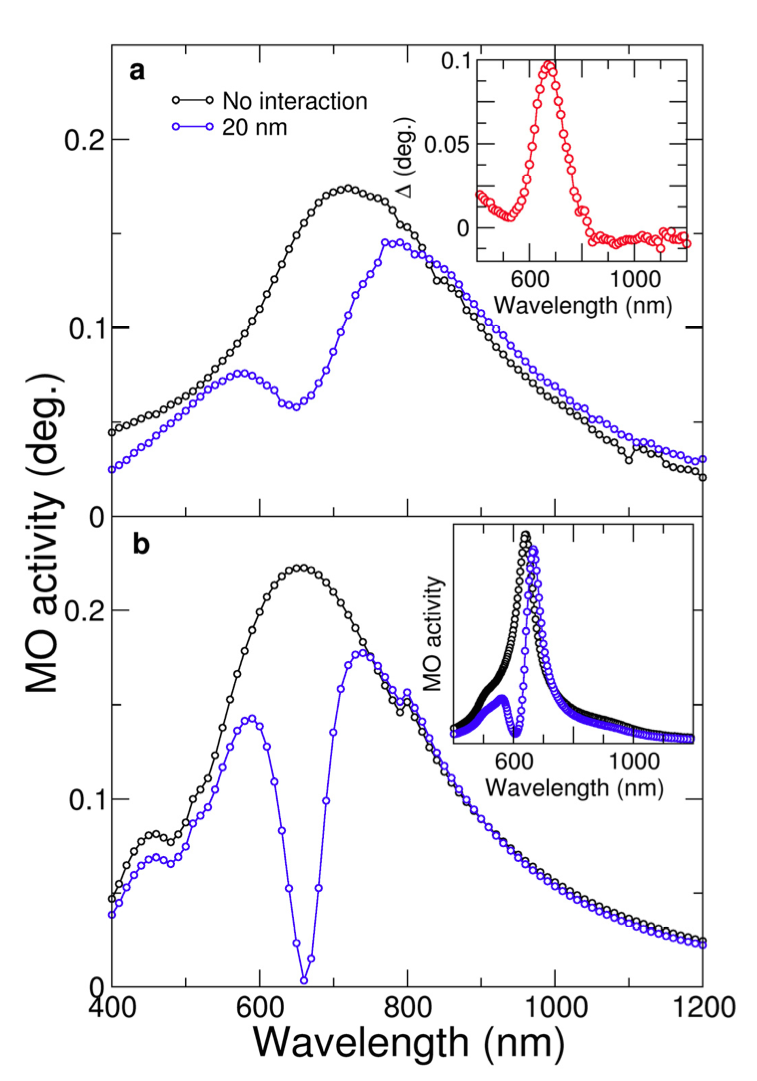
\includegraphics[width=8cm]{chapter_3/graphics/Fig_5.png} 
\par\end{centering}
\caption{Fano resonance in the magneto-optical activity. (a) Experimental spectra of the MO activity for the structures with $20 nm$ and $50 nm$ $\textnormal{SiO}_2$ spacer, corresponding to interacting and non interacting situations, respectively. For the interacting situation a clear Fano resonance shape is observed. The inset shows the difference between the two spectra, resulting in a narrow peak.\\
(b) Theoretical MO activity spectra obtained for a structure with $20nm$ $\textnormal{SiO}_2$ spacer and for the same structure but without the upper metallic disk. The inset shows the MO spectra obtained using the simple point dipole model.\label{fig:chap3_MO_activity}}
\end{figure}
Fano resonances are observed whenever a broad and a narrow state interfere destructively, giving rise to a sharp spectral feature. In our specific case, the broad state corresponds to the EM field at the MO disk in the absence of interaction, whereas the narrow one is due to the electromagnetic field induced by the non-MO disk at the MO disk. Due to its intrinsic interaction origin, this Fano shape strongly depends on the $\textnormal{SiO}_2$ spacer thickness. As it can be seen in Fig. (\ref{fig:exp_extintion}), for thick enough $\textnormal{SiO}_2$ spacers, the MO activity is simply that of an individual disk (the bottom disk) and, as the spacer thickness is gradually reduced, the interaction between the disks becomes more relevant and, especially for intermediate spacer thickness, the Fano-like shape is clear. This interaction dependence appears explicitly in the common term of Eq. (\ref{eq:chap3_polarizations_solution}) as the field propagator ${\cal{G}}$ depends on the distance between the two dipoles. In Fig. (\ref{fig:chap3_MO_activity})(b) we also present the calculated MO activity using a transfer matrix formalism or a simple dipolar model (inset) for two cases corresponding to a structure without the upper disk (no interaction) and a structure with both disks separated by a $20 nm$ thick $\textnormal{SiO}_2$ layer. As it can be observed the calculated results follow the same trends as the experimental ones.

\section{Conclusion \label{sec:chap3_conclusions}}
In conclusion, MO activity in non-MO elements can be induced via electromagnetic interaction with MO active elements. This effect has been shown in magnetoplasmonic resonators consisting of a $\textnormal{Au}$ plasmonic disk separated by a $\textnormal{SiO}_{2}$ layer from a MO active magnetoplasmonic $\left(\textnormal{Au}/\textnormal{Co}\right)$ disk. When a magnetic field is applied perpendicular to the disks, it produces an electric dipole along the perpendicular direction of the electric field of the incoming light in the MO active disk. This electric dipole induces a MO activity in the non- magnetic $\textnormal{Au}$ disk. Additionally, we have shown the existence of an electromagnetically induced magneto-optical transparency in these systems. This is due to the interference at the MO disk between the incidence electromagnetic field and that generated by the non-MO one, leading to a Fano-like spectral dependence of the MO activity and to a strong reduction of the MO activity. This may find applications in sensing architectures based on MO-Fano resonances. Optical Fano resonances have already demonstrated their potential applicability \cite{yanik2011seeing, wu2012fano, offermans2011universal}. Additionally, plasmon excitation enhancement of the MO activity has also shown improvement of the performance of standard plasmonic sensors \cite{sepulveda2006highly, bonanni2011designer}. Combining both effects may allow the generation of novel sensing platforms based on MO-Fano resonances. Since the observed phenomenon is driven by the resonance of the upper disk, modifications of the dielectric environment may strongly affect it and, as a consequence, the overall observed Fano resonance characteristics.

                                   %Chapter 3
\chapter{Interaction effects on the magneto-optical response of magnetoplasmonic dimers\label{chap4}}

\section{Introduction}

When light is incident over a nanoscale system, its behaviour is strongly dependent of the internal electromagnetic interactions between the constituent elements that form the structure. 
%The possibility of design nanoscale systems almost at will opens the door to the exploitation of unique optical properties in metallic nanostructures. The interaction of light with these small scale systems is strongly dependent of the internal electromagnetic interactions between the constituent elements of the system.  Plasmonic structures composed of a number of individual elements, for example, give rise to Fano resonance effects that lead to electromagnetically induced transparency (EIT) \cite{hentschel2010transition,lassiter2010fano,su2003interparticle, Rechberger_2003,dmitriev2007gold,brown2010heterodimers,wadell2012optical}. 
%In Chap. (\ref{chap3}) a similar phenomenon in magnetoplasmonic nanostructures is presented,  where the system response is externally controlled by a magnetic field \cite{temnov2010active, belotelov2011enhanced,bonanni2011designer,banthi2012high, chin2013nonreciprocal}.\\
With an adequate design of their internal structure, it is possible to obtain configurations which provide enhanced magneto-optical (MO) activity upon plasmon resonance excitation \cite{gonzalez2008plasmonic,jain2009surface,wang2011plasmonics,marinchio2012light}, which allows one to probe the electromagnetic (EM) field distribution inside a metallic nanoelement  \cite{meneses2011probing}, or which yield high MO activity and low optical losses with MO figures of merit comparable with those of garnet structures \cite{banthi2012high}. \\
In the previous chapter, where one of the elements is purely plasmonic and the other is of magnetoplasmonic nature, interaction effects cause the magnetoplasmonic component to induce MO activity in the plasmonic one (which intrinsically lacks MO activity). For specific inter-element distances, which determine the interaction between them, this brings as a consequence the equivalent of the EIT in the MO spectrum of the system, \textit{i.e.}, a cancellation of the MO activity in a narrow spectral range due to the competition between the intrinsic MO contribution of the magnetoplasmonic component and the induced MO contribution of the plasmonic one \cite{armelles2013mimicking}. As this effect exhibits a narrow spectral feature in the MO response, it may find applications in sensing and telecommunication areas, and a complete understanding will help in the development of novel sensing and biosensing architectures as well as MO devices.\\
In this context, these induced MO activity effects and their influence on the overall MO activity of the system for specific ranges of interaction lead to the consideration of additional issues where the electromagnetic interaction between these elements is relevant but remains unaddressed. For example, is it possible to devise a configuration for which the MO activity induced in the non-MO-active element is even larger than that of the MO-active one? Even more, does the MO response depend in a continuous, gradual fashion on the amount of MO-active component? Moreover, in systems where both components are MO active, does the MO response behave simply as the sum of those of the two components?

In this chapter we consider these issues from the theoretical and experimental point of view, by presenting a detailed study of the interaction effects in a model system formed by two coupled nanodisks separated by a dielectric in a nanopillar geometry when the plasmonic or magneto-plasmonic nature of the nanodisk components is changed. Namely, we present results for three different geometries: first, assuming that the bottom disk is magnetoplasmonic and the top one is plasmonic, as in the previous chapter; second, the inverse situation (top magnetoplasmonic, bottom plasmonic); and, finally, the case in which both nanodisks are magnetoplasmonic in nature. For the theoretical description, two approaches are followed: an analytic one in which each disk is considered as a point dipole (with the proper polarisability) and a numerical one based on finite-difference time-domain (FDTD) techniques in which the real internal structure of the disks is taken into account. The first, simple approach allows one to distinguish the contribution of each of the elements separately, giving detailed information about the underlying physics. The second, full numerical approach permits the validation of the obtained insights. These theoretical results are contrasted with the experimental data of equivalent systems obtained by hole mask colloidal lithography and evaporation.


\section{Analytical approach: two interacting dipoles\label{sec:chap4_Discretedipole}}

We consider three different structures each one formed by a two metallic disk elements, vertically aligned, separated by a dielectric spacer, with the top disk smaller than the bottom disk. The disks in each structure can be constituted by gold ($\textnormal{Au}$), or gold and cobalt ($\textnormal{Co}/\textnormal{Au}$), and the dielectric spacer of $\textnormal{SiO}_{2}$. From these materials we obtain the configurations: $\textnormal{Au}/\textnormal{Co}/\textnormal{SiO}_{2}/\textnormal{Au}$, $\textnormal{Au}/\textnormal{SiO}_{2}/\textnormal{Co}/\textnormal{Au}$, and $\textnormal{Au}/\textnormal{Co}/\textnormal{SiO}_{2}/\textnormal{Co}/\textnormal{Au}$.\\ Experimentally the top disk have a thickness of $\approx 16nm$ with a diameter of $\approx 130nm$, the bottom disk have a thickness of $\approx 22nm$ with a diameter of $\approx 150nm$ and the dielectric spacer a thickness of $\approx 20nm$. A detailed description of the fabricated disks can be found in Refs. \cite{dmitriev2007gold, banthi2012high}.\\
Due to the small size of the disks when compared with the wavelength, we can approximate each disk by a single dipole with oblate spheroid shape and an aspect ratio that corresponds to the dimensions of the real disks. In Fig.  (\ref{fig:chap5_schemetic_representation}) we present a schematic representation of these systems.

\begin{figure}[h!]
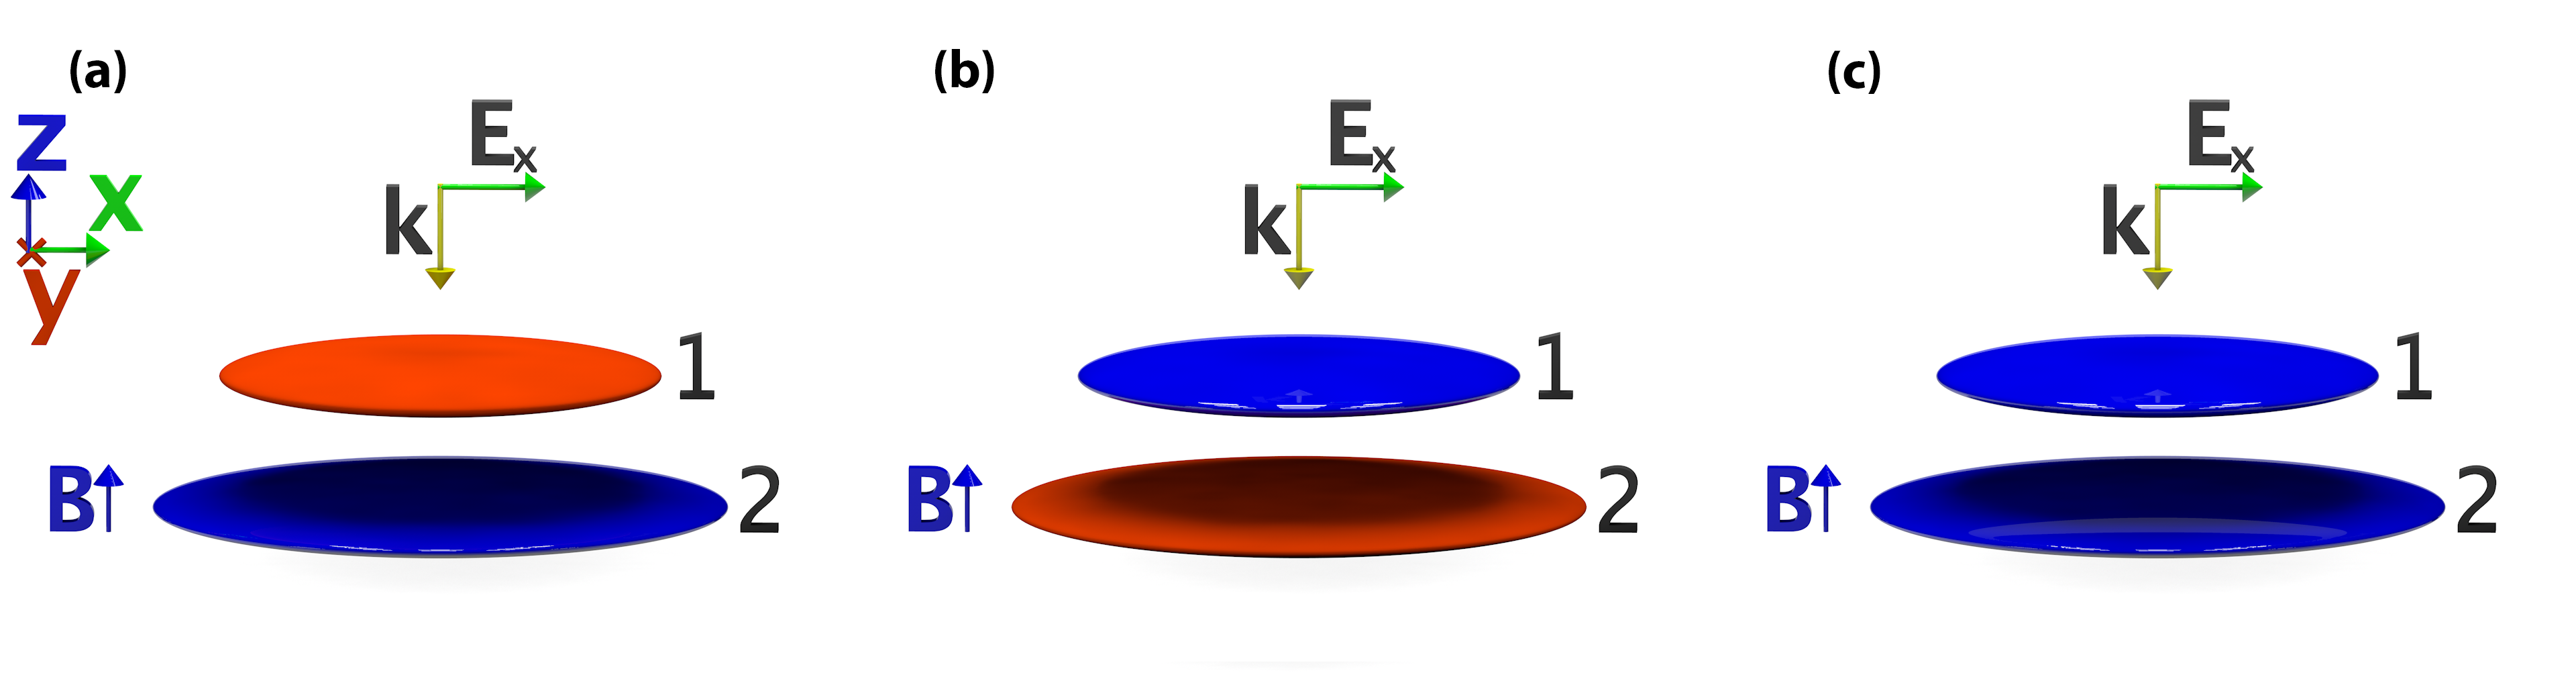
\includegraphics[width=1\columnwidth]{chapter_4/schemes/F1_join_aR1.png}
\caption{ Schematic representation of the studied configurations.\protect \\
 (a) The lower dipole is MP whereas the upper one is P, (b) the lower dipole is P whereas the upper disk is MP, (c) both disks are MP.\label{fig:chap5_schemetic_representation}}
\end{figure}


Since the actual fabricated structures have a truncated cone shape, the aspect ratio of the bottom dipole must be larger than that of the top one. For non-magneto-optical, plasmonic dipoles (P), we consider a diagonal, isotropic, dispersive dielectric tensor ($\textnormal{Au}$). For the magnetoplasmonic (MP) dipole, we consider an average medium that combines the dielectric tensor of a noble metal and that of a ferromagnetic one ($\textnormal{Au}$ and $\textnormal{Co}$ in this case), giving rise to a nondiagonal dielectric tensor. The nonzero off-diagonal elements depend on the relative orientation of the geometry, of the exciting radiation, and of the magnetic field as in the previous case. In our case, the external magnetic field is aligned perpendicular to the dipoles (\textit{i.e.}, aligned along the stacking direction; as schematically presented in Fig. (\ref{fig:chap5_schemetic_representation})), which corresponds to the so-called polar Kerr configuration, and the dielectric tensor of the MP dipole presents the form:

\noindent 
\begin{equation}
\boldsymbol{\epsilon}=\begin{pmatrix}\epsilon_{\text{d}} & \epsilon_{\text{M}} & 0\\
-\epsilon_{\text{M}} & \epsilon_{\text{d}} & 0\\
0 & 0 & \epsilon_{\text{d}}
\end{pmatrix}.\label{Tensor}
\end{equation}


Depending of the amount of $\textnormal{Co}$ within the MP disk, the elements of the dielectric tensor read as: 

\noindent 
\begin{equation}
\boldsymbol{\epsilon}_{\text{{d}}}=\left(1-\nu\right)\boldsymbol{\epsilon}_{\text{d,Au}}+\nu\boldsymbol{\epsilon}_{\text{d,Co}};\:\:\:\boldsymbol{\epsilon}_{\text{{M}}}=\nu\boldsymbol{\epsilon}_{\text{M,Co}}\label{Concent},
\end{equation}
 

where $\nu=\frac{V_{Co}}{V_{Co}+V{}_{Au}}$ is the $\textnormal{Co}$ relative amount in each dipole.

Once the dielectric tensor is known, we evaluate the static polarisability taking into account the properties of the particles, such as the shape (that in this case is oblate), material properties and dimensions. In order to conserve the energy, to the static polarisability is applied the radiative correction. The procedure used here is equivalent to the one presented in the previous chapter, in particular, we use Eq. (\ref{eq:chap3_polarizability}) and Eq. (\ref{eq:chap3_radiative_correction}) for polarisability and radiative correction respectively. \\

Knowing the polarisability for oblate particles, we are able to describe each disk as a single dipole. From coupled dipole theory, we know that the interaction between dipoles is mediated by the Green tensor $\mathbf{G}$. If an incident planar wave, with wave number $k$ and with electric polarisation in the plane of the dipoles, is used to excite the system (see Fig. (\ref{fig:chap5_schemetic_representation})) the two dipoles can be described in the $x-y$ plane as: 

\begin{eqnarray}
\mathbf{p}_{1} & = & \epsilon_{0} \boldsymbol{\alpha}_{1}\left[\mathbf{E}_{0,1}+\frac{k^2}{\epsilon_{0}}{G}\left(\mathbf{r}_{1},\mathbf{r}_{2}\right)\mathbf{p}_{2}\right]\nonumber \\
\mathbf{p}_{2} & = & \epsilon_{0} \boldsymbol{\alpha_{2}}\left[\mathbf{E}_{0,2}+\frac{k^2}{\epsilon_{0}}{G}\left(\mathbf{r}_{2},\mathbf{r}_{1}\right)\mathbf{p}_{1}\right],\label{Twodip}
\end{eqnarray}
which is the same equation obtained in the previous chapter. Due to the symmetry of the problem, the Green tensor is already defined in Eq. (\ref{eq:chap3_greenf}),  being $d$ the distance between dipoles, and $G\left(\mathbf{r}_{1},\mathbf{r}_{2}\right)$.\\


%\begin{eqnarray}
%G({\bf r}_{1},{\bf r}_{2}) & = & {G}({\bf r}_{2},{\bf r}_{1})=\mathcal{G}\mathbb{I}_{2\times2}=\frac{e^{ikr}}{4 \pi r}\left(\frac{(kr)^{2}+ikr-1}{(kr)^{2}}\right)\mathbb{I}_{2\times2},\nonumber \\
%\boldsymbol{\alpha}_{i} & = & \left(\begin{array}{cc}
%\alpha_{i} & \alpha_{iM}\\
%-\alpha_{iM} & \alpha_{i}
%\end{array}\right)
%\end{eqnarray}
The general solution of that system of equations under the influence of a plane wave linearly polarised along the $x-$axis and amplitude $E_{0}$ at dipole $1$ is given by:

\begin{eqnarray}
p_{1x}&=&\epsilon_{0}\frac{E_0}{\mathcal{D}}\left[\alpha_1+k^2 \mathcal{G}e^{-ikd}(\alpha_2\alpha_1-\alpha_{2M}\alpha_{1M})-k^4 \mathcal{G}^2\alpha_2D_1-k^6 \mathcal{G}^3e^{-ikd}D_1D_2\right]\nonumber\\
p_{2x}&=&\epsilon_{0}\frac{E_0}{\mathcal{D}}\left[e^{-ikd}\alpha_2+k^2\mathcal{G}(\alpha_2\alpha_1-\alpha_{2M}\alpha_{1M})-k^4\mathcal{G}^2e^{-ikd}\alpha_1D_2-k^6\mathcal{G}^3D_1D_2\right]\nonumber\\
p_{1y}&=&\epsilon_{0}\frac{E_0}{\mathcal{D}}\left[-\alpha_{1M}-k^2\mathcal{G}e^{-ikd}(\alpha_1\alpha_{2M}+\alpha_2\alpha_{1M})-k^4\mathcal{G}^2\alpha_{2M}D_1\right]\nonumber\\
p_{2y}&=&\epsilon_{0}\frac{E_0}{\mathcal{D}}\left[-e^{-ikd}\alpha_{2M}-k^2\mathcal{G}(\alpha_1\alpha_{2M}+\alpha_2\alpha_{1M})-k^4\mathcal{G}^2e^{-ikd}\alpha_{1M}D_2\right],
\label{eq:chap5_dipoles}\end{eqnarray}where $\mathcal{D}=1-2k^4\mathcal{G}^2(\alpha_2\alpha_1-\alpha_{2M}\alpha_{1M})+k^8\mathcal{G}^4D_1D_2$,
and $D_i=\alpha_i^2+\alpha_{iM}^2$. This equation is in fact a generalisation of Eq. (\ref{eq:chap3_polarizations_solution}). Note that the $y-$component of both dipoles is not zero when at least one of the dipoles is MO active.\\
For the particular geometry we are analysing, the external magnetic field produces a change in the polarisation state of the
reflected light, and the magneto-optical activity (MOA) of the whole system, defined as the modulus of the complex Kerr rotation, can be written as:

\begin{eqnarray}
\text{MOA}&=&|\theta+i\phi|=\textnormal{atan}\frac{\left|E_{y}^{R}\right|}{\left|E_{x}^{R}\right|}\approx\left|\frac{p_{1,y}+p_{2,y}}{p_{1,x}+p_{2,x}}\right|\nonumber \\ 
& = & \frac{(|p_{1,y}|^{2}+|p_{2,y}|^{2}+2|p_{1,y}||p_{2,y}|\cos(\Delta))^{\frac{1}{2}}}{(|p_{1,x}|^{2}+|p_{2,x}|^{2}+2|p_{1,x}||p_{2,x}|\cos(\Gamma))^{\frac{1}{2}}}.\label{CRot}
\end{eqnarray}

From the interaction point of view, there are three different regimes that are determined by the distance between the interacting dipoles: strong interaction (very close dipoles), weak interaction (very far away objects), and medium interaction (intermediate distance). We will concentrate on the most interesting case of medium interactions \cite{armelles2013mimicking}, and will analyse two situations: one in which the amount of $\textnormal{Co}$ in the magneto-optical disk is very small ($0.1\%$) and a second one where it is comparable to the $\textnormal{Au}$ amount ($25\%$). For the analysis, the aspect ratios of the dipoles are $a/c = 13$ and $10$ for the bottom and top dipoles, respectively.\\
\begin{figure}[h!]
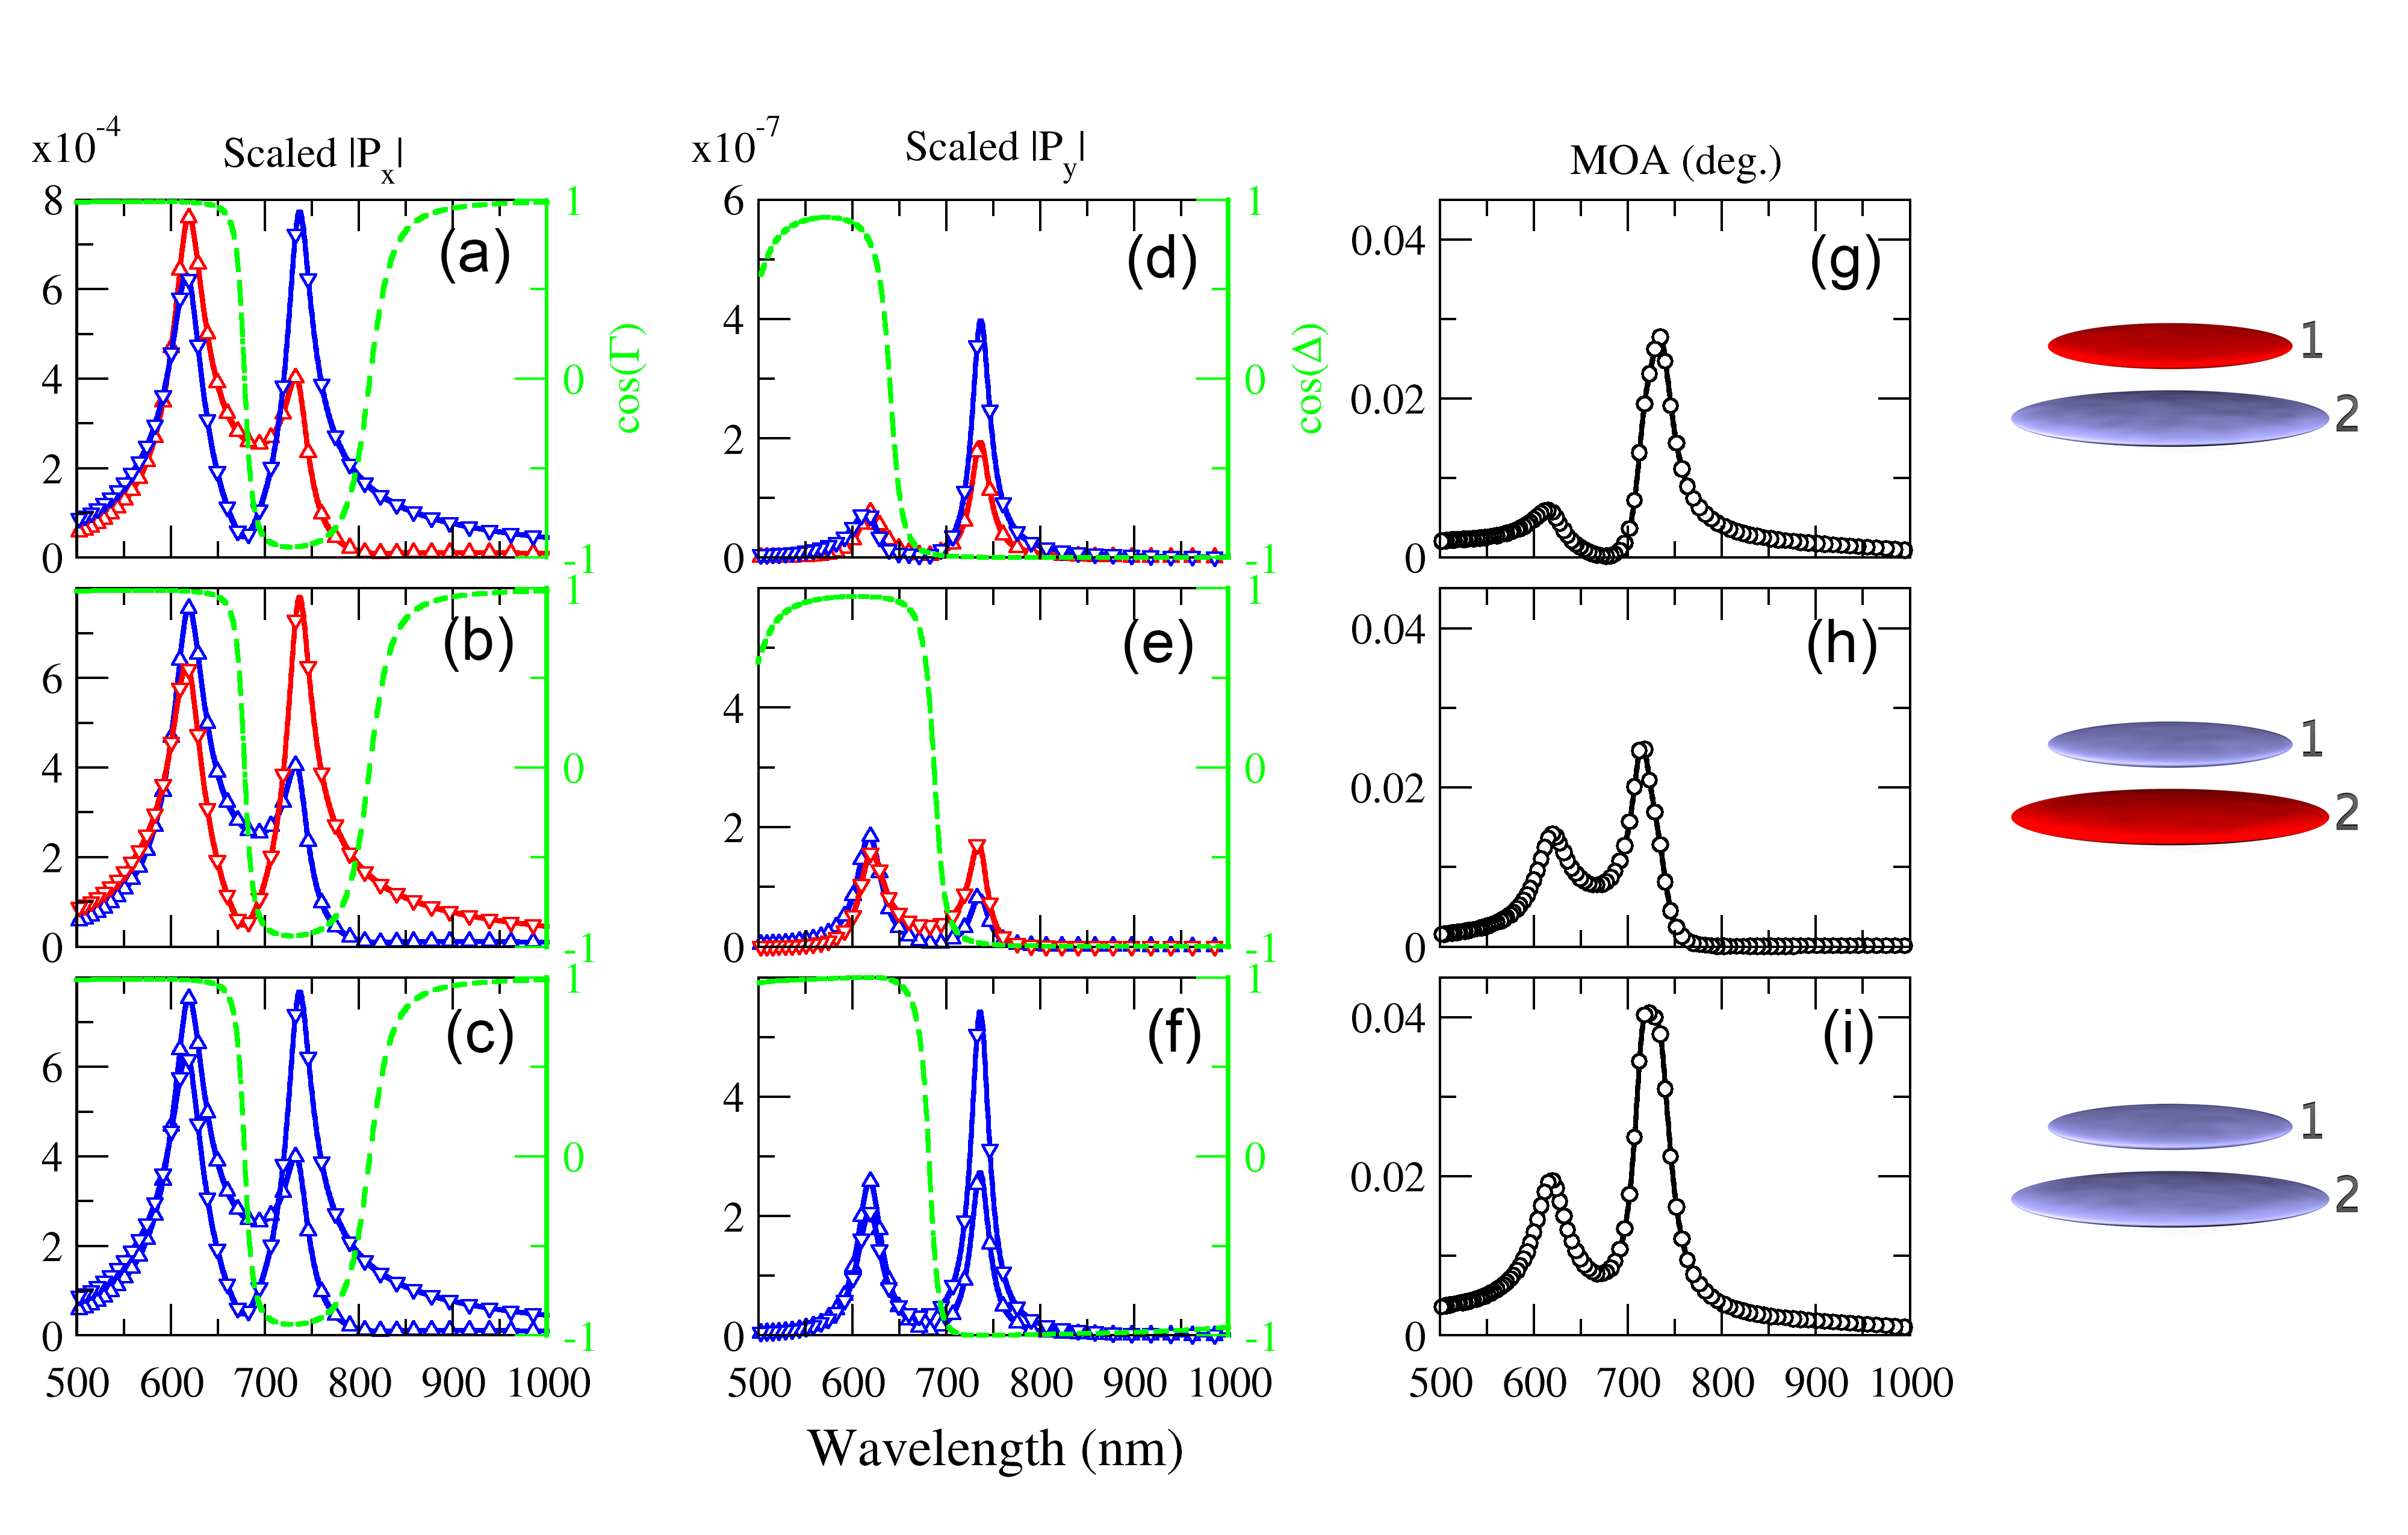
\includegraphics[width=1.0\textwidth]{chapter_4/graphics/F2_lowMO.png}
\caption{Dipole contributions, and MOA for 0.1\% Co concentration. (a)-(c) $x-$component of the scaled dipole (left axis) and the cosine of the relative phase between them (right axis), (d)-(f) $y-$component of the scaled dipole (left axis), and their relative phase (right axis), (g)-(i) magneto-optical activity. The upper panels represent the situation where the MP dipole is at the bottom, the medium panels are when the MP dipole is at the top, the lower panels when both are MP. Triangle-up for the top dipole, and triangle down for the bottom dipole.\label{LowInt}}
\end{figure}
Let us start with the case of very small $\textnormal{Co}$ concentration ($0.1\%$) in the MP dipole. In Fig. (\ref{LowInt}), we show the modulus of the components of the dipole along $x$, the polarisation direction of the incident beam ($p_{i,x}$), and along the $y-$direction ($p_{i,y}$), as well as that of the complex Kerr rotation (MO activity, MOA) calculated with this simple analytical model for the situations where the MP dipole is at the bottom, top, and in both positions of the structure. The cosine of relative phases between the $p_{i,x}$, $\cos\Gamma$ presented in Figs. \ref{LowInt}(a)-\ref{LowInt}(c), and $p_{i,y}$, $\cos\Delta$ presented in Figs. (\ref{LowInt})(d)-(\ref{LowInt})(f), components of the upper and lower disks (dashed curves) are also shown, with limit values of $1$ and $-1$ for in-phase and out-of-phase oscillations, respectively.\\
Considering first the $x-$component of the dipoles, shown in Figs. (\ref{LowInt})(a)-(\ref{LowInt})(c), and due to the low $\textnormal{Co}$ concentration, there is no noticeable difference between the three situations. All cases show two characteristic low-energy ($740nm$) and high-energy ($620nm$) modes of antisymmetric and symmetric nature, respectively \cite{dmitriev2007gold,armelles2013mimicking,banthi2012high}, as directly concluded by the obtained relative phase between the two dipoles. The abrupt change in sign of the cosine occurs exactly at the minimum in magnitude of both dipoles. For energies below roughly $760nm$, the phase gradually changes again, going back to an in-phase configuration for wavelengths larger than $820nm$. Regarding the relative contribution of both disks to these $p_{x}$ spectral features, the low-energy mode has a stronger component originating from the bottom disk (down triangles) than from the top one (up triangles), since it has a lower aspect ratio. The situation is reversed for the high-energy peak, even though the difference between the contributions of the two dipoles is smaller.\\
Beyond the purely optical properties, fully understandable by simply considering $p_{x}$, the direct consequence of the application of a magnetic field is the generation of a $y-$component in the dipole \cite{sepulveda2010plasmon,armelles2013mimicking} (Fig. (\ref{LowInt})(d)-(f)). Contrary to what is observed in the $x-$component, now different results are obtained depending on the specific position of the MP-active dipole.\\
Let us examine each situation individually. When the MP dipole is at the bottom, a $y-$component is observed not only in this dipole, but also in the P top one, which is due to the interaction between the dipoles. This $y-$component is stronger for the bottom MP dipole in the low-energy region, but they are similar in the high-energy region. Even more, in the spectral region, where the $x-$component of the MP dipole is minimum, the $y-$component of both dipoles is almost zero, even though the $x-$component of the P dipole in the same intermediate region is not negligible. This is simply due to the fact that the $y-$component is originated by the magnetic-field-induced rotation of the MP dipole, which in turn induces the rotation of the upper P dipole. Thus, a $y-$component dipole can be originated only if the $x-$component of the MP active dipole is not zero. Additionally, the relative phases between the two dipoles along the $y$ axes show essentially the same symmetric/antisymmetric configuration for the corresponding high/low-energy modes compared to those for the $x-$components, even though now they do not return to in-phase values for energies below $800nm$. The presence of $p_y$ is directly related to the presence of MO activity in the system (see Fig. (\ref{LowInt})(g)). Indeed, as shown in Eq. (\ref{CRot}), this magnitude is basically the modulus of the sum of the $y-$components of the top and bottom dipoles divided by that of the $x-$components. Therefore, the spectral dependence of MOA can be understood in simple terms considering these four dipole components, taking into account their relative phases. So, in this first considered case with the bottom MP dipole, the high-energy peak results from the addition of both (top and bottom dipoles) $y-$components, while the low-energy one results from the corresponding difference, since in this energetic range the $y-$components are in phase opposition.\\
If we consider now the situation where the MP dipole is on the top of the structure, the results are very different. Strikingly, here the obtained $y-$component in the low-energy region is larger for the P dipole than for the MP one, while both components are similar for the high-energy region. This means that the contribution to the MOA coming from the P dipole in the low-energy region is actually stronger than that of the MP one, as shown in Fig. (\ref{LowInt})(h). This is simply due to the larger $x-$component of the P dipole in the low-energy region, which also explains why the $y-$components in the high-energy region are of similar magnitude for both the MP and P dipole in the previous case. On the other hand, regarding the intermediate spectral region, and due to the nonvanishing $x-$component of the MP dipole in this range, both the $y-$components (especially of the P dipole) and the MOA are not zero.
Finally, if both disks have an MO component, the intensity of the $p_y$ components increases for both dipoles, and, within each mode, they follow the same trend as the corresponding $x-$component. Besides, for all of the energy regions, the  intensity of the MOA is larger than that of the other two configurations. 

\begin{figure}
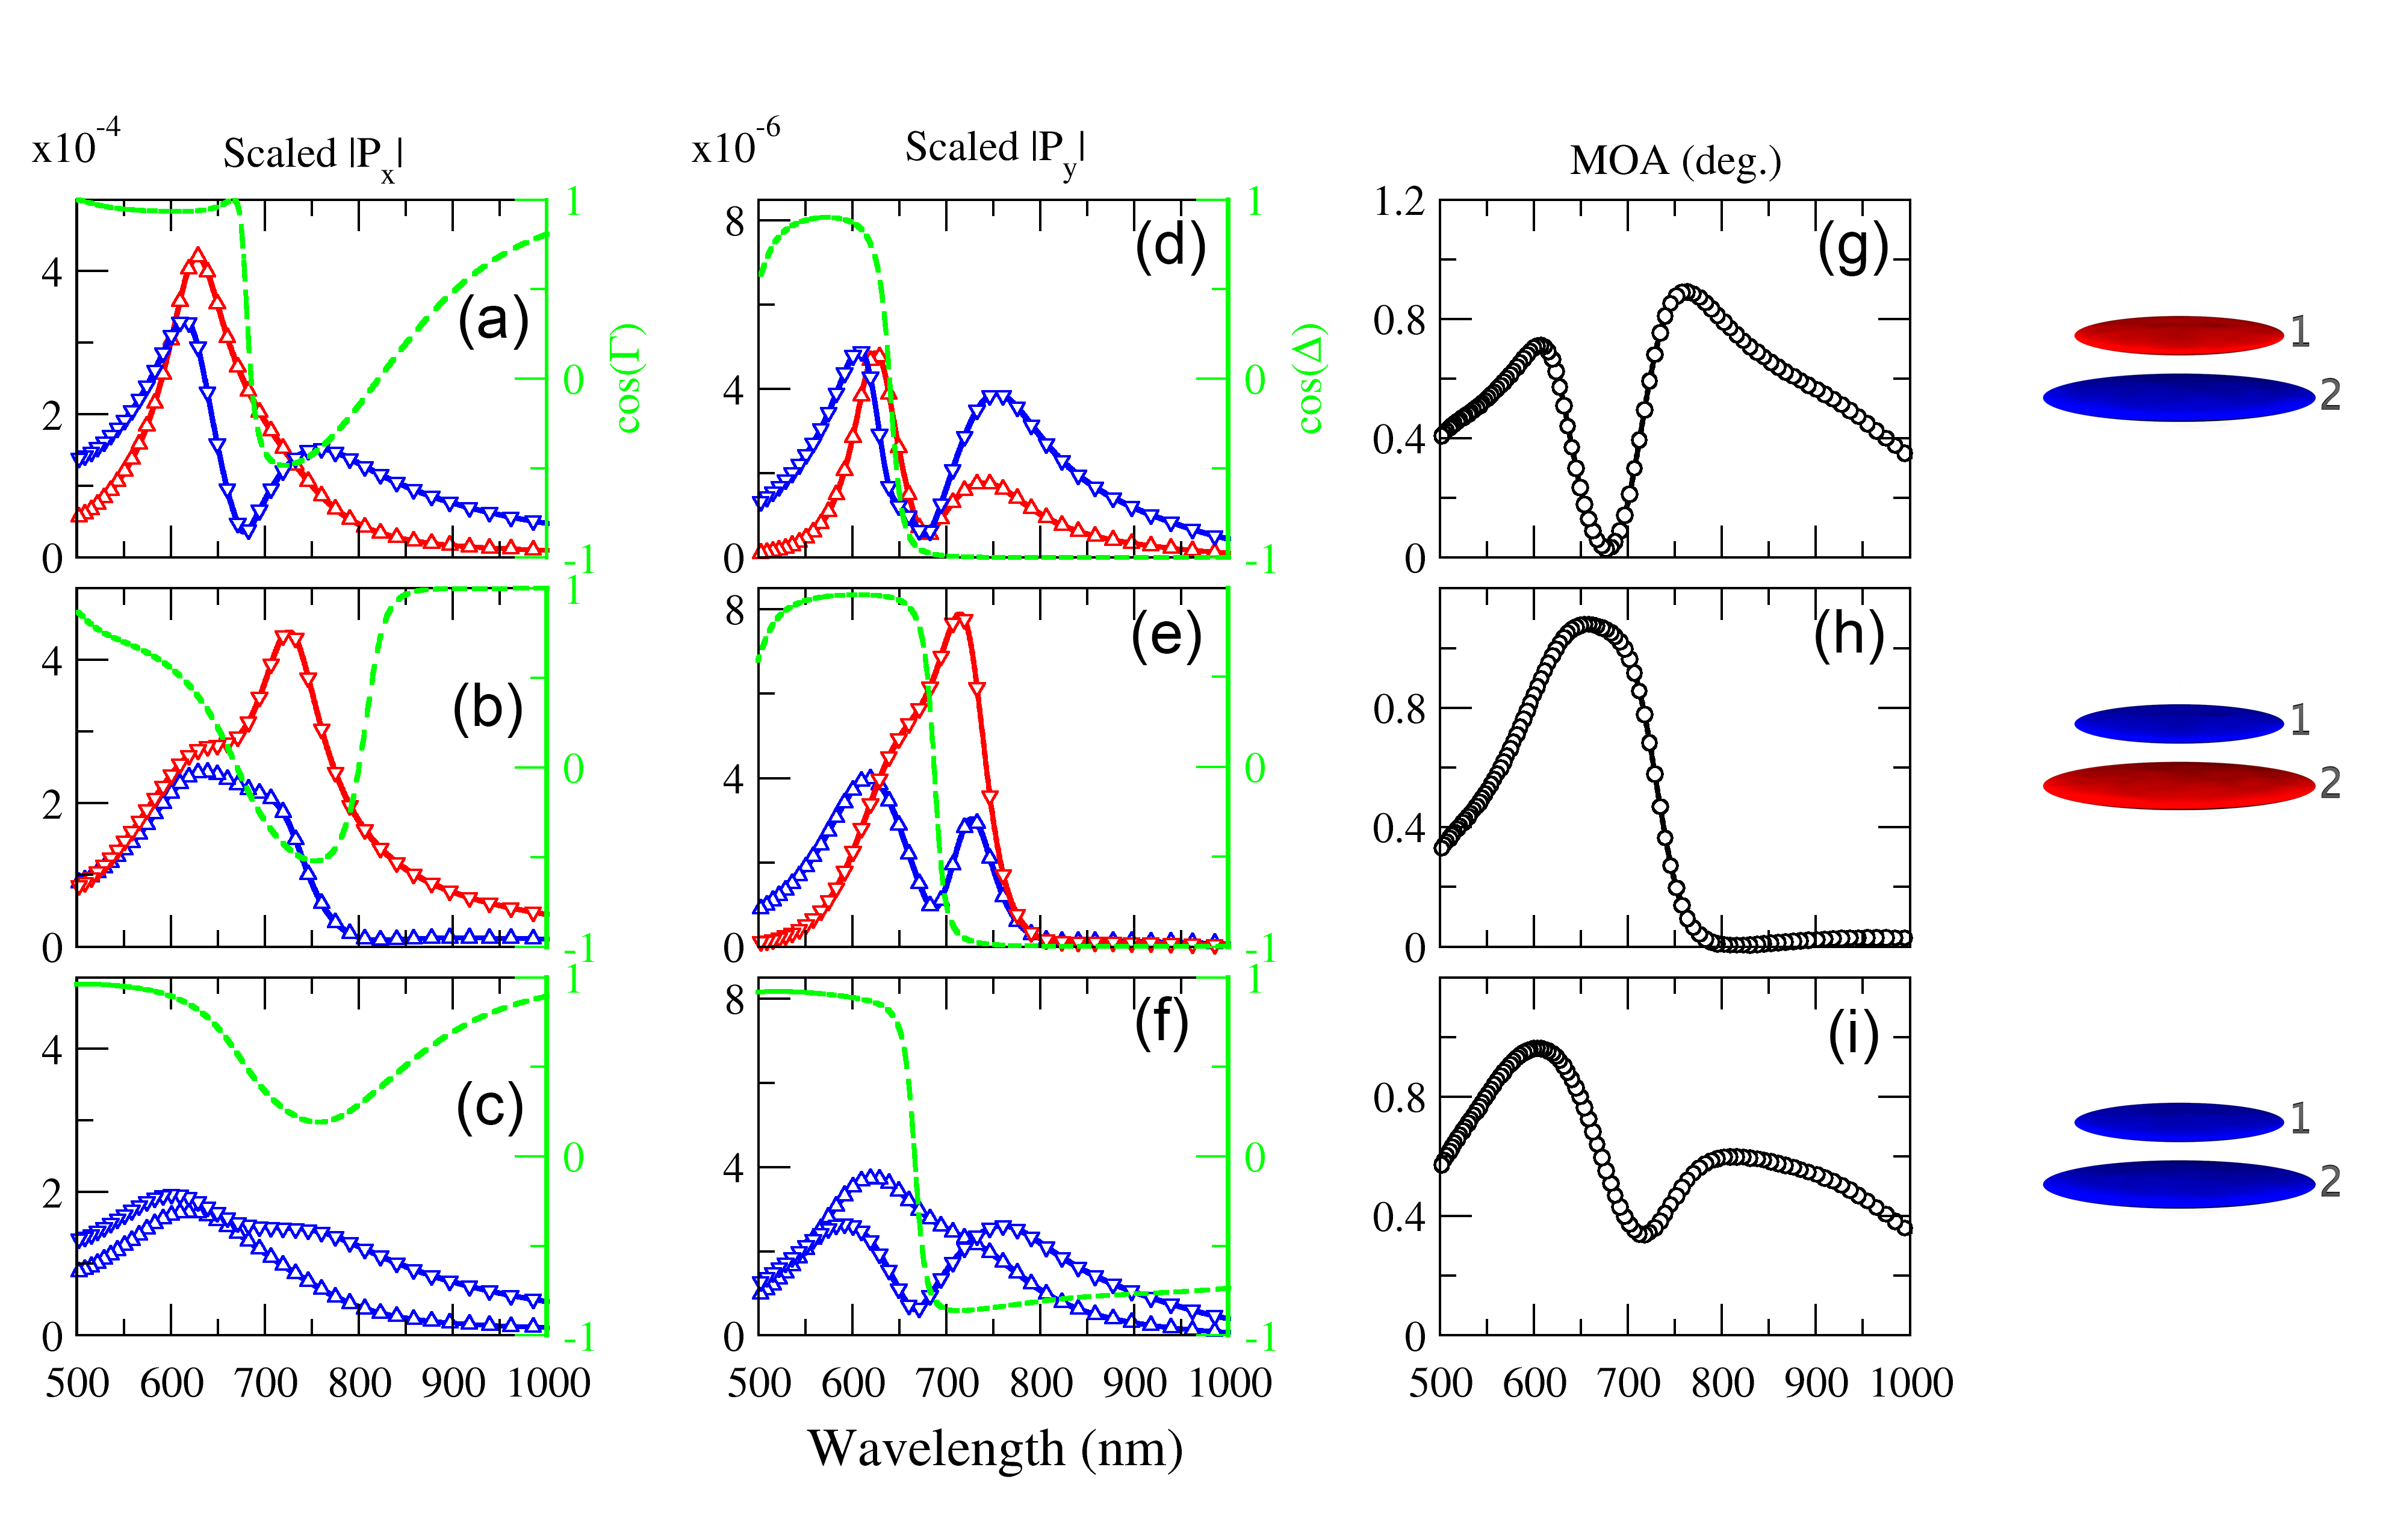
\includegraphics[width=1\textwidth]{chapter_4/graphics/F3_highMO.png}

\caption{Dipole contributions, and MOA for 25\% $\textnormal{Co}$ concentration. (a)-(c) $x-$component of the scaled dipole (left axis) and the cosine of the relative phase between them (right axis), (d)-(f) $y-$component of the scaled dipole (left axis), and their relative phase (right axis), (g)-(i) magneto-optical activity. The upper panels represent the situation where the MP dipole is at the bottom, the medium panels are when the MP dipole is at the top, the lower panels when both are MP. Triangle-up for the top dipole, and triangle down for the bottom dipole \label{HighInt}}
\end{figure}

Going towards a more realistic situation, with larger $\textnormal{Co}$ amounts in the MP dipoles, in Fig. (\ref{HighInt}) we show theoretical calculations equivalent to those shown in Fig. (\ref{LowInt}) but using the dipole model with a $25\%$ $\textnormal{Co}$ content in the different MP dipoles. As can be seen in Figs. (\ref{HighInt})(a)-(\ref{HighInt})(c), and contrary to what was observed for low $\textnormal{Co}$ concentrations, now the $p_x$ components are very different depending on the specific position MP dipole. The effect of increasing the $\textnormal{Co}$ amount is both to broaden the peaks and to change their absolute and relative intensities, as well as their energetic position, both for $p_x$ and $p_y$ components. Due to the much larger amount of $\textnormal{Co}$ ($250$ times more $\textnormal{Co}$) in this case, the magnitudes of the $p_x$ and $p_y$ components are now very different (between a factor of $2$ to $4$ reduction in the $x-$component due to the increased losses, and roughly one order of magnitude larger in the $y-$component due to the much larger amount of MO material). Even more, for this concentration, all of these effects also depend on the specific location of the MP dipole.\\
For the configuration with the MP dipole at the bottom, the low-energy peak in the MOA has a stronger component due to the bottom dipole (as seen in the low $\textnormal{Co}$ concentration case) and the increase of the $\textnormal{Co}$ amount brings, as a consequence, both a reduction of the relative intensity for the $x-$component and a broadening for both the $x-$ and $y-$components. However, the high-energy peak, with a stronger contribution from the upper P dipole, is less affected since no $\textnormal{Co}$ is present in it. Again, a minimum in the $y-$component in the intermediate-energy region yields a minimum in the MO activity. Regarding the relative phases, for the $p_x$ components, it is clear now that they do not reach the perfect out-of phase configuration, indicating that now the nature of the modes is not purely but only partially antisymmetric. This is due to the sizable amount of $\textnormal{Co}$ present in the dipoles, which enhances the losses of the system and affects the retardation between the two coupled dipole $x-$components. However, for the $y-$components, the phase basically reproduces the same behaviour observed for the very low concentration limit.\\
Going now to the situation where the MP dipole is in the upper part, the most affected peak (for all $p_x$, $p_y$, and MOA) due to the incorporation of $\textnormal{Co}$ is the high-energy one, since it is the one which carries a stronger part of the upper dipole. We therefore observe a change in the relative intensity with respect to the case with the MP dipole in the bottom. Remarkably, in this situation, the $y-$component of the P dipole is much larger than that of the MP one in the low-energy part of the spectrum, due to the interaction effects and to the very large $x-$component of this P dipole. Now, due to both the broadening and spectral overlapping of the $y-$components of both top and bottom dipoles, only one broad peak is observed in the MOA. This peak is mainly originated by the induced $y-$component in the bottom dipole, which is not MO active. Regarding the phase of the $y-$component, it is worth noticing that it is again exactly the same as for the low $\textnormal{Co}$ concentration, \textit{i.e.}, it does not depend on the $\textnormal{Co}$ concentration. If one considers Eq. (\ref{eq:chap5_dipoles}), makes either $\alpha_{1M}$ or $\alpha_{2M}$ equal to zero, the ratio between the $y-$components of the P and MP dipoles becomes $p_{y,\textnormal{NMO}}/p_{y,\textnormal{MO}}=k^2\mathcal{G}\alpha_{\textnormal{NMO}}$, \textit{i.e.}, it does not depend on the MO active element, and thus the relative phase does not depend on the $\textnormal{Co}$ content.\\
Finally, when both dipoles are MP, the larger amount of $\textnormal{Co}$ implies that the total losses are even larger, and therefore the peaks in the $x-$components are weaker and broader. The direct consequence of this reduction in the $x-$components is that the $y-$components are also somehow weaker and broader compared to the other two cases with only one MP dipole. Now, for the $x-$component, the two peaks overlap for the bottom dipole and only one broad peak is observed for the top one, which is also the same behaviour basically observed for the $y-$component. Regarding the MOA, two very distinguishable peaks are observed and, surprisingly, the low-energy one yields lower MO activity than the corresponding peak for the other two cases (only one MP dipole), contrary to what was observed for low $\textnormal{Co}$ concentration. This is due to the smaller difference of intensities between the $y-$components of the two dipoles in this case and to the fact that in this spectral region, they are out of phase. Briefly, this complex behaviour of relative intensities and phases induces a smaller MOA even when more MP components are present in this dimer.\\
Let us summarise the preceding discussion. When two dipoles interact, with one of them presenting MO activity (MP dipole), this MP dipole can induce MOA in the non-MO-active (purely plasmonic, P) one. The induced MOA can even be much larger than the intrinsic one, as seen in the low-energy region of Figs. \ref{LowInt}(e) and \ref{HighInt})(e). This occurs in the spectral region of the resonance of the P dipole. On the other hand, if the system is composed of two MP, lossy dipoles (high $\textnormal{Co}$ content), the resulting MOA response can be much lower than that obtained when only one dipole is MP, shown in Figs. (\ref{HighInt})(g)-(\ref{HighInt})(i)]. This has important consequences in real magnetoplasmonic systems composed of noble metals and ferromagnetic metals. One would naively think that the MOA would be enhanced increasing the number of MP components, but then the losses will increase in parallel. Our results show that an adequate stacking of the system components may allow devising structures with higher MO activity using overall lower amounts of ferromagnetic content.


\section{Full numerical calculations and experimental results}

\begin{figure}
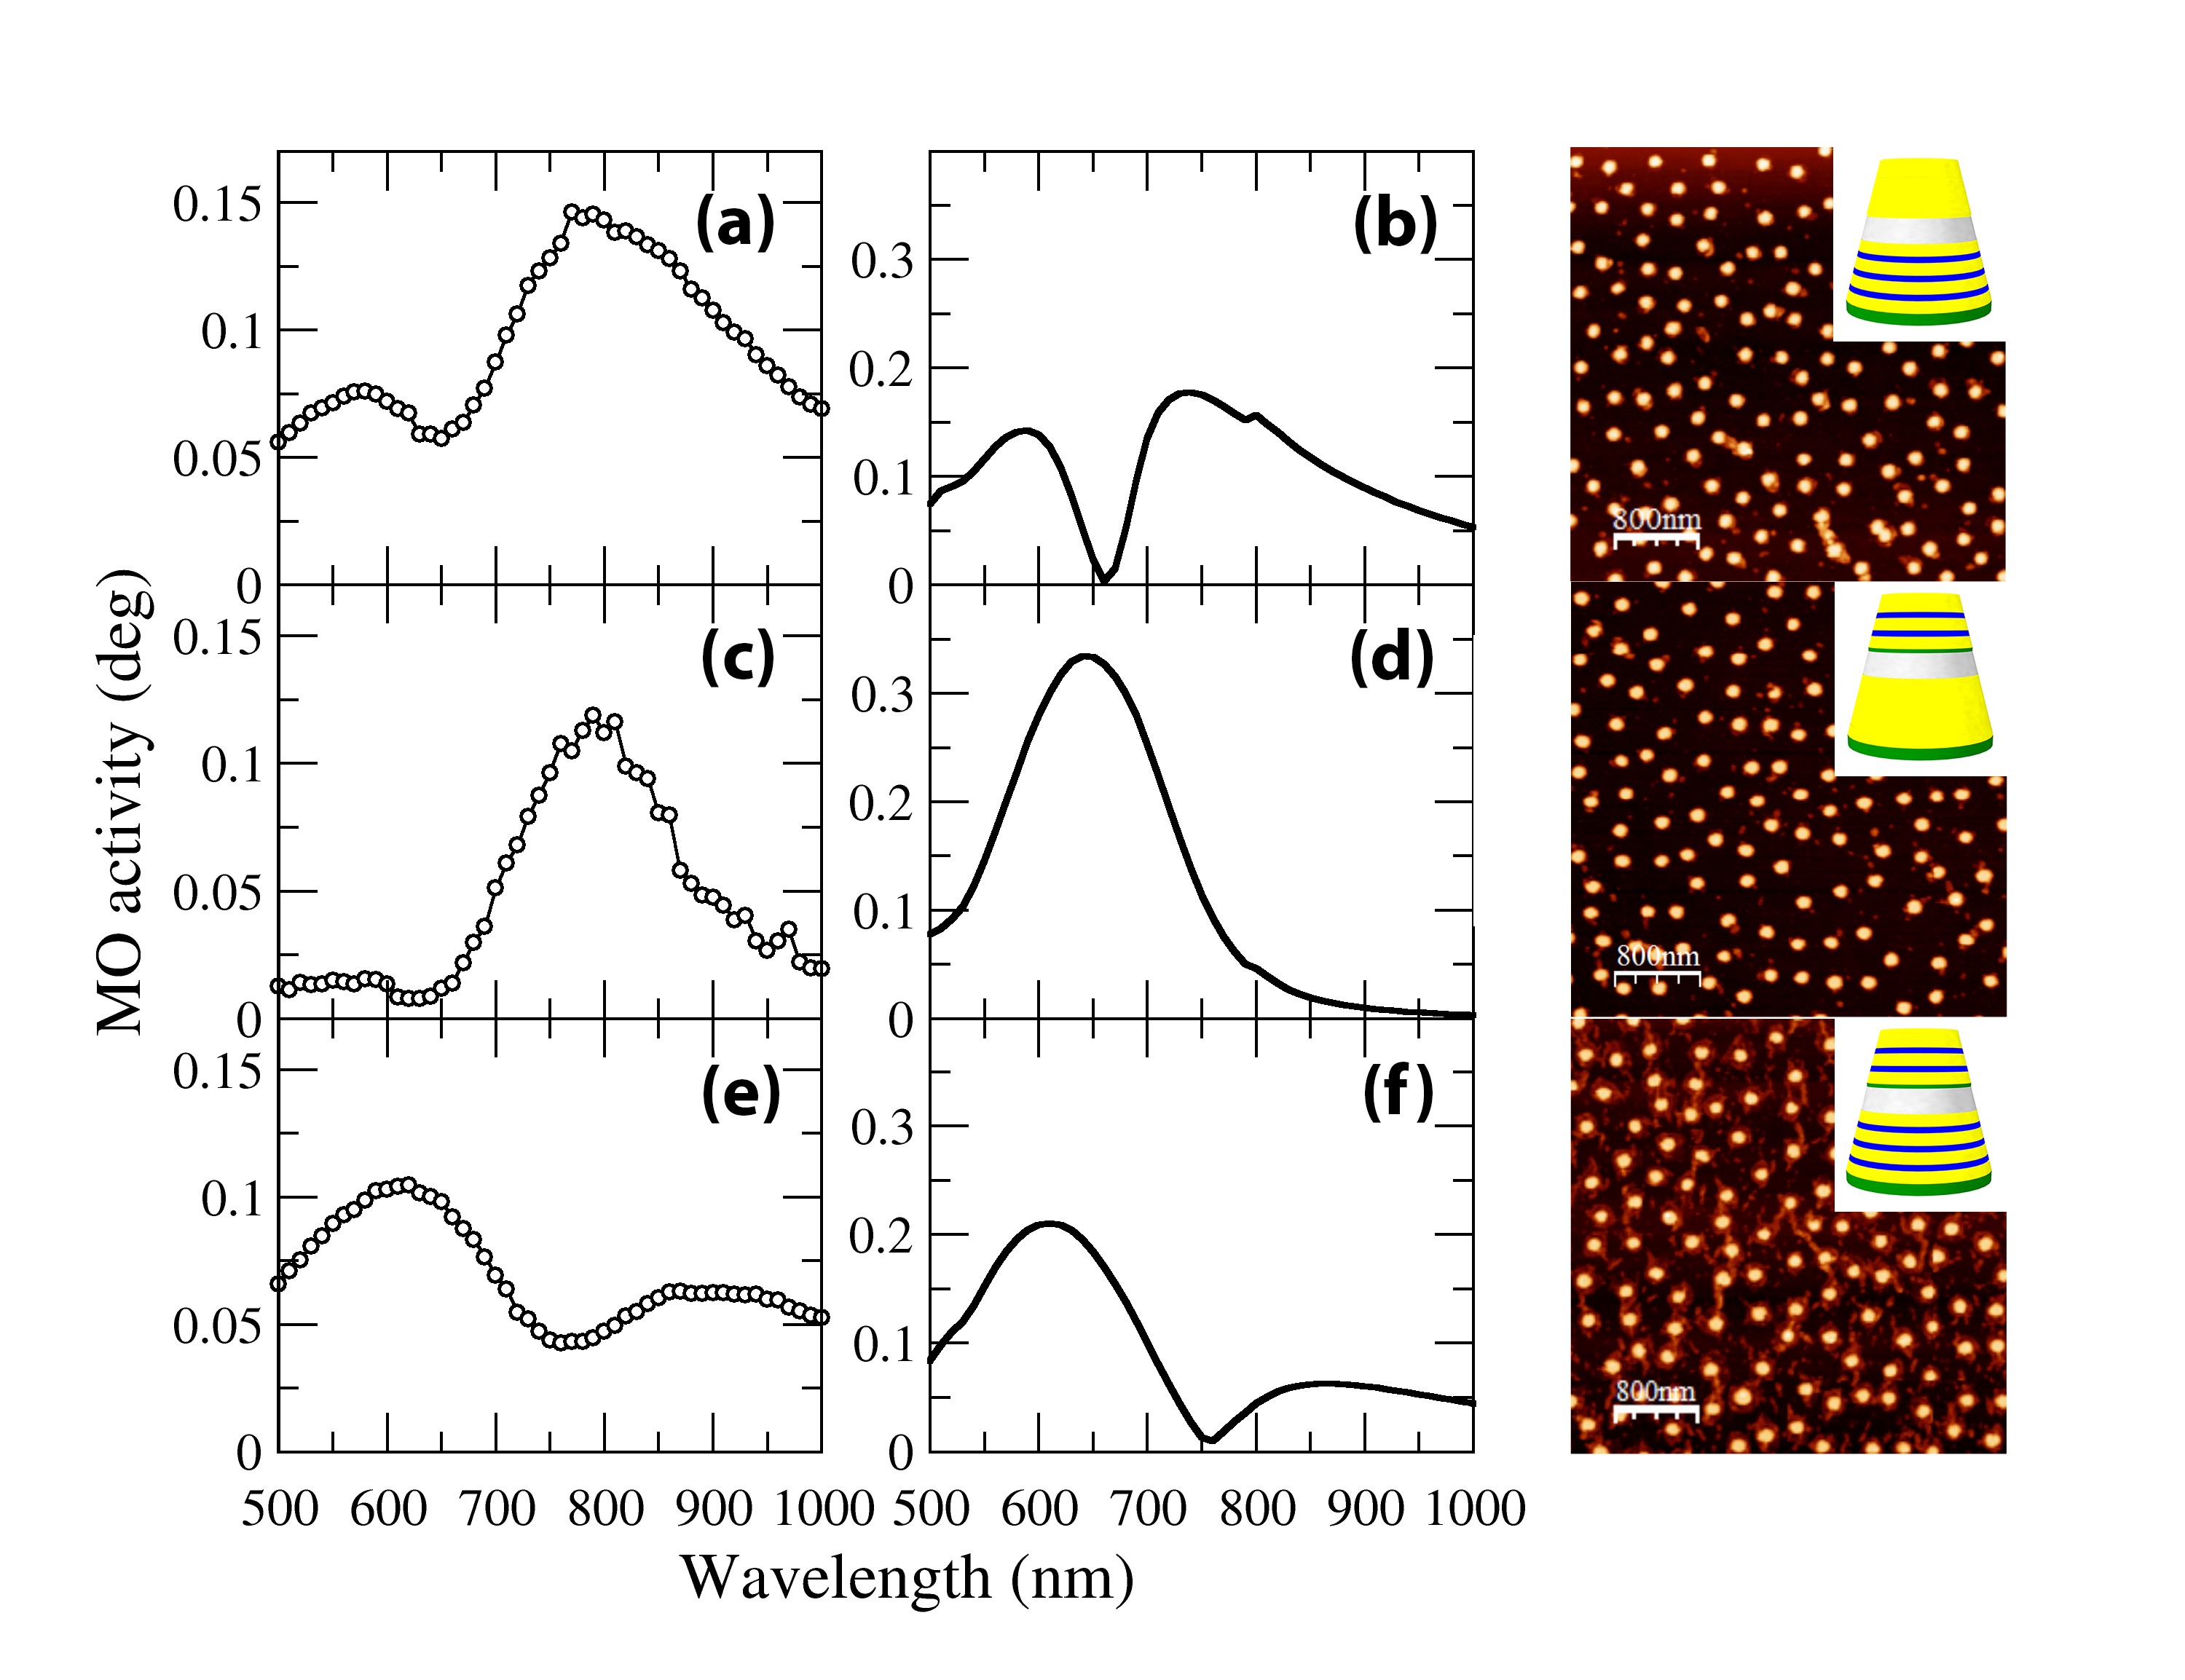
\includegraphics[width=1\columnwidth]{chapter_4/graphics/F4_MOA_3x3_finalR1.png}
\caption{Experimental results (a) and numerical simulations (b) of the MO activity when the MP disk is at the bottom, (c),(d) are the same but when the MP disk is at the top, and (e),(f) when both are MP. In the rightmost panel we show Atomic Force Microscopy (AFM) images of the three experimental samples where the density of disks (about $15\%$ coverage) and homogeneity can be seen. The images show that the disk diameter ranges from $130nm$ to $150nm$. Also is represented a scheme of the structures. In green we depict the $\textnormal{Ti}$ adhesive layer, in blue the $\textnormal{Co}$ layers, grey is the $\textnormal{SiO}_{2}$ and yellow are the gold layers. The three different systems are constituted by two metallic disks separated by $20nm$ of $\textnormal{SiO}_{2}$. For the configuration with the MP disk at the bottom (top panels), the MP disk is composed of a $2nm$ $\textnormal{Ti}$ layer followed by a $4nm$ $\textnormal{Au}$ layer and three sequential combinations of $2nm$ $\textnormal{Co}/4nm$ $\textnormal{Au}$ layers. The disk at the top is composed by $16nm$ $\textnormal{Au}$. For the configuration with MP disk at the top, the MP disk is composed by an initial $1nm$ layer of $\textnormal{Ti}$ then $4nm$ $\textnormal{Au}$ layer and two sequences of $2nm$ $\textnormal{Co}/4nm$ $\textnormal{Au}$ layers. The disk at the bottom is composed by $22nm$ of $\textnormal{Au}$. When both disks are MP, they consist of those $\textnormal{Au}/\textnormal{Co}$ sequences employed in the other two situations. \label{chap5:Experim}}
\end{figure}

Despite the simplicity of the two interacting dipoles model, it describes quite well the outcome of the interaction between disks in magnetoplasmonic dimers. For example, in Fig. (\ref{chap5:Experim}), we present the experimental MO activity for three different samples. They consist of a layer of two metallic disks separated by $\approx 20 nm$ of $\textnormal{SiO}_2$.  deposited on a glass substrate. The three samples have a homogeneous distribution of the disks, with a filling factor of $15\%$. The diameter of the disks ranges from $130$ to $150nm$. They were obtained by hole mask colloidal lithography, metal evaporation, and lift off \cite{fredriksson2007hole}. The internal structure of the disks is presented in the rightmost panel of Fig.  (\ref{chap5:Experim}), with the disk's dimensions in the caption. In the upper panel, the bottom disk consists of a $\textnormal{Au}/\textnormal{Co}$ multilayer (MP) and the top one is a $\textnormal{Au}$ disk (P); in the middle panel, the top disk is a $\textnormal{Au}/\textnormal{Co}$ multilayer (MP) and the bottom one is a $\textnormal{Au}$ disk (P); and, finally, in the lower panel, both disks are $\textnormal{Au}/\textnormal{Co}$ multilayers (MP).\\
As can be observed, when the bottom disks are magnetoplasmonic, \textit{i.e.}, upper and lower panels on the righthand side of Fig. (\ref{chap5:Experim}), the MOA spectrum has two peaks. Despite the lower $\textnormal{Co}$ content of the upper panel, the lower-energy peak has a higher intensity in this sample than in the lower panel, where the two disks are magnetoplasmonic. Moreover, the MOA spectrum of the middle panel has only one peak, whose intensity is also greater than the intensity of the low-energy peak of the lower panel. Additionally, in Fig. (\ref{chap5:Experim}), we also present a FDTD theoretical calculation which takes into account the internal structure of the disks. As can be observed, these calculations reproduce quite well the experimental behaviour, and the results are also equivalent to those obtained with the previously exposed analytical approach for intermediate interactions presented in Fig. (\ref{HighInt}). The numerical calculations have been made using $130nm$ for the diameter of the base of the cone and $100nm$ for the top in all cases. An increase in these numbers would cause a redshift of the peaks.

\section{Conclusion}

In conclusion, we have analysed the effect of electromagnetic interactions on the MO response of magnetoplasmonic dimers composed of two metallic disks separated by a dielectric. The MO response strongly depends on the plasmonic versus magnetoplasmonic nature of the two disks, observing for specific configurations that the MO response can be dominated by the induced MOA of the purely plasmonic disk. On the other hand, the MO activity of a system with only one of the disks containing material with intrinsic MO can be even larger than that of a system composed of two MP disks. A simple analytical model of two interacting point dipoles allows us to fully describe separately the contribution of each disk to the optical and MOA of the system, along with the relative phases of the dipoles responsible for these activities. Experimental results and numerical calculations fully support the analytical calculations results.


%\bibliographystyle{plain}
%\bibliography{References}                                   %Chapter 4
\chapter{Magnetically controlled optical nanoantennae\label{chap5}}

\section{Introduction}

%In Feynman's seminal talk about control and manipulation of matter at nanoscale\footnote{Richard Feynman, \textit{There's plenty of room at the bottom},  at the Annual Meeting of American Physical Society (1959):\\ "Consider, for example, a piece of material in which we make little coils and condensers (or their solid state analogs) 1,000 or 10,000 angstroms in a circuit, one right next to the other, over a large area, with little antennae sticking out at the other end-a whole series of circuits. Is it possible, for example, to emit light from a whole set of antennae, like we emit radio waves from an organised set of antennae to beam the radio programs to Europe? The same thing would be to beam the light out in a definite direction with very high intensity. (Perhaps such a beam is not very useful technically or economically."} \cite{Feynman_1960}, he suggested that, like matter, light could also be handled at small sizes. 60 years later, this prediction was only possible due to the extensive work in near-field optics \cite{Novotny_PNO_2012,Biagioni_2012}.\\
Over the last two decades there has been a boost in nanoantenna research, mainly due to the possibility of create structures at nanoscale. Improvements in fabrication techniques, like electron-beam lithography \cite{ghenuche2008spectroscopic,Schuck_2005,Muskens_2007}, focused ion-beam milling \cite{muhlschlegel2005resonant,Farahani_2005,Kim_2008}, nano-imprinting lithography \cite{Boltasseva_2009} or positioning of nanoantennae on tips \cite{Anger_2006}, etc., made possible the use of nanoantennae in near-field optical spectroscopy \cite{Nie_1997,Hartschuh_2003}, single-photon superemitters \cite{Kim_1999,Michler_2000, Lounis_2000}, optical tweezing \cite{Zhang_2010, Grigorenko_2008}, or microscopy \cite{Betzig_1993, Frey_2004}, among others.\\
At nanoscale, light can be controlled and manipulated using electromagnetic sources like fluorescent molecules, quantum dots, etc., usually coupled to an external structure that operates as an antenna. These nanoantennae, from the viewpoint of its operation, are similar to telecommunication antennae \cite{Pohl_2000}. 
%Its function consists in the presence of free charge carriers confined in well-defined regions of space. When applied an oscillating potential, the charges start to move, generating an electromagnetic field \cite{Jackson_CE}. 
In order to obtain optical wavelengths is necessary to reduce the antenna dimensions \cite{Kawata_2011}.\\
%A fundamental electromagnetic source is an oscillating dipole, initially proposed by Hertz \citep{Bryant_1988} as two opposite charged spheres connected by a metallic wire. When left alone, the system tends to the equilibrium, generating an exponentially damped harmonic oscillator at frequency $\omega_{0}=1/\sqrt{LC}$, for a small damping, with $L$ the inductance and $C$ the capacitance of the system. The exponential damping has its origins in the Ohmic resistance felt by the charge carriers in the metal wire and the loss energy due to radiation of electromagnetic waves. 
%In order to obtain radiation at optical frequencies, is necessary to reduce $L$ and $C$, or from the practical point of view, is necessary to reduce the antenna dimensions \cite{Kawata_2011}.\\
%Metallic nanoantennae, at optical frequencies, cannot be considered as perfect conductors. With the frequency increasing, electrons react with an amplitude increasing and phase lag to the oscillating electromagnetic field, due to the effective mass of the electrons. When the phase lag approaches $90^{\circ}$, the amplitude reaches a maximum that is only constrained by the damping. This plasmon resonance is function of the intrinsic properties of the nanoantenna like material properties (only occurs in metallic particles), geometric shape and size.\\
Many different types of nanoantennae have been proposed and experimentally investigated \cite{pelton2008metal, novikov2014gold}. Studies with single nanospheres \cite{Wang_2006, chen2011plasmonic} and nanorods \cite{Bryant_2008} show the possibility of tuning the resonance frequency considering the size and aspect ratio of the particles. Dimers of nanospheres \cite{Rechberger_2003} and nanorods \cite{Muskens_2007} can be used to enhance the near-field intensity at some space positions. Bow-tie dimer nanoantennae are being applied to enhance molecular fluorescence \cite{Farahani_2005,Kinkhabwala_2009}, Raman scattering \cite{Fromm_2006} and for high-harmonic generation \cite{Kim_2008}. With the aim of redirect the field like in telecommunication antennae, Yagi-Uda antennae \cite{taminiau2008enhanced, Kosako_2010} have been proposed and implemented, as well as anisotropic emitter-antenna coupling systems \cite{Taminiau_2008}. \\
One subject that has attracted attention recently has been the control of nanoantennae via an external parameter, as in the previous chapters.
%In this chapter we propose an optical nanoantenna where its response is modulated by an external parameter \cite{Krasavin_2004}.
A possibility is to consider the use of a static magnetic field \cite{armelles2013magnetoplasmonics}. \\
%It has been already mentioned that magneto-optics have received attention recently due to the possible applications, such as nonreciprocal optical isolators \cite{van2006transverse, dotsch2005applications, espinola2004magneto}, sensors \cite{sepulveda2006highly}, plasmonic interferometry \cite{martin2010enhancement, martin2013plasmonic}, random-lasers \cite{pinheiro2008statistics}, etc.\\
Also in Sec. (\ref{chap2:Dipole_radiation}) we presented the Purcell effect \cite{Purcell_1946}, where the modification of the lifetime of an emitter by shaping the electromagnetic environment is reported. 
%A special look should be given to the work of Marinchio \textit{et al.} \cite{marinchio2012light}, where was studied the interaction of a magneto-optical nanoparticle in the presence of a flat surface. In this work was shown that the magneto-optical contribution in the dressed polarisability could be enhanced. 

In this chapter we study the properties of an emitter in two different situations: in the presence of a single magnetoplasmonic (MP) nanoparticle, Sec. (\ref{sec:chap5_singlepart}), and inside of a cavity formed by two MP nanoparticles, Sec. (\ref{sec:chap5_cavity}).\\
We consider a simple model where particles are described as dipoles, and consequently characterised by its polarisabilities, in which the interaction between the elements is governed by the dipole-dipole coupling. This choice is motivated by the possibility of obtain simple analytical expressions that could capture the physics of the problem.\\
We analyse the dependence of the emitter decay rate and the radiated field patterns by the system \textit{emitter and nanoparticle(s)} as a function of the distance between the emitter and the nanoparticles, with and without presence of the applied magnetic field. Also we study the influence of the absorption in such systems.
In Sec.( \ref{sec:chap5_conclusions}) the general conclusions are presented.
 
%{\color{red}{In the first case we show that the decay rate of an emitter varies quadratically with the out of diagonal dielectric elements, although the field patterns depends linearly with the same elements. This imply a small modification of the radiated power by the emitter but a significant modification of the radiated field pattern.
%In the second case we study the modification of the emission pattern considering the coupling between particles. Like in the previous situation, we also explore the modifications of the decay rate dependence as well as the field patterns.}}


\section{Emitter in the presence of a single magneto-plasmonic nanoparticle\label{sec:chap5_singlepart}}

Let us consider a classical point dipole emitter in vacuum placed at $\mathbf{r}_{0}$, radiating with a frequency $\omega = ck$.\\
The electric field generated by a point dipole at any position $\mathbf{r}'$ is obtained by operating the Green tensor (see Eq. (\ref{Green_tensor})) over the emitter $\boldsymbol{\mu}$, oriented at direction $\boldsymbol{\mu}=\left(\mu_{x},\mu_{y},\mu_{z}\right)$ and located at $\mathbf{r}$. This can be mathematically expressed as:

\begin{equation}
\mathbf{E}\left(\mathbf{r}'\right) = \frac{k^2}{\epsilon_{0}}\mathbf{G}\left(\mathbf{r}',\mathbf{r}\right)\cdot\boldsymbol{\mu},
\end{equation}
being $\epsilon_{0}$ the permittivity of vacuum.\\
The emitter is placed close to a spherical nanoparticle with radius $a$ at position $\mathbf{r}_{p}$, being the particle small enough to assume that the electromagnetic field inside is homogeneous and the particle can be considered as a single dipole. The distance that separates the emitter and the nanoparticle is given by $R = \left|\mathbf{r}_{0}-\mathbf{r}_{p}\right|$. For simplicity, we choose a reference system where the emitter is placed at the origin and the particle is along the $z$ axis. The Green tensor, in this configuration can be written as:

\begin{equation}
{
\mathbf{G}\left(\mathbf{r}_p,\mathbf{r}_0\right)=\mathbf{G}\left(\mathbf{r}_0,\mathbf{r}_p\right) = \left[\begin{array}{ccc}
G_{xx} & 0 & 0\\
0 & G_{yy} & 0\\
0 & 0 & G_{zz}
\end{array}\right],
}
\end{equation}
with:

\begin{eqnarray*}
G_{xx}=G_{yy} & = & \frac{e^{ikR}}{4\pi R}\left(\frac{k^{2}R^{2}+ikR-1}{k^{2}R^{2}}\right),\\
G_{zz} & = & \frac{e^{ikR}}{4\pi R}\left(\frac{2-2ikR}{k^{2}R^{2}}\right).
\end{eqnarray*}
Because the particle is magnetoplasmonic, the material is characterised by a dielectric tensor as in the previous chapters. 
When the static magnetic field is applied along the $z$ axis, like schematically represented in Fig. (\ref{fig:emitter_particle}), the dielectric tensor of the MP nanoparticle is defined by:

\begin{equation}
\boldsymbol{\epsilon}\left(\omega\right)=\left[\begin{array}{ccc}
\epsilon & \epsilon_{xy} & 0\\
-\epsilon_{xy} & \epsilon & 0\\
0 & 0 & \epsilon
\end{array}\right],\label{eq:dielectric_tensor}
\end{equation}
where all elements are dispersive and the elements off-diagonal are anti-symmetric.\\

\begin{figure}[h!]
\begin{centering}

\includegraphics[width=8cm]{Chapter_5/scheme/single_particle_emitter_II.png} 
\par\end{centering}
\caption{Schematic representation of a MP nanoparticle (purple) characterised by the dielectric tensor $\boldsymbol{\epsilon}$, a dipole emitter $\boldsymbol{\mu}$ (green) oriented the $x$ direction and an applied magnetic field $\mathbf{B}$ in the $z$ direction. The particle and the emitter are separated by a distance of $d$.\label{fig:emitter_particle}}
\end{figure}

Once the dielectric tensor is known, we evaluate the static polarisability taking into account the properties of the particles, such as the shape (that in this case is spherical), material properties and dimensions. In this case, $\boldsymbol{\alpha}_{0}$ reads:

\begin{eqnarray}
\boldsymbol{\alpha}_{0}\left(\omega\right) & = & 3 \nu\left[\boldsymbol{\epsilon}\left(\omega\right)-\mathbb{I}\right]\left[\boldsymbol{\epsilon}\left(\omega\right)+2\mathbb{I}\right]^{-1}\\
 & = & \frac{3\nu}{D}\left[\begin{array}{ccc}
\left(\epsilon+2\right)\left(\epsilon-1\right)+\epsilon_{xy}^2 & 3\epsilon_{xy} & 0\\
-3\epsilon_{xy} & \left(\epsilon+2\right)\left(\epsilon-1\right)+\epsilon_{xy}^2 & 0\\
0 & 0 & D\frac{\epsilon-1}{\epsilon+2} \nonumber \label{eq:polarisability}
\end{array}\right],
\end{eqnarray}

being $D=\left(\epsilon+2\right)^2+\epsilon_{xy}^{2}$ and $\nu=\frac{4}{3}\pi a^3$ is the particle volume.\\
In order to conserve the energy, to the static polarisability is applied the radiative correction. The procedure used here is equivalent to the one presented in the chapter (\ref{chap3}), in particular, we use Eq. (\ref{eq:chap3_radiative_correction}) for the radiative correction.\\
The quasi-static polarisability, $\boldsymbol{\alpha}_{0}$, and the polarisability, $\boldsymbol{\alpha}$, preserve the shape of the dielectric tensor, {\it{i.e.}}, the elements off-diagonal are anti-symmetric and the elements in the diagonal are equal.\\
%
%The experienced electric field by the particle is only function of the emitter and it is given by:
%\begin{equation}
%{\mathbf{E}\left(\mathbf{r}_p\right)=\frac{k^{2}}{\varepsilon_{0}}\mathbf{G}_{0}\left(\mathbf{r}_p,\mathbf{r}_0\right)\boldsymbol{\mu}.}\label{eq:electric_field}
%\end{equation}
%notar que apaguei o label da equa��o
The field generated by the emitter at particle position is ${\mathbf{E}\left(\mathbf{r}_p\right)=\frac{k^{2}}{\epsilon_{0}}\mathbf{G}\left(\mathbf{r}_p,\mathbf{r}_0\right)\boldsymbol{\mu}}$. In turn, part of the scattered field by the particle goes back to the emitter. At the emitter position, this scattered electric field is:

\begin{eqnarray}
\mathbf{E}_{s}\left(\mathbf{r}_0\right) & = & \frac{k^{2}}{\epsilon_{0}}\mathbf{G}\left(\mathbf{r}_{0},\mathbf{r}_{p}\right)\mathbf{p} \nonumber \\
 & = & \frac{k^{4}}{\epsilon_{0}}\mathbf{G}\left(\mathbf{r}_{0},\mathbf{r}_{p}\right)\boldsymbol{\alpha}\mathbf{G}\left(\mathbf{r}_p,\mathbf{r}_0\right)\boldsymbol{\mu}.\label{eq:chap3_E_scatt}
\end{eqnarray}
where $\mathbf{p}$ is the polarisation of the particle defined by $\mathbf{p} = \epsilon_{0} \boldsymbol{\alpha} \mathbf{E}\left(\mathbf{r}_{p}\right)$. 
Once the electric field is known at emitter position, the normalised decay rate can be evaluated (see Eq. (\ref{eq:norm_decay_rate})). For the dipole $\boldsymbol{\mu}$:

\begin{equation}
\frac{\Gamma}{\Gamma_{0}}=1+\frac{6\pi\epsilon_{0}}{\left|\boldsymbol{\mu}\right|^{2}k^{3}}\Im\left\{\boldsymbol{\mu}^*\cdot\mathbf{E}_{s}\left(\mathbf{r}_0\right)\right\},\label{eq:decay_rate_chap3}
\end{equation}
where $\Gamma_{0}$ is the decay rate of an emitter in free space.\\
Substituting Eq. (\ref{eq:chap3_E_scatt}) into Eq. (\ref{eq:decay_rate_chap3}), the normalised decay rate is expanded into components:

\begin{equation}
\begin{split}\frac{\Gamma}{\Gamma_{0}}= & 1+\frac{6\pi k}{\left|\boldsymbol{\mu}\right|^2} \Im\left\{G_{xx}^{2}\hat{\mu}_{x}^{*}\left(\alpha_{xx}\hat{\mu}_{x}+\alpha_{xy}\hat{\mu}_{y}+\alpha_{xz}\hat{\mu}_{z}\right)+\right.\\
& \left.+G_{xx}^{2}\hat{\mu}_{y}^{*}\left(\alpha_{yx}\hat{\mu}_{x}+\alpha_{yy}\hat{\mu}_{y}+\alpha_{yz}\hat{\mu}_{z}\right)+\right.\\
&\left. +G_{zz}^{2}\hat{\mu}_{z}^{*}\left(\alpha_{zx}\hat{\mu}_{x}+\alpha_{zy}\hat{\mu}_{y}+\alpha_{zz}\hat{\mu}_{z}\right)\right\}.\\
\end{split}
\end{equation}
For any in-plane emitter orientation ($\mu_{z} = 0$), the normalised decay rate depends only on the diagonal elements of the polarisation tensor due to the anti-symmetric nature of the polarisability tensor $\boldsymbol{\alpha}$. \\
Let us consider a dipole oriented at $\boldsymbol{\mu}=\left(\mu_x,\mu_y,0\right)$, where all $\mu_i$ are real numbers. The normalised decay rate of the emitter is given by:

\begin{equation}
\frac{\Gamma}{\Gamma_{0}}= 1 + \frac{6\pi k}{\left| \boldsymbol{\mu} \right|^2 } \Im\left\{G_{xx}^{2}\left(\mu_{x}^2\alpha_{xx}+\mu_{x} \mu_{y}\alpha_{xy}\right)+G_{xx}^{2}\left(\mu_{x} \mu_{y}\alpha_{yx}+\mu_{y}^2\alpha_{yy}\right)\right\}. \label{eq:simple_decay}
\end{equation}
Due to the anti-symmetric off-diagonal elements of $\boldsymbol{\alpha}$, and $\alpha_{xx} = \alpha_{yy}$, the Eq. (\ref{eq:simple_decay}) can be written as:

\begin{equation}
\frac{\Gamma}{\Gamma_{0}}= 1 + \frac{6\pi k}{\left|\boldsymbol{\mu}\right|^2} \Im\left\{\left(\mu_{x}^2 +\mu_{y}^2\right)G_{xx}^{2} \alpha_{xx}\right\}. \label{eq:simple_decay_rewriten}
\end{equation}
Because $\alpha_{xx}$ depends quadratically with $\epsilon_{xy}$ and the particle polarisation $\mathbf{p}$ depends linear with $\epsilon_{xy}$, and assuming that $\epsilon_{xy}$ is a small number, the modification in the radiated field patterns should be significantly bigger compared with the modification in the normalised decay rate.

%The normalised decay rate expression is obtained when the emitter is treated like a classical harmonic damping dipole oscillating at frequency $\omega$, as shown in chapter (\ref{chap:2}). Considering this approach, the normalised decay rate is equivalent to the normalised power emitted by the classical dipole, $\Gamma/\Gamma_{0} = P/P_{0}$, being 
The normalised decay rate expression obtained in quantum optics is exactly the same as the one obtained for the normalised power emitted by a point classical dipole $\Gamma/\Gamma_{0} = P/P_{0}$, being $P$ the power emitted in the presence of the environment and $P_{0}$ is the power emitted by the same dipole in free-space.\\
If in the system absorbing elements are present, this classical approach allows to calculate separately the radiative decay rate $\Gamma^{\textnormal{R}}$ (proportional to the far-field radiated power, $P_{\textnormal{ff}}$) and the non-radiative decay rate $\Gamma^{\textnormal{NR}}$ (proportional to the absorbed power by the environment, $P_{\textnormal{abs}}$) \cite{bian1995single,klimov2001spontaneous}. Due to the energy conservation, $\Gamma = \Gamma^{\textnormal{R}} + \Gamma^{\textnormal{NR}}$ must be obeyed. The radiative decay rate and the non-radiative decay rate can be normalised by the decay rate of the dipole emitter in free space, obtaining:

\begin{equation}
\frac{\Gamma}{\Gamma_{0}} = \frac{\Gamma^{\textnormal{R}}}{\Gamma_{0}} + \frac{\Gamma^{\textnormal{NR}}}{\Gamma_{0}}.\label{eq:decay_sum}
\end{equation}
To get a wider view, the problem is evaluated numerically using geometric and electromagnetic parameters accessible experimentally.\\
Let us start by considering a non-absorbing particle of radius  $5nm$, with a dielectric tensor given by $\epsilon = -3$ and $\epsilon_{xy} = 0.1i$. The dipole emitter is oriented in the $x$ direction, $\boldsymbol{\mu} = \left(\mu_{x},0,0\right)$, and radiates at wavelength $\lambda = 500nm$.\\
Due to the absence of absorption in the system and consequently the nonexistence of non-radiative decay channels, the normalised decay rate is equal to the normalised radiative decay rate $\Gamma/\Gamma_{0} = \Gamma^{\textnormal{R}}/\Gamma_{0}$.\\
We study the normalised decay rate, $\Gamma/\Gamma_{0}$, as a function of the distance between the particle and the emitter, where the distance is calculated from the center of the particle, schematically represented in Fig. (\ref{fig:emitter_particle}). The system is evaluated in the presence and absence of an external magnetic field, with the results shown in Fig. (\ref{fig:NDR_1part_woutabs})(a). 

\begin{figure}[h!]
\begin{centering}

\includegraphics[width=8cm, angle=-90]{Chapter_5/plots/1_part_without_absorp/norm_decay_rate_vs_dist_noabs.eps} 
\par\end{centering}
\caption{(a) Normalised decay rate of the emitter as a function of the distance between the emitter and a non-absorbing particle. The red line represents the system in the absence of the magnetic field, and the blue circles the system in the presence of the magnetic field.\\
(b) Decay rate ratio of the emitter between the system in the presence and absence of the applied magnetic field.\label{fig:NDR_1part_woutabs}}
\end{figure}

Both cases exhibit a similar normalised decay rate. However, we observe that for a distance of $d\approx 8nm$ there is a minimum in the normalised decay rate very close to $0$, corresponding to a inhibition region. At this distance, any difference between the presence and absence of the magnetic field can be hidden by the plot scale. For this reason, we plot in Fig. (\ref{fig:NDR_1part_woutabs})(b) the ratio of the normalised decay rate between the system in the presence and in the absence of the magnetic field, $\Gamma^{\textnormal{MO}}/\Gamma^{\textnormal{NoMO}}$.   Although the global behaviour of the decay rate is similar, at minimum, $d \approx 8nm$, the ratio between both setups is a factor of $2.5$, meaning that the emitter in the presence of the magnetic field has a decay rate $2.5$ bigger than in the absence of the magnetic field.

\begin{figure}[h!]
\begin{centering}

\includegraphics[width=11.5cm]{Chapter_5/plots/1_part_without_absorp/all_3d_without_absorp.png} 
\par\end{centering}
\caption{Electric far field patterns of the system formed by an emitter and a non-absorbing MP nanoparticle in the presence, (a) and (c), and absence, (b) and (d), of an external applied magnetic field. We show the electric far field patterns for two different distances between the particle and the emitter, at minimum, $d = 8nm$, and out of the minimum, $d = 10nm$, of the normalised decay rate.\label{fig:field_patterns_1part_woutabs}}
\end{figure}

To see the modifications caused by the presence of the magnetic field,
%With the aim of study the magnetic field influence over MP nanoparticles, 
we analyse the electric far field radiated patterns of the system for different distances between the particle and the emitter. For simplicity, we present two different distances: at minimum, $d = 8nm$, and out of the minimum, $d = 10nm$, for the normalised decay rate. All field patterns are normalised by their corresponding radiation power, with the aim of visualising modifications in the field profile and not on the intensity.\\
In the case where the particle is at $d = 10 nm$, the field patterns are indistinguishable from one another, when the system is in the presence or absence of the external applied magnetic field, Fig. (\ref{fig:field_patterns_1part_woutabs})(a)-(b).\\
In the case where the particle is at $d = 8nm$, at the minimum of the decay rate, the field patterns are different as can be see in Fig. (\ref{fig:field_patterns_1part_woutabs})(c)-(d). In the absence of the magnetic field the system do not radiate in the $x-y$ plane and exhibit two symmetric lobes over the $z$ axis. When applied the magnetic field, the system radiates in the $x-y$ plane and the lobes over the $z$ directions are twisted. Also we observe a redistribution of the intensity in all directions. \\
Therefore, the modifications in the radiated patterns are noticeable when the distance is around the minimum of the radiative decay rate.

%As a preliminary conclusion, for the simple configuration involving an emitter and a MP particle, the modification of the emission propert5ies is a con

Although a non-absorbing system offers a base to the problem comprehension, absorption plays a relevant, if not crucial, role in the global behaviour of the systems. This means that it is necessary to consider a system like the one described above, but with a dielectric tensor formed by $\epsilon = -3 + 0.1i$ and $\epsilon_{xy} = 0.1i$, introducing this way absorption. With this modification, the non-radiative decay rate $\Gamma^{\textnormal{NR}}/\Gamma_{0}$ is no longer $0$ and Eq. (\ref{eq:decay_sum}) must be completely considered.

Like before, we study the normalized decay rate as a function of the distance and in the presence and absence of the magnetic field. Results are presented in Fig. (\ref{fig:NDR_1part_wabs}). Comparing both situations, the normalised decay rate is indistinguishable, from one another. Being an absorbing system, part or the total of radiated energy by the emitter can be dissipated by the nanoparticle through non-radiative channels, resulting in a effective loss of electric field intensity at far field.

%We study the normalised decay rate of the emitter at different distances between the particle and the emitter in two different setups: in the presence and absence of the magnetic field. Results are present in Fig. (\ref{fig:NDR_1part_wabs}). Comparing both situations, the normalised decay rate is indistinguishable, from one case to the other. Being an absorbing system, part or the total of radiated energy by the emitter can be thermally dissipated by the nanoparticle through non-radiative channels, resulting in a effective loss of electric field intensity at far field.
%If the particle absorbs the biggest part or the totality of the energy we say that the system is quenched. 

\begin{figure}[h!]
\begin{centering}

\includegraphics[width=8cm, angle=-90]{Chapter_5/plots/1_part_with_absorp/norm_decay_rate_vs_distance.eps} 
\par\end{centering}
\caption{Normalised decay rate of the emitter as a function of the distance between the emitter and an absorbing particle. The red line represents the system in the absence of the magnetic field, and the blue circles the system in the presence of the magnetic field. \label{fig:NDR_1part_wabs}}
\end{figure}

In order o identify the different contributions, we analyse the normalised radiative decay rate, $\Gamma^{R}/\Gamma_{0}$, represented in Fig. (\ref{fig:NRDR_1part_wabs})(a). Like the previous case, the system is almost identical, with a minimum for a distance of $d \approx 8nm$. We present in Fig. (\ref{fig:NRDR_1part_wabs})(b) the ratio of the normalized radiative decay rates, $\Gamma^{\textnormal{R}_{\textnormal{MO}}}/\Gamma^{\textnormal{R}_{\textnormal{NoMO}}}$. Although the global behaviour of the decay rate is similar, at minimum ($d \approx 8nm$), the ratio between both is $1.6$, meaning that the emitter in the presence of the magnetic field has a decay rate $1.6$ bigger than in the absence of the magnetic field.\\
%In order o identify the different contributions, we analyse the radiative decay rate as a function of the distance between the particle and the emitter, represented in Fig. (\ref{fig:NRDR_1part_wabs}(a) in both situations. The system exhibits an almost identical normalised radiative decay rate in the presence or absence of the magnetic field. Like in the previous case where there is no absorption, for a distance of $d \approx 8nm$ there is a minimum very close to $\Gamma/\Gamma_{0} \approx 0$. In Fig. (\ref{fig:NRDR_1part_wabs})(b) we present the ratio of the normalised radiative decay rate between the system in the presence and absence of the magnetic field,  $\Gamma^{\textnormal{MO}}/\Gamma^{\textnormal{NoMO}}$.  Although the global behaviour of the decay rate is similar, at minimum ($d \approx 8nm$), the ratio between both setups is $1.6$, meaning that the emitter in the presence of the magnetic field has a decay rate $1.6$ bigger than the setups in the absence of the magnetic field.
\begin{figure}[h!]
\begin{centering}

\includegraphics[width=8cm, angle=-90]{Chapter_5/plots/1_part_with_absorp/norm_radiated_decay_rate_vs_distance.eps} 
\par\end{centering}
\caption{(a) normalised radiative decay rate of the emitter as a function of the distance between the emitter and an absorbing the particle. The red line represents the system in absence of the magnetic field, and the blue circles the system in presence of the magnetic field.\\
(b) Radiative decay rate ratio of the emitter between the system in presence and absence of the applied magnetic field.
 \label{fig:NRDR_1part_wabs}}
\end{figure} 
Also in this case we present the electric far field patterns for two distances: at minimum, $d = 8nm$, and out of the minimum, $d = 10nm$ of the radiative decay rate. All field patterns are normalised by their corresponding radiation power of the system.\\
In the case where the particle is at $d = 10nm$, the field patterns are very similar, independently of the presence of the magnetic field, as can be seen in Fig. (\ref{fig:field_patterns_1part_wabs})(a)-(b).\\
In the case where the particle is at $d = 8 nm$, the field patterns are different, as can be seen in Fig. (\ref{fig:field_patterns_1part_wabs})(c)-(d). In the absence of the magnetic field the system radiates directionally, with the majority of the radiation being channeled to $-z$ direction. When applied the magnetic field, the system rotates over the $x-y$ plane, with a redistribution of the electric field pattern, but maintaining the directionality in the $-z$ direction.

From this section we conclude that when a MP nanoparticle is closed to an emitter, the presence of a static magnetic field modify the behaviour of the emitter. 
This modification is stronger when the distance between the particle and the emitter originates a minimum in the radiative decay rate.

\begin{figure}[h!]
\begin{centering}

\includegraphics[width=11.5cm]{Chapter_5/plots/1_part_with_absorp/all_3d_with_absorp.png} 
\par\end{centering}
\caption{Electric far field patterns of the system formed by an emitter and an absorbing MP nanoparticle in the presence, (a) and (c), and absence, (b) and (d), of an external applied magnetic field. We show the radiated far field patterns for two different distances between the particle and the emitter, at minimum, $d = 8 nm$, and out of the minimum, $d = 10 nm$.\label{fig:field_patterns_1part_wabs}}
\end{figure}

\section{Emitter inside of a two magneto-plasmonic nanoparticles cavity\label{sec:chap5_cavity}}

In this section we study the electromagnetic behaviour of an emitter embedded in a MP cavity formed by two nanoparticles.
Let us assume a configuration where the emitter is placed between the two MP nanoparticles, positioned at $\boldsymbol{r}_{1}$ and $\boldsymbol{r}_{2}$, at equal distance of one from the other $R = R_{1} = R_{2} = \left|\boldsymbol{r}_{0}-\boldsymbol{r}_{1}\right| = \left|\boldsymbol{r}_{0}-\boldsymbol{r}_{2}\right|$, like presented in Fig. (\ref{fig:dual_emitter_particle}).
The particles are identical regarding their electromagnetic behaviour, {\it{i.e.}}, have the same dimensions, shape, material and consequently, the same polarisability.

\begin{figure}[h!]
\begin{centering}

\includegraphics[width=7cm]{Chapter_5/scheme/dual_particle_emitter_II.png} 
\par\end{centering}
\caption{Schematic representation of two MP nanoparticles (purple) characterised by the same dielectric tensor $\boldsymbol{\epsilon}$ (blue and red), a dipole emitter $\boldsymbol{\mu}$ (green) oriented the $x$ direction and an applied magnetic field $\mathbf{B}$ in the $z$ direction. The particles and the emitter are separated by a distance of $d$.\label{fig:dual_emitter_particle}}
\end{figure}

In this configuration we choose a reference axes where the emitter is placed at the origin and the particles are over the $z$ axis.\\
Due to the symmetry of the problem, the Green tensor that propagates the electric field from the emitter to the nanoparticles and the nanoparticles to the emitter can be written as:

\begin{eqnarray}
\mathbf{G}\left(\mathbf{r}_1,\mathbf{r}_0\right) & = & \mathbf{G}\left(\mathbf{r}_0,\mathbf{r}_1\right)=\mathbf{G}\left(\mathbf{r}_2,\mathbf{r}_0\right) = \mathbf{G}\left(\mathbf{r}_0,\mathbf{r}_2\right) \nonumber \\ 
 & = & \left[\begin{array}{ccc}
G_{xx} & 0 & 0\\
0 & G_{yy} & 0\\
0 & 0 & G_{zz}\end{array}\right],\label{eq:chap3_propagator}
\end{eqnarray}
with:

\begin{eqnarray}
G_{xx}=G_{yy} & = & \frac{e^{ikR}}{4\pi R}\left(\frac{k^{2}R^{2}+ikR-1}{k^{2}R^{2}}\right), \nonumber \\
G_{zz} & = & \frac{e^{ikR}}{4\pi R}\left(\frac{2-2ikR}{k^{2}R^{2}}\right). \label{eq:chap3_elem_of_prop}
\end{eqnarray}
For the nanoparticles interaction, the propagator $\mathbf{G}\left(\mathbf{r}_1,\mathbf{r}_2\right) = \mathbf{G}\left(\mathbf{r}_2,\mathbf{r}_1\right)$ is similar to the one described in Eq. (\ref{eq:chap3_propagator}) and (\ref{eq:chap3_elem_of_prop}), but the distance now assumes the value of $R = \left|\mathbf{r}_{2}-\mathbf{r}_{1}\right|$.


Thus, the total electric field at some position $\mathbf{r}'$ is given by:

\begin{equation}
\mathbf{E}\left(\boldsymbol{r}'\right) = \frac{k^2}{\epsilon_{0}}\left\{\boldsymbol{G}\left(\mathbf{r}',\mathbf{r}_{0}\right)\boldsymbol{\mu} + \mathbf{G}\left(\mathbf{r}',\mathbf{r}_{1}\right)\mathbf{p}_{1} + \mathbf{G}\left(\mathbf{r}',\mathbf{r}_{2}\right)\mathbf{p}_{2}\right\},
\end{equation}
where $\mathbf{p}_{1}=\epsilon_{0}\boldsymbol{\alpha}_{1}\mathbf{E}\left(\mathbf{r}_{1}\right)$ and $\mathbf{p}_2=\epsilon_{0}\boldsymbol{\alpha}_{2}\mathbf{E}\left(\mathbf{r}_{2}\right)$ are the particles polarisation and $\boldsymbol{\mu}$ is the emitter. The electric field at particles position can be obtained by solving the system of equations:


\begin{eqnarray}
\mathbf{E}\left(\mathbf{r}_{1}\right) & = & \frac{k^2}{\epsilon_{0}}\mathbf{G}\left(\mathbf{r}_{1},\mathbf{r}_{0}\right)\boldsymbol{\mu} + \frac{k^2}{\epsilon_{0}}\mathbf{G}\left(\mathbf{r}_{1},\mathbf{r}_{2}\right)\epsilon_{0}\boldsymbol{\alpha}_{2}\mathbf{E}\left(\mathbf{r}_{2}\right)\nonumber\\
\mathbf{E}\left(\mathbf{r}_{2}\right) & = & \frac{k^2}{\epsilon_{0}}\mathbf{G}\left(\mathbf{r}_{2},\mathbf{r}_{0}\right)\boldsymbol{\mu} + \frac{k^2}{\epsilon_{0}}\mathbf{G}\left(\mathbf{r}_{2},\mathbf{r}_{1}\right)\epsilon_{0}\boldsymbol{\alpha}_{1}\mathbf{E}\left(\mathbf{r}_{1}\right).
\end{eqnarray}
To evaluate the normalised decay rate, defined at Eq. (\ref{eq:decay_rate_chap3}), is necessary to calculate the scattered field by the particles at the emitter position. The scattered electric field is given by:

\begin{equation}
\mathbf{E}_{s} = \frac{k^2}{\epsilon_{0}}\mathbf{G}\left(\mathbf{r}_{0},\mathbf{r}_{1}\right)\epsilon_{0}\boldsymbol{\alpha}_{1}\mathbf{E}\left(\mathbf{r}_{1}\right) + \frac{k^2}{\epsilon_{0}}\mathbf{G}\left(\mathbf{r}_{0},\mathbf{r}_{2}\right)\epsilon_{0}\boldsymbol{\alpha}_{2}\mathbf{E}\left(\mathbf{r}_{2}\right).
\end{equation}
%This problem, due to the increasing of complexity when compared with the one particle system, is only evaluated numerically. Although it is expected a decay rate dependency with the diagonal elements of the polarisability tensor due to the orthogonality of the scattered field with the emitter direction.
We consider the same conditions as in the previous section, \textit{i.e.}, two non-absorbing particle of radius  $5nm$, with a dielectric tensor formed by $\epsilon = 3$ and $\epsilon_{xy} = 0.1i$, with the point emitter oriented in the $\boldsymbol{\mu} = \left(\mu_{x},0,0\right)$, radiating with a wavelength of $\lambda = 500nm$. The emitter is at same distance from the two particles that form the cavity. 
%O emissor est� posicionado entre as duas particulas. 
%Due to the absence of absorption in the system and consequently the nonexistence of non-radiative decay channels, the normalised decay rate is equal to the normalised radiative decay rate $\Gamma/\Gamma_{0} = \Gamma^{R}/\Gamma_{0}$.\\
We study the dependence of the normalised decay rate, $\Gamma/\Gamma_{0}$, with the distance that separates the particles and the emitter, where the distances are calculated from the center of the particles. The system is evaluated in two different situations: in the presence and absence of an external static magnetic field. Results are shown in Fig. (\ref{fig:NDR_2part_woutabs}).

\begin{figure}[h!]
\begin{centering}

\includegraphics[width=8cm, angle=-90]{Chapter_5/plots/2_part_without_absorp/norm_decay_rate_vs_dist_noabs.eps} 
\par\end{centering}
\caption{(a) Normalised decay rate of the emitter as a function of the distance between the emitter and a non-absorbing particles. The red line represents the system in the absence of the magnetic field, and the blue circles the system in the presence of the magnetic field.\\
(b)  Decay rate ratio of the emitter between the system in the presence and absence of the applied magnetic field. \label{fig:NDR_2part_woutabs}}
\end{figure}

Both situations exhibit an almost identical normalised decay rate, with a minimum for a distance $\approx 9.75nm$.  In  Fig. (\ref{fig:NDR_2part_woutabs})(b) we present the ratio of the normalised decay rate between the system in the presence and in the absence of the magnetic field, $\Gamma^{\textnormal{MO}}/\Gamma^{\textnormal{NoMO}}$. Although the global behaviour of the decay rate is similar, at minimum, $d \approx 9.75nm$, the ratio between both is given by a factor of $\approx 500$, meaning that the emitter in the presence of the magnetic field has a decay rate $500$ bigger than in the absence of the magnetic field.

\begin{figure}[h!]
\begin{centering}

\includegraphics[width=10cm]{Chapter_5/plots/2_part_without_absorp/all_3d_without_absorp.png} 
\par\end{centering}
\caption{Electric far field patterns of the system formed by an emitter and an absorbing MP nanoparticle in the presence, (a) and (c), and absence, (b) and (d), of an external applied magnetic field. Are presented two different distances between the particle and the emitter, at minimum, $d = 9.75nm$, and out of the minimum, $d = 8nm$, of the normalised radiative decay rate.\label{fig:field_patterns_2part_woutabs}}
\end{figure}

We present the electric far field patterns for two different distances between the particles and the emitter, at a minimum, $d = 9.75 nm$, and out of the minimum, $d = 8 nm$. All field patterns are normalised by the corresponding radiation power.\\
For particles at $d = 8 nm$, the field patterns are indistinguishable, like shown in Fig. (\ref{fig:field_patterns_2part_woutabs})(a)-(b). They present the toroidal shape that characterises the emission of a dipole in far field.
\\
For particles at $d = 9.75 nm$, at the minimum of the decay rate, we obtain different field patterns, as seen in Fig. (\ref{fig:field_patterns_2part_woutabs})(c)-(d).
When in the absence of the magnetic field, the field pattern is oriented in the $y$ direction with two symmetric lobes. This uncommon pattern is due to the strong inhibition.
With the application of the magnetic field the system exhibit a toroidal shape, like a single dipole emitter, but oriented in the $y$ axis. Due to the ratio of the decay rate between both situations, that at this distance is a factor of $\approx 500$, we observe that the system in absence of the magnetic field radiate a very small amount of energy when compared with the applied magnetic field. Roughly speaking, the system passes from a not radiating to a radiating state.  It also exhibits a far field pattern similar to a dipole emitter, but instead of been aligned with $x$ axis, is aligned with the $y$ axis. This is due to the conversion of electric field in the $x$ axis into the $y$ axis by the out of diagonal elements of the dielectric tensor.


%When in the absence of the magnetic field, the system radiates in the $y$ and $-y$ direction, with a small protuberance in the $z$ direction. When the magnetic field is applied, the system radiates like a dipole, with the toroidal shape, appearing rotated, oriented now in the $y$ direction. This happens because with the application of the magnetic field a new radiative channel is opened, at the induced component. 


%Although the non-absorbing system offers a base to the problem understand- ing, absorption in many cases play a relevant if not crucial role in the global behaviour of the systems. This leads us to consider a system like the one described above, but this time with a dielectric tensor formed by epsilon= 3 + 0.1i and epsilonxy = 0.1i, introducing this way the absorption. With this modification, the non radiative decay rate is no longer gamma/gamma_0 = 0 and Eq. (3.12) must be completely considered.

\begin{figure}[h!]
\begin{centering}

\includegraphics[width=8cm, angle=-90]{Chapter_5/plots/2_part_with_absorp/norm_decay_rate_vs_distance.eps} 
\par\end{centering}
\caption{Normalised decay rate of the emitter as a function of the distance between the emitter and an absorbing particle. The red line represents the system in the absence of the magnetic field, and the blue circles the system in the presence of the magnetic field.\label{fig:NDR_2part_wabs}}
\end{figure}

\begin{figure}[h!]
\begin{centering}

\includegraphics[width=8cm, angle=-90]{Chapter_5/plots/2_part_with_absorp/norm_radiative_decay_rate_vs_distance.eps} 
\par\end{centering}
\caption{(a) Normalised radiative decay rate of the emitter as a function of the distance between the emitter and a absorbing particles. The red line represents the system in the absence of the magnetic field, and the blue circles the system in the presence of the magnetic field.\\
(b)  Radiative decay rate ratio of the emitter between the system in the presence and absence of the applied magnetic field.  \label{fig:NRDR_2part_wabs}}
\end{figure}

\begin{figure}[h!]
\begin{centering}

\includegraphics[width=11.5cm]{Chapter_5/plots/2_part_with_absorp/all_3d_with_absorp.png} 
\par\end{centering}
\caption{
Electric far field patterns of the system formed by an emitter and an absorbing MP nanoparticle in the presence, (a) and (c), and absence, (b) and (d), of an external applied magnetic field. Are presented two different distances between the particle and the emitter, at minimum, $d = 9.75nm$, and out of the minimum, $d = 8nm$, of the normalised radiative decay rate.\label{fig:field_patterns_2part_wabs}}
\end{figure}

As in the single particle configuration, we now introduce absorption to the particles that form the cavity. The dielectric tensor of the particles is given by $\epsilon = 3+ 0.1i$ and $\epsilon_{xy} = 0.1i$. With this modification, the non-radiative decay rate $\Gamma^{\textnormal{NR}}/\Gamma_{0}$ is no longer $0$ and Eq. (\ref{eq:decay_sum}) must be completely considered. Results of the normalised decay rate are presented in Fig. (\ref{fig:NDR_2part_wabs}). Comparing both situations, the normalised decay rate is almost indistinguishable, from one case to the other. Being an absorbing system, non-radiative channels can play an important role.

We analyse the normalised radiative decay rate as a function of the distance between the particle and the emitter, represented in Fig. (\ref{fig:NRDR_2part_wabs})(a) in both cases. The system exhibits an identical normalised radiative decay rate in the presence or absence of the magnetic field with a minimum for a distance of $\approx 9.75nm$. In Fig. (\ref{fig:NRDR_2part_wabs})(b) is presented the ratio of the normalised radiative decay rate,  $\Gamma^{\textnormal{R}_{\textnormal{MO}}}/\Gamma^{\textnormal{R}_{\textnormal{NoMO}}}$.  Although the global behaviour of the decay rate is similar, at minimum ($d \approx 9.75nm$), the ratio between both setups is defined by a factor of $\approx 2.2$, meaning that the emitter in the presence of the magnetic field has a decay rate $2.2$ bigger than the setup in the absence of the magnetic field.

The radiated field patterns normalised by their corresponding radiation power are presented in Fig. (\ref{fig:field_patterns_2part_wabs}), for two distances: one at the minimum  $d = 9.75 nm$ and other out of the minimum $d = 8nm$ of the normalised radiative decay rate.\\
In the case where the particles are at $d = 8 nm$, the field patterns are almost indistinguishable, when the system is in the presence or absence of the applied magnetic field, Fig. (\ref{fig:field_patterns_2part_wabs})(a)-(b). They present the toroidal shape that characterise the emission of a dipole in far field.\\
In the case where the particles are at $d = 9.75 nm$, at minimum of the radiative decay rate, the field patterns are rotated relatively to each other, as can be seen in Fig. (\ref{fig:field_patterns_2part_wabs})(c)-(d). In the absence of the magnetic field the system radiate as a single dipole. When applied the magnetic field the far field pattern rotate over the $x-y$ plane. This occurs due to the conversion of electric field in the $x$ axis into the $y$ axis by the out of diagonal elements of the dielectric tensor.



\section{Conclusions\label{sec:chap5_conclusions}}

In this chapter we presented a study of the properties of an emitter in two different situations: in the presence of a single MP nanoparticle and inside of a cavity formed by two MP nanoparticles.
We studied the modification of the electromagnetic behaviour of the systems when applied an external magnetic field.\\
In all configurations we observed that the radiative decay rate has a minimum for a specific distance between the particles and the emitter. At this minimum and in the configuration of the single particle (for the absorbing or non-absorbing case), the radiative decay rate vary a factor of $\approx 2$ with the presence of the magnetic field. For the same distance, the radiated field patterns suffer a strong deformation with the presence of the magnetic field.\\
In the cavity configuration, for the distance where the system presents the minimum, the radiative decay rate could vary from a factor of $\approx 500$, for non-absorbing particles, to a factor of $\approx 2$, for the absorbing particles. It was clear that absorption controls the magnitude of the phenomenon. Although the conclusions are similar to those presented in the single particle configuration, in the cavity with non-absorbing particles we observed a strong inhibition in the absence of the magnetic field. Due to the presence of the magnetic field, a new radiative channel in the $y$ direction was opened, allowing the system to radiate in that direction. \\
%Thus, the presence of the magnetic field allows the induction of a dipole in the perpendicular direction of the electromagnetic excitation and the applied magnetic field. This induced dipole, when the radiation in the excitation direction is inhibited, governs the radiated field patterns.

%In the first case, an emitter in the presence of a single MP nanoparticle, was observed that the radiative decay rate as a function of the distance of the emitter and particle exhibit a minimum for a specific distance. At this minimum, the presence or absence of the magnetic field was crucial in the radiated field patterns of the system. For other distances was not observed any modification in the radiated field patterns and the decay rate ratio was approximately $1$.\\
%In the second case, the emitter inside of a MP cavity formed by two nanoparticles, a similar study was made. Also was detected a minimum in the radiative decay rate for a specific distance. At this minimum, the far field radiated patterns are different when the system is in the presence or absence of the magnetic field. At this minimum, the radiative decay rate could vary from a factor of $\approx 500$, with non-absorbing particles, to a factor of $\approx 2$, with the absorbing particles. This  ratio difference shows that this simple systems when in an inhibition state can be externally modified, by a magnetic field, with the aim increase the radiative power. Roughly speaking, the magnetic field can be seen as a switch button for the radiative power. Also at this minimum, the presence or absence of the magnetic field strongly modify the field patterns. Like before, the modification in the radiated field patters are relevant only at minimum.                                    %Chapter 5
\include{part_2/part2}                                         %Part 2
\chapter{Effect of the long correlated disorder in the light emission statistics of a two dimensional dipole lattice\label{chap6}}

\section{Introduction}

The study of the Purcell effect (see chapter (\ref{chap2:Dipole_radiation})) in idealised systems has attracted attention in recent years, mainly due to the possibility of create such systems. This last fact has stimulated the interest of wave propagation through disordered media \cite{wiersma2013disordered}.
%In chapter (\ref{chap2:Dipole_radiation}) we introduce the Purcell effect, a phenomenon where the lifetime of an excited atomic state depends of the environment that is embedded. In recent years, with the possibility of creating nanostructured materials, there has been an increase of the interest in wave propagation through disordered media \cite{wiersma2013disordered}. 
Examples like enhanced backscattering \cite{Ishimaru_1985,Mark_1998},
photon localization \cite{wiersma1997localization} random lasing \cite{Lawandy_1994,Cao_2000}, or photonic membranes \cite{Caze_2013, garcia2012nonuniversal} can be found in the literature. Also, the behaviour of light coupled to disordered matter has been analysed from the point of view of diluted cold atom systems where atoms are scarcely located in an optical lattice \cite{bloch2008many, sherson2010single, bloch2012quantum, froufe2009threshold}.
In complex systems like liquids, colloids, granular or biological
materials, the dynamic modification of the environment or the movement
of the emitter implies the need for a statistical study of the decay rate \cite{Froufe_PRA_2007,Froufe_2008,Sapienza_2011}. In these random systems, the decay rate exhibits a non-Gaussian, long-tailed distribution, where large enhancements of the Purcell factor are attributed to strong fluctuations in the local density of states induced by the near-field scattering
\cite{Martorell_1991,krachmalnicoff2010fluctuations,Sapienza_2011}.
These rare events create optical modes confined in a small volume around the source.\\
In most cases, previously studied disorder was produced in a random
way, that is, scatterers were distributed throughout the lattice randomly.
Real systems, however, can be realised with other kinds of disorder,
where the locations of particles are correlated. In particular,
structural disorder with long-range correlation (LRC) has been found
for instance in x-ray and neutron critical scattering experiments
in systems undergoing magnetic and structural phase transition \cite{ShiraneI,ShiraneII,ShiraneIII,ShiraneIV}.
This correlation effect in magnetic systems may be modelled by assuming
a spatial distribution of critical temperatures with a correlation function obeying a slow power law decay \cite{Weinrib,Altarelli,BallesterosIV}.
Spatial correlations in disordered scattering materials have been shown to dramatically modify the light transport properties, in particular, light scattering mean-free-path presents strong chromatic dispersion \cite{Rojas_2004, Froufe_2009,caze2010near,Caze_2013}.

In this chapter, we explore the dependence of the decay rate of an emitter in a two-dimensional system as a function of the particle's correlations.
Long-range correlated distributions of scatterers are produced by using a thermal order-disorder distribution governed by a characteristic ordering temperature ($\theta$) \cite{Marques,MarquesII}. In particular, the quenched randomness is implemented using a lattice-gas model equivalent to a thermally-diluted ferromagnetic two dimensional (2D) Ising lattice at a temperature $(\theta)$. We perform extensive calculations of the fluorescence decay rate of a point emitter embedded in a system of nanoparticles  statistically distributed according to a 2D lattice-gas model near the critical point. As we will show, for short-range correlations (high-temperature thermalisation), the Purcell factors present a non-Gaussian long-tailed statistic where events with large Purcell factors are extremely rare. Interestingly, as we approach the critical point where  the  spatial correlation range diverges, the statistics evolves towards a bimodal distribution with a well-defined peak at high enhancement factors, while other peak remains at values corresponding to free space. Our numerical results strongly resemble those obtained experimentally in resonant thin metallic films near percolation \cite{krachmalnicoff2010fluctuations}, which suggest  long-range correlations as a possible origin of the large fluctuations of experimental decay rates in disordered metal films. \\
In Sec. (\ref{chap:chap6_statement}) we describe the physical system and introduce the model under consideration. Sec. (\ref{chap:chap6_discussion}) is devoted to the presentation of the numerical results and discussion. In Sec. (\ref{chap:chap6_conclusions}) we present the central conclusions of this work.

\section{Statement of the model \label{chap:chap6_statement}}

Let us consider the lattice system sketched in Fig. (\ref{fig:crystalline_structure}). The nodes of this square lattice are taken as the possible location points of the optical dipoles by taking into account the following mechanism: After thermalisation of the pure Ising model at temperature $\theta$, the spins with $s=1$ are taken as the locations of the scattering dipoles, while spins with $s=-1$ are considered as dipole vacancies (\textit{i.e.}, sites with no optical response). The structure of the realisation so constructed is fixed thereafter for all subsequent optical-decay-rate studies.\\

\begin{figure}[h]
\begin{centering}
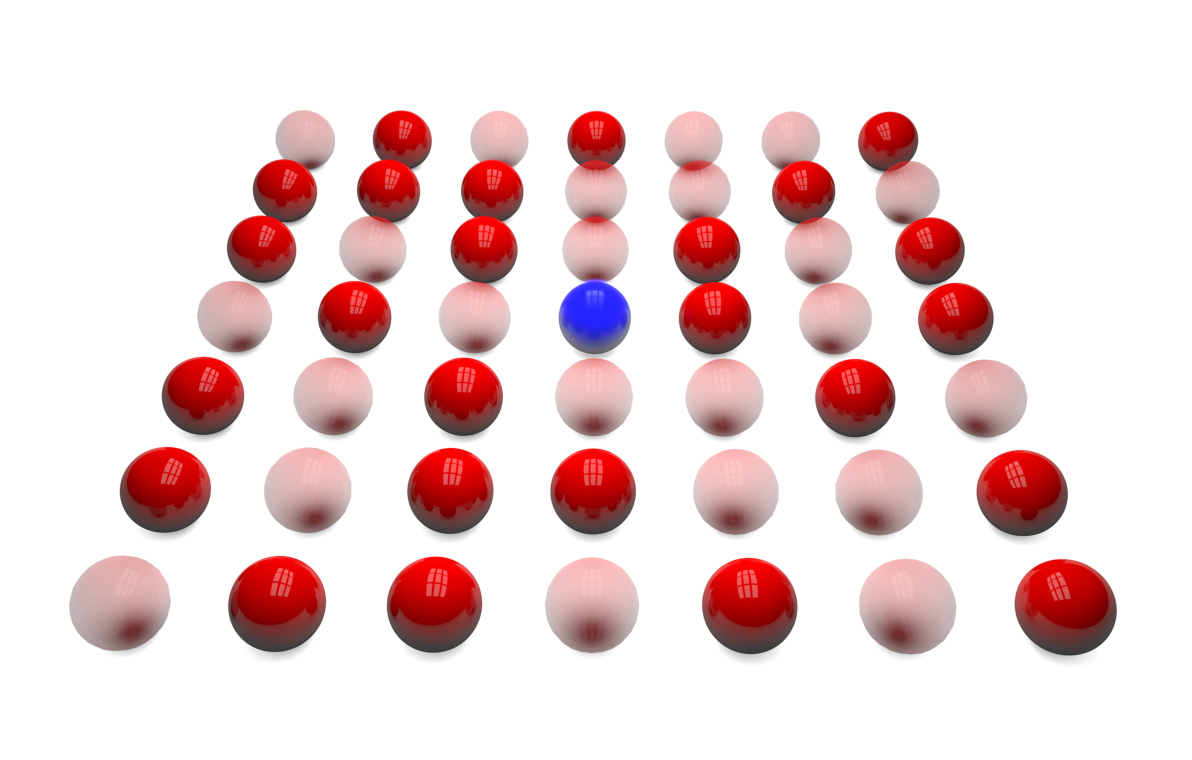
\includegraphics[width=10cm]{chapter_6/figures/fig_1} 
\par\end{centering}
\caption{Schematic representation of a crystalline structure with an edge ($D$)
of 7 particles. The transparent spheres represent the removed particles. The dipole emitter is represented by the blue sphere
and the scatterers by red spheres.\label{fig:crystalline_structure}}
\end{figure}

The structures are generated from the following idea:\\
We start by consider a square lattice with $D \times D$ sites, each site with a set of four adjacent sites. For each lattice site with coordinates $i,j$, there is a discrete variable $\sigma_{i,j}$ such that $\sigma_{i,j} \in \left\{-1,1\right\}$, representing the site spin. So, a system configuration, in this context, is an assignment of a spin value to each lattice site. For any two adjacent sites, $\sigma_{i,j}$ and $\sigma_{\left(i+\zeta\right),\left(j+\zeta\right)}$ with $\zeta = \left\{-1,1\right\}$, there is an interaction $J_{\left[{i,j}\right]\left[{\left(i+\zeta\right),\left(j+\zeta\right)}\right]}$ that allow us to calculate the energy associated to the spin, given by the Hamiltonian:

\begin{equation}
H\left(\sigma_{i,j}\right) = -J_{\left[i,j\right]\left[i,j+1\right]}\sigma_{i,j}\sigma_{i,j+1} - J_{\left[i,j\right]\left[i,j-1\right]}\sigma_{i,j}\sigma_{i,j-1} - \atop -J_{\left[i,j\right]\left[i+1,j\right]}\sigma_{i,j}\sigma_{i+1,j} -J_{\left[i,j\right]\left[i-1,j\right]}\sigma_{i,j}\sigma_{i-1,j}.
\end{equation}
Initially, we generate a random structure, a square lattice where a random spin is assigned for each site. We assume that the interaction between spins is $J_{\left[{i,j}\right]\left[{\left(i+\zeta\right),\left(j+\zeta\right)}\right]}=1$. \\
For each site, we calculate the difference between energies when the spin $\sigma_{i,j}$ assumes the value of $1$ and $-1$, $\delta E = H\left(-\sigma_{i,j}\right)-H\left(\sigma_{i,j}\right)$. 
So, considering the Metropolis algorithm, the system changes its configuration (from $\sigma_{i,j}$ to $-\sigma_{i,j}$) with a probability $p = e^{-\delta E/\theta}$, with $\theta$ the temperature of the system. \\
If $\delta E < 0$, the probability is $p = 1$ and the new spin configuration is accepted. If $\delta E > 0$ the probability of acceptance the new spin is smaller than $1$. We generate a random number between the interval $\left[0,1\right]$ and we compare with $p$. If the random number is larger than $p$, the new spin configuration is refused, otherwise is accepted.\\
This process is repeated to all spin positions a large number of times to obtain independent configurations, \textit{i.e.}, that two consecutive configurations be uncorrelated. For the optical calculation, we only consider configurations where the amount of spins $1$ is between $45\%$ and $55\%$. In this work, for each temperature and lattice dimensions, we generate $10^6$ different configurations to perform optical calculations. As already said, the spins with $s=1$ are taken as the locations of the scattering dipoles, while spins with $s = -1$ are considered as dipole vacancies.
%In order to be able to compare both cases we only consider systems with a concentration in the range between $c=0.45$ and $c=0.55$.
The construction of these thermally disordered systems has been largely explored by Marqu�s \textit{et al.} \cite{Marques,MarquesII}.

In these systems, the correlation function between point dipoles separated by a distance $r$  is  given by the spin-spin correlation function \cite{Yeomans}:

\begin{equation}
g(r)\sim r^{-\tau}exp^{-r/\xi}
\end{equation}
with $\xi$ being the correlation length and $\tau$ a characteristic number depending on the system. The correlation length, near the critical temperature of the Ising model ($T_ {c}$), depends on the ordering temperature with a power law given by $\xi\sim(\theta-T_{c})^{-\nu}$, where $\nu=1$ and $T_{c}=2/ln(1+\sqrt{2})$ for the two-dimensional Ising system.\\
Hence, if a high ordering temperature ($\theta\gg T_{c}$) is used to generate a particular realisation, the correlation function of the equilibrium thermal disposition of the dipoles is going to be given by $g(r)\sim exp(-r/\xi)$, {\it i.e.}, we have a random (short-range correlated) disorder similar to the one used in previous investigations \cite{Froufe_2008, Martorell_1991,Sapienza_2011}. However, if $\theta$ happens to coincide with the characteristic critical temperature of the pure Ising model ($\theta=T_{c}$) then $\xi \rightarrow \infty$ and we are going to have scatterers randomly located, but following a long-range correlated distribution given by $g(r) \sim r^{-\tau}$.  The dispersion on dipole concentration ($c$) obtained by a thermal distribution at $\theta=T_{c}$ is larger than the one obtained when scatterers are randomly distributed with no correlation.

We consider a square lattice with lateral size $D$, where the emitter is placed in the central position of the lattice and oriented out of plane (see Fig. (\ref{fig:crystalline_structure})). 

We consider a particular frequency ($\omega = \omega_{0}$) and an associated particular wavenumber ($k =\omega_{0}/c$) at which dipoles are in resonance with the electromagnetic radiation, meaning that the polarisability is now given by $\alpha = i6\pi/k^3$, like discussed in chapter (\ref{sec:chap2_resonant}). 
In the presence of $\mathcal{N}$ dipole scatterers, the electric field at some point $\mathbf{r}$ is obtained by the superposition principle:

\begin{equation}
{\mathbf{E}\left(\mathbf{r}\right)=\frac{k^{2}}{\epsilon_{0}}\mathbf{G}\left(\mathbf{r},\mathbf{r}_{0}\right)\boldsymbol{\mu}+\atop +\frac{k^{2}}{\epsilon_{0}}\sum_{{m=1}}^{N}{\mathbf{G}\left(\mathbf{r},\mathbf{r}_{m}\right)}\mathbf{p}_{m},}\label{eq:electric_field}
\end{equation}
where $\mathbf{r}_{0}$ is the position of the dipole emitter $\boldsymbol{\mu}$, $\mathbf{r}_{m}$ is the position of scatterer $m$ and $\mathbf{p}_{m}=\epsilon_{0}\alpha\mathbf{E}(\mathbf{r}_{m})$ is the value of the induced dipole located at $\mathbf{r}_{m}$. To obtain the value of all induced dipoles we should solve the electric fields in Eq. (\ref{eq:electric_field}) by considering the coupled dipole method (see chapter (\ref{chap:chap2_DDA})).
The second term on the right-hand side of Eq. (\ref{eq:electric_field})
represents the modification of the free-space dyadic Green function
due to the presence of the scatterers. The scattered field in the dipole emitter position is then given by:

\begin{equation}
\mathbf{E}_{s}\left(\mathbf{r}_{0}\right)=k^{2}\alpha\sum_{{m=1}}^{N}{\mathbf{G}\left(\mathbf{r}_{0},\mathbf{r}_{m}\right)}\mathbf{E}(\mathbf{r}_{m}).\label{eq:scattering_field}
\end{equation}
Once the scattered field is known, the normalized spontaneous decay rate
$\Gamma$ of a dipole $\boldsymbol{\mu}$, in the weak-coupling regime, is given by:

\begin{equation}
\frac{\Gamma}{\Gamma_{0}}=1+\frac{6\pi\epsilon_{0}}{\left|\boldsymbol{\mu}\right|^{2}k^{3}}\Im[\boldsymbol{\mu}^*\cdot\mathbf{E}_{s}\left(\mathbf{r}_{0}\right)],\label{decay_rate}
\end{equation}
where $\Im$ is the imaginary part and $\Gamma_{0}$ is the decay rate of the emitter in free space. It is important to take into account that the expression for the spontaneous decay rate we are considering is an approximation valid only for the weak interacting field. In fact, Eq. (\ref{decay_rate}) is obtained by quantum electrodynamics calculations of the spontaneous decay rate of an atomic system in an inhomogenous medium when the weak-coupling regime approximation is considered \cite{Novotny_PNO_2012}.

\section{Results and discussion \label{chap:chap6_discussion}}

First, we analyse the full crystalline configuration and calculate the normalized decay rate of the emitter, positioned in the center of the structure, as a function of the ratio between the lattice parameter $a$ and the resonance wavelength considered $\lambda=\frac{2\pi}{k}$. We fix the wavelength of the emitter and we vary the lattice parameter.\\
Results presented in Fig. (\ref{fig:crystalline_spectrum}) for a system with lateral dimension $D=23$, allow us to identify a maximum at $\frac{a}{\lambda}=0.44$ with value $\Gamma/\Gamma_{0}\sim7$. 

\begin{figure}[h]
\begin{centering}
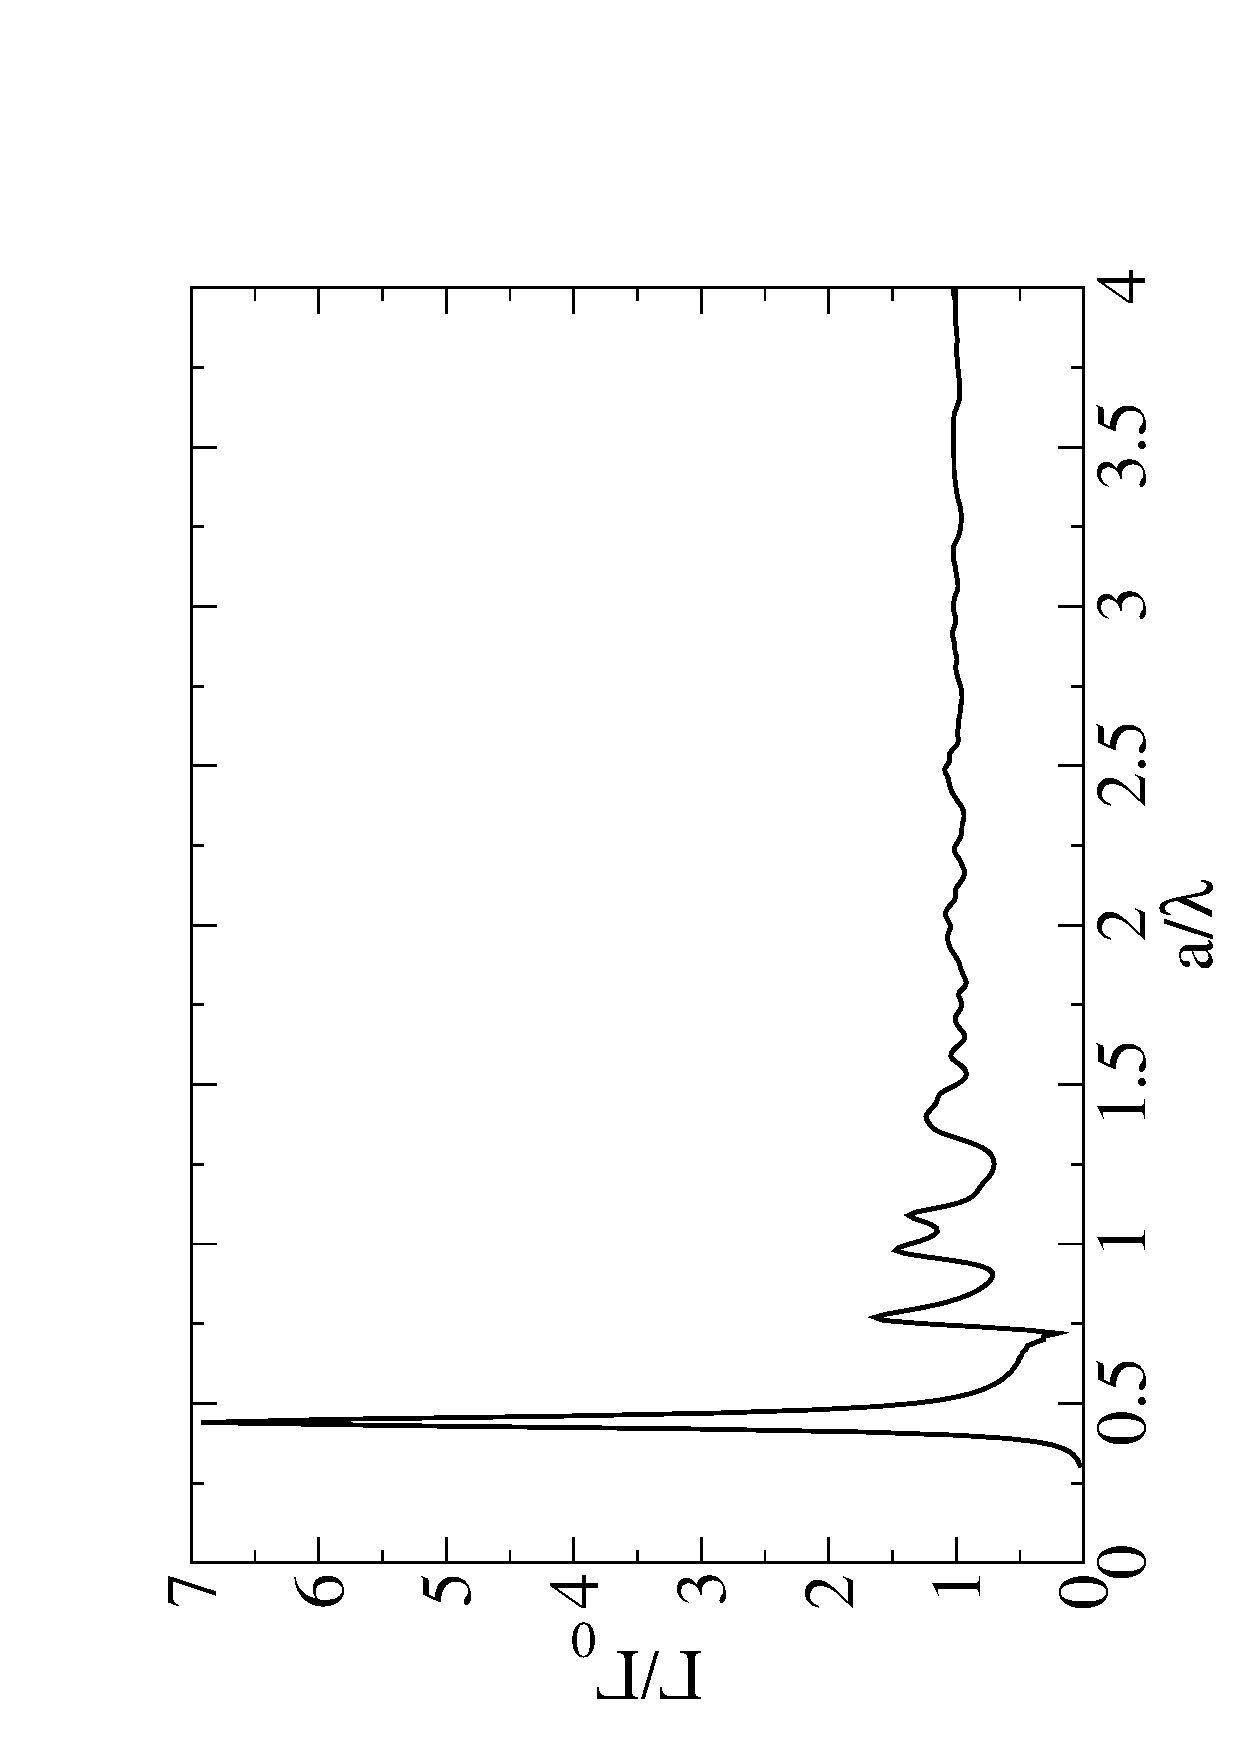
\includegraphics[angle=-90, width=9cm]{chapter_6/figures/fig_2} 
\par\end{centering}
\caption{Normalized decay rate of a crystalline structure for a system with
edge of $23$ particles (total system with $528$ particles). The maximum
can be found at $\frac{a}{\lambda}=0.44$.\label{fig:crystalline_spectrum}}
\end{figure}

Next, we fix the lattice parameter to $a=0.44\lambda$ and we analyse the decay rate distribution for disordered systems generated at different ordering temperatures ranging from $\theta \gg T_{c}$ ($\xi \rightarrow 0$) corresponding to a short-range correlated disorder to $\theta=T_{c}$ ($\xi \rightarrow \infty$), corresponding with a long-range correlated distribution of the vacancies. Results, for $10^{6}$ different configurations, are shown in Fig. (\ref{fig:temperature}).

\begin{figure}[h]
\begin{centering}
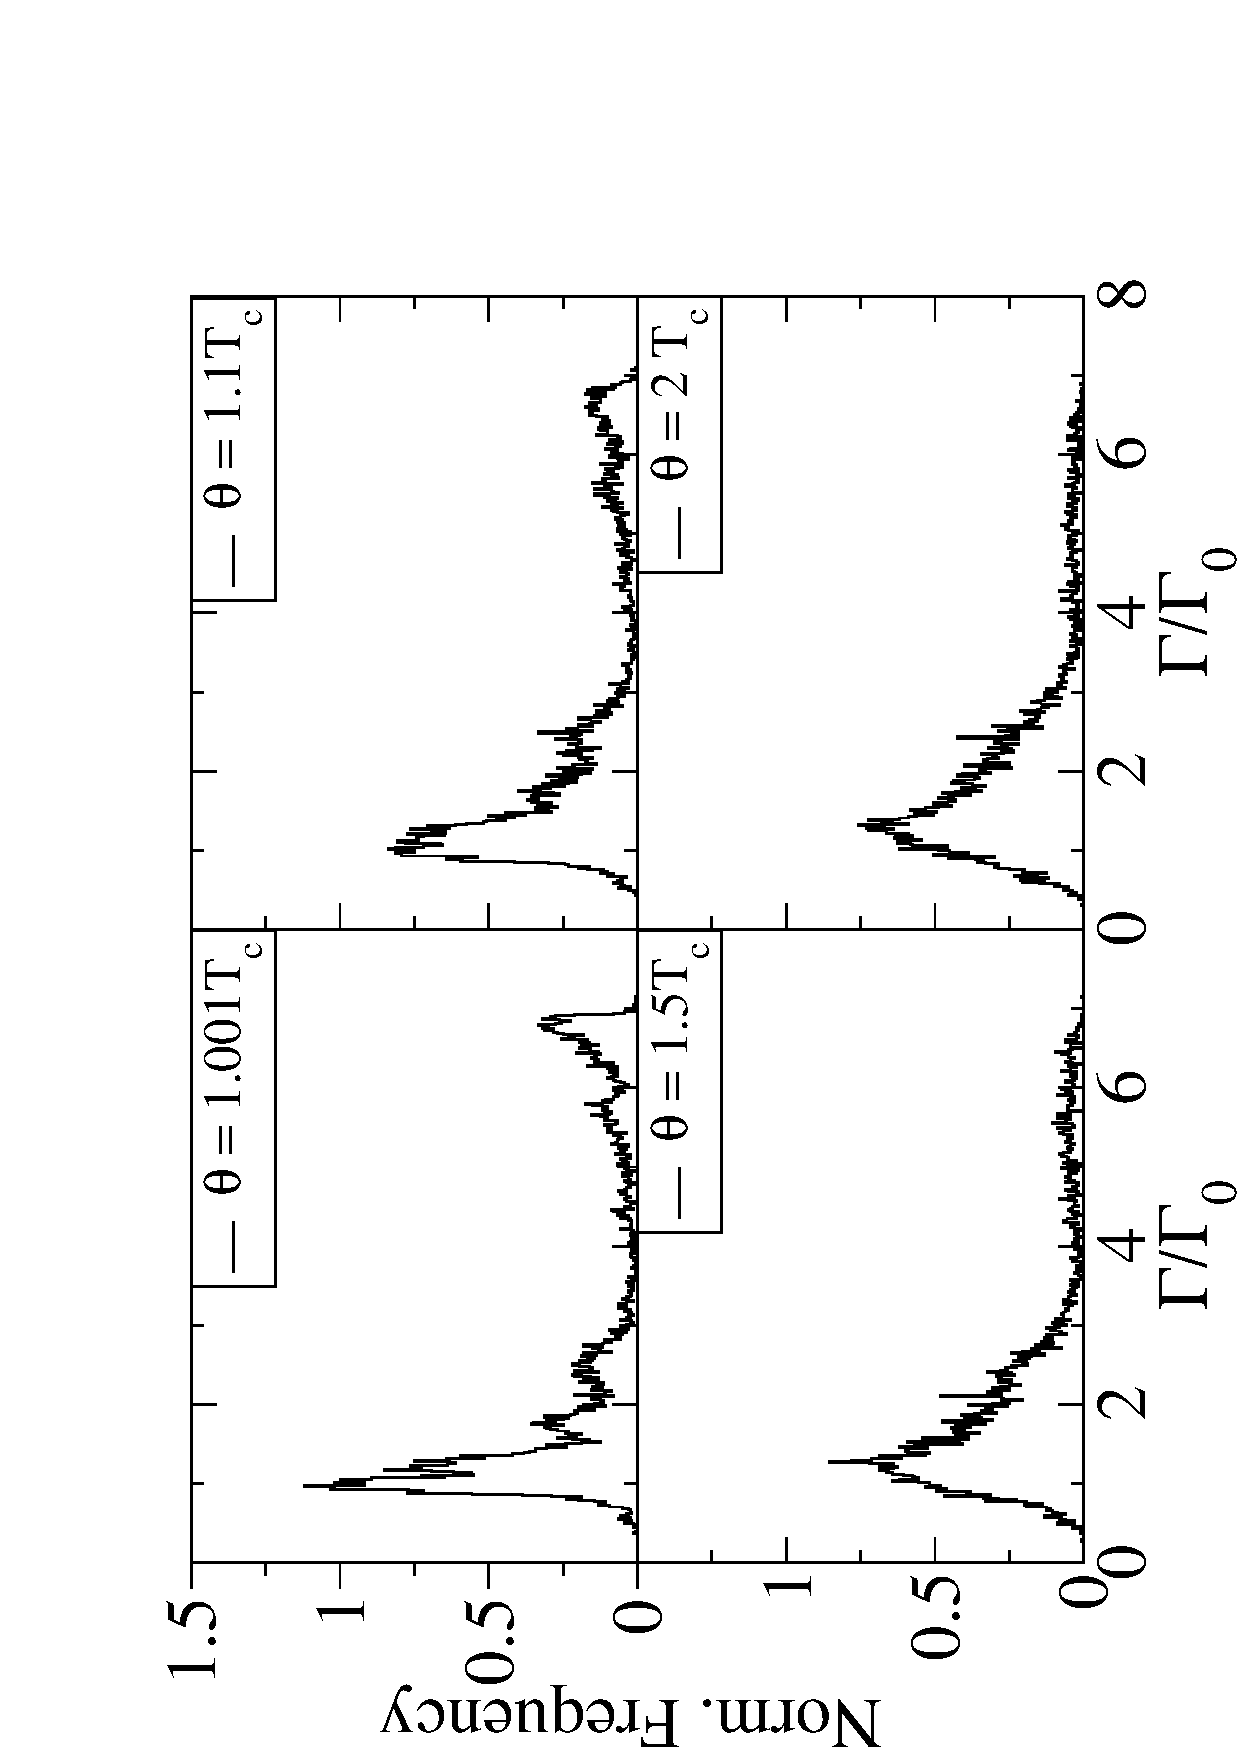
\includegraphics[angle=-90, width=11cm]{chapter_6/figures/fig_3} 
\par\end{centering}
\caption{Normalized histogram of the decay rate for $10^{6}$ different configurations
for a system with $D=23$.
\label{fig:temperature}}
\end{figure}

When the ordering temperature is large ($\theta \sim 2T_{c}$), we obtain a long-tailed distribution centered at $\Gamma/\Gamma_{0} \sim 1.3$, where some rare events are detected for values as high as  $\Gamma/\Gamma_{0} \sim 7$. Similar results have been previously reported \cite{Sapienza_2011, Froufe_2008}. However, as the ordering temperature decreases towards $T_{c}$, the correlation function between vacancies changes from an exponential decay to a power law  and the decay rate distribution reshapes dramatically. For $\theta=1.001T_{c}$, there is  no longer any long-tailed behaviour, but a bimodal distribution where the previously reported rare events increase considerably to build a new maximum centred at $\Gamma/\Gamma_{0} \sim 7$.\\
We have also analysed the possible presence of finite size effects by considering different lateral sizes ranging from $D=13$ to $D=63$ for $\theta=T_{c}$. Results are shown in Fig. (\ref{fig:histogram_all}). Note how all secondary maxima between $\Gamma/\Gamma_{0} \sim 1$ and $\Gamma/\Gamma_{0} \sim 7$ tend to smear out, while maxima at $\Gamma/\Gamma_{0} \sim 1$ and $\Gamma/\Gamma_{0} \sim 7$ are reinforced when the lateral size increases. 

\begin{figure}[h]
\begin{centering}
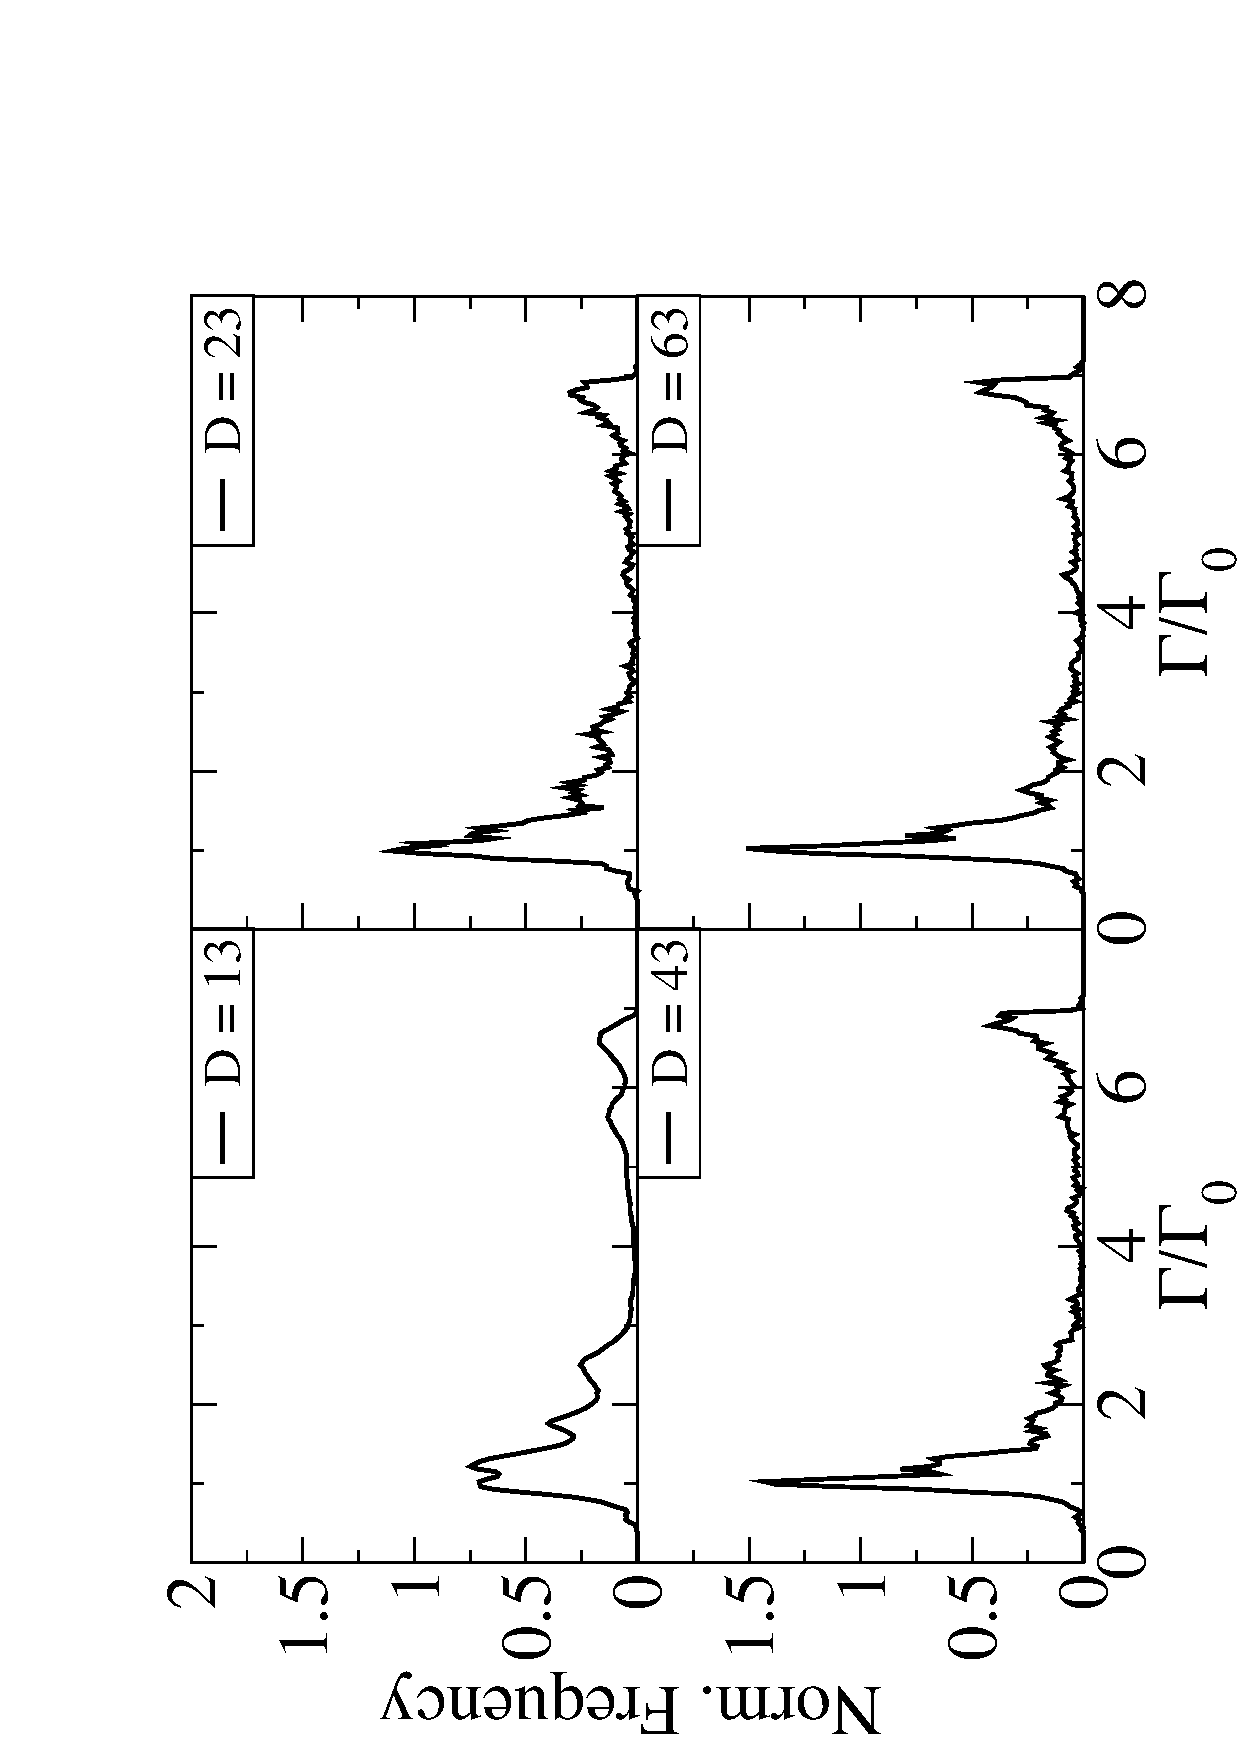
\includegraphics[angle=-90, width=11cm]{chapter_6/figures/fig_4} 
\par\end{centering}
\caption{Normalized histogram of the decay rate for $10^{6}$ different configurations at $\theta = T_{c}$.
The systems under study have an edge of $13$, $23$, $43$ and $63$, with a total of $168$, $528$, $1848$ and $3968$ particles repectively.\label{fig:histogram_all}}
\end{figure}

Large Purcell factors are due to optical modes confined around the source and are sustained by near-field interactions \cite{Sapienza_2011}. So systems with strong correlations, like the ones reported here, should promote an increase in the number of configurations where the emitting dipole is surrounded by clusters of dipoles allowing for field confinement. Due to the correlations, the two most probable configurations around the source are all sites occupied or unoccupied. To further analyse this idea, we plotted the histograms for systems with edge $23$, $43$ and $63$, for different values of the decay rate. The histograms represent the frequency of occupation for each position, normalized to the number of configurations. Black regions represent low occupation, while yellow regions represent sites with large occupation.
% we plotted the histogram of the frequency of occupation for each position normalized to the number of configurations, for different values of the decay rate. 
We focused our attention on $\frac{\Gamma}{\Gamma_{0}}=1.31\pm0.02$, corresponding to the maximum of the distribution for $\theta=2T_{c}$ ,when vacancies in the system are not correlated, and $\frac{\Gamma}{\Gamma_{0}}=0.98\pm0.02, 6.88\pm0.02$ corresponding to the two main maxima of the distribution for $\theta=T_{c}$, when vacancies in the system are correlated. Results are shown in Fig. (\ref{fig:col_hist}).



\begin{figure*}
\begin{centering}
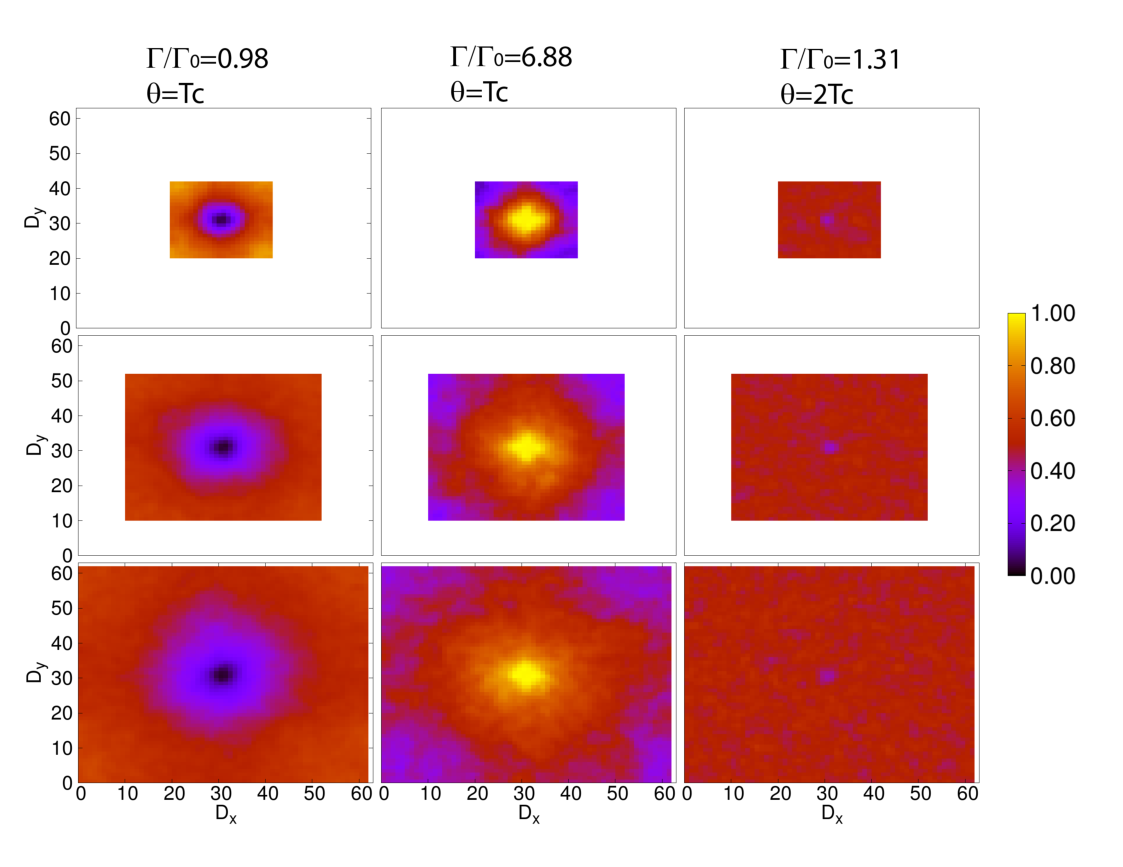
\includegraphics[width=0.8\paperwidth]{chapter_6/figures/fig_5} 
\par\end{centering}

\caption{Colormap histogram of the occupied positions for different size systems
(on vertical: $D=23$, $D=43$, $D=63$). We present three ordering temperatures, two at critical temperature ($T_{c}$), where the system present long range correlations, and one at high temperature ($2T_{c}$), where particles in the system are noncorrelated. Each histogram is normalized by the number of structures corresponding to each decay rate. \label{fig:col_hist}}
\end{figure*}




For $\frac{\Gamma}{\Gamma_{0}}=1.31$ we detect no special patterns, and dipoles are distributed almost randomly. However, for $\frac{\Gamma}{\Gamma_{0}}=6.88$ (corresponding to the second maximum for $\theta=T_{c}$) the dipoles distribution changes markedly. In this case, the emitting particle is clearly surrounded by scattering dipoles, allowing for confinement of the optical modes. This is in agreement with the attribution proposed by Sapienza \textit{et al.} \cite{Sapienza_2011} and clearly shows how large Purcell factors are boosted by long-range correlations in the disordered sample.  Interestingly, for the other maximum located at $\frac{\Gamma}{\Gamma_{0}}=0.98$, the situation is just the opposite and the emitting dipole is, on average, surrounded by vacancies where no field confinement is possible, entailing a dipole response similar to the one found in vacuum. This last effect is also fostered by the existence of long-range correlations when $\theta=T_{c}$. \\
In order to understand these effects, it is important to take into account that, at criticality, clusters of all sizes, containing either dipoles or vacancies,  exist on the system and the response due to larger clusters resembles the one found for the crystalline structure $\frac{\Gamma}{\Gamma_{0}} \sim 7$. However, when a noncorrelated distribution of vacancies is considered, the correlation length and the cluster's sizes are very small, and the detection of events with a large Purcell factor turns out to be very unlikely. The surface structure of the clusters in the Ising model for long-range correlation, \textit{i.e.} at criticality, is known to be fractal and scale invariant \cite{coniglio1989fractal}, like the clusters obtained for high filling factors in semicontinuous metal films experiments \cite{krachmalnicoff2010fluctuations}. These structures are responsible for surface plasmon localisation leading to a large increase in the decay rates. 

\section{Conclusion \label{chap:chap6_conclusions}}

In conclusion, the normalized fluorescent decay rate distribution has been analysed in a thermally disordered two-dimensional diluted dipole lattice where the correlation between vacancies may be tuned at will. When the ordering temperature is far from criticality, the correlation length is small, and the decay rate distribution shows the typical long-tailed shape where events with large Purcell factors are extremely rare. However, when the ordering temperature is close to criticality, the correlation length tends to infinity, turning the decay rate function into a bimodal distribution where large Purcell factor events are much more probable.\\
Thus, we have demonstrated the dramatic effect of correlations on the emission dynamics statistics. We have shown that, at constant density, the decay rate statistics can vary from mono-modal to bimodal distributions as the correlations increase.
%Our analysis shows that when vacancies are distributed with long-range correlations, enclose clusters of dipoles of all sizes, allowing for the existence of many configurations with optical modes confined around the source. 
 It is worth mentioning the analogy between our model system and related models in the field of optical lattices filled with cold atoms \cite{bloch2008many, bloch2012quantum, froufe2009threshold}, in particular for sparsely filled lattices. This analogy could open another way to study spatial correlations effects on the statistics of fluorescence lifetime.
                                   %Chapter 6
\chapter{Self-diffusion and structural properties of confined fluids in dynamic coexistence\label{chap7}}

\section{Introduction}

The thermodynamics and molecular dynamics of gases, liquids, and solids confined to small volumes can differ significantly from those of the bulk \cite{Pawlow:1909,Hill:1963}. The confinement of a fluid in a region few times the particle diameter induces density layering and solvation force oscillations \cite{Hansen:2006,Israelachvili:1991,bhushan1995nanotribology} and can strongly modify the dynamical properties of the fluid \cite{Granick1991,Klein1995,Wales1996}, such as the diffusion of its constituents \cite{Erpenbeck:1991,Thompson1992,Gao1997,Mittal:2008,Matsubara:2012}. The confinement also affects many other macroscopic properties of the fluid \cite{Gelb:1999}, from capillary condensation \cite{evans1984theory,kober2010nanogeometry} to melting/freezing phase transitions \cite{briant1975molecular,Buffat:1976,berry1984melting,Honeycutt:1987,berry1988solid,ercolessi1991melting,schmidt1998irregular,Baletto2005}.\\
For most liquids, the self-diffusion coefficient in highly confined geometries can decrease (the viscosity can increase) by several orders of magnitude with respect to the macroscopic bulk values \cite{Granick1991,Klein1995,Erpenbeck:1991,Thompson1992,Gao1997,Mittal:2008,Matsubara:2012}. Although confinement strongly affects local structuring, the relationship between self-diffusivity and thermodynamic quantities were found to be, to an excellent approximation, independent of the confinement \cite{Mittal:2008,Mittal:2006}, suggesting that thermodynamics can be used to predict how confinement impacts dynamics \cite{Rosenfeld:1977}. More recently, it has been shown that dynamic and equilibrium properties have been explicitly related in supercooled and strongly confined liquids \cite{ingebrigtsen2013predicting}. These findings open an interesting question about the nature of the self-diffusion near the freezing/melting transition in confined geometries. In contrast with macroscopic systems, for small clusters the transition does not take place at a well defined temperature: there is a finite temperature range where solid and liquid phases may coexist dynamically in time \cite{briant1975molecular,berry1984melting,Honeycutt:1987,berry1988solid,Labastie1990,Wales1994,Cleveland1994,schebarchov2005static}, {\it i.e.}, observing the cluster over a long time, the cluster fluctuates between being entirely solid or liquid.\\ 
Numerical simulations have been extensively used to analyse the size dependence of the thermodynamic properties of confined fluids and clusters \cite{briant1975molecular,Honeycutt:1987,berry1988solid,Quirke:1988,Polak:2006}. Concerning the dynamics and size-dependence of self-diffusion in confined fluids, most of the theoretical work have been focused on numerical Molecular Dynamics (MD) simulations \cite{Beck1990,Erpenbeck:1991,Yeh:2004,Thompson1992,Gao1997,Mittal:2008,Matsubara:2012}. Dynamic coexistence is not always observed in simulations \cite{Cleveland:1999} because it depends on the time scale on which dynamic coexistence occurs \cite{schebarchov2005static}, which can be very large depending on the magnitude of the energy barrier separating the solid and liquid states of the cluster. Dynamic Monte Carlo (DMC) simulations \cite{Binder1994} offer an alternative approach that can be used to describe self-diffusion at large time scales \cite{Huitema:1999} where both MD and DMC simulations reveals self-diffusion in confined fluids as a thermal activated process \cite{Matsubara:2012}. \\
%The experimental measurement of the dynamic properties of confined systems in small volumes has proven to be a difficult talk. A possibility, is the study of the optical properties in such systems and relate them with the thermodynamic properties.
% Here we present a study of the thermodynamical properties of a confined fluid. In chapter (\ref{chap8}) we relate the thermodynamical properties with optical calculations.

In this chapter we analyse and discuss the peculiar behaviour of the self-diffusion coefficients and radial distribution function (also called pair correlation function), $g\left (r\right )$, in a confined Lennard-Jones in the solid-liquid dynamic coexistence region. We should stress that in this confined systems the structure and dynamical properties are not homogeneously distributed though the system, being the properties of the surface particles different from the bulk. As a consequence, the spatial average of relevant quantities  could hide or even give rise to wrong physical interpretation. This is the case of the (time and spatial) averaged structure factors as we will see are essentially indistinguishable among both phases. However, as we will show, the average of the self-diffusion coefficients vary largely from liquid to solid phase, thus providing an unambiguous signature of the actual phase.
Surprisingly, we find that the $g\left (r\right )$ is essentially indistinguishable among both phases, while the self-diffusion coefficients vary largely from liquid to solid phase.\\
More specifically, we study the self-diffusion coefficient of a medium size ($515$ atoms) Lennard-Jones (L-J) cluster confined in a spherical cavity as a function of the temperature. In the liquid (fluid-like) phase, just above the melting temperature, the self-diffusion coefficient obtained from DMC numerical simulations follows the typical Arrhenius behaviour expected for thermal activated diffusion. 
In the coexistence region, the self-diffusion randomly jumps between liquid-like to solid-like reinforcing the relationship between dynamic and thermodynamic properties even in this region. Although the confinement induces a strong anisotropy of the pair correlation functions of the fluid \cite{Nygard2012}, we find no significant differences in the average radial distribution function between the two phases. Our results suggest that the direct observation of dynamic coexistence could be accessible by experimental approaches sensitive to self-diffusion by Nuclear Magnetic Resonance \cite{kimmich1997nmr} or Fluorescence Correlation Spectroscopy \cite{magde1974fluorescence} measurements for instance. As we shall discuss in chapter (\ref{chap8}), lifetime statistics is a strong candidate to identify differences in the dynamic properties.\\
In Sec. (\ref{chap:chap7_statement}) we describe the physical system and introduce the model under consideration. Sec. (\ref{chap:chap7_discussion}) is devoted to the presentation of the numerical results and discussion. In Sec. (\ref{chap:chap7_conclusions}) we present the central conclusions of this work.

\section{Statement of the model\label{chap:chap7_statement}}

Let us consider a canonical ensemble of point particles interacting through a L-J potential:

\begin{equation}
V_{LJ}\left(r\right)=4\varepsilon\left[\left(\frac{\sigma}{r}\right)^{12}-\left(\frac{\sigma}{r}\right)^{6}\right],\label{eq:sSH_eq}
\end{equation}
where $\varepsilon$ is the depth of the potential well, $r$ is the distance between particles and $\sigma$ is the distance at which the inter-particle potential is zero.\\
The particles that form the L-J fluid are confined inside a sphere. In order to consider the highest possible density in the system, the radius of the confining sphere is chosen in such a way that a highly symmetric portion of a face centred cubic (FCC) lattice fits the spherical volume. To have nearly relaxed structures at zero temperature, the nearest neighbours distance of the FCC lattice is chosen to be $r_{m}=2^{\frac{1}{6}}\sigma$.

\begin{figure}[h]
\begin{centering}
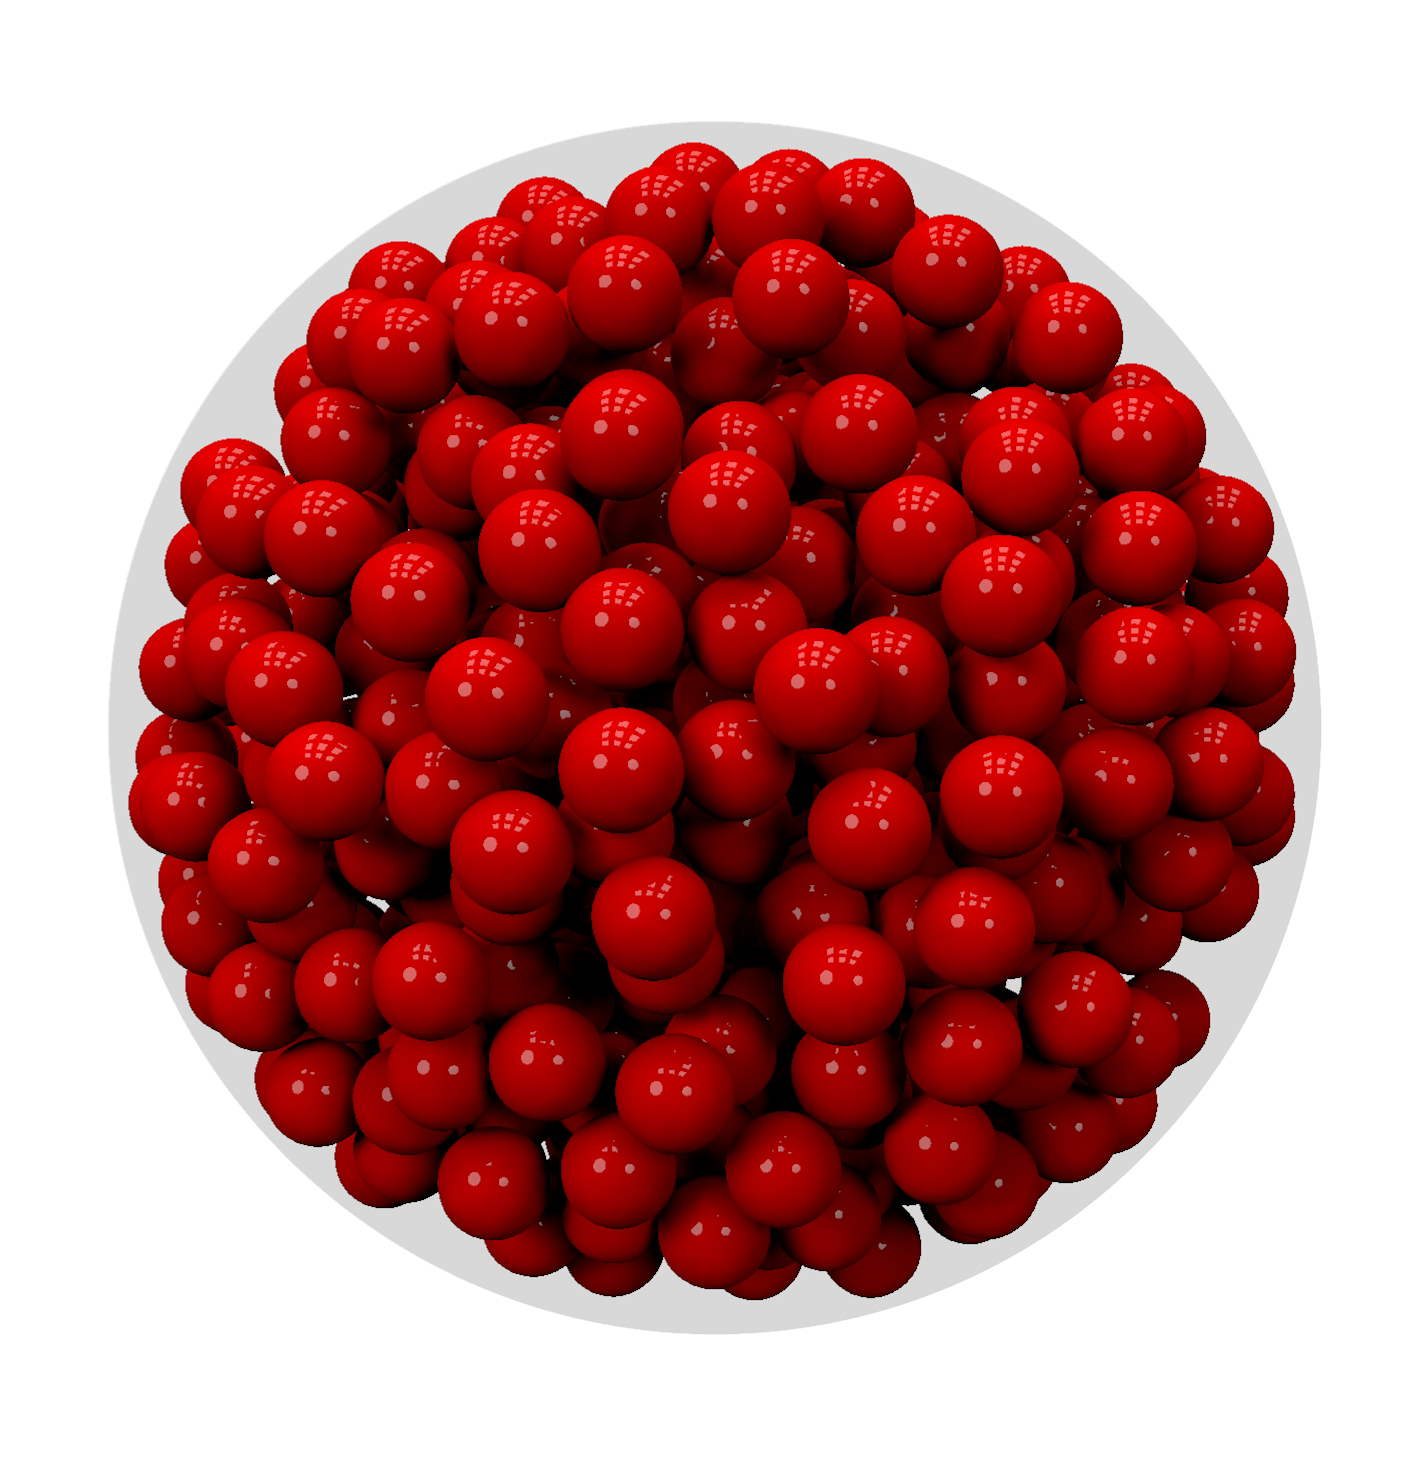
\includegraphics[width=6cm]{chapter_7/figures/fig_1.png} 
\par\end{centering}
\caption{\label{fig:sketch}Representation of the system under study. The centres of the red spheres represent the particles position. The radius of each sphere equals half the L-J potential equilibrium distance $r_{m}/2$. The translucid sphere represents the confining sphere.}
\end{figure}
Here, unless otherwise specified, we consider $515$ particles as can be seen in the sketch of Fig. (\ref{fig:sketch}). In this figure, the particles are represented by a spheres of radius $r_{m}/2$, and the translucid sphere represents the confining spherical volume. In an infinite FCC lattice the maximum filling fraction is $\phi_{\infty}\simeq74\%$. In the case studied, we reach $\phi\approx56\%$. In the process of the generation of the structure, we imposed a condition that only particles inside of the sphere are considered (note that the particles are point particles). This condition gives rise to a reduction of the maximum filling fraction because inaccessible spaces appear along the confining geometry.\\
In order to generate a suitable statistical ensemble at fixed temperature, we perform DMC simulations using the canonical ensemble. We depart from a relaxed structure with energy $E_{i}$. A particle of the ensemble is randomly chosen and it is moved to a new position. This new position, randomly selected, is inside of a sphere with radius $\tilde{r}$ and centred in the previous position of the particle. If the new position is inside the confining sphere,
%and is not a position already occupied by other particle, 
the new position is a valid position to be considered. Otherwise the particle is replaced in the previous position and the calculation returns to the beginning.  At this point, we re-evaluate the system's energy $E_{f}$. The system changes its configuration from one energy to the other with probability $p = e^{-\frac{E_{f}-E_{i}}{T}}$, where $T$ is a control parameter analog to the temperature.\\
If $E_{f} < E_{i}$, the probability is $p = 1$ and the new position is accepted. A direct consequence is the decrease of the total energy of the system. If $E_{f} \geq E_{i}$ the probability of acceptance the new position is smaller than $1$. We generate a random number between the interval $\left[0,1\right]$ and we compare with $p$. If the random number is bigger than $p$, the position is refused, otherwise is accepted. We should note that the "acceptance rate" is controlled by the temperature parameter $T$.\\
 If the new position is accepted, $\tilde{r}$ is resized by a factor of $1.01$, otherwise $\tilde{r}$ is resized by a factor of $0.99$. The full set of steps described above is called single-particle MC step.
We start by performing $10^{8}$ of MC steps to thermalise the system, where no information is collected.
After this process an extensive MC sampling is performed ($10^{5}$ configurations, each configuration obtained after $10^{5}$ single-particle MC steps), where structural information is collected and treated.\\
Here the temperatures and energies presented are given in units of the potential well.

\section{Results and discussion\label{chap:chap7_discussion}}

We determine the temperatures of the (isochore) phase transition in the system by considering the specific heat (SH). The SH, or $C_{v}$, is obtained through the fluctuations of the internal energy \cite{Wang:2001jk}:

\begin{equation}
C_{v}\left(T\right)=\frac{\partial U\left(T\right)}{\partial T}=\frac{\left\langle E^{2}\right\rangle -\left\langle E\right\rangle ^{2}}{T^{2}}.
\end{equation}

\begin{figure}[h]
\begin{centering}
\includegraphics[height=11cm,angle=-90]{chapter_7/figures/fig_2.eps} 
\par\end{centering}
\caption{\label{fig:specific_heat}(a) Specific heat as a function of temperature for a confined L-J system with $N=515$ particles. Zooms of the specific heat is represent in the box (b) and (c).}
\end{figure}
Considering the behaviour of the specific heat as a function of temperature, as shown in Fig. (\ref{fig:specific_heat})(a), we observe a high and narrow peak for $T\approx0.5$. This behaviour is assigned to a first order phase transition, where the system exhibits a discontinuity in the first derivative of the free energy with respect to the temperature.
Notice that in the phase transition region we have relevant fluctuations, as can be observed in Fig. (\ref{fig:specific_heat})(b). Also we observe a modification on SH for temperatures between $0.4\lesssim T\lesssim0.5$
(Fig. \ref{fig:specific_heat})(c), this feature in the SH might be attributed to a pre-melting region. Out of this transition, the behaviour of the specific heat is continuous. Very similar results were recently obtained by Bolmatov \textit{et al.}, where were presented experimental an theoretical results of the constant-volume SH for noble gases \cite{bolmatov2013thermodynamic}.\\

In order to better describe the phase transitions in the system, we also estimate the self-diffusion coefficient in the system as a function of the temperature. To do so, the averaged quadratic displacement of particles as a function of the performed MC steps were fitted to a linear law. From the slope of the lines, the diffusion coefficient is extracted, as can be seen in Fig. (\ref{fig:quad_disp}).\\

\begin{figure}[h]
\begin{centering}
\includegraphics[height=11cm,angle=-90]{chapter_7/figures/fig_4_1.eps} 
\par\end{centering}
\caption{\label{fig:quad_disp}Quadratic mean displacement as a function of the MC steps for $T=0.45$ and $T=0.55$. The blue and green line are the linear fit used to extract the diffusion coefficient.}
\end{figure}
In Fig. (\ref{fig:diff_coef_1}) we plot the diffusion coefficient ($D$) as a function of temperature for three different systems with different number of particles and different volumes, but obeying to the condition of maximum filling fraction. We observe that the diffusion coefficient, for this scale, does not depend of the size of the system. \\
Three regions can be identified in Fig. (\ref{fig:diff_coef_1}). In the first region, for normalized temperatures $T\lesssim0.4$, the diffusion is strongly inhibited. This fact is compatible with a pure solid phase. The diffusion coefficient grows with temperature at an approximately constant rate in the range $0.4\lesssim T\lesssim0.5$
(See Fig. \ref{fig:diff_coef_1})(b). This apparent increase in $D$ signals a pre-meting phase. It is worth noticing that this region does not correspond to any remarkable feature in the specific heat. The slope of the diffusion constant shows a strong increase at about $T\simeq0.5$, this kink in the diffusion coefficient curve corresponds to the peak in the specific heat.\\
In summary, we can establish a phase landscape in which, we identify a pre-melting region that starts at $T\simeq0.4$, and a (solid-liquid) phase transition at $T\simeq0.5$.

\begin{figure}[h]
\begin{centering}
\includegraphics[height=10cm, angle=-90]{chapter_7/figures/fig_3.eps} 
\par\end{centering}
\caption{(a) Diffusion coefficient as a function of the temperature, for three different system sizes of the system at constant particle density. (b) Zoom of the same plot in the range $0.15<T<0.75$.\label{fig:diff_coef_1}}
\end{figure}
In Fig. (\ref{fig:chap7_energy_fluctuations}) we represent the particle energy as a function of the MC steps for temperature $T=0.53625$, which corresponds to a temperature in the phase transition region. The system at this temperature oscillates between a lower and a higher value of energy. This bistable energy behaviour is the responsible for the fluctuations in the SH. Despite the large number of MC steps used in the sampling, we observe in Fig. (\ref{fig:chap7_energy_fluctuations}) that the number of high and low energy regions is relatively reduced. Hence, if we calculate the SH through the energy fluctuations of internal energy, large fluctuations due to finite sampling is expected, as observed in Fig. (\ref{fig:specific_heat})(b).

\begin{figure}[h!]
\begin{centering}
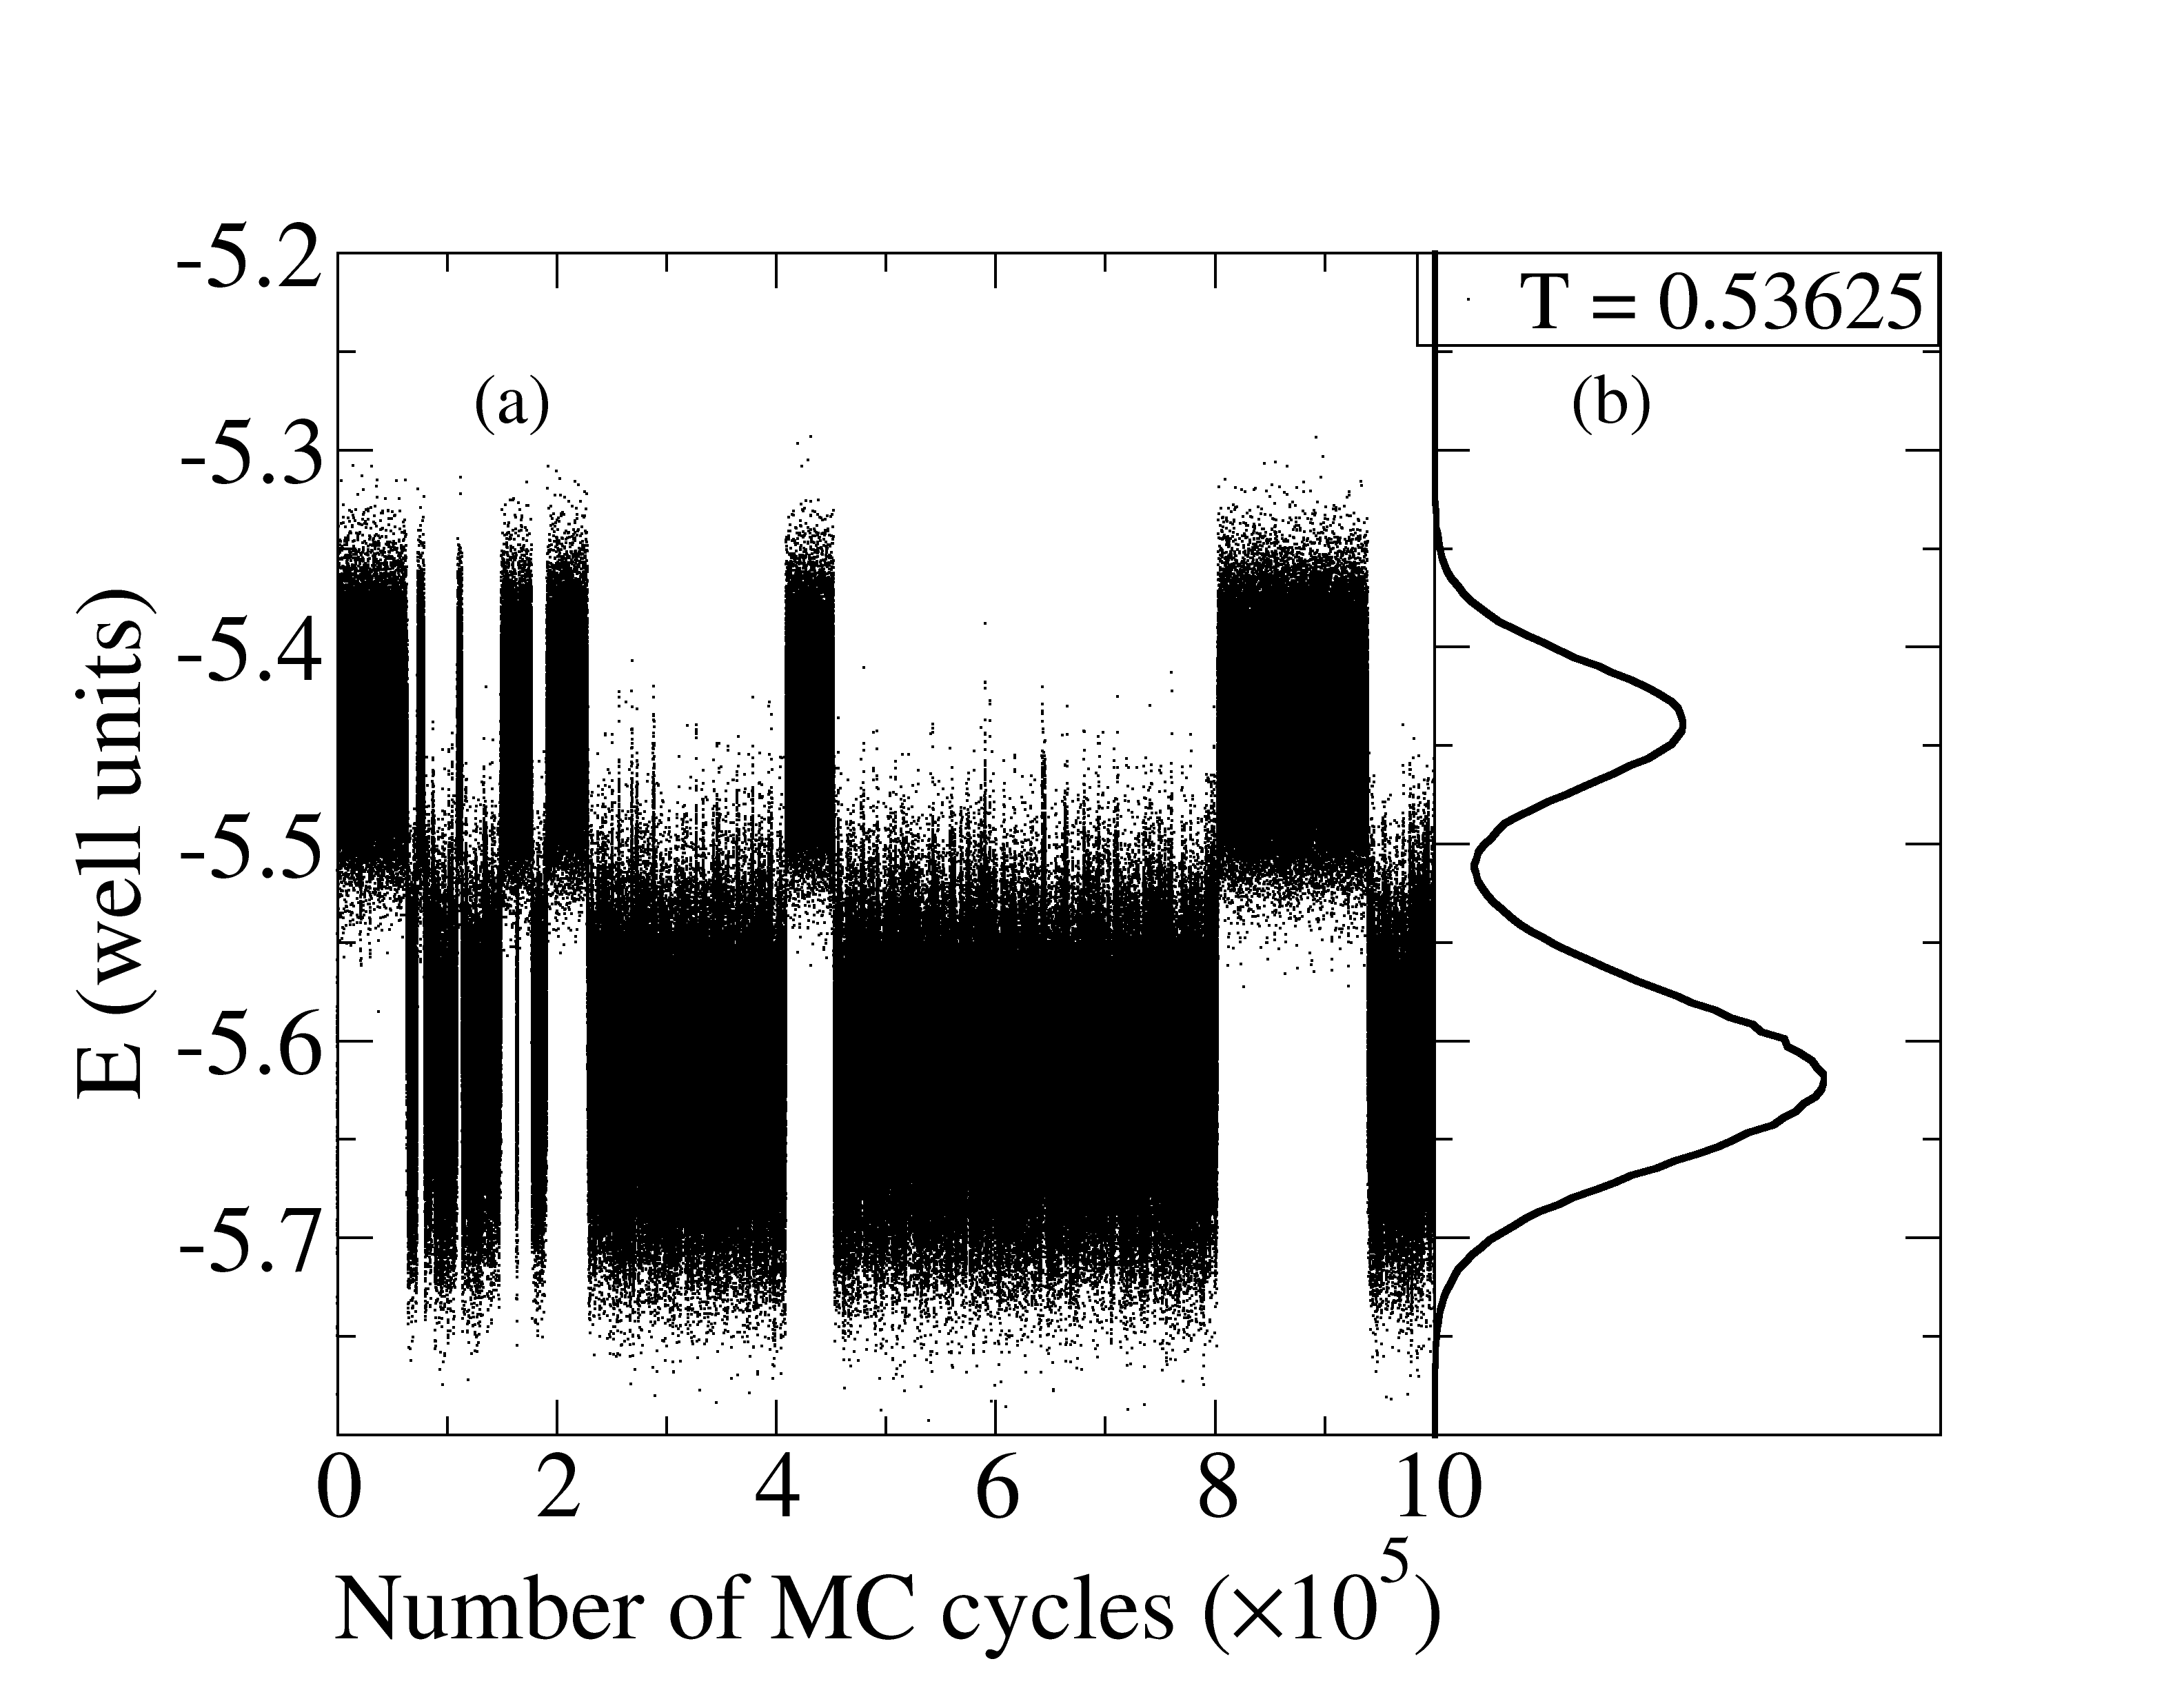
\includegraphics[height=9cm]{chapter_7/figures/fig_4.png}
\par\end{centering}
\caption{\label{fig:chap7_energy_fluctuations} (a) Energy sampling of a confined L-J system during a full MC run at a temperature $T=0.53625$, corresponding to a phase-switching region. (b) Energy histogram obtained from the MC sampling in (a). }
\end{figure}
Representing the internal energy histogram as a function of the temperature, shown in Fig. (\ref{fig:colormap_distrib}), we can identify an energy gap for temperatures at the phase transition. The transition between solid and liquid is not smooth with phase coexistence between two states. Instead, the system switches between this two phases, with abrupt modifications in a small number of MC cycles. In the phase transition, when the particles exhibit a low energy configuration, the system is in the solid phase. For higher energies, the system is in the liquid phase. Interestingly, phase coexistence, that might be attributed to intermediate energies in the energy histogram, appear with very low probability as a gap in the distribution.\\
\begin{figure}[h]
\begin{centering}
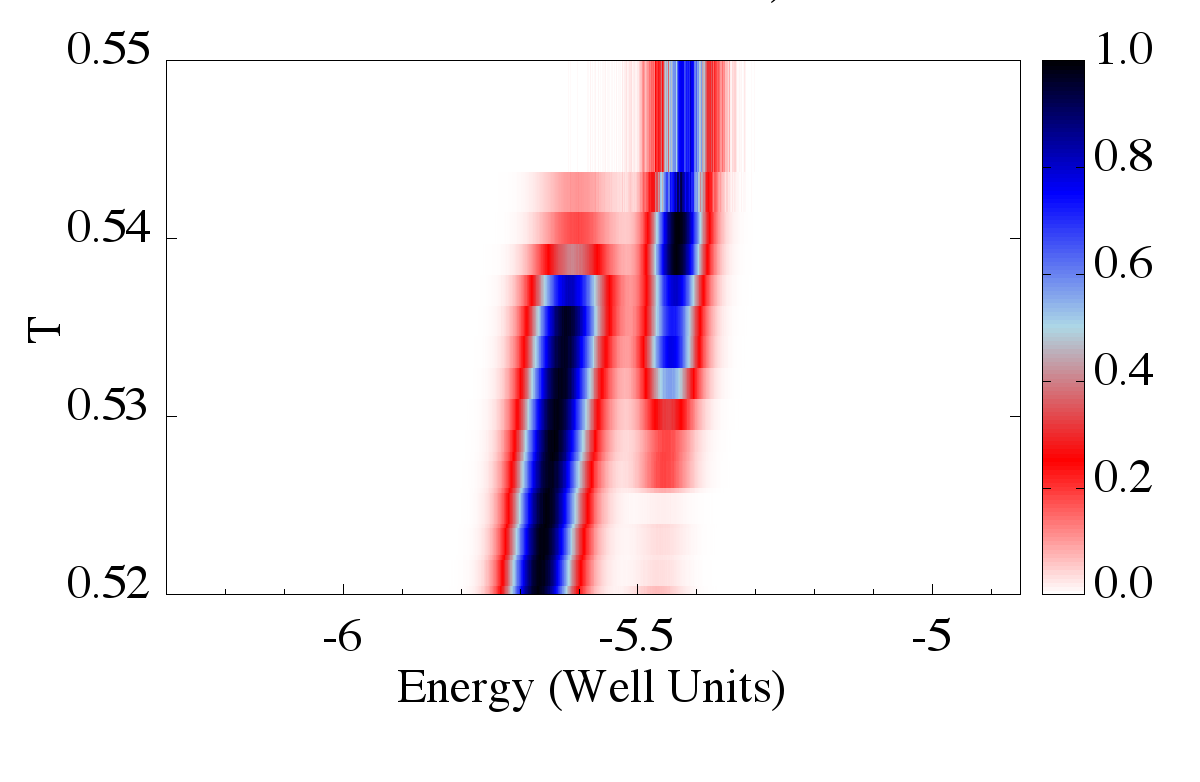
\includegraphics[height=11cm]{chapter_7/figures/fig_5.png} 
\par\end{centering}
\centering{}\caption{(a) Colormap showing the energy distribution functions as a function of the temperature. (b) Zoom in the region corresponding to the solid-liquid phase transition.\label{fig:colormap_distrib}}
\end{figure}
In order to better understand the geometrical and dynamical properties of the system in the phase switching region, we observe that the system remains in either the lower or the upper energy branches for a sufficient amount of time (MC steps) to consider both the structural (pair correlation function) or dynamical (self-diffusion constant) properties in well defined phases.\\
Regarding dynamical properties, in Fig. (\ref{fig:massive_diffusion_coef})(c) we plot the self-diffusion constant as a function of temperature much in the same way as done in Fig. (\ref{fig:diff_coef_1}). In this case, we have split the statistical ensemble in two different sets for temperatures in the phase switching region, one corresponding to the high energy branch (liquid phase), and the other one corresponding to lower energy branch (solid phase). In Fig. (\ref{fig:massive_diffusion_coef})(c) it appears evident that the diffusion coefficients corresponding to both phases can differ by a large amount. In the case under study, the diffusion constant differs by a factor 3 between phases at the same temperature.\\

\begin{figure}[h]
\begin{centering}
\includegraphics[height=10cm, angle=-90]{chapter_7/figures/fig_6.eps} 
\par\end{centering}
\caption{\label{fig:massive_diffusion_coef}(a) Self-diffusion coefficient for a 515 particle system as a function of temperature. (b) Zoom of the self-diffusion coefficient in the range $0.35\leq T\leq0.6$. (c) Self-diffusion coefficients as a function of temperature obtained for the liquid phase (upper branch) and the solid phase (lower branch) in the region of phase-switching.}
\end{figure}
Regarding geometrical properties of both phases in the phase switching region, we have studied the radial distribution function $g\left(r\right)$ \cite{Percus:1958wv,Wertheim:1963tb}. This function is defined as the ratio of the average number density at a distance $r$ from one particle to the averaged number density of an hypothetical, fully uncorrelated, system (see Appendix \ref{App:Radial_distribution_function}). Hence, the radial distribution function describes the correlation in the inter-particle distance in the system. Again, we can split the statistical sampling in two sets associated with upper and lower energy branches in the phase switching region.\\
Contrary to what intuition might suggest, and in contrast with the behaviour of the diffusion constants, the radial distribution function in the upper and lower energy branches is very similar. In Fig. (\ref{fig:chap7_Radial-distribution-function}) we represent the $g\left(r\right)$ for the configurations at both the liquid and solid phase at a fixed temperature.\\
In the solid phase, the structure of the radial distribution function (black line in Fig. (\ref{fig:chap7_Radial-distribution-function})) shows a slightly richer structure than the one corresponding to the liquid phase (red line in Fig. (\ref{fig:chap7_Radial-distribution-function})). Nevertheless, both curves differ by less than 10\% in its values in the whole range of temperatures of the phase switching region, in contrast with the large variations observed in the self-diffusion coefficients. This fact suggests that, despite the subtle peak suppression in $g\left(r\right)$ in the in the switching from solid to liquid phases, a clear identification of different phases through structural measurements (\textit{eg.} radial distribution function) is less sensitive than through dynamical measurements (\textit{eg.} self-diffusion constants) in strongly confined systems. 

\begin{figure}[H]
\begin{centering}
\includegraphics[height=11cm, angle=-90,clip=true]{chapter_7/figures/fig_7.eps} 
\par\end{centering}
\caption{\label{fig:chap7_Radial-distribution-function}Radial distribution function $g\left(r\right)$ obtained at a fixed temperature in the phase switching region ($T=0.53625$) for both the solid (black line) and liquid (red line) phases. }
\end{figure}

\section{Conclusion\label{chap:chap7_conclusions}}

In this chapter we have studied the self-diffusion in a strongly confined Lennard-Jones system. For small clusters, of the order of a few hundreds of particles, instead of phase coexistence, like in macroscopic systems, the system present dynamic phase switching between solid-like and liquid-like phases. This was concluded from monitoring the energy as a function of the system evolution, where the system oscillates between an high energy and a low energy configuration.\\
We found that the self-diffusion coefficient of the liquid-like phase in the phase-switching region can be up to a factor of three larger than the one associated to the solid phase. Surprisingly, the radial distribution function of the liquid and solid phases are essentially indistinguishable. Our results strongly suggest that retrieving relevant information in a system undergoing phase switching involve measurements either of the internal energy evolution or the self-diffusion characteristics of the system. Structural information does not provide a relevant signature of phase switching in this case.\\
In the next chapter we shall study the implications of the behaviour of this system on the optical transport and emission properties.





                                   %Chapter 7
\chapter{Light emission statistics in correlated random photonic nanostructures\label{chap8}}

\section{Introduction}

The statistical properties of light transport and emission in disordered media has been a matter of intense research during the last three decades. Although the basis of coherent multiple scattering is a well known subject, the phenomenon itself have much to explore and its far from be clearly understood \cite{wiersma1997localization}. \\
The interest in disordered systems exhibiting certain structural correlations is due to the fact that these systems can share properties of both crystalline and fully disordered systems. For instance, the conductivity of liquid metals \cite{ashcroft1966structure} or the cornea transparency \cite{hart1969light} can be understood in the same footing: a disordered but correlated system can present spectral regions of high transparency for electron or light transport. Also, strongly correlated charged colloids can scatter light in such a way that the transport mean free path presents a strong chromatic dispersion \cite{Rojas_2004}. Even in the absence of practically any long range correlations, the structure of the scatterers itself can be used to modify the light emission and transport properties of a disordered system in such a way that transport parameters \cite{garcia2007photonic, sapienza2007observation}, or even the threshold of a random laser \cite{gottardo2008resonance}, can present resonances which can be tuned in advance. \\
It is clear that the structure surrounding a single emitter can largely alter its emission dynamics \cite{Purcell_1946,hernando2006effect,desousa2014ising}. In the last years, several groups considered such effects in a statistical way suitable for the description of disordered systems \cite{hernando2006effect,gersen2000influencing, vallee2006fluorescence,Froufe_PRA_2007,desousa2014ising}.  In particular, Vallée \textit{et al.} \cite{vallee2006fluorescence} showed that several structural properties near a phase transition can be accessed via fluorescence intensity fluctuations. It has been theoretically proven that near field scattering in random systems alters fluorescence dynamics in such a way that microscopic information about the surroundings of a single emitter can be obtained from lifetime fluctuations or from the shape of the statistical distribution tails \cite{Froufe_PRA_2007,Froufe_2008,caze2010near,Sapienza_2011}. 

In this chapter we compare light scattering and emission statistics for single emitters embedded in a random scattering medium undergoing a phase transition. In chapter (\ref{chap7}) it was shown that, for a finite and strongly confined system, instead of phase coexistence, the system can present a dynamical phase switching behaviour. Surprisingly, the radial distribution function $g\left(r\right)$ among scatterers in the system is essentially indistinguishable for both phases. Here we show that light scattering measurements performed in the phase-switching regime do not result in differences in the scattering cross section of the system. Nevertheless, calculations of the statistical properties of decay rates of single emitters pinned at the center of the medium can be dramatically different for different phases in the switching regime. Also the lifetime statistics can provide a direct signature of a phase switching behaviour where light scattering measurements are blind to such a dynamical regime.\\
In Sec. (\ref{sec:chap8_statment}) we describe the physical system and introduce the model under consideration. Sec. (\ref{sec:chap8_discussions}) is devoted to the presentation of the numerical results and discussion and in Sec. (\ref{sec:chap8_conclusion}) we present the central conclusions of this work.


\begin{figure}[h]
\begin{centering}
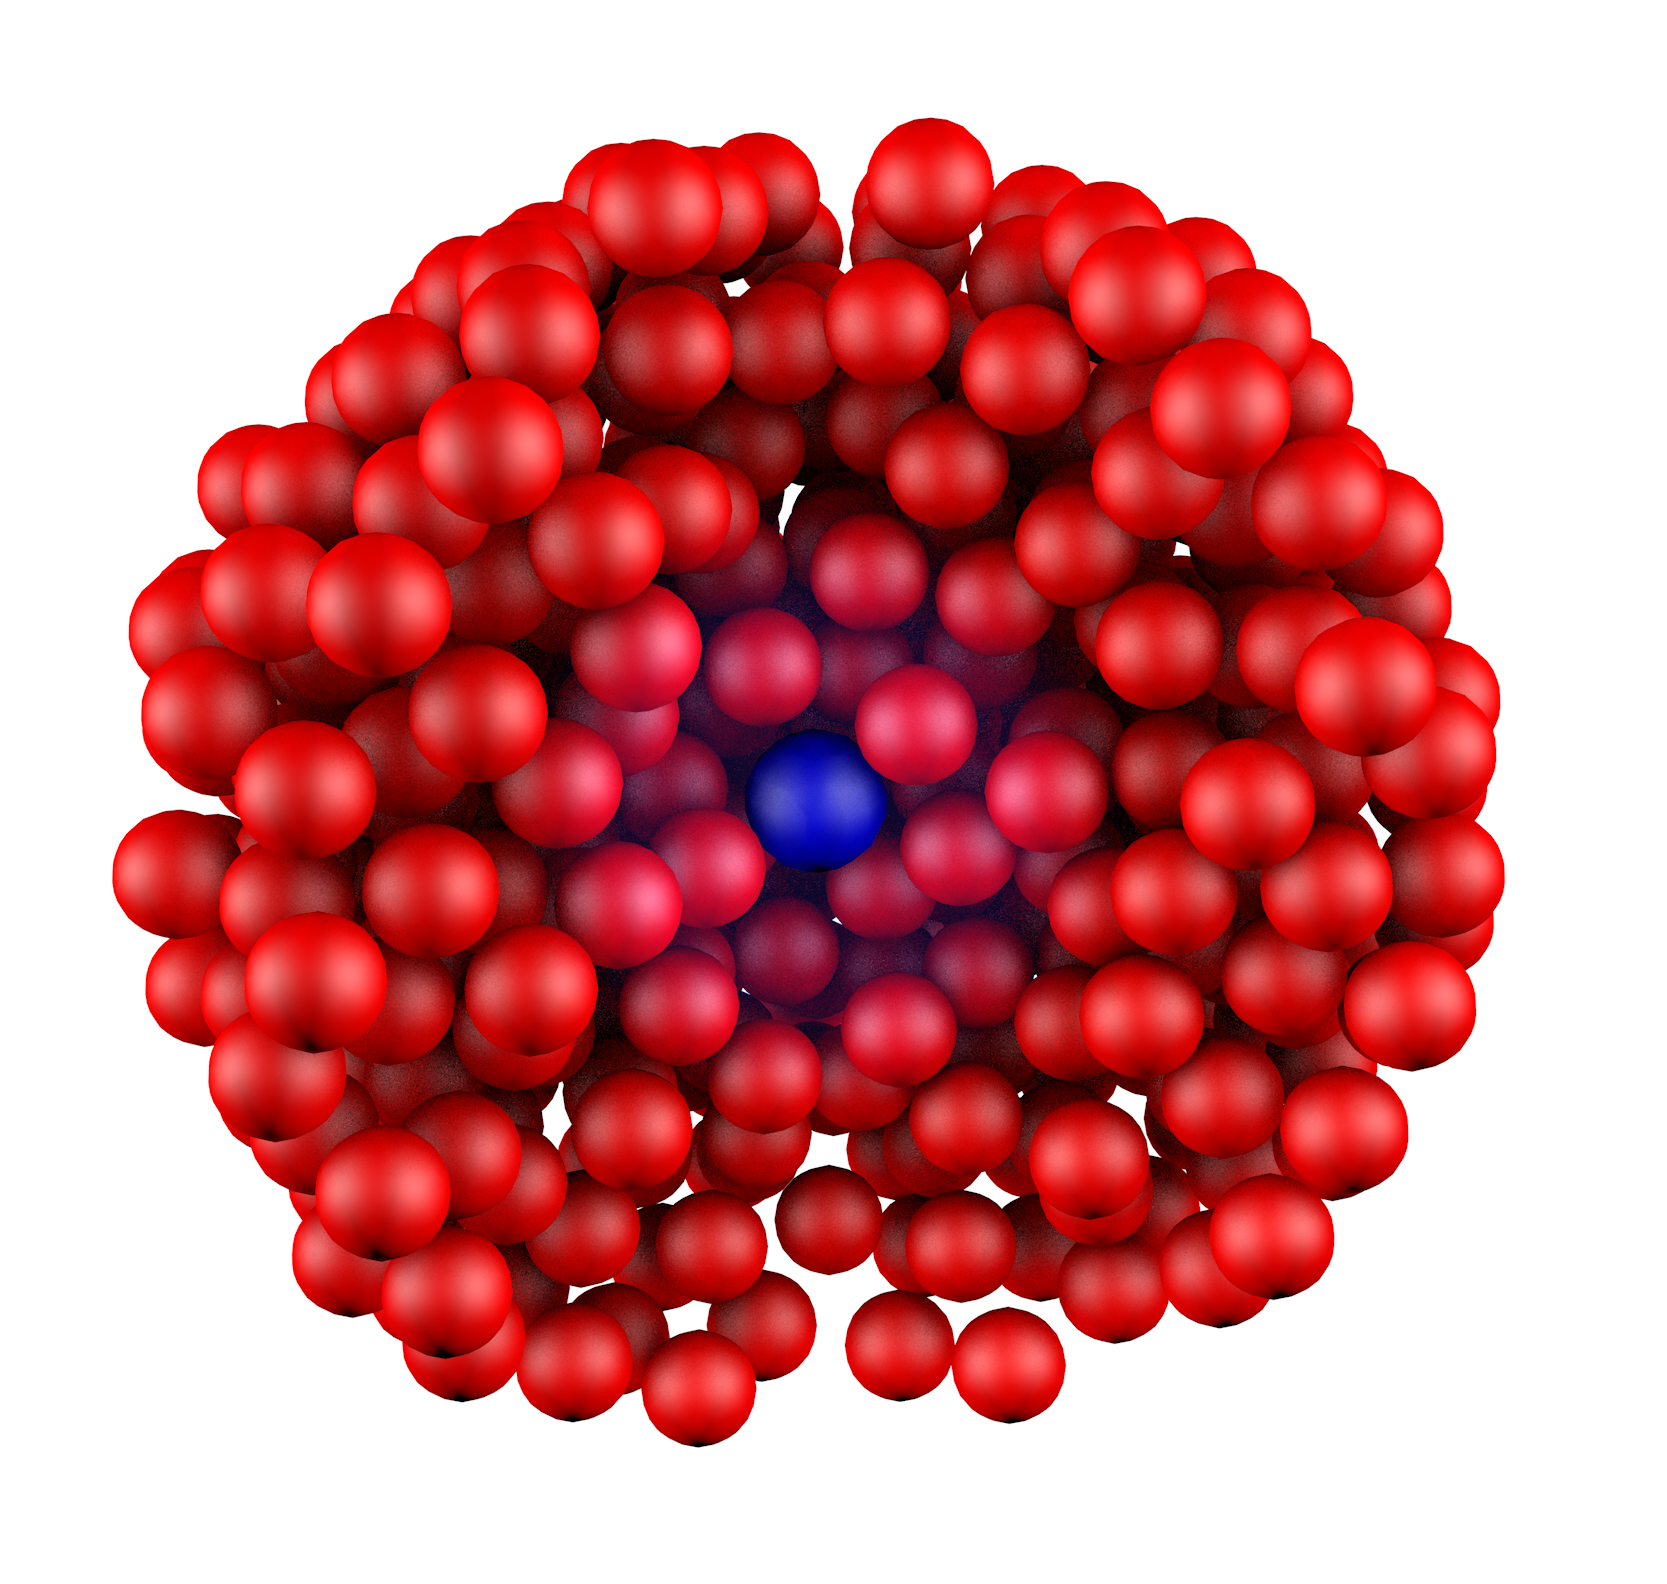
\includegraphics[width=6cm]{chapter_8/figures/sphere_system.png}
\par\end{centering}
\caption{\label{fig:chap8_fig1} Transversal cut of the L-J cluster with $514$ particles. The red spheres represent the point dipole scatterers and the blue sphere in the center represents the point emitter.
}

\end{figure}

\section{Statement of the model\label{sec:chap8_statment}}

The model system under study is a small cluster of $514$ resonant point dipoles interacting through a $\left(12-6\right)$ Lennard-Jones potential. L-J potentials has been extensively studied in the last hundred years. Phase transitions, nucleation dynamics and phase coexistence has been described in great detail in the literature \cite{Hansen:1969tn,Honeycutt:1987,panagiotopoulos1994molecular}.
In chapter (\ref{chap7}) we presented a study of relatively small clusters of particles interacting through L-J potential, in which the systems near a phase transition shows a dynamical phase switching behaviour. In particular, it was demonstrated that in strongly confined clusters with a few hundreds of L-J particles, the system presents an isochoric solid-liquid phase transition at a temperature corresponding to approximately one half of the potential well. Due to the finiteness of the system, the expected specific heat divergence manifests as a peak.\\
In the temperature range corresponding to the phase transition, the system switches in time, in its integrity, between two energetic states that can be associated with solid and liquid phases. In particular, the internal energy clearly shows this behaviour.\\
The pair correlation function obtained in the high and low energy phases is, essentially, indistinguishable. This means that, despite the different dynamical state of each phase, the structural properties of the system, and hence the light scattering properties, should be indistinguishable. We shall consider this point in more detail in following paragraphs.\\
When the self-diffusion coefficients are separately calculated for each phase at constant temperature, we found that there is a three fold variation from solid to liquid phase. Hence, despite the structural indistinguishability among both phases, there is a clear contrast between phases regarding dynamical magnitudes as the internal energy or self-diffusion constants.

The question we want to address is whether or not an optical experiment might show a signature of this phase-switching behaviour.\\
In this chapter we show that indeed this experiment can be realised using fluorescence lifetime statistics measurements but not light scattering.\\
To model the optical response of the interacting particles in the system, we consider each point particle as a point dipole resonant scatterer, similar to those presented in chapter (\ref{chap6}). This model, although not the most general one, covers a wide range of realistic systems that goes from nanoparticles supporting a localised plasmon resonance or cold atom clouds among others. The optical response of the entire system can hence be modelled as an interacting system of point dipoles, a problem that can be readily solved for a system of a few hundred particles in $\sim10^{6}$ different configurations at each temperature by using the coupled dipole method \cite{draine1994discrete}.\\
Using standard Monte Carlo methods, we generate $10^5$ different configurations
of the L-J cluster, each one separated by $10^5$ Monte-Carlo steps. We focus our attention in the temperature of the phase transition, $T\simeq0.53$. We perform light transport and emission calculations for each configuration, evaluating the electromagnetic behaviour of the system as a function of its thermodynamical properties. Results and its subsequent discussion are presented in the next section.

\section{Results and discussion \label{sec:chap8_discussions}}

We start by evaluating the scattering efficiency of a cluster of $515$ L-J particles for different configurations at phase transition temperature. The scattering efficiency is defined by the ratio between the scattering cross section and the geometrical cross section, $Q_{s} = \sigma_{scat}/\sigma_{geom}$.
In Fig. (\ref{fig:fig2}) we present the $Q_s$ (scattering efficiency) sampling at $T \simeq 0.53$. To guide the eye, points corresponding to high and low internal energy are rendered in different colours, where the low energy configuration is rendered in red and the high energy in black. When we integrate the sample in energy, the scattering efficiency histograms are obtained, as shown in Fig.  (\ref{fig:fig2})(a). Differences in $Q_s$ histograms corresponding to high and low energy phases can be hardly distinguished. As expected, we conclude that light scattering experiments would not provide a mean of distinguish among phases in the switching regime.
%We start by evaluating the scattering cross section of a finite crystalline system (FCC lattice) whose first-neighbours distance is the equilibrium distance of the L-J potential $r_{m}$. We obtain a rich pattern in this pseudo-spectrum due to the crystal structure of the system and the resonant character of the scatterers, as can be seen in Fig. (\ref{fig:chap8_crystal_sec}).\\
%
%\begin{figure}[h]
%\begin{centering}
%\includegraphics[width=8cm,angle=-90]{chapter_8/figures/x_sec_vs_k.eps}
%\par\end{centering}
%\caption{\label{fig:chap8_crystal_sec}Scattering cross section spectrum of a crystalline FCC cluster with $515$ L-J particles.}
%\end{figure}
%We take a subset of the whole sam- pling and calculate the scattering cross section of the set of point dipoles. In Fig. 2b ( CREO QUE HAY QUE PRESENTAR LOS PANELES EN ORDEN IN- VERSO: PRIMERO LA NUBE DE PUNTOS Y LUEGO LOS HISTOGRAMAS) we present the energy-Qs (scat- tering efficiency) sampling. To guide the eye, points cor- responding to high and low internal energy are rendered in different colours. Integrating the sampling in energy, we obtain scattering efficiency histograms as shown in Fig. 2a. Differences in Qs histograms corresponding to high and low energy phases can be hardly distinguished. As expected, we conclude the light scattering experiments would not provide a mean of distinguish among phases in the switching regime.
%Nevertheless, not only light scattering in the far field serve as a tool for exploring the structure of a system. Light emission statistics can provide with complementary information.

%We  calculate the energy-$Q_{s}$ (scattering efficiency) for systems at phase transition temperature, $T\simeq 0.53$, with $r_{m}/\lambda = 0.513$, $r_{m}/\lambda=0.466$, $r_{m}/\lambda=0.872$ and $r_{m}/\lambda=0.795$.
%In Fig. (\ref{fig:fig2})(b) we present the results for $r_{m}/\lambda = 0.513$ as example, because for all $r_{m}/\lambda$ the system exhibit a similar behaviour. To guide the eye, points corresponding to high and low internal energy are rendered in different colours. Integrating the sampling in energy, we obtain scattering efficiency histograms as shown in Fig. (\ref{fig:fig2})(a). Differences in $Q_{s}$ histograms corresponding to high and low energy phases can be hardly distinguished. As expected, we conclude the light scattering experiments would not provide a mean of distinguish among phases in the switching regime. \\

\begin{figure}[h]
\begin{centering}
\includegraphics[width=8cm,angle=-90]{chapter_8/figures/2_energy_vs_sec_coex.eps}
\par\end{centering}
\caption{\label{fig:fig2}(a)Energy-scattering efficiency sampling at the switching
region ($T\simeq0.53$, lower panel). (b) We show the
corresponding scattering efficiencies distributions for the upper
energy branch (red distribution) and lower energy branch (black
distribution) corresponding to solid and liquid phases.}
\end{figure}

Nevertheless, not only light scattering in the far field serves as a tool for exploring the structure of a system. Light emission statistics can provide complementary information.\\
In order to assess the possibility of extracting useful information about the structural properties of the system in the switching regime, we consider the statistics of the decay rates of single fluorescent emitters immersed in the structure, as can be seen in the sketch of Fig. (\ref{fig:chap8_fig1}). We start by evaluating the decay rate of a single emitter fixed at the center of the cluster when the particles are perfectly ordered, like in the previous case.\\



%\begin{figure}[h]
%\begin{centering}
%\includegraphics[width=8cm,angle=-90]{chapter_8/figures/3_GratioG0_vs_k.eps}
%\par\end{centering}
%\caption{\label{fig:fig3}Normalized decay rates spectrum of a single emitter
%placed at the center of a FCC cluster.}
%\end{figure}
In Fig. (\ref{fig:figm})(a), we plot the decay rate of a single emitter normalized to its vacuum value as a function of the ratio between the emission wavelength, which is considered to coincide with the scattering resonance of the scatterers, and the inter-particle distance $r_{m}$. As expected, we obtain a rich pattern in this pseudo-spectrum due to the crystal structure of the system and the resonant character of the scatterers. In particular the emission can be enhanced, or even almost completely inhibited. We highlight three representative points in the decay rate pseudo-spectrum: $r_{m}/\lambda=0.466$ and $r_{m}/\lambda=0.872$, where the emission lifetime is shorter than the one in vacuum, and a point at $r_{m}/\lambda=0.795$ where emission is dramatically inhibited. 

%\textcolor{red}{verificar que está feito para estas frequencias Although not shown for the shake of brevity, the scattering efficiency pseudo-spectra are found to be indistinguishable among phases in the switching regime irrespective of the considered value of $r_{m}/\lambda$.}

 
In Fig. (\ref{fig:figm})(b-d), we present an energy-decay rate sampling performed at $T\simeq0.53$ and three different ratios $r_{m}/\lambda$. As can be seen, the energy shows a bimodal distribution, due to the fact that the system is in the phase-switching regime, like represented in Fig. (\ref{fig:chap7_energy_fluctuations}). In analogy with Fig. (\ref{fig:fig2}), samples corresponding to high and low values of the energy are rendered using different colours. Regarding the emitter, we consider the spontaneous emission decay rate of a single emitter placed at the center of the distribution of scatterers. The diffusion of the emitter is much slower than the self-diffusion of scatterers in the system. Hence, a reasonable approximation is to keep the position of the scatterer fixed at the center of the system. The direction of the radiating dipole is random and considered to be uniformly distributed among the whole $4\pi$ angles. In this case, the emitter is placed at the center of a spherical volume excluded to scatterer, where we fix the radius of the real cavity to be $r_{cav}=r_{m}$. This real cavity model \cite{Froufe_PRA_2007,Sapienza_2011} has been extensively used in the literature. 

\begin{figure}[h]
\begin{centering}
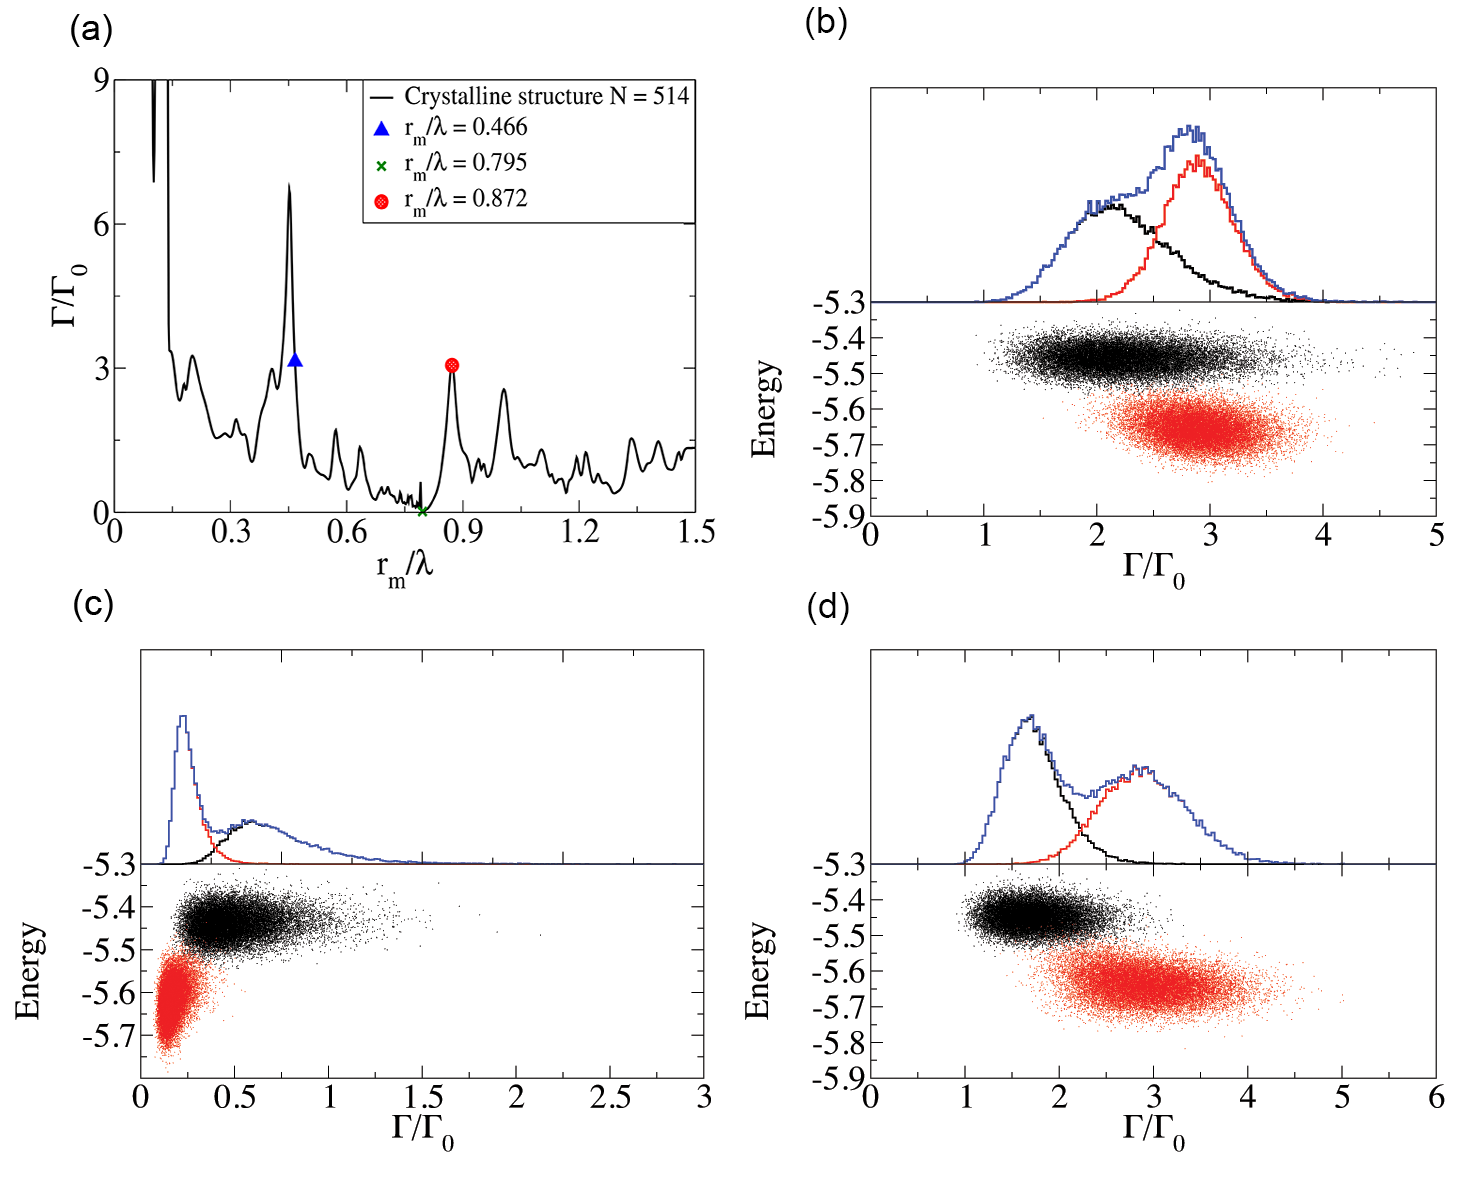
\includegraphics[width=12.5cm,angle=0]{chapter_8/figures/decay_rates.png}
\par\end{centering}
\caption{\label{fig:figm} (a) Normalized decay rates spectrum of a single emitter
placed at the center of a FCC cluster. \\
Energy-decay rate sampling at the switching region ($T\simeq0.53$, lower panels) for different ratios $r_{m}/\lambda$: (b) $r_{m}/\lambda=0.466$; (c) $r_{m}/\lambda=0.795$; (d) $r_{m}/\lambda=0.872$. Marked with symbols in (a). In the upper panels the corresponding normalized decay rates distributions are shown: red histograms correspond to the solid phase, black ones to liquid phase, and blues ones to total measured decay rates (sum of both liquid and solid distributions).}
\end{figure}

%\begin{figure}[h]
%\begin{centering}
%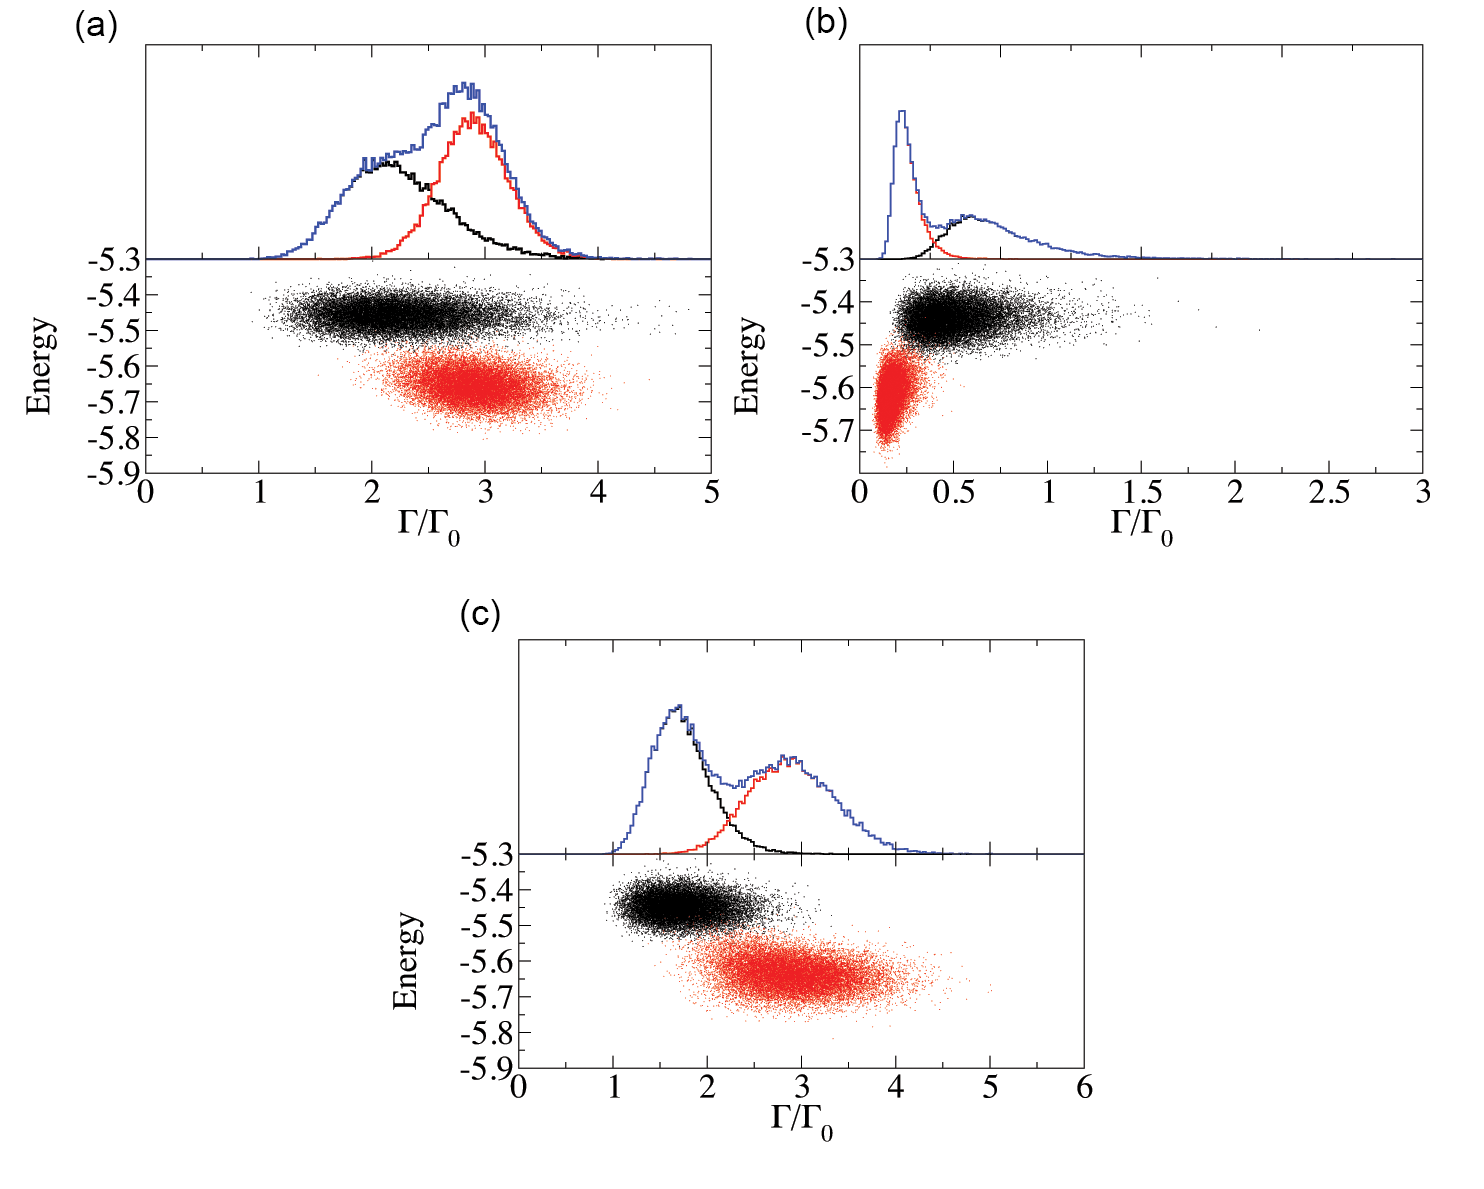
\includegraphics[width=13cm]{chapter_8/figures/image_4.png}
%\par\end{centering}
%\caption{\label{fig:fig4}Energy-decay rate sampling at the switching region
%($T\simeq0.53$, lower panels) for different ratios
%$r_{m}/\lambda$: (a) $r_{m}/\lambda=0.466$; (b) $r_{m}/\lambda=0.795$;
%(c) $r_{m}/\lambda=0.872$. Marked with symbols in Fig. \ref{fig:fig3}). In the upper panels the corresponding normalized decay rates distributions are shown: black histograms correspond to the solid phase, red ones to liquid phase, and blues ones to total measured decay rates (sum of both liquid and solid distributions).}
%\end{figure}

The statistical distributions of energy in Fig. (\ref{fig:figm})(b-d) obviously do not depend on the chosen ratios of $r_{m}/\lambda$. Although the distributions of decay rates show large variations with $r_{m}/\lambda$, there is a common feature among all the decay rate distributions: the lower energetic levels (solid phase, red distributions) are different from the higher energetic levels (liquid phase, black distributions), as seen in the upper panels. In particular its average values and fluctuations are appreciably different.\\
Measuring in a real experiment both internal energy of the interacting scatterers and the decay rate of the single emitter is far from being trivial. We might realise an experiment in which only emission lifetimes are measured for a single emitter. In this case, the only accessible quantity would be the decay rate irrespective of the value of the internal energy of the system. For the system under study, this would correspond to the added distributions plotted in blue in the upper panels of fig. (\ref{fig:figm})(b-d). Even in this case, the statistical distribution of decay rates show a signature of phase switching: Irrespective of the value of $r_{m}/\lambda$, the distributions are bimodal. \\
As mentioned, regarding the structural properties of the system in both phases in the phase-switching regime, the radial distribution functions are indistinguishable among phases, being the self-diffusion constant and the energy the only magnitudes clearly indicating that the system is in this dynamical regime. In order to clarify the origin
of the statistical signatures of phase switching in single emitter decay rates, we turn to analyse the radial distribution function of scatterers around the emitter. Our guess is that, if the diffusion of scatterers is dramatically different from one phase to the other, probably this fact has an impact on the radial distribution function and, in turn, on the statistics of decay rates.\\
In Fig. (\ref{fig:chap8_fig5}) we present the radial distribution functions (RDF) at different temperature regimes. Like before, we are able to distinguish among phases in a single MC run at constant temperature. This allow us to obtain the RDF of scatterers surrounding the emitter at liquid or at solid phases in the switching regime. The RDF is defined as the probability of finding a particle at a distance $r$ from the emitter $P\left(r\right)$ normalized by the probability in absence of any correlation $\left(\propto r^2\right)$.\\
We plot the RDF at a temperature $T \simeq 0.53$ for both the solid and the liquid  phases. Despite the fact that the two RDF among scatterers are indistinguishable, shown in Fig. (\ref{fig:chap7_Radial-distribution-function}) of the previous chapter, the RDF between scatterers and emitter is quite different. The RDF corresponding to the solid phase shows a richer structure with more pronounced peaks, while the one corresponding to the liquid phase is smoother and with wider peaks.

If we compare the RDF of the liquid phase at $T \simeq 0.53$ with the RDF
found at $T=1$, a temperature at which the system does not show phase switching and hence we call it as ''pure liquid phase'', we see that both distributions roughly coincide as shown in Fig. (\ref{fig:chap8_fig5})(b). Correspondingly, in Fig. (\ref{fig:chap8_fig5})(c) we compare the RDF of the solid phase in the phase switching regime with the RDF at $T=0.4$, which corresponds to a ''pure solid phase'' at a temperature just below the onset of the phase switching regime. We see that the RDF of the pure solid phase is also analogous to the one at the phase switching regime. In this case the correspondence is not as exact as in the liquid phase case, probably due to a stronger dependence of the RDF on the temperature for the solid phase.

\begin{figure}[H]
\begin{centering}
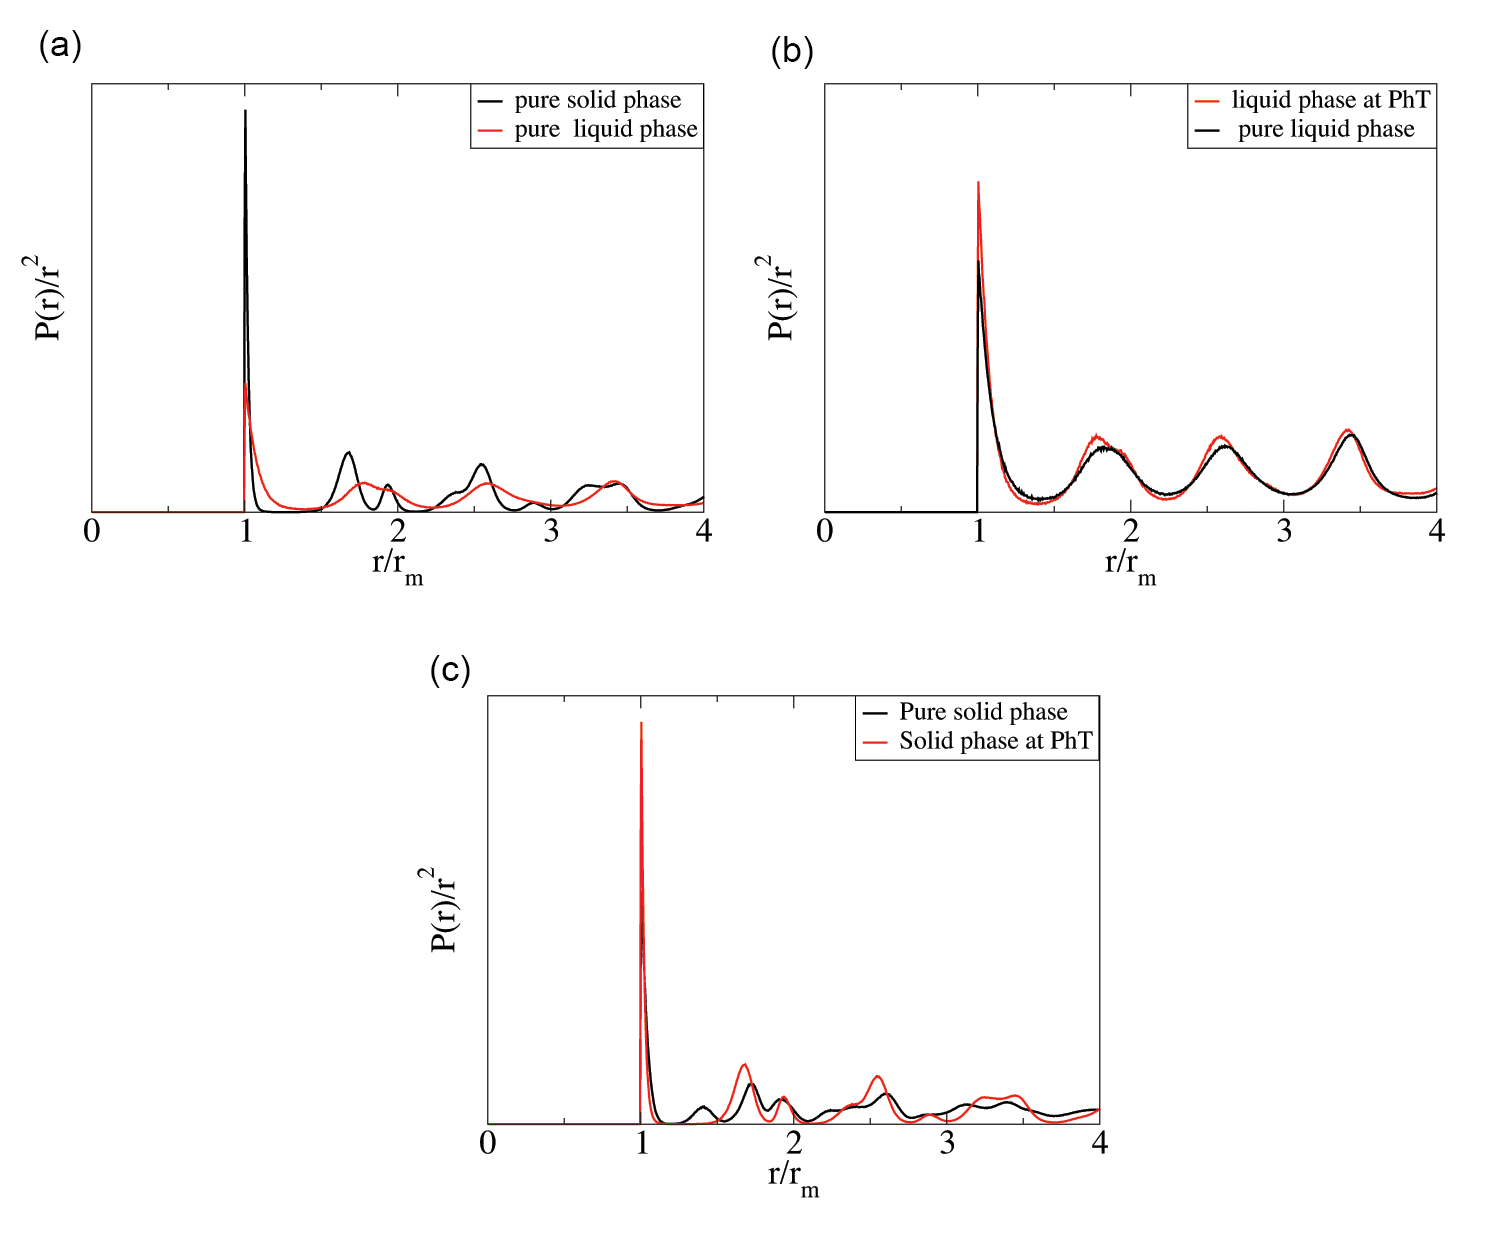
\includegraphics[width=12.5cm]{chapter_8/figures/RDF.png}
\par\end{centering}
\caption{\label{fig:chap8_fig5} Radial distribution function for scatterers surrounding the emitter placed at the center of the distribution in the phase-switching region. Liquid and solid phases are discriminated. (a) comparison of RDFs for the pure solid phase ($T =0.4$) with one in a pure liquid phase ($T=1$); (b) comparison of RDFs for the liquid phase ($T \simeq 0.53$) in the phase switching region with one in a pure liquid phase ($T=1$); (c) comparison of RDFs for the solid phase ($T \simeq 0.53$) in the phase switching region with one in a pure solid phase ($T=0.4$).}
\end{figure}



The above results suggest a relation between different decay rate statistics and structural properties of the system. The differences in the RDF can clearly be associated to the different nature of the phases, liquid or solid, as shown in the previous paragraphs. The different RDF might be the result of the large differences in the self-diffusion constant on the liquid and solid phases: in the liquid phase the scatterers can be arranged around the scatterers different ways as compared to the solid phase. It must to be noticed that the RDF among scatterers is indistinguishable and it is only the distribution of scatterers around a pinned emitter what shows differences among phases. \\
We suggest then that the above results are consistent with relatively subtle differences in the light scattering with scatterers which lie relatively close to the emitter, at distances comparable to a few wavelengths. In fact, as can be observed in Fig. (\ref{fig:chap8_fig5})(a), the RDFs for liquid and solid phases become more similar as the distance to the emitter increases, hence scatterers further apart than a few $r_{m}$ should not contribute to the differences in the decay rate statistics.

\section{Conclusion\label{sec:chap8_conclusion}}

In this chapter we have studied a model system of interacting light scatterers that present a solid-liquid phase transition. In the case where the system is relatively small (few hundreds of scatterers) and strongly confined, the system can enter in a phase switching regime where it switches among phases in its entirety in a certain range of temperatures. We have shown that, due to the fact that inter-particle RDF is indistinguishable between both phases, light scattering experiments are not able to discriminate if the system is in the switching regime. \\
Surprisingly, we find that single emitter decay-rate statistics experiments might, in principle, present strong signatures of the phase switching regime if performed in an appropriate way, in particular with low diffusivity emitters. We attribute this behaviour to the difference in the RDF between scatterers and the emitter position which, in turn, might also be attributed to differences in the self-diffusion of scatterers between both phases.\\
%The system we have considered presents an illustration of one deep difference between light scattering and light emission. 
The behaviour of this system clearly illustrates the fundamental differences between light emission statistics, (\textit{e.g.} $C_{0}$ correlations and LDOS fluctuations) and transport statistics, the former providing much more information about the statistical properties of the microstructure of the system.\\
Apart from the fundamental implications of this effect, it might be used as a tool for monitoring subtle thermodynamical behaviours of complex systems at sizes comparable with the wavelength of the light source employed in the experiment.\\
%The behaviour of this system clearly illustrates the fundamental differences between light emission statistics, (\textit{e.g.} $C_{0}$ correlations and LDOS fluctuations) and transport statistics, the former providing much more information about the statistical properties of the microstructure of the system.















                                   %Chapter 8
\chapter{Concluding remarks\label{chap9}}


Although the problems addressed in this thesis are part of very active topics in physics and engineering, we believe that many important questions remain unanswered. \\
In a significant part of this thesis we used simplified models, such as the coupled dipole model. These models have the advantage of explaining complex physical phenomena by simple principles. However, they are not as accurate as other methods when the goal is to reproduce experiments. Thus, this thesis is directed to the explanation and prediction of phenomena and not their accurate reproduction.\\
%In this thesis we tackle some open problems, presenting now the main conclusions.\\
In this chapter we present the main conclusions of our work.\\
The first part of the thesis, composed by chapters (\ref{chap3}), (\ref{chap4}) and (\ref{chap5}), is devoted to the study of light scattering phenomena in magnetoplasmonic systems, while the second part, composed by chapters (\ref{chap6}), (\ref{chap7}) and (\ref{chap8}), we study light emission statistics in random correlated systems.\\

In chapter (\ref{chap3}) we present a study of the influence of the magneto-optical activity over a nanostructure. We consider a dimer system formed by two nanodisks, one plasmonic and other magnetoplasmonic, where the electromagnetic coupling is controlled via distance between them. The system is illuminated and a magnetic field is applied perpendicularly to the surface of the nanodisks, \textit{i.e.}, in Kerr configuration.
 As consequence of the electromagnetic excitation and the application of the magnetic field, an induced net electric dipole along the perpendicular direction (perpendicular to the incident light and its polarisation direction, and to the applied magnetic field) in the magneto-optic active nanodisk is generated. Due to the interference between both nanodisks, a magneto-optical activity in the plasmonic nanodisk is induced. Also the interference of the fields from the nanodisks give rise to an electromagnetically induced magneto-optical transparency in these systems. This leads to a Fano-like spectral dependence of the MO activity.\\
In chapter (\ref{chap4}) we continue the study of dimer systems but this time presenting a detailed analysis of the interaction effects when the plasmonic or magneto-plasmonic nature of the nanodisk components is changed. We conclude that, for specific configurations, the magneto-optical response can be dominated by the induced magneto-optical activity of the purely plasmonic nanodisk. The magneto-optical activity of a system with only one of the nanodisks containing material with intrinsic magneto-optics can be even larger than that of a system composed of two magnetoplasmonic nanodisks.\\
%We tackle the problem by considering a simple dipole model, where the global phenomenology of the system is captured. The results are supported by experimental and full numerical calculations.\\
In chapter (\ref{chap5}) we present a study of the properties of an emitter in two different configurations when an external magnetic field is applied: in the presence of a single magnetoplasmonic nanoparticle and inside of a cavity formed by two magnetoplasmonic nanoparticles. Both systems, for a specific distance between the particles and the emitter, present a minimum in the radiative decay rate.
At this minimum, the presence of an external magnetic field leads to a large modification of the radiated field patterns, due to the opening of new radiation channels. The work undertaken in this chapter serves as a first approach to problems where the control of light emission is done by magneto-optical effects. \\
The study of simple magneto-optical systems like those described above, does not only explain the physics behind these specific problems, but also encourages the study of other systems. The manipulation of the geometry of the particles, shapes and sizes, separately or together, can result in a diverse and rich phenomenology. Magneto-Chiral, disordered or correlated magnetoplasmonic systems are some of the unexplored problems with great potential.

In chapter (\ref{chap6}) we study the statistical decay rate dependence of a point emitter in a system of nanoparticles statistically distributed according to a 2D lattice-gas model at different temperatures. The temperature, in this problem, is the responsible for the control of the correlations between vacancies. When the ordering temperature is far from criticality, the correlation length is small, and the decay rate distribution has the typical long-tailed shape where events with large Purcell factors are rare.
%Is shown that for short-range correlations, the Purcell factors present non-Gaussian long-tailed statistics where events with large Purcell factors are extremely rare.
For temperatures near the critical point, where the correlation length tends to infinity, the statistics evolves towards a bimodal distribution with two well-defined peaks, one at high enhancement factors, while another peak remains at values corresponding to free space. %We show that diluted systems, where vacancies are distributed in a long-range manner, enclose clusters of dipoles of all sizes, allowing for the existence of many configurations with optical modes confined around the source.\\
For diluted systems we show that it is possible that many configurations with optical modes confined around the source exist.\\
In chapter (\ref{chap7}) we study the self-diffusion of a strongly confined Lennard-Jones system. For clusters with a few hundred of particles, the system present a dynamic phase switching between solid-like and liquid-like phases. The monitoring of the self-diffusion coefficient in the solid-like and liquid-like phase in the phase-switching region, indicates a difference of a factor of three between both phases (with a larger value in the liquid-like phase). Unexpectedly, the radial distribution function in the phase-switching region is essentially indistinguishable between both phases.\\% In this way, a possible way to identify phases could be made by the analysis of the internal energy evolution or the self-diffusion characteristics of the system, because structural information does not provide a relevant signature of phase switching in this case.\\
In chapter (\ref{chap8}) we propose a method based on emission decay rate experiments to identify the different phases. Although light scattering experiments do not discriminate the system in the switching regime, single emitter decay-rate statistics experiments (with low diffusive emitters) may allow the identification of phases. This behaviour can be attributed to the difference in the radial distribution function between scatterers and the emitter which, in turn, might also be attributed to differences in the self-diffusion of scatterers between both phases. This work proposes a new way of monitor subtle thermodynamical behaviours of complex systems at sizes comparable with the wavelength of the light source employed in the experiment.\\
%The understanding of light scattering and emission through complex systems is as interesting as complex and difficult. Despite the efforts, much remains to be done. Introduction of optical forces in complex systems or experimental implementation of two and three-dimensional systems are some of the unexplored paths.
The understanding of light scattering and emission through complex systems is as interesting as complex and difficult. Despite the efforts, much remains to be done. Questions such as the importance of optical forces in complex systems or the introduction of nonreciprocal effects in disordered systems are actual open problems.
                                   %Chapter 9

\appendix
\chapter{Green Tensor}

\section{Evaluation of the Imaginary part of the Green tensor at emitter position, $\Im\left\{\mathbf{G}\left(\mathbf{r}_{0},\mathbf{r}_{0}\right)\right\}$\label{App:green_at_origin}}

The Green tensor is used to propagate the electric field generated by a point source at $\mathbf{r}_{0}$ to some point $\mathbf{r}$, represented as $\mathbf{G}\left(\mathbf{r},\mathbf{r}_{0}\right)$. To evaluate the radiated power by an emitter is necessary to calculate the imaginary part of the Green tensor at the emitter position, \textit{i.e.}, $\Im\left\{\mathbf{G}\left(\mathbf{r}_{0},\mathbf{r}_{0}\right)\right\}$. Although its evaluation seams impossible because appears to be infinite for $R = 0$, the problem can be circumvented. The key is in the expansion of the exponential term.\\
The Green tensor reads:

\begin{equation}
\mathbf{G}\left(\mathbf{r},\mathbf{r}_{0}\right) = \frac{e^{ikR}}{4\pi R}\left[\left(1+\frac{ikR-1}{k^2R^2}\right)\mathbb{I}+\frac{3-3ikR-k^2R^2}{k^2R^2}\frac{\mathbf{R} \otimes\mathbf{R}}{R^2}\right],
\end{equation}
with $R = \mathbf{r}-\mathbf{r}_{0}$ and $\frac{\mathbf{R} \otimes\mathbf{R}}{R^2} = \hat{\mathbf{R}}\otimes \hat{\mathbf{R}}$.
The imaginary part of the Green tensor for the case where $\mathbf{r} = \mathbf{r}_{0}$ is:

\begin{eqnarray*}
\Im\left\{ \mathbf{G}\left(\mathbf{r}_{0},\mathbf{r}_{0}\right)\right\}  & = & \lim_{R \rightarrow 0 }\Im\left\{ \frac{e^{ikR}}{4\pi R}\left[\left(1+\frac{ikR-1}{k^{2}R^{2}}\right)\mathbb{I}+\frac{3-3ikR-k^{2}R^{2}}{k^{2}R^{2}}\hat{\mathbf{R}}\otimes \hat{\mathbf{R}}\right]\right\} \\
\end{eqnarray*}
\begin{eqnarray*}
 & = & \lim_{R \rightarrow 0 }\Im\left\{ \frac{1}{4\pi R}\left[1+ikR-\frac{1}{2}\left(kR\right)^{2}-i\frac{1}{6}\left(kR\right)^{3}+\mathcal{O}^{4}\right]\right. \\
 & & \left. \left[\left(1+\frac{ikR-1}{k^{2}R^{2}}\right)\mathbb{I}+\frac{3-3ikR-k^{2}R^{2}}{k^{2}R^{2}}\hat{\mathbf{R}}\otimes \hat{\mathbf{R}}\right]\right\} \\
 & = & \lim_{R \rightarrow 0 } \left\{\frac{1}{4\pi R}\left[\left(\frac{ikR}{k^{2}R^{2}}+ikR-\frac{ikR}{k^{2}R^{2}}-\frac{ik^{3}R^{3}}{2k^{2}R^{2}}-i\frac{1}{6}k^{3}R^{3}+i\frac{k^{3}R^{3}}{6k^{2}R^{2}}\right)\mathbb{I}+ \right. \right. \\
 & & \left. \left. + \left(\frac{-3ikR}{k^{2}R^{2}}+\frac{3ikR}{k^{2}R^{2}}-\frac{ik^{3}R^{3}}{k^{2}R^{2}}+\frac{3ik^{3}R^{3}}{2k^{2}R^{2}}-i\frac{3k^{3}R^{3}}{6k^{2}R^{2}}+i\frac{k^{5}R^{5}}{6k^{2}R^{2}}\right)\hat{\mathbf{R}}\otimes \hat{\mathbf{R}}\right]\right\}\\\end{eqnarray*}
\begin{eqnarray*}
 & = & \lim_{R \rightarrow 0 }\left\{\frac{1}{4\pi R}\left[\left(\frac{i}{kR}+ikR-\frac{i}{kR}-\frac{ikR}{2}-i\frac{1}{6}k^{3}R^{3}+i\frac{kR}{6}\right)\mathbb{I}+ \right. \right. \\
 & & \left. \left.+ \left(\frac{-3i}{kR}+\frac{3i}{kR}-ikR+\frac{3ikR}{2}-i\frac{3kR}{6}+i\frac{k^{3}R^{3}}{6}\right)\hat{\mathbf{R}}\otimes \hat{\mathbf{R}}\right]\right\}
\end{eqnarray*}
\begin{eqnarray*}
 &  & \lim_{R \rightarrow 0 }\left\{\frac{1}{4\pi}\left[\left(\frac{i}{kR^2}-\frac{i}{kR^2}+ik-\frac{ik}{2}-i\frac{1}{6}k^{3}R^{2}+i\frac{k}{6}\right)\mathbb{I}\right.\right. \\ 
 & & \left.\left. +\left(\frac{-3i}{kR^{2}}+\frac{3i}{kR^{2}}-ik+\frac{3ik}{2}-i\frac{3k}{6}+i\frac{k^{3}R^{2}}{6}\right)\hat{\mathbf{R}}\otimes \hat{\mathbf{R}}\right]\right\}\\
  \end{eqnarray*}
 \begin{eqnarray}
 \Im\left\{ \mathbf{G}\left(\mathbf{r}_{0},\mathbf{r}_{0}\right)\right\} & = & \frac{k}{4\pi}\frac{2}{3}\mathbb{I}.
\end{eqnarray}

\section{Evaluation of the radiated power of a dipole in free space \label{App:eval_green_source}}

According with Poynting's theorem \cite{Jackson_CE}, the radiated power of a time harmonic current distribution is identical to the rate of energy dissipation:

\begin{equation}
\frac{dW}{dt}=-\frac{1}{2}\int_V^{} \Re\left\{\mathbf{j}^{*}\cdot\mathbf{E}\right\} dV.
\end{equation}
where $\mathbf{j}$ is not the total current density but instead represents the source current,  $\mathbf{j}_{s}$, that generates the fields or the loss currents,  $\mathbf{j}_{c}$, corresponding to the thermal losses and $V$ is the volume of the current distribution. If we consider the source like the one described in Eq. (\ref{eq:EM_source}), we obtain:


\begin{equation}
\frac{dW}{dt}=\frac{\omega}{2} \Im\left\{\boldsymbol{\mu}^{*}\cdot\mathbf{E}\left(\mathbf{r}_{0}\right)\right\},\label{eq:Ap1_Radiated_power}
\end{equation}
being $\mathbf{E}\left(\mathbf{r}_{0}\right)$ the electric field at dipole position at $\mathbf{r}_0$.\\
Considering the electric field (see chapter (\ref{sec:chap2_dyadic_green_function})) at point $\mathbf{r}$ as:

\begin{equation}
\mathbf{E}\left(\mathbf{r}\right) = \omega^2 \mu_{0} \mu \mathbf{G}\left(\mathbf{r},\mathbf{r}',\omega\right)\boldsymbol{\mu},
\end{equation}
Eq. (\ref{eq:Ap1_Radiated_power}) can be written as:

\begin{equation}
\frac{dW}{dt}=\frac{\omega^{3}\left|\boldsymbol{\mu}\right|^{2}}{2c^{2}\epsilon_{0}}\left[\mathbf{n}_{\mu}\cdot\Im\left\{ \mathbf{G}\left(\mathbf{r},\mathbf{r},\omega\right)\right\} \cdot\mathbf{n}_{\mu}\right],
\end{equation}
with $\mathbf{n}_{\mu}$ being the unit vector in the direction of the dipole moment. In Appendix (\ref{App:green_at_origin}) we show  how to evaluate the Green tensor at emitter position. Due to the product between $\boldsymbol{\mu}$ and $\mathbf{E}$, is necessary to evaluate the component of $\mathbf{E}$ in the direction of $\boldsymbol{\mu}$. If we place $\boldsymbol{\mu}$ in the $z-$direction (see Fig. (\ref{fig:app_axis})), $\boldsymbol{\mu} = \left|\boldsymbol{\mu}\right|\mathbf{n}_{z}$, the $z$ component of the electric field is given by:

\begin{equation}
E_z = \frac{\left|\boldsymbol{\mu}\right|}{4\pi\epsilon_{0}}\frac{e^{ikR}}{R}\left[k^2\sin^2 \theta + \frac{1}{R^2}\left(3\cos^2 \theta -1 \right) - \frac{ik}{R}\left(3 \cos^2 \theta -1\right) \right].
\end{equation}

\begin{figure}[h]
\begin{centering}

\includegraphics[width=6cm]{appendices/axis.png} 
\par\end{centering}
\caption{Schematic representation of the dipole and the corresponding field in a point in spherical coordinates, when the dipole points along the $z-$ axis.\label{fig:app_axis}}
\end{figure}
For the evaluation of the electric field at the origin of the dipole, the exponential term is expanded:

\begin{equation}
e^{ikR} = 1 + ikR - \frac{1}{2}\left(kR\right)^2  -i\frac{1}{6}\left(kR\right)^3 + \mathcal{O}^4,
\end{equation}

thus obtaining for the case where  $R \rightarrow 0$:
\begin{eqnarray}
\frac{dW}{dt} & = & \lim_{R\rightarrow0}\frac{\omega}{2}\Im\left\{ \boldsymbol{\mu}^{*}\cdot\frac{\left|\boldsymbol{\mu}\right|}{4\pi\epsilon_{0}}\frac{1}{R}\left[1+ikR+\frac{1}{2}\left(ikR\right)^{2}+\frac{1}{6}\left(ikR\right)^{3}\right]\right. \nonumber\\
 &  & \left.\left[k^{2}\sin^{2}\theta+\frac{1}{R^{2}}\left(3\cos^{2}\theta-1\right)-\frac{ik}{R}\left(3\cos^{2}\theta-1\right)\right]\right\}.
\end{eqnarray}

Considering that $\boldsymbol{\mu}$ is a real number, and only present the imaginary elements of the equation. We finally obtain:

\begin{eqnarray}
\frac{dW}{dt} & = & \frac{\left|\boldsymbol{\mu}\right|^2}{4\pi} \frac{\omega}{\epsilon_{0}}\frac{k^3}{3} \nonumber\\
 & = & \frac{\left|\boldsymbol{\mu}\right|^2}{4\pi\epsilon_{0}}\frac{k^4c}{3}.
\end{eqnarray}

%For the limit case where we obtain:
%
%\begin{equation}
%\frac{dW}{dt}=\lim_{R\rightarrow0}\frac{\omega}{2}\left|\boldsymbol{\mu}\right|\Im\left\{ E_{z}\right\} =\frac{\omega\left|\boldsymbol{\mu}\right|^{2}}{8\pi\epsilon_{0}}\lim_{R\rightarrow0}\left\{ \frac{2}{3}k^{3}+R^{2}\left(...\right)+...\right\} =\frac{\left|\boldsymbol{\mu}\right|^{2}}{12\pi}\frac{\omega}{\epsilon_{0}}k^{3},
%\end{equation}
%
%obtaining this way the radiated power by 

\section{Dipole radiation in inhomogeneous environments\label{App1:eval_dip_inh_env}}

Let us consider an emitter $\boldsymbol{\mu}$ located at $\mathbf{r} = \mathbf{r}_{0}$ surrounded by $\mathcal{N}$ dipolar particles $\mathbf{p}_n$ located at $\mathbf{r} = \mathbf{r}_{n}$ ($n = 1,...,\mathcal{N}$).

Considering the superposition principle, the total field at position $\mathbf{r}$ is given by:

\begin{equation}
\mathbf{E}\left(\mathbf{r}\right) = \frac{k^2}{\epsilon_{0}}\left[\mathbf{G}\left(\mathbf{r},\mathbf{r}_{0}\right)\cdot \boldsymbol{\mu} + \sum_{n=1}^{\mathcal{N}}\mathbf{G}\left(\mathbf{r},\mathbf{r}_{n}\right)\cdot \mathbf{p}_{n} \right].
\end{equation}
In far field, \textit{i.e.}, making the asymptotic expansion of the Green tensor $R = \left|\mathbf{r}\right| \gg \left|\mathbf{r}_{n}\right|$,  and $\mathbf{k}$ the wave vector defined by $\mathbf{k}=k \mathbf{u}_{r}$ with $\mathbf{u}_{r}=\frac{\mathbf{r}}{\left|\mathbf{r}\right|}$, the electric and magnetic field can be written as:

\begin{eqnarray}
\mathbf{E}_{n}\left(\mathbf{r}\right) & = & \frac{k^{2}}{\epsilon_{0}}\mathbf{G}\left(\mathbf{r},\mathbf{r}_{n}\right)\cdot\mathbf{p}_{n}\approx\frac{e^{ikR}}{4\pi R\epsilon_{0}}\left\{ \left(\mathbf{k}\times\mathbf{p}_{n}\right)\times\mathbf{k}\right\} e^{-i\mathbf{k}\cdot\mathbf{r}_{n}}\\
\mathbf{H}_{n}\left(\mathbf{r}\right) & = & \frac{1}{k}\sqrt{\frac{\epsilon_{0}}{\mu_{0}}}\left(\mathbf{k}\times\mathbf{E}_{n}\right)=\frac{1}{kZ}\left(\mathbf{k}\times\mathbf{E}_{n}\right),
\end{eqnarray}
where $Z=\sqrt{\mu_{0}/\epsilon_{0}}$ is the impedance.

The total power emitted will be given by:

\begin{eqnarray}
P & = & \frac{1}{2k}\int{\left(\mathbf{E}\times\mathbf{H}^{*}\right)}\cdot\left(r^{2}\sin\left(\theta\right)\right) d\theta d\phi \\
& = & \frac{1}{2Z}\int{\left|\mathbf{E}\right|^2\left[r^2\sin\left(\theta\right)\right]d\theta d\phi} \\
& = & \frac{k^{2}}{2Z\left(4\pi\epsilon_{0}\right)^{2}}\sum_{m,n}\int\left(k^{2}\mathbf{p}_{m}\cdot\mathbf{p}_{n}^{*} - \right. \nonumber\\
& & \left. -\left(\mathbf{p}_{m}\cdot\mathbf{k}\right)\left(\mathbf{p}_{n}^{*}\cdot\mathbf{k}\right)\right) e^{i\mathbf{k}\cdot\left( \mathbf{r}_{n}-\mathbf{r}_{m}\right)}\sin\left(\theta\right)d\theta d\phi.
\end{eqnarray}
The integral can be done as follows: First we consider $\theta$ as the angle measured from $\mathbf{r}_{nm}=\mathbf{r}_{n}-\mathbf{r}_{m}$. Integrating in $\phi$:

\begin{eqnarray}
& &\int\left(k^2\mathbf{p}_{m}\cdot\mathbf{p}_{n}^{*}-\left(\mathbf{p}_{m}\cdot\mathbf{k}\right)\left(\mathbf{p}_{n}^{*}\cdot\mathbf{k}\right)\right)e^{i\mathbf{k}\cdot\left(\mathbf{r}_{n}-\mathbf{r}_{m}\right)}\sin\left(\theta\right)d\theta d\phi \\
& = & k^2 2\pi \mathbf{p}_{m}\cdot\mathbf{p}_{n}^{*}\int e^{ikr_{nm}\cos\left(\theta\right)\sin\left(\theta\right)d\theta}- \nonumber \\
& & -k^2 \pi \left[ \mathbf{p}_{m} \cdot \mathbf{p}_{n}^{*} - \frac{\left(\mathbf{p}_{m}\cdot\mathbf{r}_{nm}\right)\left(\mathbf{p}_{n}^{*}\cdot\mathbf{r}_{nm}\right)}{r^{2}_{nm}}\right] \nonumber\\
& & \int \sin^{2}\left(\theta\right)e^{ikr_{nm} \cos \left(\theta\right)}\sin \left(\theta\right) d\theta \nonumber \\
& & -k^{2} 2 \pi \frac{\left(\mathbf{p}_{m}\cdot\mathbf{r}_{nm}\right)\left(\mathbf{p}_{n}^{*}\cdot\mathbf{r}_{nm}\right)}{r^{2}_{nm}} \nonumber \\
& & - \int \cos^{2}\left(\theta\right)e^{ikr_{nm} \cos \left(\theta\right)}\sin \left(\theta\right) d\theta.
\end{eqnarray}
Thus, it can be shown that the total radiated power is given by:

\begin{equation}
P = \frac{k^3}{2}\frac{1}{\epsilon_{0}\sqrt{\epsilon_{0} \mu_{0}}} \sum_{m,n}\Re \left\{ \mathbf{p}_{m}^{*}\cdot \Im \left[ \mathbf{G} \left(\mathbf{r}_{m},\mathbf{r}_{n}\right)\right]\cdot \mathbf{p}_{n} \right\}.
\end{equation}




                                %Appendix A
\chapter{Optical theorem for anisotropic particles}

Let us consider an anisotropic particle with radius $a$ characterised by a linear non-magnetic material with dielectric tensor $\mathbf{\epsilon}$.
For a harmonic fields, the electric displacement $\mathbf{D}$ inside of the particle is related with the electric field $\mathbf{E}$ through the expression $\mathbf{D}=\epsilon_{0}\boldsymbol{\epsilon}\left(\omega\right)\mathbf{E}$ and the magnetic field $\mathbf{H}=\epsilon_{0}c^2\mathbf{B}$, where $c$ is the speed of light in vacuum.\\
For Rayleigh particles ($a\ll \lambda$), the electric field induces a dipole  $\boldsymbol{\mu}=\epsilon_{0}\boldsymbol{\alpha}\left(\omega\right)\mathbf{E}_{0}$ where $\boldsymbol{\alpha}\left(\omega\right)$ is the polarisability tensor.\\
The optical theorem for anisotropic particles is deduced from the Poynting's theorem for harmonic fields: the time-average rate of work done by the external field $\mathbf{E}_{0}$ in the volume $V$ is equivalent to the sum of the dissipated and radiated powers:

\begin{equation}
\frac{1}{2}\Re\left\{\int_{V}\mathbf{J}^{*}\cdot\mathbf{E}_{0}d^3\mathbf{r}\right\}=P_{dis}+P_{rad} = P_{dis} + \frac{1}{2}\Re{\oint_{S} \mathbf{E}_{s}\times \mathbf{H}_{s}^{*}\cdot \mathbf{n}d\mathbf{s}},
\end{equation}

where $\mathbf{E}_{s}$ and $\mathbf{H}_{s}$ are the scattered fields.
The current density for dielectric particles is proportional to the polarisation vector $\mathbf{P}$ such that $\mathbf{J}=-i\omega\mathbf{P}$.\\
If the particle is uniformly polarised, $\mathbf{P}=\boldsymbol{\mu}/v=\epsilon_{0}\boldsymbol{\alpha}\mathbf{E}_{0}/v$, and we have:

\begin{eqnarray}
\frac{1}{2}\omega \Im\left\{\mathbf{E}_{0}^{\dagger}\cdot\boldsymbol{\mu}\right\}& = & P_{dis} + \frac{ck^4}{12\pi\epsilon_{0}}\left|\boldsymbol{\mu}\right|^2 = \\
\frac{1}{2}\omega \epsilon_{0} \Im\left\{\mathbf{E}_{0}^{\dagger}\boldsymbol{\alpha}\mathbf{E}_{0}\right\}& = & P_{dis} + \frac{ck^4}{12\pi}\epsilon_{0}\mathbf{E}_{0}^{\dagger}\boldsymbol{\alpha}^{\dagger}\boldsymbol{\alpha}\mathbf{E}_{0},
\end{eqnarray}

where we use the result of the total power radiated by a dipole obtained in Appendix (\ref{App:eval_green_source}). In the absence of absorption:

\begin{equation}
\frac{k^3}{6\pi}\mathbf{E}_{0}^{\dagger}\boldsymbol{\alpha}^{\dagger}\boldsymbol{\alpha}\mathbf{E}_{0} = \Im\left\{\mathbf{E}_{0}^{\dagger}\boldsymbol{\alpha}\mathbf{E}_{0}\right\} = \Im\left\{\mathbf{E}_{0}^{\dagger}\left[\boldsymbol{\alpha}^{\dagger}\left(\boldsymbol{\alpha}^{\dagger}\right)^{-1}\right]\boldsymbol{\alpha}\mathbf{E}_{0}\right\},
\end{equation}

which can be written as:

\begin{equation}
\Im\left[\boldsymbol{\mu}^{\dagger}\mathbf{M}\boldsymbol{\mu}\right]= 0;\qquad \mathbf{M}\equiv\left[\left[\boldsymbol{\alpha}^{\dagger}\right]^{-1}-i\frac{k^3}{6\pi}\mathbb{I}\right].
\end{equation}


The $\mathbf{M}$ should be hermitic, $\mathbf{M}=\mathbf{M}^{\dagger}$, since the expression should hold for any $\boldsymbol{\mu}$. In the absence of absorption the inverse of the polarisability will be:

\begin{equation}
\boldsymbol{\alpha}^{-1} = \mathbf{M} -i\frac{k^3}{6\pi}\mathbb{I}.
\end{equation}

where $\mathbf{M}$ is and arbitrary hermitic matrix. This equation represents the optical theorem for an non-absolving anisotropic particles.                                %Appendix B
\chapter{Polarisability of an ellipsoidal particle\label{App:pol_oblate_sphe}}

In this appendix we define the polarisability of an ellipsoidal particle. A detailed demonstration of the following expressions can be found in chapter (5) of Bohren and Huffman book \cite{bohren2008absorption}.\\
Let us consider a particle in vacuum, with semiaxes $a$, $b$ and $c$, like the one presented in Fig. (\ref{fig:app_ellip_part}).The particle is characterised by its dielectric tensor $\boldsymbol{\epsilon}$.\\

\begin{figure}[h!]
\begin{centering}

\includegraphics[width=7cm]{appendices/oblate.png} 
\par\end{centering}
\caption{Representation of a ellipsoidal particle. $a$, $b$ and $c$ are the particle's dimensions in the principal axes.\label{fig:app_ellip_part}}
\end{figure}
The static polarisability of an ellipsoidal particle is given by:

\begin{equation}
\boldsymbol{\alpha}_{0} = 4\pi abc \frac{\boldsymbol{\epsilon}-\mathbb{I}}{3\mathbb{I}+3\mathbb{L}\left(\boldsymbol{\epsilon}-\mathbb{I}\right)},
\end{equation}
being $\mathbb{L}$ the geometrical factors and defined by:

\begin{equation}
\mathbb{L} = \left[\begin{array}{ccc}
L_{1} & 0 & 0\\
0 & L_{2} & 0\\
0 & 0 & L_{3}
\end{array}\right].
\end{equation}

The geometrical factors can be calculated by considering the following expressions:
\begin{eqnarray}
L_{1} & = & \frac{abc}{2}\int^{\infty}_{0} \frac{dq}{\left(a^2+q\right)f\left(q\right)} \nonumber \\
L_{2} & = & \frac{abc}{2}\int^{\infty}_{0} \frac{dq}{\left(b^2+q\right)f\left(q\right)} \nonumber \\
1 & = & L_{1} + L_{2} + L_{3},
\end{eqnarray}
with $f\left(q\right) = \left\{\left(q+a^2\right)^2\left(q+b^2\right)^2\left(q+c^2\right)\right\}^{1/2}$.

An interesting case of ellipsoids are the spheroids, that have two axes of equal length, and consequently only one of the geotrical factors is independent.  Prolates and oblates ares generated by rotating an ellipse about its major and minor axis respectively. \\ In prolates we have $L_{2} = L_{3}$ and in oblates $L_{1} = L_{2}$.
Thus for a prolate spheroid ($b = c$):

\begin{eqnarray}
L_{1} & = & \frac{1-e^2}{e^2}\left(-1+\frac{1}{2e}\ln\frac{1+e}{1-e}\right)\\
 e^2& = &1-\frac{b^2}{a^2},
\end{eqnarray}

and for the oblate spheroid ($a = b$):

\begin{eqnarray}
L_{1} &=& \frac{g\left(e\right)}{2e^2}\left[\frac{\pi}{2} - \tan^{-1}g\left(e\right)\right]-\frac{g^2\left(e\right)}{2}\\
g\left(e\right) & = &\left(\frac{1-e^2}{e^2}\right)^{1/2}\\ 
e^2& = &1-\frac{c^2}{a^2}.
\end{eqnarray}

Both cases, when $e = 0$, result in a sphere.                                %Appendix C
\chapter{Coupled oscillators}

\section{Spring-mass model \label{app:coupled_masses}}

In Sec. (\ref{sec:chap3_nanoresonators}) we obtained the following matrix:

\begin{eqnarray}
\mathbf{M}\left(\begin{array}{c}
\mathbf{r}_{1}\\
\mathbf{r}_{2}
\end{array}\right) & \equiv & \left[\begin{array}{cc}
\left(\left(\Omega_{1}^{2}-\omega_{12}^{2}\right)\mathbb{\mathbb{I}}+\omega\omega_{c,1}\sigma_{2}\right) & \omega_{12}^{2}\mathbb{I}\\
\omega_{12}^{2}\mathbb{I} & \left(\left(\Omega_{2}^{2}-\omega_{12}^{2}\right)\mathbb{\mathbb{I}}+\omega\omega_{c,2}\sigma_{2}\right)
\end{array}\right]\left(\begin{array}{c}
\mathbf{r}_{1}\\
\mathbf{r}_{2}
\end{array}\right)\nonumber \\
 & = & \left(\begin{array}{c}
-\mathcal{F}_{1}\\
-\mathcal{F}_{2}
\end{array}\right),
\end{eqnarray}
where $\mathbb{I}$ is a $2\times2$ unit matrix, $\sigma_{2}$ is the $2\times2$ Pauli matrix $\left(\sigma_{2}\equiv \left(\begin{array}{cc}
0 & -i\\
i & 0
\end{array}\right)\right)$ and $\Omega_{i}^2\equiv \omega^2 -\omega_{i}^2 + i\omega \gamma_{i}$.

It can generally written as: 

\begin{equation}
\left[\begin{array}{cccc}
a & 0 & c & 0\\
0 & a & 0 & c\\
c & 0 & d & -b\\
0 & c & b & d
\end{array}\right]\left[\begin{array}{c}
x_{1}\\
y_{1}\\
x_{2}\\
y_{2}
\end{array}\right]=A\left[\begin{array}{c}
1\\
0\\
1\\
0
\end{array}\right].
\end{equation}

Therefore the solution reads:

\begin{equation}
\left[\begin{array}{c}
x_{1}\\
y_{1}\\
x_{2}\\
y_{2}
\end{array}\right]=\frac{A}{\hat{{\cal D}}}\left[\begin{array}{cccc}
ad^{2}-dc^{2}+b^{2}a & bc^{2} & c^{3}-dca & -bca\\
-bc^{2} & ad^{2}-dc^{2}+b^{2}a & bca & c^{3}-dca\\
c^{3}-dca & -bca & da^{2}-c^{2}a & a^{2}b\\
bca & c^{3}-dca & -ba^{2} & da^{2}-c^{2}a
\end{array}\right]\left[\begin{array}{c}
1\\
0\\
1\\
0
\end{array}\right],
\end{equation}

where $\hat{{\cal{D}}}=c^4-2ac^2d +a^2\left(d^2 + b^2\right)$.  This in the end five rise to:

\begin{equation}
\begin{cases}
x_{1}= & \frac{A}{\hat{{\cal D}}}\left[\left(c^{2}-ad\right)\left(c-d\right)+b^{2}a\right]\\
y_{1}= & \frac{A}{\hat{{\cal D}}}\left[-bc\left(c-a\right)\right]\\
x_{2}= & \frac{A}{\hat{{\cal D}}}\left[\left(c^{2}-ad\right)\left(c-a\right)\right]\\
y_{2}= & \frac{A}{\hat{{\cal D}}}\left[ba\left(c-a\right)\right].
\end{cases}
\end{equation}

\section{Point dipole model\label{App:coupled_oscillators}}

Let us consider a system formed by two dipoles in the presence of a magnetic field, like represented in Fig. (\ref{fig:app4_disks}). The top dipole is plasmonic and the bottom dipole is magnetoplasmonic, positioned at $\mathbf{r}_1$ and $\mathbf{r}_{2}$ respectively.
The interaction between the two dipoles is given by the Green tensor:

\begin{equation}
\mathbf{G}\left(\mathbf{r}_{1},\mathbf{r}_{2}\right) = \frac{e^{ikR}}{4\pi R}\left[\left(1+\frac{ikR-1}{k^2R^2}\right)\mathbb{I}+\frac{3-3ikR-k^2R^2}{k^2R^2}\frac{\mathbf{R} \otimes\mathbf{R}}{R^2}\right],\label{eq:app4_Green_tensor}
\end{equation}
where $\mathbf{R} = \mathbf{r}_{1} - \mathbf{r}_{2}$ and $R$ is the absolute value. \\

\begin{figure}[h!]
\begin{centering}

\includegraphics[width=7cm]{appendices/disks_app4.png} 
\par\end{centering}
\caption{Schematic representation of the system under study. The disk $1$ and $2$ are plasmonic and magnetoplasmonic disk respectively. $\mathbf{B}$ indicates the direction of the applied magnetic field.\label{fig:app4_disks}}
\end{figure}
The incident electric field on a particle $i$ originated from an ensemble of ${\cal{N}}$ particles is given by:

\begin{equation}
\mathbf{E}\left(\mathbf{r}_i\right) = \mathbf{E}_{0}\left(\mathbf{r}_i\right) + \frac{k^2}{\epsilon_{0}}\sum_{i \neq j}^{\cal{N}}\mathbf{G}\left(\mathbf{r}_i,\mathbf{r}_j\right) \mathbf{p}_j,
\end{equation}
where $\mathbf{p}_j = \epsilon_{0}\boldsymbol{\alpha}_i\mathbf{E}\left(\mathbf{r}_j\right)$ is the polarisation of particle $j$. The incident wave $\mathbf{E}_{0}\left(\bold{r}\right)=E_{0}e^{-ikz}\bold{u}_x$ is polarised along the $x-$axis and its wavevector is parallel to the $z-$axis (short axis of the particles), the polarisation of the particles lies in the $x-y$ plane:

\begin{equation}
\boldsymbol{\alpha}\left(\omega\right)=\left[\begin{array}{ccc}
\alpha_{i,xx} & \alpha_{i,xy} & 0\\
-\alpha_{i,xy} & \alpha_{i,xx}& 0\\
0 & 0 & \alpha_{i,zz}
\end{array}\right],\label{eq:app4_polarizabilitytensor}
\end{equation}
and the Green tensor that describes the interaction of the two particles (placed along $z-$axis) is diagonal and its given by:

\begin{equation}
\mathbf{G}\left(\mathbf{r}_1,\mathbf{r}_2\right) = \mathbf{G}\left(\mathbf{r}_2,\mathbf{r}_1\right) = \mathcal{G}\mathbb{I}=\frac{e^{ikd}}{4\pi d}\frac{\left(kd\right)^2+ikd-1}{\left(kd\right)^2}\mathbb{I},
\end{equation}
being $d$ the distance between the particles. One has to take into account that with the geometry described above the $z-$direction plays no role and can be excluded. The equations to deal with are:

\begin{equation}
\mathbf{M}\left[\begin{array}{c}
\mathbf{p}_{1}\\
\mathbf{p}_{2}
\end{array}\right]\equiv\left[\begin{array}{cc}
\frac{\boldsymbol{\alpha}_{1}^{-1}}{\epsilon_{0}} & -\frac{k^2}{\epsilon_{0}}\mathcal{G}\mathbb{I}\\
-\frac{k^2}{\epsilon_{0}}\mathcal{G}\mathbb{I} & \frac{\boldsymbol{\alpha}_{2}^{-1}}{\epsilon_0}
\end{array}\right]\left(\begin{array}{c}
\mathbf{p}_{1}\\
\mathbf{p}_{2}
\end{array}\right)=\left(\begin{array}{c}
\mathbf{E}_{0,1}\\
\mathbf{E}_{0,1}e^{i\delta}
\end{array}\right).
\end{equation}
where $\boldsymbol{\alpha}_i$ is the $2\times2$ $x-y$ part of the tensor described in Eq. (\ref{eq:app4_polarizabilitytensor}), $\mathbf{E}_{0,1}e^{i\delta} = \mathbf{E}_{0,2}$ and $\delta = -kd$ is the phase difference on the incoming wave due to the separation distance $d$ (normally $\delta \ll 1$).\\
We want to obtain the electric field that each particle feels, so:

\begin{equation}
\begin{bmatrix}\mathbf{E}_{1}\\
\mathbf{E}_{2}
\end{bmatrix}=\begin{bmatrix}\mathbb{I} & -k^2\mathcal{G}\boldsymbol{\alpha}_{2}\\
-k^{2}\mathcal{G}\boldsymbol{\alpha}_{1} & \mathbb{I}
\end{bmatrix}^{-1}\left[\begin{array}{c}
\mathbf{E}_{0,1}\\
\mathbf{E}_{0,2}
\end{array}\right].\label{Eq:app_D10}
\end{equation}
For the inversion, we consider the equations $\mathbf{A}=\mathcal{G}\boldsymbol{\alpha}_{2}$
and \textbf{$\mathbf{B}=\mathcal{G}\boldsymbol{\alpha}_{1}$}, with
$\tilde{\mathcal{G}}=k^{2}\mathcal{G}\left(\mathbf{r},\mathbf{r}'\right)$
\footnote{Note that $\det\left[\mathbb{I}-\mathcal{G}^{2}\boldsymbol{\alpha}_{1}\boldsymbol{\alpha}_{2}\right]=\det\left[\mathbb{I}-\mathcal{G}^{2}\boldsymbol{\alpha}_{2}\boldsymbol{\alpha}_{1}\right]$}:

\begin{equation}
\begin{bmatrix}\mathbb{I} & -\tilde{\mathcal{G}}\boldsymbol{\alpha}_{2}\\
-\tilde{\mathcal{G}}\boldsymbol{\alpha}_{1} & \mathbb{I}
\end{bmatrix}^{-1}=\frac{1}{\mathbb{I}-\tilde{\mathcal{G}}^{2}\boldsymbol{\alpha}_{1}\boldsymbol{\alpha}_{2}}\begin{bmatrix}\mathbb{I} & \tilde{\mathcal{G}}\boldsymbol{\alpha}_{2}\\
\tilde{\mathcal{G}}\boldsymbol{\alpha}_{1} & \mathbb{I}
\end{bmatrix}.
\end{equation}
Moving the determinant to the inside of the matrix:

\begin{equation}
\begin{bmatrix}\frac{\mathbb{I}}{\mathbb{I}-\tilde{\mathcal{G}}\boldsymbol{\alpha}_{1}\tilde{\mathcal{G}}\boldsymbol{\alpha}_{2}} & \frac{\tilde{\mathcal{G}}\boldsymbol{\alpha}_{2}}{\mathbb{I}-\tilde{\mathcal{G}}\boldsymbol{\alpha}_{1}\tilde{\mathcal{G}}\boldsymbol{\alpha}_{2}}\\
\frac{\mathbb{I}}{\mathbb{I}-\tilde{\mathcal{G}}\boldsymbol{\alpha}_{1}\tilde{\mathcal{G}}\boldsymbol{\alpha}_{2}} & \frac{\mathbb{I}}{\mathbb{I}-\tilde{\mathcal{G}}\boldsymbol{\alpha}_{1}\tilde{\mathcal{G}}\boldsymbol{\alpha}_{2}}
\end{bmatrix}=\begin{bmatrix}\left[\mathbb{I}-\tilde{\mathcal{G}}\boldsymbol{\alpha}_{1}\tilde{\mathcal{G}}\boldsymbol{\alpha}_{2}\right]^{-1} & \tilde{\mathcal{G}}\boldsymbol{\alpha}_{2}\left[\mathbb{I}-\tilde{\mathcal{G}}\boldsymbol{\alpha}_{1}\tilde{\mathcal{G}}\boldsymbol{\alpha}_{2}\right]^{-1}\\
\tilde{\mathcal{G}}\boldsymbol{\alpha}_{1}\left[\mathbb{I}-\tilde{\mathcal{G}}\boldsymbol{\alpha}_{1}\tilde{\mathcal{G}}\boldsymbol{\alpha}_{2}\right]^{-1} & \left[\mathbb{I}-\tilde{\mathcal{G}}\boldsymbol{\alpha}_{1}\tilde{\mathcal{G}}\boldsymbol{\alpha}_{2}\right]^{-1}
\end{bmatrix}.
\end{equation}
We can start to analyse element by element of the matrix:

\begin{eqnarray}
\left[\mathbb{I}-\mathbf{A}\mathbf{B}\right]^{-1} & = & \left[\begin{bmatrix}1 & 0\\
0 & 1
\end{bmatrix}-\tilde{\mathcal{G}}^{2}\begin{bmatrix}\alpha_{2xx} & \alpha_{2xy}\\
\alpha_{2yx} & \alpha_{2yy}
\end{bmatrix}\begin{bmatrix}\alpha_{1} & 0\\
0 & \alpha_{1}
\end{bmatrix}\right]^{-1} \nonumber\\
\left[\mathbb{I}-\mathbf{A}\mathbf{B}\right]^{-1} & = & \begin{bmatrix}1-\tilde{\mathcal{G}}^{2}\alpha_{1}\alpha_{2xx} & -\tilde{\mathcal{G}}^{2}\alpha_{1}\alpha_{2xy}\\
-\tilde{\mathcal{G}}^{2}\alpha_{1}\alpha_{2yx} & 1-\tilde{\mathcal{G}}^{2}\alpha_{1}\alpha_{2yy}
\end{bmatrix}^{-1}. \label{eq:app4_common_matrix}
\end{eqnarray}
Due to the symmetry of the problem ($\alpha_{2xy}=-\alpha_{2yx}$;
$\alpha_{2xx}=\alpha_{2yy}$):

\begin{equation}
\left[\mathbb{I}-\mathbf{A}\mathbf{B}\right]^{-1}=\begin{bmatrix}1-\tilde{\mathcal{G}}^{2}\alpha_{1}\alpha_{2xx} & -\tilde{\mathcal{G}}^{2}\alpha_{1}\alpha_{2xy}\nonumber\\
\tilde{\mathcal{G}}^{2}\alpha_{1}\alpha_{2xy} & 1-\tilde{\mathcal{G}}^{2}\alpha_{1}\alpha_{2xx}
\end{bmatrix}^{-1}.\label{eq:app4_common_matrix}
\end{equation}
We can write the matrix elements as:

\begin{equation}
\left[\mathbb{I}-\mathbf{A}\mathbf{B}\right]^{-1}=\frac{1}{\mathcal{D}}\begin{bmatrix}1-\tilde{\mathcal{G}}^{2}\alpha_{1}\alpha_{2xx} & \tilde{\mathcal{G}}^{2}\alpha_{1}\alpha_{2xy}\\
-\tilde{\mathcal{G}}^{2}\alpha_{1}\alpha_{2xy} & 1-\tilde{\mathcal{G}}^{2}\alpha_{1}\alpha_{2xx}
\end{bmatrix},
\end{equation}

\begin{eqnarray}
\mathbf{A}\left[\mathbb{I}-\mathbf{A}\mathbf{B}\right]^{-1} & = & \tilde{\mathcal{G}}\begin{bmatrix}\alpha_{2xx} & \alpha_{2xy}\\
-\alpha_{2xy} & \alpha_{2xx}
\end{bmatrix}\begin{bmatrix}1-\tilde{\mathcal{G}}^{2}\alpha_{1}\alpha_{2xx} & \tilde{\mathcal{G}}^{2}\alpha_{1}\alpha_{2xy}  \\
-\tilde{\mathcal{G}}^{2}\alpha_{1}\alpha_{2xy} & 1-\tilde{\mathcal{G}}^{2}\alpha_{1}\alpha_{2xx}
\end{bmatrix} \nonumber\\
& = & \left[\begin{array}{c}
\tilde{\mathcal{G}}\alpha_{2xx}-\tilde{\mathcal{G}}^{3}\alpha_{1}\alpha_{2xx}^{2}-\tilde{\mathcal{G}}^{3}\alpha_{1}\alpha_{2xy}^{2}\\
-\tilde{\mathcal{G}}\alpha_{2xy}
\end{array}\right.\vdots \nonumber\\
& &\vdots\left.\begin{array}{c}
\tilde{\mathcal{G}}\alpha_{2xy}\\
\tilde{\mathcal{G}}\alpha_{2xx}-\tilde{\mathcal{G}}^{3}\alpha_{1}\alpha_{2xy}^{2}-\tilde{\mathcal{G}}^{3}\alpha_{1}\alpha_{2xx}^{2}
\end{array}\right],
\end{eqnarray}

\begin{eqnarray}
\mathbf{B}\left[\mathbb{I}-\mathbf{A}\mathbf{B}\right]^{-1} & = & \tilde{\mathcal{G}}\begin{bmatrix}\alpha_{1} & 0\\
0 & \alpha_{1}
\end{bmatrix}\begin{bmatrix}1-\tilde{\mathcal{G}}^{2}\alpha_{1}\alpha_{2xx} & \tilde{\mathcal{G}}^{2}\alpha_{1}\alpha_{2xy}\\
-\tilde{\mathcal{G}}^{2}\alpha_{1}\alpha_{2xy} & 1-\tilde{\mathcal{G}}^{2}\alpha_{1}\alpha_{2xx}
\end{bmatrix}\\
 & = & \begin{bmatrix}\tilde{\mathcal{G}}\alpha_{1}-\tilde{\mathcal{G}}^{3}\alpha_{1}^{2}\alpha_{2xx} & \tilde{\mathcal{G}}^{3}\alpha_{1}\alpha_{2xy}\\
-\tilde{\mathcal{G}}^{3}\alpha_{1}^{2}\alpha_{2xy} & \tilde{\mathcal{G}}\alpha_{1}-\tilde{\mathcal{G}}^{3}\alpha_{1}^{2}\alpha_{2xx}
\end{bmatrix},
\end{eqnarray}
and the determinant of the \ref{eq:app4_common_matrix} matrix is:

\begin{eqnarray}
\mathcal{D} & = & \left(1-\tilde{\mathcal{G}}^{2}\alpha_{1}\alpha_{2xx}\right)^{2}+\left(\tilde{\mathcal{G}}^{2}\alpha_{1}\alpha_{2xy}\right)^{2}\\
\mathcal{D} & = & 1-\left(2\tilde{\mathcal{G}}^{2}\alpha_{1}\alpha_{2xx}\right)+\tilde{\mathcal{G}}^{4}\alpha_{1}^{2}\alpha_{2xx}^{2}+\tilde{\mathcal{G}}^{4}\alpha_{1}^{2}\alpha_{2xy}^{2}\\
\mathcal{D} & = & 1-2\tilde{\mathcal{G}}^{2}\alpha_{1}\alpha_{2xx}+\tilde{\mathcal{G}}^{4}\alpha_{1}^{2}\left(\alpha_{2xx}^{2}+\alpha_{2xy}^{2}\right).
\end{eqnarray}

We can finally write:

\begin{equation}
\begin{bmatrix}\left[\mathbb{I}-\tilde{\mathcal{G}}\boldsymbol{\alpha}_{1}\tilde{\mathcal{G}}\boldsymbol{\alpha}_{2}\right]^{-1} & \tilde{\mathcal{G}}\boldsymbol{\alpha}_{2}\left[\mathbb{I}-\tilde{\mathcal{G}}\boldsymbol{\alpha}_{1}\tilde{\mathcal{G}}\boldsymbol{\alpha}_{2}\right]^{-1}\\
\tilde{\mathcal{G}}\boldsymbol{\alpha}_{1}\left[\mathbb{I}-\tilde{\mathcal{G}}\boldsymbol{\alpha}_{1}\tilde{\mathcal{G}}\boldsymbol{\alpha}_{2}\right]^{-1} & \left[\mathbb{I}-\tilde{\mathcal{G}}\boldsymbol{\alpha}_{1}\tilde{\mathcal{G}}\boldsymbol{\alpha}_{2}\right]^{-1}
\end{bmatrix}=
\end{equation}

\begin{eqnarray}
& = & \left[\begin{array}{cc}
1-\tilde{\mathcal{G}}\alpha_{1}\alpha_{2xx} & \tilde{\mathcal{G}}^{2}\alpha_{1}\alpha_{2xx}\\
-\tilde{\mathcal{G}}^{2}\alpha_{1}\alpha_{2xy} & 1-\tilde{\mathcal{G}}^{2}\alpha_{1}\alpha_{2xx}\\
\tilde{\mathcal{G}}\alpha_{1}-\tilde{\mathcal{G}}^{3}\alpha_{1}^{2}\alpha_{2xx} & \tilde{\mathcal{G}}^{3}\alpha_{1}^{2}\alpha_{2xy}\\
-\tilde{\mathcal{G}}^{3}\alpha_{1}^{2}\alpha_{2xy} & \tilde{\mathcal{G}}\alpha_{1}-\tilde{\mathcal{G}}^{3}\alpha_{1}^{2}\alpha_{2xx}
\end{array}\right. \vdots \nonumber\\
& &
\vdots\left.\begin{array}{cc}
\tilde{\mathcal{G}}\alpha_{2xx}-\tilde{\mathcal{G}}^{3}\alpha_{1}\alpha_{2xx}^{2}-\tilde{\mathcal{G}}^{3}\alpha_{1}\alpha_{2xy}^{2} & \tilde{\mathcal{G}}\alpha_{2xy}\\
-\tilde{\mathcal{G}}\alpha_{2xy} & \tilde{\mathcal{G}}\alpha_{2xx}-\tilde{\mathcal{G}}^{3}\alpha_{1}\alpha_{2xy}^{2}-\tilde{\mathcal{G}}^{3}\alpha_{1}\alpha_{2xx}^{2}\\
1-\tilde{\mathcal{G}}^{2}\alpha_{1}\alpha_{2xx} & \tilde{\mathcal{G}}^{2}\alpha_{1}\alpha_{2xy}\\
-\tilde{\mathcal{G}}^{2}\alpha_{1}\alpha_{2xy} & 1-\tilde{\mathcal{G}}^{2}\alpha_{1}\alpha_{2xx}
\end{array}\right]. \nonumber
\end{eqnarray}
So:

\begin{equation}
\begin{bmatrix}\mathbf{p}_{1}\\
\mathbf{p}_{2}
\end{bmatrix}=\epsilon_{0}\begin{bmatrix}\boldsymbol{\alpha}_{1} & 0\\
0 & \boldsymbol{\alpha}_{2}
\end{bmatrix}\begin{bmatrix}\mathbf{E}_{1}\\
\mathbf{E}_{2}
\end{bmatrix}=\epsilon_{0}\begin{bmatrix}\boldsymbol{\alpha}_{1} & 0\\
0 & \boldsymbol{\alpha}_{2}
\end{bmatrix}\begin{bmatrix}\mathbb{I} & -\tilde{\mathcal{G}}\boldsymbol{\alpha}_{2}\\
-\tilde{\mathcal{G}}\boldsymbol{\alpha}_{1} & \mathbb{I}
\end{bmatrix}\begin{bmatrix}\mathbf{E}_{1}\\
\mathbf{E}_{2}
\end{bmatrix}\nonumber
\end{equation}

Considering Eq. (\ref{Eq:app_D10}) in the previous equation, we obtain:

\begin{equation}
\begin{bmatrix}\mathbf{p}_{1}\\
\mathbf{p}_{2}
\end{bmatrix}=\epsilon_{0}\begin{bmatrix}\boldsymbol{\alpha}_{1} & 0\\
0 & \boldsymbol{\alpha}_{2}
\end{bmatrix}\begin{bmatrix}\mathbb{I} & -\tilde{\mathcal{G}}\boldsymbol{\alpha}_{2}\\
-\tilde{\mathcal{G}}\boldsymbol{\alpha}_{1} & \mathbb{I}
\end{bmatrix}^{-1}\left[\begin{array}{c}
\mathbf{E}_{0,1}\\
\mathbf{E}_{0,2}
\end{array}\right].\nonumber
\end{equation}

\[
\begin{bmatrix}\mathbf{p}_{1}\\
\mathbf{p}_{2}
\end{bmatrix}=\frac{\epsilon_{0}}{\mathcal{D}}\left[\begin{array}{c}
\alpha_{1}\left(1-\tilde{\mathcal{G}}^{2}\alpha_{1}\alpha_{2xx}\right)\\
-\tilde{\mathcal{G}}^{2}\alpha_{1}^{2}\alpha_{2xy}\\
\tilde{\mathcal{G}}\alpha_{1}\left[\alpha_{2xx}-\tilde{\mathcal{G}}^{2}\alpha_{1}\left(\alpha_{2xx}^{2}+\alpha_{2xy}^{2}\right)\right]\\
-\tilde{\mathcal{G}}\alpha_{1}\alpha_{2xy}
\end{array}\vdots\right.
\]

\[
\vdots\begin{array}{c}
\tilde{\mathcal{G}}^{2}\alpha_{1}^{2}\alpha_{2xy}\\
\alpha_{1}-\tilde{\mathcal{G}}^{2}\alpha_{1}^{2}\alpha_{2xx}\\
\tilde{\mathcal{G}}\alpha_{1}\alpha_{2xy}\\
\tilde{\mathcal{G}}\alpha_{1}\left[\alpha_{2xx}-\tilde{\mathcal{G}}^{2}\alpha_{1}\left(\alpha_{2xx}^{2}+\alpha_{2xy}^{2}\right)\right]
\end{array}\vdots
\]

\[
\vdots\begin{array}{c}
\tilde{\mathcal{G}}\alpha_{1}\left[\alpha_{2xx}-\tilde{\mathcal{G}}^{2}\alpha_{1}\left(\alpha_{2xx}^{2}+\alpha_{2xy}^{2}\right)\right]\\
-\tilde{\mathcal{G}}\alpha_{1}\alpha_{2xy}\\
\left[\alpha_{2xx}-\tilde{\mathcal{G}}^{2}\alpha_{1}\left(\alpha_{2xx}^{2}+\alpha_{2xy}^{2}\right)\right]\\
-\alpha_{2xy}
\end{array}\vdots
\]

\[
\left.\vdots\begin{array}{c}
\tilde{\mathcal{G}}\alpha_{1}\alpha_{2xy}\\
\tilde{\mathcal{G}}\alpha_{1}\left[\alpha_{2xx}-\tilde{\mathcal{G}}^{2}\alpha_{1}\left(\alpha_{2xx}^{2}+\alpha_{2xy}^{2}\right)\right]\\
\alpha_{2xy}\\
\left[\alpha_{2xx}-\tilde{\mathcal{G}}^{2}\alpha_{1}\left(\alpha_{2xx}^{2}+\alpha_{2xy}^{2}\right)\right]
\end{array}\right]\begin{bmatrix}E_{0,1x}\\
E_{0,1y}\\
E_{0,2x}\\
E_{0,2y}
\end{bmatrix}.
\]

So, we can write the polarisation as:

\[
\begin{cases}
p_{1x}= & \frac{\epsilon_{0}}{\mathcal{D}}\left[\alpha_{1}\left(1-\tilde{\mathcal{G}}^{2}\alpha_{1}\alpha_{2xx}\right)E_{0,1x}+\left(\tilde{\mathcal{G}}^{2}\alpha_{1}^{2}\alpha_{2xy}\right)E_{0,1y}+\right.\\
 & \left.+\tilde{\mathcal{G}}\alpha_{1}\left[\alpha_{2xx}-\tilde{\mathcal{G}}^{2}\alpha_{1}\left(\alpha_{2xx}^{2}+\alpha_{2xy}^{2}\right)\right]E_{0,2x}+\tilde{\mathcal{G}}\alpha_{1}\alpha_{2xy}E_{0,2y}\right]\\
p_{1y}= & \frac{\epsilon_{0}}{\mathcal{D}}\left[-\tilde{\mathcal{G}}^{2}\alpha_{1}^{2}\alpha_{2xy}E_{0,1x}+\left(\alpha_{1}-\tilde{\mathcal{G}}^{2}\alpha_{1}^{2}\alpha_{2xx}\right)E_{0,1y}-\right.\\
 & \left.-\tilde{\mathcal{G}}\alpha_{1}\alpha_{2xy}E_{0,2x}+\tilde{\mathcal{G}}\alpha_{1}\left[\alpha_{2xx}-\tilde{\mathcal{G}}^{2}\alpha_{1}\left(\alpha_{2xx}^{2}+\alpha_{2xy}^{2}\right)\right]E_{0,2y}\right]\\
p_{2x}= & \frac{\epsilon_{0}}{\mathcal{D}}\left[\tilde{\mathcal{G}}\alpha_{1}\left[\alpha_{2xx}-\tilde{\mathcal{G}}^{2}\alpha_{1}\left(\alpha_{2xx}^{2}+\alpha_{2xy}^{2}\right)\right]E_{0,1x}+\tilde{\mathcal{G}}\alpha_{1}\alpha_{2xy}E_{0,1y}+\right.\\
 & \left.+\left[\alpha_{2xx}-\tilde{\mathcal{G}}^{2}\alpha_{1}\left(\alpha_{2xx}^{2}+\alpha_{2xy}^{2}\right)\right]E_{0,2x}+\alpha_{2xy}E_{0,2y}\right]\\
p_{2y}= & \frac{\epsilon_{0}}{\mathcal{D}}\left[-\tilde{\mathcal{G}}\alpha_{1}\alpha_{2xy}E_{0,1x}+\tilde{\mathcal{G}}\alpha_{1}\left[\alpha_{2xx}-\tilde{\mathcal{G}}^{2}\alpha_{1}\left(\alpha_{2xx}^{2}+\alpha_{2xy}^{2}\right)\right]E_{0,1y}+\right.\\
 & \left.-\alpha_{2xy}E_{0,2x}+\left[\alpha_{2xx}-\tilde{\mathcal{G}}^{2}\alpha_{1}\left(\alpha_{2xx}^{2}+\alpha_{2xy}^{2}\right)\right]E_{0,2y}\right],
\end{cases}
\]
and finally we obtain:

\[
\begin{cases}
p_{1x}= & \epsilon_{0}\frac{E_{0,1x}}{\mathcal{D}}\alpha_{1}\left[1+k^2\mathcal{G}\alpha_{2xx}\left[e^{i\delta}-k^2\mathcal{G}\alpha_{1}\right]-k^6\mathcal{G}^{3}\alpha_{1}\left(\alpha_{2xx}^{2}+\alpha_{2xy}^{2}\right)e^{i\delta}\right]\\
p_{1y}= & -\epsilon_{0}\frac{E_{0,1x}}{\mathcal{D}}k^2\mathcal{G}\alpha_{1}\alpha_{2xy}\left[k^2\mathcal{G}\alpha_{1}+e^{i\delta}\right]\\
p_{2x}= & \epsilon_{0}\frac{E_{0,1x}}{\mathcal{D}}\left[\alpha_{2xx}-k^4\mathcal{G}^{2}\alpha_{1}\left(\alpha_{2xx}^{2}+\alpha_{2xy}^{2}\right)\right]\left[k^2\mathcal{G}\alpha_{1}+e^{i\delta}\right]\\
p_{2y}= & -\epsilon_{0}\frac{E_{0,1x}}{\mathcal{D}}\alpha_{2xy}\left[k^2\mathcal{G}\alpha_{1}+e^{i\delta}\right],
\end{cases}
\]
with where $\mathcal{D} = 1 - 2k^4\mathcal{G}^2\alpha_{1}\alpha_{2xx}+k^8\mathcal{G}^4\alpha_1^2\left(\alpha_{2xx}^2+ \alpha_{2xy}^2\right)$.
                                %Appendix D
\chapter{Radial distribution function\label{App:Radial_distribution_function}}

Th radial distribution function, RDF or $g\left(r\right)$, is an elementary tool used to obtain structural information. \\
In chapter (\ref{chap7}) we present a numerical evaluation of the radial distribution function for systems with different correlations. In this appendix we show the used procedure. \\
The radial distribution function, from the numerical point of view, is determined by calculating the distance between all particle pairs and binning them into a histogram. The histogram is then normalized with respect to an ideal gas, where particle histograms are completely uncorrelated. For an uncorrelated system, the histogram can be expressed as follows.

Let us consider a first sphere with radius $R$, like schematically represented in Fig. (\ref{fig:app_sphere}). A second sphere, with radius $\rho$ and centred at distance $r$ from the centre of the first, is added to the system. 
%To evaluate the radial distribution we have to know the probability of find two particles at a distance $d$.
%The idea is to evaluate the of the surface 
%. This probability is given by the ratio between the surface area inside of the secondary inside the primary sphere by the total volume of the primary sphere. Let us consider a second sphere with center inside of the first sphere. The surface of this second sphere that is inside of the primary sphere is given by:
So, for any radius of the second sphere, the part of the surface that is embedded in the first sphere is given by:

\begin{equation}
S=2\pi\rho^{2}\int_{\theta_{2}}^{\pi}d\theta\sin\theta=2\pi\rho^{2}\left(1+\cos\theta_{2}\right).
\end{equation}

\begin{figure}[h!]
\begin{centering}

\includegraphics[width=8cm]{appendices/sphere_scheme.png} 
\par\end{centering}
\caption{Schematic representation of the sphere and its dimensions.\label{fig:app_sphere}}
\end{figure}
From the analysis of the Fig. (\ref{fig:app_sphere}), we can define the following equalities:

\begin{eqnarray}
R\sin\theta_{1} & = & \rho\sin\theta_{2} \nonumber\\
R\cos\theta_{1} & = & r+\rho\cos\theta_{2}
\end{eqnarray}
\begin{eqnarray}
R^{2}& = & \rho^{2}+r^{2}+2r\rho\cos\theta_{2}=\cos\theta_{2}=\frac{R^{2}-\rho^{2}-r^{2}}{2r\rho}\\
1+\cos\theta_{2}&=&\frac{R^{2}-\left(r-\rho\right)^{2}}{2r\rho}.
\end{eqnarray}

The probability of find a particle at some distance $r$ from the center of the first sphere is:

\begin{equation}
P\left(r\right)=\frac{4\pi r^2}{\left(4/3\right)\pi R^{3}}=\frac{3r^2}{R^3}.
\end{equation}

Now, the problem is divided in two parts. The first case, where $\left(\rho\leq R\right)$ and the second case, where $\left(\rho\geq R\right)$.

Case 1 $\left(\rho\leq R\right)$:

For the situation where $R\geq r + \rho$, \textit{i.e.}, the case where the second is totally inside of the primary sphere, the surface of the second sphere is given by: 

\begin{equation}
S\left(\rho,r\right)=4\pi\rho^{2}\qquad if\ R\geq r+\rho\rightarrow R-\rho\geq r\geq 0 \nonumber
\end{equation}

If only part of the second sphere is inside of the first sphere, $R<r+\rho$, the surface of second sphere embedded is:

\begin{equation}
S\left(\rho,r\right)=\pi\frac{\rho}{r}\left[R^{2}-\left(r-\rho\right)^{2}\right]\qquad R<r+\rho\rightarrow R-\rho<r.
\end{equation}

So, the probability of have any two particles at distance $\rho$ is given by:

\begin{eqnarray}
P\left(\rho\right) & \propto & \int_{0}^{R}S\left(\rho,r\right)P\left(r\right)dr\\
& \propto & \frac{3}{R^{3}}\left[\int_{0}^{R-\rho}dr4\pi r^{2}\rho^{2}+\int_{R-\rho}^{R}dr\pi\rho r\left[R^{2}-\left(r-\rho\right)^{2}\right]\right]\\
& \propto & \int_{0}^{R}S\left(\rho,r\right)P\left(r\right)dr=\frac{3}{R^{3}}\left[\int_{0}^{R-\rho}dr4\pi r^{2}\rho^{2}+\right.\nonumber\\
 & &\left.\int_{R-\rho}^{R}dr\pi\rho r\left[R^{2}-R^{2}-\rho^{2}+2r\rho-r^{2}\right]\right]\\
 & \propto & \int_{0}^{R}S\left(\rho,r\right)P\left(r\right)dr=\frac{3}{R^{3}}\left[\int_{0}^{R-\rho}dr4\pi r^{2}\rho^{2}+\right.\nonumber\\
 & &\left.\int_{R-\rho}^{R}dr\pi\rho r\left[R^{2}-R^{2}-\rho^{2}+2r\rho-r^{2}\right]\right]\\
 & \propto & \frac{3}{R^{3}}\left[\frac{4}{3}\pi\rho^{2}\left(R-\rho\right)^{3}+\frac{\pi\rho\left(R^{2}-\rho^{2}\right)}{2}\left[R^{2}-\left(R-\rho\right)^{2}\right]+\right.\nonumber\\
& & \left. \frac{2\pi\rho^{2}}{3}\left[R^{3}-\left(R-\rho\right)^{3}\right] -\frac{\pi\rho}{4}\left[R^{4}-\left(R-\rho\right)^{4}\right]\right]\\
P\left(\rho\right)& \propto & \frac{\pi}{4R^{3}}\left\{ 16\rho^{2}\left(R-\rho\right)^{3}+6\rho\left(R^{2}-\rho^{2}\right)\left[R^{2}-\left(R-\rho\right)^{2}\right]+\right.\nonumber\\
& &\left. +8\rho^{2}\left[R^{3}-\left(R-\rho\right)^{3}\right]-3\rho\left[R^{4}-\left(R-\rho\right)^{4}\right]\right\}.
\end{eqnarray}
%\begin{equation}
%If\ \rho=R\rightarrow P\left(\rho=R\right)=\frac{\pi}{4R^{3}}\left(8R^{5}-3R^{5}\right)=\frac{5}{4}\pi R^{2}
%\end{equation}

Case 2 $\left(\rho\geq R\right)$:

For the situation where $R\geq r - \rho$: 


 $\left(\rho\geq R\right)\ if\ \rho-r\leq R\rightarrow S\left(\rho,r\right)=\pi\frac{\rho}{R}\left[R^{2}-\left(r-\rho\right)^{2}\right]$

\[
\rho-r\geq R\rightarrow S\left(\rho,r\right)=0
\]


\[
P\left(\rho\right)\propto\frac{3\pi\rho}{R^{3}}\int_{\rho-R}^{R}\left\{ \left(R^{2}-\rho^{2}\right)r+2\rho r^{2}-r^{3}\right\} 
\]


\begin{eqnarray}
& \propto & \frac{3\pi\rho\left(R^{2}-\rho^{2}\right)}{2R^{3}}\left[R^{2}-\left(\rho-R\right)^{2}\right]+\nonumber\\
& & +\frac{2\pi\rho^{2}}{R^{3}}\left[R^{3}-\left(\rho-R\right)^{3}\right]-\frac{3\pi\rho}{4R^{3}}\left[R^{4}-\left(\rho-R\right)^{4}\right]
\end{eqnarray}


\begin{eqnarray}
P\left(\rho\right) & \propto &\frac{\pi\rho}{4R^{3}}\left\{ -3R^{4}+3\left(\rho-R\right)^{4}+8\rho\left[R^{3}-\left(\rho-R\right)^{3}\right]+\right.\nonumber\\
& & \left.+6\left(R^{2}-\rho^{2}\right)\left[R^{2}-\left(\rho-R\right)^{2}\right]\right\}.
\end{eqnarray}

So, we can finally write:

\begin{equation}
P\left(\rho\right) = \begin{cases}
 & \frac{3}{4\pi R^3}\frac{\pi}{4R^{3}}\left\{ 16\rho^{2}\left(R-\rho\right)^{3}+6\rho\left(R^{2}-\rho^{2}\right)\left[R^{2}-\left(R-\rho\right)^{2}\right]+\right.\\
&\left. +8\rho^{2}\left[R^{3}-\left(R-\rho\right)^{3}\right]-3\rho\left[R^{4}-\left(R-\rho\right)^{4}\right]\right\}  \quad \rho \le R\\
&\\ 
  &\frac{3}{4\pi R^3} \frac{\pi\rho}{4R^{3}}\left\{ -3R^{4}+3\left(\rho-R\right)^{4}+8\rho\left[R^{3}-\left(\rho-R\right)^{3}\right]+\right.\nonumber\\
& \left.+6\left(R^{2}-\rho^{2}\right)\left[R^{2}-\left(\rho-R\right)^{2}\right]\right\} \quad \rho \ge R.
\end{cases}
\end{equation}

In Fig. (\ref{fig:app_uncorrelated}) we present the normalized histogram of a system with radius $R = 1$.

\begin{figure}[h!]
\begin{centering}

\includegraphics[width=7cm, angle=-90]{appendices/uncorrelated.eps} 
\par\end{centering}
\caption{Normalised histogram of the distance between all particle pairs for a sphere with $R = 1$.\label{fig:app_uncorrelated}}
\end{figure}



%If $\rho=R^{+}\rightarrow P\left(\rho=R^{+}\right)=\frac{\pi R}{4R^{3}}\left\{ -3R^{4}+8R^{4}\right\} =\frac{5}{4}\pi R^{2}$

%That coincids with the other result $\rho=R^{-}$                                %Appendix E
\chapter{Conclusiones Generales\label{App:Conclusiones_gen}}

Aunque los problemas abordados en esta tesis forman parte de temas muy comunes en f�sica e ingenier�a, creemos que muchas cuestiones importantes est�n a�n sin responder. \\
En una gran parte de la tesis hemos utilizado modelos sencillos, como el modelo de dipolos acoplados. Estos modelos tienen la ventaja de poder explicar fen�menos complejos de la f�sica atrav�s de principios b�sicos. Sin embargo, no son tan precisos como otros m�todos cuando se pretende reproducir experimentos. Por lo tanto, esta tesis est� encaminada hacia la explicaci�n y predicci�n de los fen�menos y no su reproducci�n. \\
En este cap�tulo se presentan las principales conclusiones de nuestro trabajo. 
En la primera parte de la tesis, compuesta por los cap�tulos (\ref{chap3}), (\ref{chap4}) y (\ref{chap5}), se estudian los fen�menos de scattering de luz en sistemas magnetoplasm�nicos, mientras que en la segunda parte, compuesta por los cap�tulos (\ref{chap6}), (\ref{chap7}) y (\ref{chap8}), se estudian las estad�sticas de emisi�n de luz en los sistemas aleatorios correlacionados. 

En el cap�tulo (\ref{chap3}) se explica la influencia de la actividad magneto-�ptica sobre un sistema formado por dos nanodiscos, uno plasm�nico y otro magnetoplasm�nico, entre los cuales el acoplamiento electromagn�tico se controla a trav�s de la distancia entre ellos. El sistema se ilumina y se le aplica un campo magn�tico, ambos de forma perpendicular perpendicular a la superficie de los nanodiscos,  \textit{i.e.}, en la configuraci�n Kerr. Como consecuencia de la excitaci�n electromagn�tica y la aplicaci�n del campo magn�tico, se genera un dipolo el�ctrico, perpendicular a la luz incidente, a su direcci�n de polarizaci�n y al campo magn�tico aplicado, en el nanodisco magneto-�pticamente activo. Debido a la interferencia entre ambos nanodiscos, se induce una actividad magneto-�ptica en el disco plasm�nico. Como consecuencia de la interferencia de los campos de los nanodiscos, se observa la existencia de transparencia magneto-�ptica en los sistemas. Esto produce una dependencia espectral tipo-Fano.\\ 
En el cap�tulo (\ref{chap4}) se contin�a el estudio de sistemas d�meros, realizando un an�lisis detallado de los efectos de interacci�n cuando la naturaleza plasm�nica o magneto-plasm�nica de los componentes del nanodisco var�an. Se concluye que, para configuraciones espec�ficas, la respuesta magneto-�ptica puede estar dominada por la actividad magneto-�ptica inducida del nanodisco plasm�nico. La actividad magneto-�ptica de un sistema en lo que solo un nanodisco de material con actividad magneto-�ptica intr�nseca est� presente puede ser mayor que la de un sistema formado por dos nanodiscos magnetoplasm�nicos.  \\
En el cap�tulo (\ref{chap5}) se presenta un estudio de las propiedades de un emisor en dos diferentes configuraciones cuando se aplica un campo magn�tico externo: en presencia de una �nica nanopart�cula magnetoplasm�nica y en el interior de una cavidad formada por dos nanopart�culas magnetoplasm�nicas. Ambos sistemas, para una distancia espec�fica entre las part�culas y el emisor, presentan un m�nimo en la tasa de decaimiento radiativo. Es en este punto donde la presencia de un campo magn�tico externo lleva a una mayor modificaci�n de los patrones de campos radiados, debido a la aparici�n de nuevos canales de radiaci�n. El trabajo realizado en este cap�tulo sirve como primera aproximaci�n a los problemas de control de emisi�n de luz por los efectos magneto-�pticos. \\
El estudio de sistemas magneto-�pticos simples como los descritos anteriormente, no solamente explica la f�sica detr�s de estos problemas espec�ficos, sino tambi�n alienta al estudio de otros sistemas. La manipulaci�n de la geometr�a de las part�culas, formas y tama�os, individual o conjuntamente, pueden dar lugar a una amplia gama de fen�menos. Los sistemas magneto-quirales, magnetoplasm�nicos desordenados o correlacionados, son algunos de los problemas no estudiados con un gran potencial. \\

En el cap�tulo (\ref{chap6}) se estudia la dependencia de la tasa de deca�miento estad�stico de un emisor puntual en un sistema de nanopart�culas distribuidas estad�sticamente de acuerdo con un modelo lattice-gas 2D a diferentes temperaturas. La temperatura, en este problema, es la responsable del control de las correlaciones entre las vacantes. Cuando la temperatura aplicada se aleja del punto cr�tico, la longitud de correlaci�n es peque�a, y la distribuci�n del tasa de decaimiento presenta una distribuci�n t�pica en la que los eventos con grandes factores de Purcell son raros. Para temperaturas pr�ximas al punto cr�tico, en las que la longitud de correlaci�n tiende a infinito, la estad�stica se convierte en una distribuci�n bimodal con dos picos bien definidos, uno con altos factores de aumento, mientras que otro pico se mantiene en valores correspondientes al espacio libre. Para los sistemas diluidos se demuestra que pueden existir muchas configuraciones con modos �pticos confinados alrededor de la fuente.\\ 
En el cap�tulo (\ref{chap7}) se estudia la auto-difusi�n de un sistema Lennard-Jones fuertemente confinado. Para agregados con pocos cientos de part�culas, el sistema presenta una transici�n din�mica entre las fases s�lido y l�quido. El seguimiento del coeficiente de auto-difusi�n en la regi�n de transici�n de fase, indica una diferencia de un factor de tres entre ambas fases (con un valor mayor en la fase de tipo l�quido). Inesperadamente, la funci�n de distribuci�n radial en la regi�n de transici�n de fase es indistinguible entre ambas fases. \\
En el cap�tulo (\ref{chap8}) se propone un m�todo basado en experimentos de emisi�n para identificar las diferentes fases. Aunque los experimentos de scattering de luz no discriminan el sistema en la regi�n de transici�n, experimentos de estad�stica de decaimiento radiativo de un solo emisor (con emisores de baja difusi�n) permiten la identificaci�n de las fases. Este comportamiento se puede atribuir a la diferencia en la funci�n de distribuci�n radial entre scatterers y el emisor que, a su vez, tambi�n puede estar relacionado con diferencias en la auto-difusi�n entre ambas fases. Este trabajo propone una nueva forma de sondear comportamientos termodin�micos de sistemas complejos con tama�os comparables con la longitud de onda de la fuente luminosa empleada en el experimento. \\
La comprensi�n del scattering de luz y la emisi�n a trav�s de sistemas complejos es tan interesante como compleja y dif�cil. A pesar de los esfuerzos, a�n queda mucho por hacer. Preguntas tales como la importancia de las fuerzas �pticas en sistemas complejos o la introducci�n de efectos no rec�procos en sistemas desordenados son problemas reales abiertos.
                   %Concluding Remarks in Spanish
\chapter{List of Publications}

\begin{enumerate}
\item \textit{Mimicking electromagnetically induced transparency in the magneto-optical activity of magnetoplasmonic nanoresonators.}\\ G. Armelles, A. Cebollada, A. Garc\'ia-Mart\'in, M.U. Gonz\'alez, F. Garc\'ia, D. Meneses-Rodr\'iguez, \underline{N. de Sousa}, L.S. Froufe-P\'erez,  Optics Express \textbf{21}, Issue 22, 27356 (2013).

\item \textit{Interaction Effects on the Magneto-optical Response of Magnetoplasmonic Dimers.}\\ \underline{N. de Sousa}, G. Armelles, A. Cebollada, M.U. Gonz\'alez, F. Garc\'ia, D. Meneses-Rodr\'iguez, L.S. Froufe-P\'erez and A. Garc\'ia-Mart\'in, Phys. Rev. B \textbf{89}, 205419 (2014).

\item \textit{Light emission statistics in a 2D Ising lattice.}\\ \underline{N. de Sousa}, J.J. Saenz, A. Garc\'ia-Mart\'in, L.S. Froufe-P\'erez and M. I. Marqu\'es, Phys. Rev. A \textbf{89}, 063830 (2014).

\item \textit{Self-diffusion and dynamic coexistence in confined fluids.}\\ \underline{N. de Sousa}, J.J. Saenz, A. Garc\'ia-Mart\'in, and L. S. Froufe-P\'erez, \textit{Submitted to Physical Review, Letters, arXiv:1401.3710 [cond-mat.stat-mech]}.

\item \textit{Light emission statistics during solid-liquid phase transition in a Lennard-Jones fluid.}\\ \underline{N. de Sousa}, J.J. Saenz, A. Garc\'ia-Mart\'in, and L.S. Froufe-P\'erez, \textit{Submitted to Physical Review Letters}.

\item \textit{Magnetically controlled optical nanoantennae.}\\ \underline{N. de Sousa}, L.S. Froufe-P\'erez and A. Garc\'ia-Mart\'in, \it{Submitted to ACS Photonics}.
\end{enumerate}                     %List of publications

% 
-----------
% Backmatter
%-----------
\backmatter
\chaptermark{Bibliography}
\renewcommand{\sectionmark}[1]{\markright{#1}}
\sectionmark{Bibliography}
\addcontentsline{toc}{chapter}{Bibliography}         %Force addition of Bibliography to TOC
%\bibliographystyle{alpha}                            %Use alpha codes for references
%\bibliography{References}                            %Bibliography file called
{\footnotesize
\bibliography{References}}

\end{document}
% % % EOF % % %